\documentclass[a4paper,11pt,fleqn]{book}

%%%%%%%%%%%%%%%%%%%%%%%%%%%%%%%%%%%%%%%%%%%%%%
%
%		Thesis Settings
%
%		EDOC Template
%		2011
%
%%%%%%%%%%%%%%%%%%%%%%%%%%%%%%%%%%%%%%%%%%%%%%


\usepackage[T2A, T1]{fontenc}
\usepackage[utf8]{inputenc}
\usepackage[macedonian, english]{babel}

%%%%%%%%%%%%%%%%%%%%%%%%%%%%%%%%%%%%%%%%%%%%%%%
%% EDOC THESIS TEMPLATE: Variant 1.0 -> Latin modern, large text width&height
%%%%%%%%%%%%%%%%%%%%%%%%%%%%%%%%%%%%%%%%%%%%%%%
%\usepackage{lmodern}
%\usepackage[a4paper,top=22mm,bottom=28mm,inner=35mm,outer=25mm]{geometry}
%%%%%%%%%%%%%%%%%%%%%%%%%%%%%%%%%%%%%%%%%%%%%%%

%%%%%%%%%%%%%%%%%%%%%%%%%%%%%%%%%%%%%%%%%%%%%%
% EDOC THESIS TEMPLATE: Variant 2.0 -> Utopia, Gabarrit A (lighter pages)
%%%%%%%%%%%%%%%%%%%%%%%%%%%%%%%%%%%%%%%%%%%%%%
\usepackage{fourier} % Utopia font-typesetting including mathematical formula compatible with newer TeX-Distributions (>2010)
%\usepackage{utopia} % on older systems -> use this package instead of fourier in combination with mathdesign for better looking results
%\usepackage[adobe-utopia]{mathdesign}
\setlength{\textwidth}{146.8mm} % = 210mm - 37mm - 26.2mm
\setlength{\oddsidemargin}{11.6mm} % 37mm - 1in (from hoffset)
\setlength{\evensidemargin}{0.8mm} % = 26.2mm - 1in (from hoffset)
\setlength{\topmargin}{-2.2mm} % = 0mm -1in + 23.2mm 
\setlength{\textheight}{221.9mm} % = 297mm -29.5mm -31.6mm - 14mm (12 to accomodate footline with pagenumber)
\setlength{\headheight}{14pt}
%%%%%%%%%%%%%%%%%%%%%%%%%%%%%%%%%%%%%%%%%%%%%%



\setlength{\parindent}{0pt}

\usepackage{setspace} % increase interline spacing slightly
\setstretch{1.1}

\makeatletter
\setlength{\@fptop}{0pt}  % for aligning all floating figures/tables etc... to the top margin
\makeatother


\usepackage{graphicx,xcolor}
\graphicspath{{images/}}

\usepackage{subfig}
\usepackage{booktabs}
\usepackage{lipsum}
\usepackage{microtype}
% \usepackage{url}
\usepackage[final]{pdfpages}

\usepackage{fancyhdr}
\renewcommand{\sectionmark}[1]{\markright{\thesection\ #1}}
\pagestyle{fancy}
	\fancyhf{}
	\renewcommand{\headrulewidth}{0.4pt}
	\renewcommand{\footrulewidth}{0pt}
	\fancyhead[OR]{\bfseries \nouppercase{\rightmark}}
	\fancyhead[EL]{\bfseries \nouppercase{\leftmark}}
% 	\fancyfoot[EL,OR]{\thepage}
    \fancyfoot[R]{\thepage}
\fancypagestyle{plain}{
	\fancyhf{}
	\renewcommand{\headrulewidth}{0pt}
	\renewcommand{\footrulewidth}{0pt}
% 	\fancyfoot[EL,OR]{\thepage}
	\fancyfoot[R]{\thepage}
	}
\fancypagestyle{addpagenumbersforpdfimports}{
	\fancyhead{}
	\renewcommand{\headrulewidth}{0pt}
	\fancyfoot{}
% 	\fancyfoot[RO,LE]{\thepage}
    \fancyfoot[R]{\thepage}
}

\usepackage{listings}
\lstset{language=[LaTeX]Tex,tabsize=4, basicstyle=\scriptsize\ttfamily, showstringspaces=false, numbers=left, numberstyle=\tiny, numbersep=10pt, breaklines=true, breakautoindent=true, breakindent=10pt}

% \usepackage{hyperref}
% \hypersetup{pdfborder={0 0 0},
% 	colorlinks=true,
% 	linkcolor=black,
% 	citecolor=black,
% 	urlcolor=black}
% \urlstyle{same}

\makeatletter
\def\cleardoublepage{\clearpage\if@twoside \ifodd\c@page\else
    \hbox{}
    \thispagestyle{empty}
    \newpage
    \if@twocolumn\hbox{}\newpage\fi\fi\fi}
\makeatother \clearpage{\pagestyle{plain}\cleardoublepage}


%%%%% CHAPTER HEADER %%%%
\usepackage{color}
\usepackage{tikz}
\usepackage[explicit]{titlesec}
\newcommand*\chapterlabel{}
%\renewcommand{\thechapter}{\Roman{chapter}}
\titleformat{\chapter}[display]  % type (section,chapter,etc...) to vary,  shape (eg display-type)
	{\normalfont\bfseries\Huge} % format of the chapter
	{\gdef\chapterlabel{\thechapter\ }}     % the label 
 	{0pt} % separation between label and chapter-title
 	  {\begin{tikzpicture}[remember picture,overlay]
    \node[yshift=-8cm] at (current page.north west)
      {\begin{tikzpicture}[remember picture, overlay]
        \draw[fill=black] (0,0) rectangle(35.5mm,15mm);
        \node[anchor=north east,yshift=-7.2cm,xshift=34mm,minimum height=30mm,inner sep=0mm] at (current page.north west)
        {\parbox[top][30mm][t]{15mm}{\raggedleft $\phantom{\textrm{l}}$\color{white}\chapterlabel}};  %the black l is just to get better base-line alingement
        \node[anchor=north west,yshift=-7.2cm,xshift=37mm,text width=\textwidth,minimum height=30mm,inner sep=0mm] at (current page.north west)
              {\parbox[top][30mm][t]{\textwidth}{\color{black}#1}};
       \end{tikzpicture}
      };
   \end{tikzpicture}
   \gdef\chapterlabel{}
  } % code before the title body

\titlespacing*{\chapter}{0pt}{50pt}{30pt}
\titlespacing*{\section}{0pt}{13.2pt}{*0}  % 13.2pt is line spacing for a text with 11pt font size
\titlespacing*{\subsection}{0pt}{13.2pt}{*0}
\titlespacing*{\subsubsection}{0pt}{13.2pt}{*0}

\newcounter{myparts}
\newcommand*\partlabel{}
\titleformat{\part}[display]  % type (section,chapter,etc...) to vary,  shape (eg display-type)
	{\normalfont\bfseries\Huge} % format of the part
	{\gdef\partlabel{\thepart\ }}     % the label 
 	{0pt} % separation between label and part-title
 	  {\setlength{\unitlength}{20mm}
	  \addtocounter{myparts}{1}
	  \begin{tikzpicture}[remember picture,overlay]
    \node[anchor=north west,xshift=-65mm,yshift=-6.9cm-\value{myparts}*20mm] at (current page.north east) % for unknown reasons: 3mm missing -> 65 instead of 62
      {\begin{tikzpicture}[remember picture, overlay]
        \draw[fill=black] (0,0) rectangle(62mm,20mm);   % -\value{myparts}\unitlength
        \node[anchor=north west,yshift=-6.1cm-\value{myparts}*20mm,xshift=-60.5mm,minimum height=30mm,inner sep=0mm] at (current page.north east)
        {\parbox[top][30mm][t]{55mm}{\raggedright \color{white}Part \partlabel $\phantom{\textrm{l}}$}};  %the phantom l is just to get better base-line alingement
        \node[anchor=north east,yshift=-6.1cm-\value{myparts}*20mm,xshift=-63.5mm,text width=\textwidth,minimum height=30mm,inner sep=0mm] at (current page.north east)
              {\parbox[top][30mm][t]{\textwidth}{\raggedleft \color{black}#1}};
       \end{tikzpicture}
      };
   \end{tikzpicture}
   \gdef\partlabel{}
  } % code before the title body

\usepackage{amsmath}
% Fix the problem with delimiter size caused by fourier and amsmath packages.
\makeatletter
\def\resetMathstrut@{%
  \setbox\z@\hbox{%
    \mathchardef\@tempa\mathcode`\(\relax
      \def\@tempb##1"##2##3{\the\textfont"##3\char"}%
      \expandafter\@tempb\meaning\@tempa \relax
  }%
  \ht\Mathstrutbox@1.2\ht\z@ \dp\Mathstrutbox@1.2\dp\z@
}
\makeatother

% *********** Compile sub-main files ***********
\usepackage{subfiles}

%%%%%%%%%%%%%%%%%%%%%%%%%%%%%%%%%%%%%%%%%%%%%%
%
%		Thesis Settings
%		Custom settings
%
%		October -- 2019
%
%%%%%%%%%%%%%%%%%%%%%%%%%%%%%%%%%%%%%%%%%%%%%%

%
%   Use this file for your own custom packages, command-definitions, etc...
%


% the following lines are for creating a simplified TO-DO box. However since boites is not per default installed with all latex-distributions, we have removed this example again
% if you want to use it and do not have "boites" installed, you can get it from here: http://www.ctan.org/tex-archive/macros/latex/contrib/boites
%
%{boites,boites_exemples}
%\newcommand{\todolist}[1]{\begin{boiteepaisseavecuntitre}{TO DO in this chapter} #1 \end{boiteepaisseavecuntitre}}  % creates a little box
% %\newcommand{\todolist}[1]{}  % to be used when to do is not to be printed

% *********** Change the header style ***********
\pagestyle{fancy}
\renewcommand{\chaptermark}[1]{\markboth{#1}{#1}}
\fancyhead[RE]{\textbf{\leftmark}}
\fancyhead[LE]{\textbf{\chaptername\ \thechapter\ }}
\fancyhead[LO]{\textbf{\leftmark}}
\fancyhead[RO]{\textbf{\chaptername\ \thechapter\ }}

% if you use chapter* instead of chapter use %\chaptermark{Introduction} o explicitly .. 
% to do some oher fancy stuff click this link:
%https://en.wikibooks.org/wiki/LaTeX/Customizing_Page_Headers_and_Footers#Style_customization

% *********** Chemistry Libraries ***********
\usepackage[version=4]{mhchem}
\usepackage{chemist}
\usepackage{chemfig}

% *********** The APA citation style ***********
\usepackage{csquotes} % needed for biblatex
\usepackage[backend=bibtex,style=ieee]{biblatex} % uses APA style
\addbibresource{tail/Thesis.bib}

% Additional library to copy and paste the references in-line (not used here)
% \usepackage{bibentry}
% \addbibresource{tail/References.bib}
% \nobibliography*
% \bibliography{tail/References.bib}

% *********** Adjusting the footnotes symbols ***********
% Uncomment only the needed one here XD:

% Option [1]: To only use roman enumeration
% \renewcommand{\thefootnote}{\Roman{footnote}}

% Option [2]: To use Arabic numbering (The default option)
\renewcommand{\thefootnote}{\arabic{footnote}} % 

% Option [3]: To symbols instead of numbers (un comment both lines)
% \usepackage[symbol]{footmisc}
% \renewcommand{\thefootnote}{\fnsymbol{footnote}}

% Option [4]: To use different styles for normal notes and citations' notes:
% The source: https://tex.stackexchange.com/questions/408527/differentiate-between-footcite-and-footnote
% \usepackage{manyfoot}
% \newfootnote{A}
% \newcounter{footnoteA}
% \newcommand{\footnoteA}{%
% \stepcounter{footnoteA}%
% \Footnotemark\thefootnoteA \FootnotetextA{}}
% \renewcommand{\thefootnoteA}{\alph{footnoteA}}

% *********** The end is near ***********

% If you use the hyperref package, please uncomment the following two lines
% to display URLs in blue roman font according to Springer's eBook style:
\usepackage[breaklinks]{hyperref}
\hypersetup{pdfborder={0 0 0},
	colorlinks=true,
	linkcolor=blue,
	citecolor=blue,
	urlcolor=blue}
\urlstyle{same}
\PassOptionsToPackage{hyphens}{url}
% \urlstyle{rm}

\usepackage{booktabs}						% professional-quality tables
\usepackage{multirow}						% tabular cells spanning multiple rows
\usepackage{amsfonts}						% blackboard math symbols

%%% NEW PACKAGES
\usepackage{amsmath}
\usepackage{amssymb}
\usepackage{mathtools}
\usepackage{amsthm}
\usepackage{csquotes}
\usepackage{enumerate}   
\usepackage{longtable}
\usepackage{adjustbox}
\allowdisplaybreaks
\usepackage{algorithm}
\usepackage{algorithmic}
\newlength\myindent
\setlength\myindent{2em}
\newcommand\bindent{%
  \begingroup
  \setlength{\itemindent}{\myindent}
  \addtolength{\algorithmicindent}{\myindent}
}
\newcommand\eindent{\endgroup}\usepackage{wrapfig}
\raggedbottom

\DeclareMathOperator*{\argmax}{arg\,max}
\DeclareMathOperator*{\argmin}{arg\,min}
\theoremstyle{definition}
\newtheorem{definition}{Definition}
\theoremstyle{plain}
\newtheorem{proposition}{Proposition}
\theoremstyle{plain}
\newtheorem{lemma}{Lemma}

\numberwithin{lemma}{section}
\numberwithin{proposition}{section}
\numberwithin{definition}{section}
\numberwithin{figure}{section}
\numberwithin{table}{section}
\numberwithin{algorithm}{section}  % place your custom packages, etc... in this file!


%%%%%%%%%%%%%%%%%%%%%%%%%%%%%%%%%%%%%%%%%%%%%%
%%%%% HEAD: Book-Begin
%%%%%%%%%%%%%%%%%%%%%%%%%%%%%%%%%%%%%%%%%%%%%%
\begin{document}
\frontmatter
\begin{titlepage}
\begin{center}
%\large
\sffamily


\null\vspace{2cm}
{\huge Scalable Methods for Knowledge \\[12pt] Graph Reasoning and Generation} \\[24pt] 
\textcolor{gray}{\small{THIS IS A TEMPORARY TITLE PAGE \\ It will be replaced for the final print by a version \\ provided by the service academique.}}
    
\vfill

\begin{tabular} {cc}
\parbox{0.3\textwidth}{
\includegraphics[width=4cm]{images/Logo_EPFL.pdf}}
&
\parbox{0.7\textwidth}{%
	Thèse n. 1234 2011\\
	présenté le \today \\
	à la Faculté des Informatique et communications \\
	laboratoire LIONS\\
	programme doctoral en Informatique et communications\\
%
%	ÉCOLE POLYTECHNIQUE FÉDÉRALE DE LAUSANNE\\
	École Polytechnique Fédérale de Lausanne\\[6pt]
	pour l'obtention du grade de Docteur ès Sciences\\
	par\\ [4pt]
	\null \hspace{3em} Andrej Janchevski\\[9pt]
%
\small
acceptée sur proposition du jury:\\[4pt]
%
    Prof Matthias Grossglauser, président du jury\\
    Prof Volkan Cevher, directeur de thèse\\
    Prof Pierre Vandergheynst, rapporteur\\
    Dr Claudiu Musat, rapporteur\\
    Dr Samuel Benz, rapporteur\\[12pt]
%
Lausanne, EPFL, 2025}
\end{tabular}
\end{center}
\vspace{2cm}
\end{titlepage}




\cleardoublepage
\thispagestyle{empty}

% \vspace*{3cm}

\begin{raggedleft}
\selectlanguage{macedonian}
Овде је мрачно и мрак м' обвива \\
и темна мâгла земја покрива: \\
мразој и снегој, и пепелници, \\
силни ветришта и вијулици, \\
\

Околу мâгли и мразој земни, \\
а в’гради студој, и мисли темни. \\
Не, ја не можам овде да седам! \\
Не, ја не можам мразој да гледам! \\
\

Дајте ми крилја ја да си метнам \\
и в наши стâрни да си прелетнам: \\
на наши места ја да си идам, \\ 
да видам Охрид, Струга да видам. \\
\

Тамо зората греит душата \\
и сâнце светло зајдвит в гората. \\
Тамо дарбите природна сила \\
со сâта раскош ги растурила: \\
\

Бистро езеро, гледаш, белеит \\
или од ветар синотемнеит: \\
поле погледниш, или планина \\
-сегде Божева је хубавина. \\ 
\

Тамо по срце в кавал да свирам, \\
сâнце да зајдвит, ја да умирам! \\
     ---  „Т'га за југ“, Константин Миладинов\\
\selectlanguage{english}
\end{raggedleft}

% \begin{raggedleft}
% You have no enemies, you say? \\
% Alas! my friend, the boast is poor; \\
% He who has mingled in the fray \\
% Of duty, that the brave endure, \\
% Must have made foes! If you have none, \\
% Small is the work that you have done. \\
% You’ve hit no traitor on the hip, \\
% You’ve dashed no cup from perjured lip, \\
% You’ve never turned the wrong to right, \\
% You’ve been a coward in the fight. \\
%      --- Charles Mackay
% \end{raggedleft}

% \vspace{4cm}

\begin{center}
    To my parents\dots
\end{center}



\setcounter{page}{0}
\chapter*{Acknowledgements}
~\newline~\newline~
\markboth{Acknowledgements}{Acknowledgements}
\addcontentsline{toc}{chapter}{Acknowledgements}
% put your text here
%\lipsum[1-2]

%For a person researching models for relational data, ironically, I sure do often have difficulty making new connections with real people. Nevertheless, the support from my local network that I have received during these last 6 years of postgraduate studies has been enormous, and without it, I would have been working for nothing.
%\\

First, I would like to sincerely thank my advisor, Prof. Volkan Cevher, for accepting to supervise my master's thesis all those years ago, investing in the belief that state-of-the-art research could emerge from those humble beginnings, and inviting me as a fresh lion cub to the pride. Speaking of which, my day-to-day would not be the same without my mates from the noisy office: Luca, Pedro, Elias, Pol, Ioannis, Arshia, Ali, Stratis, Grigoris, and God will not forgive me if I do not include here also my ever-charming left-side neighbor, Kimon. The Mediterranean Sea is very beautiful, no doubt about it, but bringing so many of its residents into a confined space surely makes life special. But let's not also forget to thank the \enquote{quiet savants} of the lab for their sincere, friendly attitude: Thomas S., Paul, Fabian, Leello, Thomas P., Fanghui, Yongtao, Zhenyu, Wangyun, Frank, and Leyla. Everything about talkativeness aside, watching my colleagues' accomplishments and collaborating with them has always reminded me how glad I am to be a part of such a world-renowned scientific and academic institution. Never forget the moments we shared together. I would single out the two remaining LIONS lab members for their specific contributions. The same as basically all previous thesis works originating from our lab, this text cannot understate the importance of our admin, Gosia. While the rest of us do our \enquote{research}, she fights for our tight group against the world on the battlefield of Swiss bureaucracy and conference websites. Also, being the only two Slavic people supporting different Premier League football teams has allowed us to have a unique mutual understanding. On another note, hats off to my amazing supervisor, co-author, and fellow graph enthusiast, Igor. I have never seen such academic and personal integrity elsewhere. I am an only child, but if there was someone who I would have to put in the older brother role, I would not have dilemmas. Last but not least, many thanks to our semester project students Xiyun, Brando, Niels, and Povl for their immense help with our graph machine learning research.
%\\

General merci as well to the country of Switzerland, the canton of Vaud, the happy city of Lausanne on the hills, and finally, l'École Polytechnique Fédérale de Lausanne for welcoming my application to complete my postgraduate studies here. Society here is truly almost flawless, though something does need to be settled with the Alps' hate of warm air and the month of November in general. On the other hand, I would never have even arrived here without my fatherland, Macedonia, providing me with the essential knowledge a machine learning researcher needs, as well as financial support that made my hopes of a master's degree abroad realistic. I would like to thank my bachelor's thesis mentor, Prof. Sonja Gievska from the Faculty of Computer Science and Engineering at the Ss. Cyril and Methodius University in Skopje, who supported my academic inspirations as a fellow scientist educated abroad, and provided me with the first experience in paper writing and academic publishing.
%\\

Next, compared to most PhD students, I have been extremely lucky to be able to have a third category of acknowledgements to add! This thesis work was partially supported by Swisscom (Switzerland) AG, the lead telecom service provider in Switzerland. It is obvious that ever since I received my internship project from them about scalable knowledge graph reasoning in the last master's semester, I have become entranced by the topic. I will never forget my time collaborating with my colleagues from the Digital Lab: Emma, Natalie, Vincent, Claudiu, Dan, as well as Sam, Milena, and Nicola from the Monty team. I would single out Vincent, who, funnily enough, even though a year younger, started as my manager, then became my co-author, and finally someone I believe has become one of the few close friends I have gained in my adult years. Last but not least, shout-outs to my and Swisscom's master's students, Arnaud and Catalin, with whom we spent time discussing knowledge graph abstractions. Their displayed academic excellence resulted in a rare need for my supervision. 
%\\

While I am in the context of saluting indispensable enterprises, let us bow down to the king of retail, Lidl Lausanne-Flon, for single-handedly sustaining my needs these past years without changing those affordable prices that are so rare in Switzerland, as well as Discord and Viber, for providing a cost-free manner to communicate non-stop with loved ones, continuing to share happy moments together despite being separated by more than 1500 km. On that note, there's nothing more I could recommend in life than not losing contact with childhood friends, no matter where your coordinates are currently. That is the true Macedonian spirit. I was blessed to be able to attend the weddings of people I had met at 7 years old and shared everything else since. Apologies for my backseat gaming, zero football skills, and scientific righteousness to: Andrej, Atanas, Kalin, Goran, Ivan, Dorian, Viktor, and many others.
%\\

To conclude, ohana does not mean family; it means everything. When nobody else remains, a relative is always there to lend a hand. One big 
\selectlanguage{macedonian}
„БЛАГОДАРАМ“
\selectlanguage{english} 
to my parents, uncles, aunts, and grandparents for raising me with proper values and providing the emotional support necessary for me to finish my education and build a successful career. Here I would put on the pedestal my mother, Aleksandra, who is my pillar of strength, as I could never have the optimism about life that she always does. Together we share not just our honest thoughts, but the hobby of travelling as well. Indeed, my happiest memories come from seeing the world just the two of us, and there are still the continents of South America and Australia left to explore (let's leave the penguins alone). She does also hate it when I attempt to find ways to pay her back for the immense monthly financial support she provided during my 2 years of master's, but I will continue, same as how she also continued to visit me in Switzerland frequently at periods of lonely feelings during my PhD. 

\bigskip

\begin{center}
    \emph{{\LARGE Scale up your love to new heights.}}
\end{center}

\bigskip
 
\noindent\textit{Lausanne, \today}
\hfill A.~J.

% \chapter*{Preface}
~\newline~\newline~
\markboth{Preface}{Preface}
\addcontentsline{toc}{chapter}{Preface}
% put your text here
A preface is not mandatory. It would typically be written by some other person (eg your thesis director).

%\lipsum[1-2]

\bigskip
 
\noindent\textit{Lausanne, \today}
\hfill A.~J.

%\begingroup
%\let\cleardoublepage\clearpage


% English abstract
\cleardoublepage
\chapter*{Abstract}
~\newline~\newline~
%\markboth{Abstract}{Abstract}
\addcontentsline{toc}{chapter}{Abstract} % adds an entry to the table of contents
% put your text here
%\lipsum[1-2]
\vskip0.5cm
Key words: 
%put your text here


% % German abstract
% \begin{otherlanguage}{german}
% \cleardoublepage
% \chapter*{Zusammenfassung}
% ~\newline~\newline~
% %\markboth{Zusammenfassung}{Zusammenfassung}
% % put your text here
% \lipsum[1-2]
% \vskip0.5cm
% Stichwörter: 
% %put your text here
% \end{otherlanguage}




% % French abstract
% \begin{otherlanguage}{french}
% \cleardoublepage
% \chapter*{Résumé}
% ~\newline~\newline~
% %\markboth{Résumé}{Résumé}
% % put your text here
% \lipsum[1-2]
% \vskip0.5cm
% Mots clefs: 
% %put your text here
% \end{otherlanguage}


%\endgroup			
%\vfill


\tableofcontents
\cleardoublepage
\phantomsection
\addcontentsline{toc}{chapter}{List of figures} % adds an entry to the table of contents
\listoffigures
\cleardoublepage
\phantomsection
\addcontentsline{toc}{chapter}{List of tables} % adds an entry to the table of contents
\listoftables
% your list of symbols here, if needed.


% space before each new paragraph according to the template guidelines.
%(needs to be after titlepage and frontmatter to keep the table of contents lists short)
\setlength{\parskip}{1em}

%%%%%%%%%%%%%%%%%%%%%%%%%%%%%%%%%%%%%%%%%%%%%%
%%%%% MAIN: The chapters of the thesis
%%%%%%%%%%%%%%%%%%%%%%%%%%%%%%%%%%%%%%%%%%%%%%
\mainmatter
\chapter{Introduction}
\label{chp: introduction}
% \addcontentsline{toc}{chapter}{Introduction}

When approaching a novel scientific problem of significant complexity (and in computer science a problem's complexity is observed through the computational costs required), there are two main idea camps one's solution usually belongs to: holism and reductionism. On one hand, reductionism advises to break up the complex problem into many smaller subproblems that are either already solved or much easier than the full task \cite{doniger_merriam-websters_1999, kricheldorf_getting_2016}. On the other hand, holistic approaches simplify the problem by disregarding finer details supported by natural assumptions and focus on the global features of the task, i.e. \enquote{the whole is more that the sum of its parts} \cite{marshall_unity_2002, noauthor_what_2022}. 

What I will argue overall in this thesis, is that for the problem topics of this work, belonging to the scientific discipline of graph machine learning, we obtain the best tradeoffs by employing both holistic and reductionist viewpoints. A good analogy I find to be the solution steps for the 5x5 Rubick's cube puzzle, where one first arranges the many small pieces to resemble a virtual 3x3 cube which then is solved as an easier second step, instead of directly placing the 5x5 pieces correctly \cite{guangzhou_ganyuan_intelligent_technology_co_ltd_5x5_nodate}.

Specifically, this thesis will describe how to achieve methods scalable to large graphs in both performance and computational cost, in several tasks: knowledge graph link prediction and query answering, and graph generation with GANs and diffusion models. Importantly, the common techniques for achieving these scalability results will be graph coarsening and abstraction \cite{boneva_graph_2007}, mainly through community detection, with graph learning and prediction at both coarse and fine levels. Regardless of the diversity of the tasks, I will present how one can always scale up graph models by modeling graph data both holistically and piece by piece.

In Chapter \ref{chp: background}, I will introduce the main mathematical background for the scientific field of graph machine learning, while future chapters will introduce further relevant theory for a given task for which we provided a scalable solution. 

Speaking of which, Chapter \ref{chp: kg_reasoning} presents our COINs technique for scalable knowledge graph reasoning, with both theoretical guarantees and a successful industry application.

Next, Chapter \ref{chp: generation} details our experimentation into scalable graph generation, through the GGGCRP autoregressive GAN, HiGenDiff diffusion model and MultiProx sampler, as well as an exploration into the applicability of generative models to knowledge graphs. 

Finally, Chapter \ref{chp: conclusion} provides brief concluding remarks and lists the potential directions future work can take to extend upon this work.
\chapter{Graph Machine Learning}
\label{chp: background}

% \addcontentsline{toc}{chapter}{Graph Machine Learning}

This chapter will present the main scientific background required for this work, mainly from network science and graph machine learning.

\section{Graph theory \& Network science}
The field of \emph{network science} studies methods for analysing specific properties of graph-structured data in order to obtain insight that might be useful for building a predictive model of the target graph/network. Scientific background is mainly drawn from graph theory from mathematics, statistical mechanics from physics, and data mining from computer science. Certain graph-related concepts from this branch of science proved extremely useful for this work, and as such, their main ideas and definitions will be presented in the following sections.

\subsection{Graph fundamentals}
\begin{definition}
A \emph{finite graph} $G$ is defined as the ordered pair of two finite sets, $G=\of{V,E}$ where:
\begin{itemize}
\item $V=\offf{v_1, \dots, v_N}$ is a finite set of elements, which are referred to as \emph{nodes} (or \emph{vertices}, \emph{points}, etc.);
\item $E$ is a set of elements referred to as \emph{edges} (or \emph{links}, \emph{lines}, etc.), where an edge is defined as an ordered pair of nodes: $E=\offf{\of{v_i,v_j}\mid v_i,v_j \in V}$.
\end{itemize}
\end{definition}
For the purpose of this text, we will accept the terms \emph{graph} and \emph{network} to be equivalent, even though in some contexts, this might not be the case.

\begin{definition}
Graphs can be of two main types: \emph{directed} or \emph{undirected}.
\begin{itemize}
\item \emph{Undirected} graphs have the property that edges are symmetric w.r.t. the pair of nodes, i.e. the following holds: $\forall v_i,v_j \in V, \of{v_i,v_j} \in E \Rightarrow \of{v_j, v_i} \in E$;
\item \emph{Directed} graphs have the property that edges can have a meaningful direction, i.e. $\exists v_i,v_j \in V, \of{v_i,v_j} \in E \wedge \of{v_j, v_i} \not\in E$.
\end{itemize}
\end{definition}

\begin{definition}
The \emph{adjacency matrix} of a graph $G=\of{V, E}$ is defined as the binary matrix $A \in \offf{0,1}^{\abs{V} \times \abs{V}}$, whose elements are computed as follows:
\begin{equation}
\forall i,j \in \offf{1, \dots, \abs{V}}, A_{ij} = \begin{cases}1 &\text{, if }\of{v_i, v_j} \in E \\ 0 & \text{, otherwise} \end{cases}
\end{equation}
\end{definition}

\begin{definition}
Given a graph $G=\of{V, E}$, the \emph{degree} of a node $v \in V$ is defined as the number of edges the node participates in: 
\begin{equation}
d\of{v} = \abs{\offf{u \mid u \in V, \of{v, u} \in E \vee \of{u, v} \in E }}
\end{equation}

For directed graphs, due to the asymmetry of edges, the separate notions of \emph{out-degree} and \emph{in-degree} can be defined:
\begin{itemize}
\item $d_{\text{out}}\of{v} = \abs{\offf{u \mid u \in V, \of{v, u} \in E }}$;
\item $d_{\text{in}}\of{v} = \abs{\offf{u \mid u \in V, \of{u, v} \in E }}$.
\end{itemize}
\end{definition}

\begin{definition}
Given a graph $G=\of{V, E}$, the \emph{neighbourhood} of a node $v \in V$ is the defined as the set of nodes $v$ is directly connected to with an edge: \begin{equation}
N\of{v}=\offf{u \mid u\in V, \of{v,u} \in E \vee \of{u,v} \in E }
\end{equation} 
Analogously to node degree, the notions of \emph{in-neighbourhood} and \emph{out-neighbourhood} can be defined. Observe that $d\of{v}=\abs{N\of{v}}$.
\end{definition}

\begin{definition}
A \emph{path} in a graph $G=\of{V, E}$ is a sequence of nodes $v_1,\dots,v_n \in V$ in which every pair of consecutive nodes are connected by an edge: $\forall i \in \offf{1,\dots,n-1},\of{v_i,v_{i+1}}\in E$. A \emph{cycle} is a path where $v_1=v_n$.
\end{definition}

\begin{definition}
Given a graph $G=\of{V, E}$ and a subset of the nodes $V' \subseteq V$, a \emph{subgraph} $G'=\of{V', E'}$ is obtained by considering the edges only between the nodes in the subset: $E' = \offf{\of{v, u} \mid \of{v, u} \in E, v,u \in V'}$.
\end{definition}

\begin{definition}
Between a pair of nodes in a graph, there might be more than one or no paths, depending on the connectivity. If there are multiple paths between the pair, the ones with the minimum length are called \emph{shortest paths}.
\end{definition}

\begin{definition}
A directed graph is \emph{strongly connected} if a path exists between all pairs of nodes in the graph. A directed graph is \emph{weakly connected} if a path exists between all pairs of nodes in the undirected graph obtained by converting all of the edges of the original directed graph into undirected form. If a whole directed graph is not strongly/weakly connected, but a subgraph is, this subgraph is called a \emph{strongly/weakly connected component} of the original graph, respectively.
\end{definition}

\begin{definition}
    Given an adjacency matrix $A \in \offf{0,1}^{\abs{V}\times\abs{V}}$ of a graph $G=\of{V, E}$, its \emph{spectral decomposition} is computed as $L=U \Sigma U^T$, where the matrix $L\in\mathbb{Z}^{\abs{V}\times\abs{V}}$ is referred to as the \emph{graph Laplacian}, with: 
    \begin{equation}
        L_{ij}=\begin{cases}
            d\of{v_i}-A_{ij}, & i=j \\
            -A_{ij}, & i\neq j
        \end{cases}
    \end{equation}
    $\offf{\Sigma_{ii}}_{i=1}^{\abs{V}}$ is thus the set of \emph{graph eigenvalues} and $\offf{U^T_{i}}_{i=1}^{\abs{V}}$ the set of all \emph{graph eigenvectors}.
\end{definition}

\begin{definition}
    Given a graph $G=\of{V,E}$, the \emph{orbits} of the graph are the sets $V_1,V_2,\dots,V_n$ that are the equivalence classes of the graph's automorphism $\pi:V \to V$. Namely, $\bigcup_{i=1}^{n}{V_i}=V$, $\forall i\neq j, V_i \cap V_j=\emptyset$ and $V_u=\offf{v \in V \mid \pi\of{v}=\pi\of{u}}$. We usually are interested only in the \emph{orbit distribution}, the orbit sizes $\offf{\abs{V_i}}_{i=1}^{n}$.
\end{definition}

\subsection{Importance measures}

Network science teaches that networks have specific relevant computable attributes that can be used to analyze the network in order to summarize, characterize, and model it. One class of these metrics deals with the problem of how to assign an \enquote{importance} score to nodes and edges, but different metrics encode different contexts in doing this.

For example, there exist several so-called \emph{centrality} indices that attempt to rank nodes or edges for different purposes, such as \emph{degree centrality}, \emph{betweenness centrality}, \emph{closeness centrality}, etc. Generally, these metrics give more importance to nodes/edges, which contribute more to the graph's connectivity and are derived from the node degree, number of paths, or other elementary properties.

\begin{definition}
The \emph{betweenness centrality} of an edge is defined as the number of shortest paths in the graph that pass through (contain) that edge in ratio with the total number of shortest paths.
\end{definition}

The clustering coefficient scores vertices on the number of connections present in their neighbourhood in relation to the total number of possible connections. This measure is essential when comparing networks w.r.t. average local connectivity and gauging a rich community structure.

\begin{definition}
Given a graph $G=\of{V, E}$, the \emph{clustering coefficient} $cc\of{v}$ is computed as: \begin{equation}
cc\of{v}=\frac{\abs{E'\of{v}}}{{\abs{N\of{v}} \choose 2}} = \frac{2\abs{E'\of{v}}}{\abs{N\of{v}}\of{\abs{N\of{v}}-1}},\end{equation}
where $\abs{E'\of{v}}$ is the number of edges in the subgraph $G'\of{v}=\of{N\of{v}, E'\of{v}}$ formed out of the neighbourhood of $v$, $N\of{v}$.
\end{definition}

More intricate algorithms for computing node importance in network science historically were devised by viewing the problem as a form of \enquote{edge flow}: for example, the flow of current in the context of physics or in the context of page ranking on the World Wide Web, traffic through hyperlinks. These algorithms have in common the idea that nodes start with an equal \enquote{amount of importance} in regard to some context, but this importance can continuously flow through the edges of the network. Depending on the network connectivity, in the end, the process will converge to some steady state, where each node has the correct amount of true importance. We will elaborate on two such well-established algorithms in computer science that were considered for this work.

\paragraph{HITS} In 1999~\cite{kleinberg_authoritative_1999} described the Hyperlink-Induced Topic Search (HITS) algorithm for rating Web pages. The idea behind HITS stemmed from insight into creating web pages when the Internet was initially forming. The author defined two notions: a good \emph{hub} represents a page that points to many other pages, while a good \emph{authority} represents a page that is linked by many different hubs. By modelling the pages as nodes and the possible hyperlinks between them as edges, one can use the hubs and authorities scheme to construct an algorithm for computing two importance measures for the graph nodes: hub and authority values. Implementation-independent pseudocode for the process is given in Algorithm~\ref{algorithm:hits}.

\begin{algorithm}%[H]
\caption{Hubs and authorities}
\label{algorithm:hits}
\begin{algorithmic}
\STATE{\textbf{input} graph $G = \of{V, E}$}
\STATE{\textbf{initialize} $\forall v \in V, \pmb{h}_0\of{v} \gets \pmb{a}_0\of{v} \gets \frac{1}{\abs{V}^2}$}
\WHILE{convergence criteria not reached}
\STATE{\textbf{update} $\forall v \in V, \pmb{h}_{t}\of{v} \gets \sum_{u \in N_{\text{out}}\of{v}}{\pmb{a}_{t-1}\of{u}}$}
\STATE{\textbf{update} $\forall v \in V, \pmb{a}_{t}\of{v} \gets \sum_{u \in N_{\text{in}}\of{v}}{\pmb{h}_{t-1}\of{u}}$}
\STATE{\textbf{normalize} $\forall v \in V, \pmb{h}_t\of{v} \gets \frac{\pmb{h}_t\of{v}}{\abs{\abs{\pmb{h}_t}}_2}, \pmb{a}_t\of{v} \gets \frac{\pmb{a}_t\of{v}}{\abs{\abs{\pmb{a}_t}}_2}$}
\ENDWHILE
\RETURN{final hub scores $\pmb{h} \in \mathbb{R}^{\abs{V}}$, final authority scores $\pmb{a} \in \mathbb{R}^{\abs{V}}$}
\end{algorithmic}
\end{algorithm}

\paragraph{PageRank} Brin and Page published in~\cite{brin_anatomy_1998} how their novel search engine works. They describe the PageRank algorithm for ranking Web pages, a technique for obtaining node importances extremely widespread in use even today. The underlying assumption employed by PageRank is that more important websites/nodes are likely to receive more links/edges from other important websites/nodes. Explicitly, PageRank scores for nodes represent probabilities that a random walker (Web crawler) will end up at the nodes while also considering that this walker can teleport to a random node when reaching a dead end. Implementation-independent pseudocode for the process is given in Algorithm~\ref{algorithm:pagerank}.

\begin{algorithm}%[H]
\caption{PageRank}
\label{algorithm:pagerank}
\begin{algorithmic}
\STATE{\textbf{input} adjacency matrix $A \in \mathbb{R}^{\abs{V} \times \abs{V}}$, teleportation probability $p \in \off{0,1}$}
\STATE{\textbf{compute} $\forall i,j \in \offf{1,\dots,\abs{V}}, R_{ij} \gets \frac{A_{ji}}{\sum_{k=1}^{\abs{V}}{A_{jk}}}$}
\STATE{\textbf{compute} $M \gets \of{1-p}R + p \frac{1}{\abs{V}}$}
\STATE{\textbf{compute} $\pmb{r}$, eigenvector of $M$ associated to the largest eigenvalue}
\RETURN{PageRank scores $\pmb{r} \in \mathbb{R}^{\abs{V}}$}
\end{algorithmic}
\end{algorithm}

\subsection{Community structure}
Network science also focuses on analysing another common and important characteristic of graphs: community structure. In the context of networks, community structure details groups of nodes more densely connected internally than to other nodes. This inhomogeneity of connections would suggest that the network has certain natural divisions within it.

\emph{Communities} are classically defined as a disjoint partition of the node set; however, in some contexts, allowing overlapping communities can also be relevant.
\begin{definition}
Given a graph with a set of nodes $V$, \emph{communities} are node sets $C_1, \dots, C_K$ that form a \emph{covering} of $V$: $C_1, \dots, C_K \subseteq V$, $\bigcup_{j=1}^{K}{C_j} = V$. In the more common \emph{disjoint} case, the communities form a disjoint partitioning of $V$: $\bigcap_{j=1}^{K}{C_j}=\emptyset$. However, this is not true in general, where \emph{overlapping regions} might exist between communities: $\exists j,k \in \offf{1,\dots,K}$, $j \neq k$, such that $O_{j,k} = C_j \cap C_k \neq \emptyset$.
\end{definition} 

For the models presented in this thesis, finding an underlying community structure in the input network is vital for several reasons. Communities allow our model to create a large-scale map of the network, as individual communities can be viewed as meta-nodes linked with meta-edges according to the inter-community connectivity of the data. In addition, in real-world networks, such as the Swisscom knowledge graph, community structure is often strongly present.

\begin{definition}
    Given a graph $G=\of{V,E}$ with community sets $C_1, \dots, C_K$, \emph{graph coarsening} involves constructing a new community-level interaction graph according to the node-to-community memberships and original edges. Formally, we output $G^C=\of{V^C,E^C}$, where $V^C=\offf{C_1,\dots,C_K}$ and $E^C=\offf{\of{C_k,C_l} \mid \exists \of{v,u} \in E,v \in C_k \wedge u \in C_l}$.
\end{definition}

Communities can have meaning beyond just structural units of the graph and paint a clearer picture of the system. However, the most crucial point is that communities can often have very different properties than the average properties of the networks, so models that take these local deviations into account should be more robust. Community detection and graph coarsening are the two key processes that allow us to employ both holistic and reductionist views and models of graph data.


% \subsection{Random walks}
% In the context of graphs, a random walk is a path through the graph for which the sequence of nodes has been obtained by random sampling from a distribution over the set of nodes. Initially, the starting node is sampled from the full node-set, while successive nodes are obtained by sampling the neighbourhood of the current node but independently of past nodes.

% \begin{definition}
% Given a graph $G = \of{V, E}$, a \emph{random walk} of length $L$ is a realisation of a discrete stochastic process $\offf{V_i}_{i=1}^L$ where $V_1$ is a random variable with support $V$ and probability mass function $\lambda$, $\sum_{v \in V}{\lambda\of{v}}=1$, while $\forall t\in \offf{2,\dots,L}$, $V_t$ is a random variable with support $N\of{V_{t-1}}$ and probability mass function $\mu_t$, $\sum_{u \in N\of{V_{t-1}}}{\mu_t\of{u}}=1$.
% \end{definition}

% Sampling random walks from a graph is a way of converting the graph into a set of node sequences, from which much richer information can be extracted, such as multi-hop connections and node-context pairs.
% \begin{definition}
% Given a random walk $W=\offf{V_i}_{i=1}^L$, the \emph{context} of a node $V_i \in W$ is the set of nodes that lie within a certain number of hops $\rho$ to the node along the random walk path: $C\of{V_i, W, \rho}=\offf{V_j \mid V_j\in W,1 \leq \abs{i-j} \leq \rho}$, where $\rho$ is referred to as the \emph{context radius}. The set of \emph{node-context pairs} is thus formed as: 
% \begin{equation}
% \bigcup_{i=1}^{L}{\offf{\of{V_i, V_j}|V_i, V_j \in W,V_j \in C\of{V_i, W, \rho}}}
% \end{equation} 
% \end{definition}


\section{Machine learning}
Machine learning (ML) is the computer science study of algorithms that build a \emph{model} with \emph{parameters} based on sample \emph{data} in order to make \emph{predictions} or \emph{decisions} without being explicitly programmed to do so. The process of learning the model's parameters is called \emph{training}. Machine learning is seen as a part of the computer science field of artificial intelligence and is closely related to computational statistics, though not all ML models are stochastic. We will present the basic concepts and those related to the neural network type of ML models relevant to this work through the rest of this chapter. 

\subsection{Fundamentals}

\begin{definition}
We define a \emph{model} as the pair $M = \of{\pmb{\theta}, f}$, where:
\begin{itemize}
\item $\pmb{\theta} \in \Theta$ is referred to as the set of \emph{parameters}, belonging to the \emph{parameter space} $\Theta$;
\item The function $f: \mathcal{X} \times \Theta \to \mathcal{Y}$ accepts values from the \emph{input space} $\mathcal{X}$ and based on the current parameter values, produces elements from the \emph{output space} $\mathcal{Y}$.
\end{itemize}
Usually, the application of a model is denoted through the shorthand notation:\\ $y = f\of{\pmb{x}, \pmb{\theta}}$, where $\pmb{x} \in \mathcal{X}$, $y \in \mathcal{Y}$.
\end{definition}

Every model with parameters is applied to a set of sampled data.

\begin{definition}
A \emph{datapoint} $\pmb{d}=\of{\pmb{x}, y}$ is a random sample from the set $\mathcal{D} = \mathcal{X} \times \mathcal{Y}$. In general, the underlying probability distribution over $\mathcal{D}$ of the data source is not known. 

In most cases, the model's input space is $D$-dimensional real $\of{\mathcal{X}=\mathbb{R}^D}$, and the input samples $\pmb{x} \in \mathbb{R}^D$ are referred to as \emph{feature vectors}. At the same time, the output space is often also numeric and one-dimensional, with the output samples $y \in \mathcal{Y}$ called \emph{target values}.  

A \emph{dataset} $\pmb{D}$ is a finite collection of datapoints $\pmb{d}_1,\dots,\pmb{d}_N$.
\end{definition}

In order to evaluate how well a model performs on a task, we define a loss function.

\begin{definition}
For each datapoint $\pmb{d}_i=\of{\pmb{x}_i, y_i}$ of a dataset, a \emph{loss} function $\mathcal{L}_{i}: \mathcal{Y} \times \mathcal{Y} \to \mathbb{R} $ outputs a numeric value scoring how closely a model $M = \of{\pmb{\theta}, f}$ represents the output sample $y_i$ as the function of the input sample $\pmb{x}_i$. We will denote the application of the loss function with $\mathcal{L}_{i}\of{y_i, f\of{\pmb{x}_i, \pmb{\theta}}}$.

We can define the loss function on the level of the whole dataset as the expected per-datapoint loss over the dataset. This expectation cannot be computed as the underlying data distribution is not known, so we use an empirical estimate: \begin{equation}
\mathcal{L}\of{\pmb{D}, \pmb{\theta}, f} = \frac{1}{N}\sum_{i=1}^{N}{\mathcal{L}_{i}\of{y_i, f\of{\pmb{x}_i, \pmb{\theta}}}}
\end{equation}
\end{definition}

Before delving further, we will give an example. One of the simplest models we can impose is the \emph{linear model}. Its characteristics are as follows:
\begin{itemize}
\item $\mathcal{X} = \mathbb{R}^D$, $\mathcal{Y}=\mathbb{R}$;
\item $\pmb{\theta} = \of{\pmb{w}, b}$, where $\pmb{w} \in \mathbb{R}^D$ are referred to as the \emph{weights} and $b \in \mathbb{R}$ is called the \emph{bias} value;
\item $f\of{\pmb{x}, \pmb{\theta}} = \sum_{j=1}^{D}{w_j x_j} + b$, i.e. the output is modelled as a linear combination of the input;
\item The loss function is most often the so-called Mean Squared Error (MSE): \begin{equation}
\mathcal{L}\of{\pmb{D}, \pmb{\theta}, f} = \frac{1}{2N}\sum_{i=1}^{N}{\of{y_i - f\of{\pmb{x}_i, \pmb{\theta}}}^2}
\end{equation}
\end{itemize}

The general linear model is an example of a typical model that is said to be able to perform \emph{regression} - prediction of real-valued continuous output. When the output space is a \emph{discrete} set, we refer to that prediction problem as \emph{classification}. Instead of the MSE loss, the cross-entropy loss function is chosen for classification problems.

\begin{definition}
Given a discrete output space $\mathcal{Y}=\offf{1,\dots,D}$, we define the \emph{cross-entropy loss} as: $\text{CrossEntropy}: \off{0, 1}^D \times \mathcal{Y} \to \mathbb{R}$, such that:
\begin{equation}
\forall \hat{\pmb{y}} \in \off{0, 1}^D, y \in \mathcal{Y}, \text{CrossEntropy}\of{\hat{\pmb{y}},y}= - \log{\of{\frac{e^{\hat{y}_y}}{\sum_{d=1}^{D}{e^{\hat{y}_d}}}}}\end{equation}
\end{definition}

\begin{definition}
Model \emph{training} consists of finding the optimal parameter values $\pmb{\theta}^*$ such that the loss function over the dataset is minimized. Formally the following minimization problem needs to be solved: $\pmb{\theta}^* = \argmin_{\pmb{\theta} \in \Theta}{\mathcal{L}\of{\pmb{D}, \pmb{\theta}, f}}$.
\end{definition}

However, as the loss function can be arbitrarily complex, in very few scenarios can the minimization problem be analytically solved in exact form. As such, iterative numeric algorithms called \emph{optimizers} are applied. These are based on low-degree local approximations of the loss function to obtain simple update formulas for the parameters. In order to give strict theoretical convergence guarantees, optimization algorithms usually assume that the loss function has particular desirable properties, such as convexity and smoothness.

The starting point for all developed loss optimization algorithms is the Gradient Descent (GD) technique and its probabilistic variant, Stochastic Gradient Descent (SGD). These methods rely on a first-order Taylor expansion of the loss. Therefore, it is required to compute the gradient (vector of first derivatives) of the loss function w.r.t. the model parameters in every iteration. Pseudocode for GD and SGD is given in Algorithm~\ref{algorithm:gd} and~\ref{algorithm:sgd}, respectively.

\begin{algorithm}%[H]
\caption{Gradient Descent}
\label{algorithm:gd}
\begin{algorithmic}
\STATE{\textbf{input} model function $f$, initial parameter values $\pmb{\theta}_0$, learning rate $\gamma \in \mathbb{R}^{+}$}
\STATE{\textbf{set} $t \gets 0$}
\WHILE{convergence criteria not reached}
\STATE{\textbf{update} $\pmb{\theta}_{t+1} \gets \pmb{\theta}_{t} - \gamma \nabla_{\pmb{\theta}}\mathcal{L}\of{\pmb{D}, \pmb{\theta}_{t}, f}$}
\STATE{\textbf{update} $t \gets t+1$}
\ENDWHILE
\RETURN final parameter values $\pmb{\theta}_{t}$
\end{algorithmic}
\end{algorithm} 

\begin{algorithm}%[H]
\caption{Stochastic Gradient Descent}
\label{algorithm:sgd}
\begin{algorithmic}
\STATE{\textbf{input} model function $f$, initial parameter values $\pmb{\theta}_0$, learning rate $\gamma \in \mathbb{R}^{+}$}
\STATE{\textbf{set} $t \gets 0$}
\WHILE{convergence criteria not reached}
\STATE{\textbf{sample} $i \in \offf{1,\dots,N}$ uniformly at random}
\STATE{\textbf{update} $\pmb{\theta}_{t+1} \gets \pmb{\theta}_{t} - \gamma \nabla_{\pmb{\theta}}\mathcal{L}_i\of{y_i, f\of{\pmb{x}_i, \pmb{\theta}_{t}}}$}
\STATE{\textbf{update} $t \gets t+1$}
\ENDWHILE
\RETURN final parameter values $\pmb{\theta}_{t}$
\end{algorithmic}
\end{algorithm} 


\subsection{Neural networks}
The power of a model to fit any observed data depends on the complexity and generality of its definition, as well as the number of possible parameter values that can be optimized. With the linear model in the example presented above, we can only represent linear dependence relations between observed input and target data. As such, to model a general \emph{non-linear} relation, one introduces a non-linear component to the definition.

In the machine learning theory of Artificial Neural Networks, one builds more complex models starting from the most elementary building block, the artificial neuron.
\begin{definition}
A \emph{neuron} is the model obtained when a non-linear function $\phi$ is applied over a linear model i.e. $\mathcal{X} = \mathbb{R}^D$, $\mathcal{Y}=\mathbb{R}$, $\pmb{\theta} = \of{\pmb{w}, b}$, $f\of{\pmb{x}, \pmb{\theta}} = \phi\of{\sum_{j=1}^{D}{w_j x_j} + b}$. The function $\phi: \mathbb{R} \to \mathbb{R}$ is called the \emph{activation function}. It should possess some desirable properties (such as boundedness of gradients) in order to obtain certain theoretical guarantees. The most commonly utilized are the functions $\text{ReLU}\of{x}=\max\of{0,x}$, $\sigma\of{x}=\frac{1}{1+e^{-x}}$, $\tanh\of{x}$ etc. The inputs to the activation function obtained using the linear model are called \emph{activations}.
\end{definition}

\begin{definition}
A neural network \emph{layer} $\ell$ is the model $M = \of{\pmb{\theta}_{\ell}, f_{\ell}}$ for which $\pmb{\theta}_{\ell} = \offf{\pmb{\theta}_1, \dots, \pmb{\theta}_K}$ and $f_{\ell}: \mathcal{X} \to \mathcal{Y}^K$ is defined as $f_{\ell}\of{\pmb{x}, \pmb{\theta}} = \off{f\of{\pmb{x}, \pmb{\theta}_1},\dots,f\of{\pmb{x}, \pmb{\theta}_K}}$, where $\offf{M_k}_{k=1}^K=\offf{\of{\pmb{\theta}_k, f}}_{k=1}^K$ are the constituting sub-models, each of same type but with possibly different parameters. Note that the layer accepts inputs from the same input space as every sub-model and just collects the outputs from each together.
\end{definition}

The simplest example of a neural network layer is the so-called \emph{fully-connected layer}, which is just a collection of multiple neurons: $\pmb{\theta}=\of{W, \pmb{b}}, f_{\ell}\of{\pmb{x}, \pmb{\theta}} = \phi\of{W\pmb{x} + \pmb{b}}$, where $W \in \mathbb{R}^{K \times D}$ is a matrix whose rows are the weights of each neuron and the vector $\pmb{b} \in \mathbb{R}^K$ contains the bias values.

\begin{definition}
A \emph{neural network} is a model defined as a composition of a finite number of layers: $\pmb{\theta}=\offf{\pmb{\theta}_{\ell}^{\of{1}},\dots,\pmb{\theta}_{\ell}^{\of{L}}}$ and $f = f_{\ell}^{\of{1}} \circ \dots \circ f_{\ell}^{\of{L}}$. Commonly, the first layer of a neural network is referred to as the \emph{input layer}, the final one the \emph{output layer} and all layers in between as \emph{hidden layers}. 
\end{definition}

When all neural network layers are fully connected, we call this type of neural network a Multi-Layer Perceptron (MLP). Figure~\ref{fig:mlp_example} gives a visual example of an MLP. A surprising fact that can be proven about MLPs is that, given that the number of neurons is large enough, an MLP with a single hidden layer can approximate almost all classes of functions with any desired accuracy. This fact, proven by~\cite{hornik_multilayer_1989}, is referred to as the \enquote{Universal Approximation Theorem}. For this reason, neural networks have seen an understandable amount of popularity in computer science research.

\begin{figure}[H]
\centering
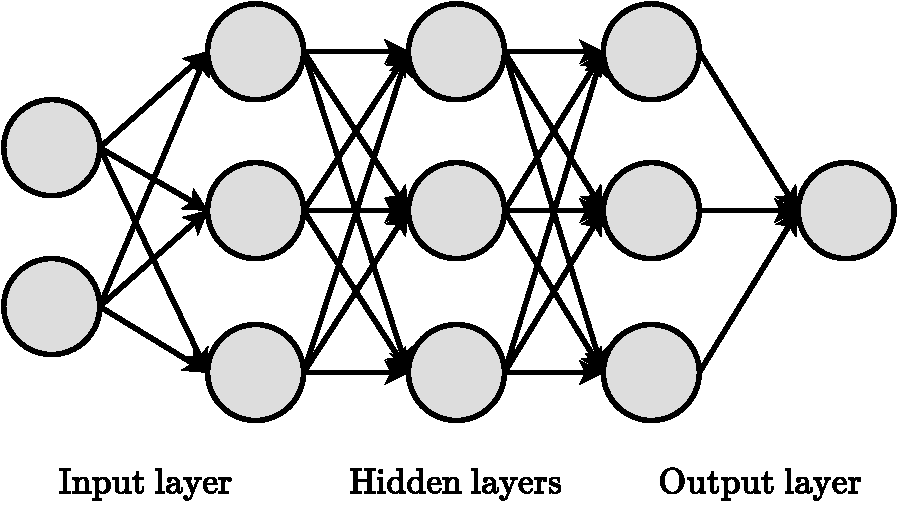
\includegraphics[width=0.5\textwidth]{figures/background/mlp_example}
\caption[Example of a Multi-Layer Perceptron (MLP).]{Example of a Multi-Layer Perceptron (MLP), with two inputs, three hidden layers each made up of three neurons and one output.}
\label{fig:mlp_example}
\end{figure}

However, research by~\cite{telgarsky_representation_2015, telgarsky_benefits_2016} and other works have shown that by increasing the number of neurons per layer, we only obtain a linear increase in the representation power of neural networks. However, by adding more layers, the benefits are \emph{exponential}. In the past decade, this has led to a massive explosion of research in the development of \emph{deep} neural network models with multi-layer architectures. The field had been coined \emph{deep learning} accordingly. Results that models with specific combinations of layers with many different structures perform better than the general MLP are frequent insights obtained from this field of research. In the following paragraphs, we will briefly describe the most common types of layers present in models related to and utilized in this work.

\paragraph{Embeddings} \emph{Embedding layers} are used purely to store embedding vectors and function as a simple lookup table. Their input values denote indices of the columns of a matrix in which the embeddings are stored. In order to obtain the embeddings through matrix multiplication, the indices are \emph{one-hot encoded}: 
\begin{align}
    \begin{split}
        \pmb{\theta}_{\ell} = W \in \mathbb{R}^{D \times N}&, f_{\ell}: \offf{1,\dots,N} \to \mathbb{R}^D, \\
        \forall x \in \offf{1,\dots,N}&, f_{\ell}\of{x, \pmb{\theta}_{\ell}} = W \tilde{\pmb{x}}
    \end{split}
\end{align}
where $\tilde{\pmb{x}} \in \mathbb{R}^N, \tilde{x}_i = \mathbb{I}\of{i = x}$ is the one-hot encoded input, $D$ is the \emph{embedding dimension} and $N$ is the \emph{input dimension} (number of embeddings to store).

\paragraph{Convolution} Unlike for fully-connected layers, where the whole input is linearly combined with the weights, convolutional layers apply a smaller set of weights, called the \emph{filter} or \emph{kernel}, to each smaller section of the input of equal size, using the \emph{discrete convolution operation} in order to obtain the list of outputs. In this manner, the model is more robust to \emph{translations} of the input. The form of this type of layer for one-dimensional input would be: 
\begin{align}
\begin{split}
\pmb{\theta}_{\ell} &= \of{\pmb{w} \in \mathbb{R}^{S}, b \in \mathbb{R}}, f_{\ell}: \mathbb{R}^{D} \to \mathbb{R}^{D-S+1}, \\
\forall i &\in \offf{1,\dots,D-S+1}, y_i = b + \sum_{j=1}^{S}{x_{i+j-1}w_j} 
\end{split}
\end{align}

\paragraph{BatchNorm} \emph{Batch normalization layers} were proposed by~\cite{ioffe_batch_2015} in order to control the statistics (mean/variance) of the neural network activations during training and avoid issues such as parameter gradients decaying to $0$. BatchNorm layers are models that achieve this by learning how to re-normalize their inputs: 
\begin{equation}
\pmb{\theta}_{\ell} = \of{\gamma, \beta}, f_{\ell}\of{\pmb{x}, \pmb{\theta}_{\ell}} = \gamma \odot \frac{\pmb{x}-\hat{\mu}\of{\pmb{x}}}{\sqrt{\hat{\sigma}^2\of{\pmb{x}} + \varepsilon}} + \beta, \varepsilon << 1.
\end{equation}

\paragraph{Dropout} \emph{Dropout layers} were proposed by~\cite{hinton_improving_2012} as a form of regularization for deep neural networks, i.e., they control parameter values in order to avoid the model over-fitting the data. The effect is achieved by randomly selecting input values to be set to $0$ according to a $\text{Bernoulli}\of{p}$ distribution, where the probability $p$ is a hyperparameter.
 
\subsection{Attention}
Attention mechanisms are a particular type of model that can also be used as a neural network layer. The technique is inspired by cognitive attention: the power to focus on only what is essential. Attention layers can be viewed as a generalization of fully connected and convolutional layers. Instead of manually setting which parts of the input should influence which parts of the target, as these two types of layers do, we allow the model to specify this \emph{dynamically}, by assigning \emph{attention weights} for all input-target pairs. Historically, different pathways to calculate the weights have been proposed, but all attention mechanisms follow the same general idea.

To define the general attention mechanism, we will utilize the query-key-value terminology of~\cite{graves_neural_2014} and~\cite{vaswani_attention_2017}, as well as current standards on how to compute the components required for the attention weights. The definition will be given below, while Figure~\ref{fig:attention} provides a visual representation as a summary.

\begin{definition}
An \emph{attention mechanism} is a model $M=\of{\pmb{\theta}, f}$ with the following properties:
\begin{itemize}
\item $\mathcal{X}=\mathbb{R}^{N \times M} \times \mathbb{R}^{N' \times M'}$; 
\item $\pmb{\theta}=\offf{W_Q \in \mathbb{R}^{D \times M}, W_K \in \mathbb{R}^{D \times M'}, W_V \in \mathbb{R}^{D' \times M'}}$, $D, D' \in \mathbb{N}$;
\item The \emph{query matrix} $Q \in \mathbb{R}^{N \times D}$ is computed from the input: $Q = X W_Q^T$;
\item The \emph{key matrix} $K \in \mathbb{R}^{N' \times D}$ and \emph{value matrix} $V \in \mathbb{R}^{N' \times D'}$ are computed from the target: $K=Y W_K^T, V=Y W_V^T$;
\item $f\of{\of{X, Y}, \pmb{\theta}} = A V$, where $A \in \mathbb{R}^{N \times N'}$ is called the \emph{attention matrix} and contains the attention weights;
\item The attention matrix is computed using the queries and keys: 
\begin{align}
\begin{split}
\forall i &\in \offf{1,\dots,N}, j \in \offf{1,\dots,N'}, \\
A_{ij}&=\text{Softmax}_j\of{a\of{Q_i,K_j}}=\frac{e^{a\of{Q_i,K_j}}}{\sum_{r=1}^{N'}{e^{a\of{Q_i,K_r}}}},
\end{split}
\end{align}
where $a: \mathbb{R}^D \times \mathbb{R}^D \to \mathbb{R}$ is some expression that can also be parametrized;
\item Attention mechanisms differ in the choice of $a$, but the simplest commonly used form is \emph{dot-product attention} (\cite{luong_effective_2015}): $a\of{q, k}=q^T k$.
\end{itemize}
\end{definition}

\begin{figure}[H]
\centering
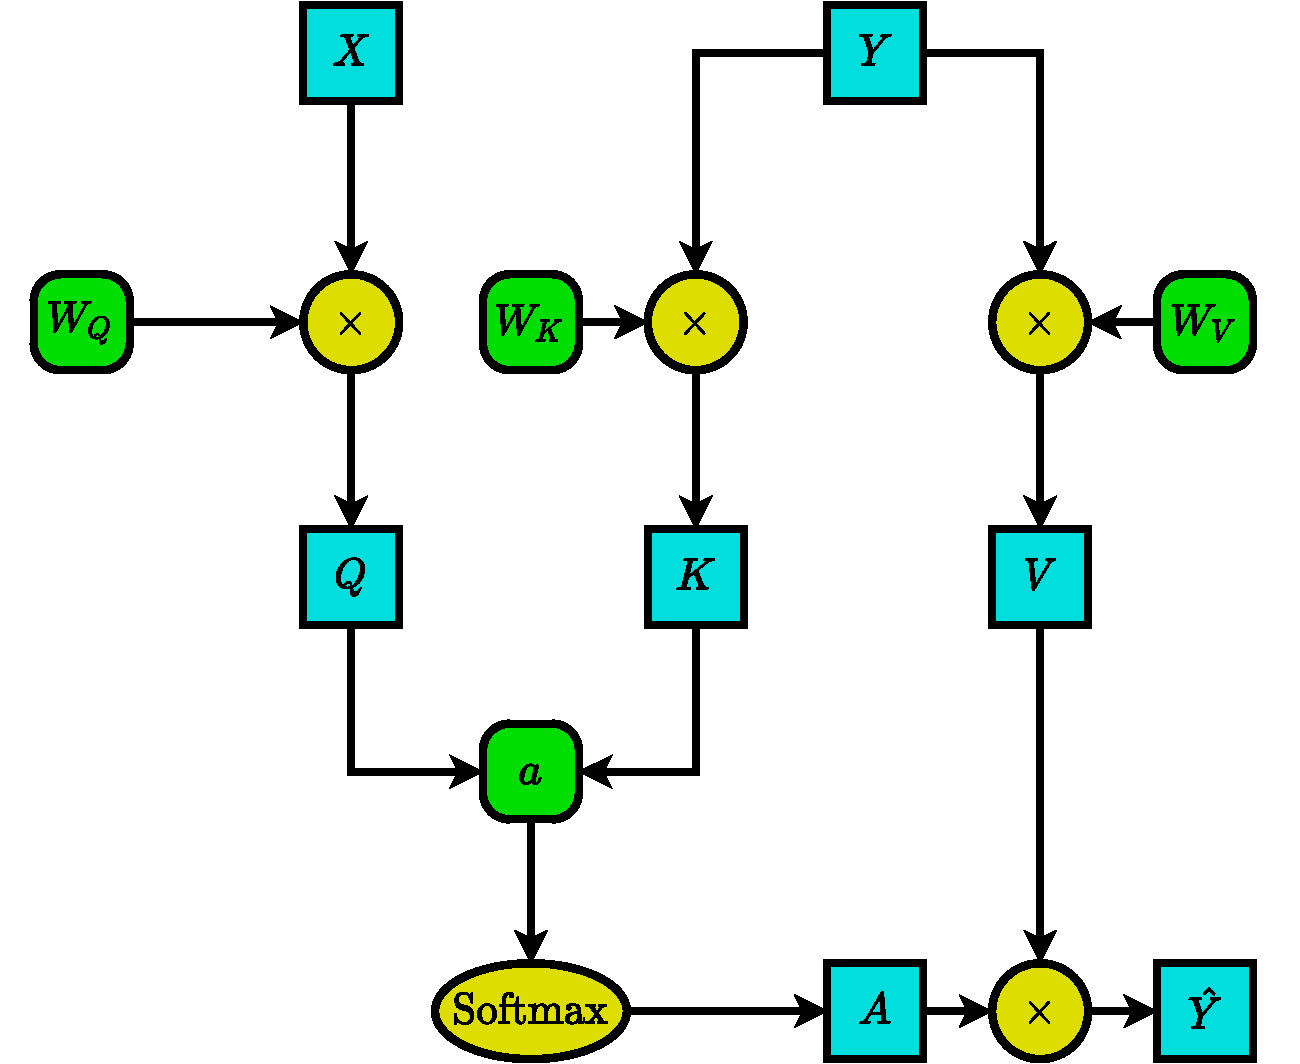
\includegraphics[width=0.75\textwidth]{figures/background/attention.pdf}
\caption[Visualization of a general attention mechanism.]{Visualization of a general attention mechanism.}
\label{fig:attention}
\end{figure}

\subsection{Graph Neural Networks}
Historically, neural network models have seen tremendous success when applied to a highly diverse selection of challenges arising in various scientific disciplines, and graphs are no exception. For more than a decade up until today, research in developing robust neural networks for graph-related tasks has been progressing in parallel with purely graph-embedding-based approaches. However, it is incorrect that these two ideas are disconnected; neural networks for graphs can be generalized beyond the simple single-embedding-layer architecture. Despite the high variety in introduced model design, leading to many model sub-classes, all are usually referred to together with Graph Neural Networks (GNNs).

\cite{battaglia_relational_2018} successfully attempts to aggregate a decade of previous research in graph representation learning using network models into the most general framework that can be used to describe and comprehend the plethora of model designs from a higher-level perspective. The authors explain that the general GNN architecture can be viewed as a composition of a finite number of generalized graph processing models, coined GN blocks. Each GN block receives a graph representation as input and outputs a \emph{refined} representation of the graph, such that the representations evolve from the original discrete entity and relation sets into several layers of improvements to some initial embeddings. 

In order to generalize the structure of GN blocks and the operations that need to be performed, the authors allow the generality of the graph definition as well. Graph nodes and edges are allowed to have a whole collection of \emph{attributes}, not only single type labels, possibly global attributes attached to the whole graph present as well. For a graph $G=\of{V, E}$, let $\pmb{v}_i$ denote the attributes of node $v_i \in V$, $\pmb{e}_{ij}$ the attributes of edge $\of{v_i,v_j}\in E$ and $\pmb{u}$ the global graph attributes. The sequence of operations a general GN block thus has to perform in order to obtain a representation of such rich graphs is visually represented in Figure~\ref{fig:general_gn_block} and formally defined below:
\begin{enumerate}
\item Update edge attributes by applying a mapping model per edge: 

$\forall \of{v_i, v_j} \in E, \pmb{e}'_{ij} = \phi^e\of{\pmb{e}_{ij},\pmb{v}_i,\pmb{v}_j,\pmb{u}}$;
\item Aggregate edge-attributes per node: 

$\forall v_i \in V,\bar{\pmb{e}}'_i = \rho^{e \to v}\of{E'_i}$, where $E'_i = \offf{\of{\pmb{e}'_{ij}, v_i, v_j} \mid v_j \in V}$;
\item Update node attributes by applying a mapping model per node: 

$\forall v_i \in V, \pmb{v}'_i = \phi^v\of{\bar{\pmb{e}}'_i, \pmb{v}_i, \pmb{u}}$;
\item Aggregate edge attributes globally: $\bar{\pmb{e}}'=\rho^{e \to u}\of{E'}$, where $E' = \bigcup_{v_i \in V}{E'_i}$;
\item Aggregate node attributes globally: $\bar{\pmb{v}}'=\rho^{v \to u}\of{V'}$, where $V' = \offf{\pmb{v}'_i \mid v_i \in V}$;
\item Update global attributes by applying a mapping model: $\pmb{u}'=\phi^u\of{\bar{\pmb{e}}', \bar{\pmb{v}}', \pmb{u}}$;
\item Output the new graph representation: $G'=\of{V', E', \pmb{u}'}$.
\end{enumerate}

\begin{figure}%[H]
\centering
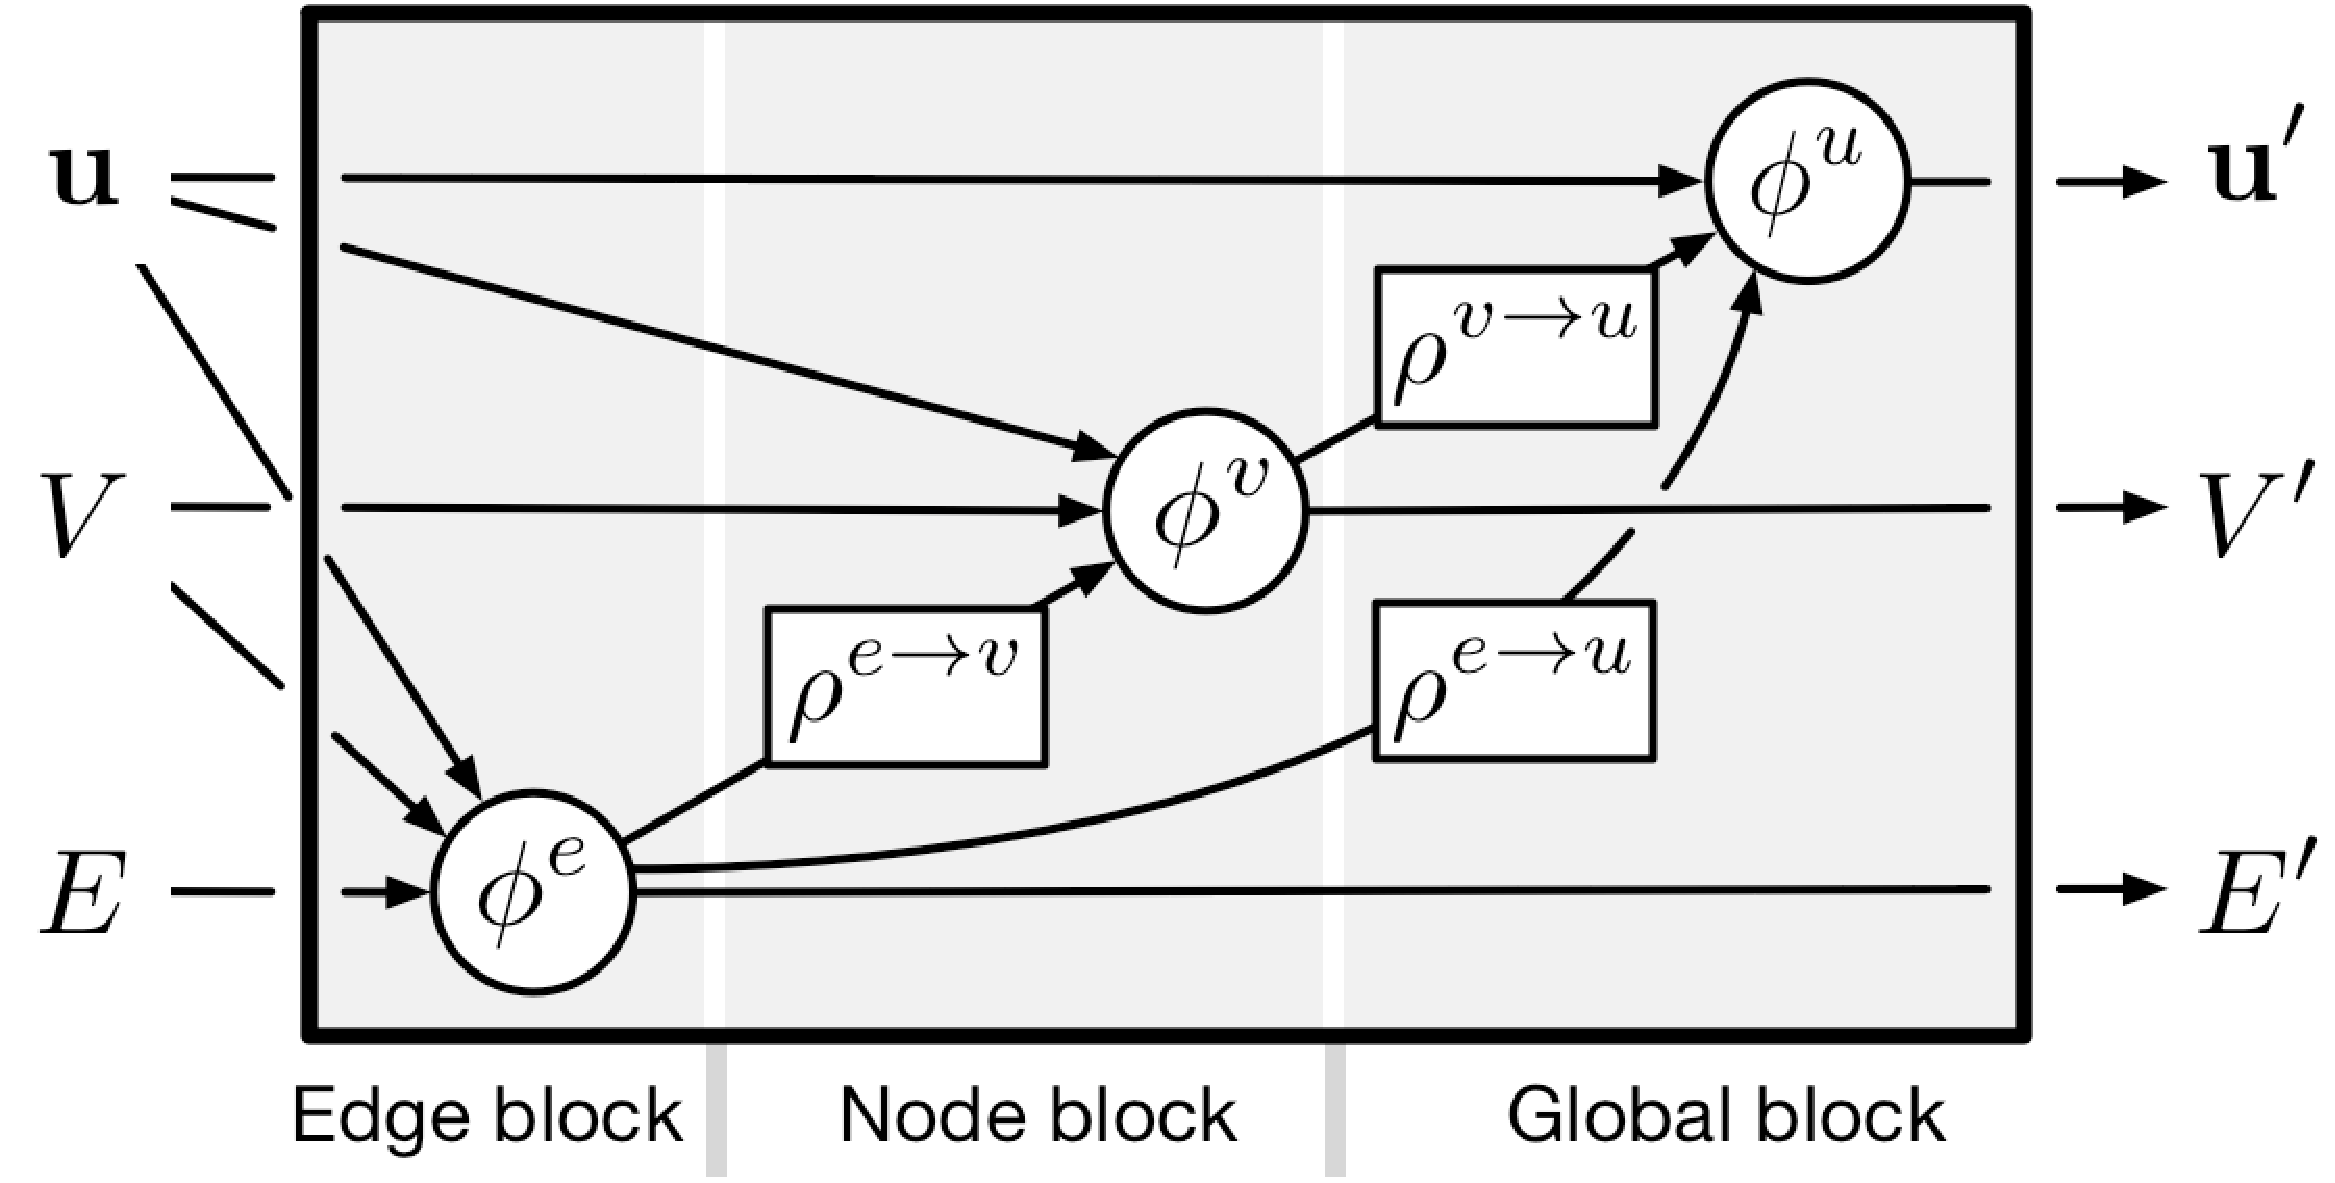
\includegraphics[width=\textwidth]{figures/background/general_gn_block}
\caption[Visualization of the general GN block pipeline.]{Visualization of the general GN block pipeline. Courtesy of~\cite{battaglia_relational_2018}.}
\label{fig:general_gn_block}
\end{figure}

The mapping models $\phi^e, \phi^v, \phi^u$ can potentially be neural networks of any architecture, while for the aggregation functions $\rho^{e \to v},\rho^{e \to u},\rho^{v \to u}$, usually a mean, sum, or max is used.

The proposed framework is helpful in structuring and organizing graph network ideas that can be applied to the most attribute-rich graph.
\chapter{Scalable Knowledge Graph Reasoning}
\label{chp: kg_reasoning}

% \addcontentsline{toc}{chapter}{Scalable Knowledge Graph Reasoning}

This chapter will cover our COINs technique for scalable knowledge graph reasoning, having both theoretical and experimental guarantees, as well as a successful industry application for the Monty knowledge base of Swisscom AG Switzerland. The work which will be discussed here is an improvement, extension and generalization of my master thesis \cite{janchevski_graph_2021}.

\section{Community Informed Graph Embeddings}
\label{sec: coins}

In this section, we present a new method, called COINs for \textbf{CO}mmunity \textbf{IN}formed graph embedding\textbf{s}, to enhance the efficiency of knowledge graph models for link prediction and conjunctive query answering. COINs uses a community-detection-based graph data augmentation and a two-step prediction pipeline: we first achieve node localization through community prediction, and subsequently, we further localize within the predicted community. We establish theoretical criteria to evaluate our method in our specific context and establish a direct expression of the reduction in time complexity. We empirically demonstrate an important scalability-performance trade-off where for the median evaluation sample we preserve 97.18\% of the baseline accuracy in single-hop query answering, for only 7.52\% of the original computational cost on a single-CPU-GPU machine. 

The work described in this section has been accepted for publication as~\cite{janchevski_coins_2025}.

\subsection{Motivation}
Knowledge graphs are a type of database where the general structure is a \emph{network} of \emph{entities}, their semantic \emph{types}, \emph{properties}, and \emph{relationships}; relations are \emph{flexible} through the use of \emph{abstract classes} to represent real-world data from potentially multiple topical domains~\cite{ehrlinger_towards_2016,hogan_knowledge_2020}. Organizations often use knowledge graphs to catalog and analyze relational data. However, scalability becomes a challenge as the graphs can become very large and require significant computational resources.

Almost all existing scaling approaches involve \emph{splitting the enormous graph into disjoint subsets}, followed by distributed training.
For instance, PyTorch-BigGraph~\cite{lerer_pytorch-biggraph_2019} and DGL-KE~\cite{zheng_dgl-ke_2020} are distributed-algorithm-system frameworks that can scale the implementation of graph neural networks with distributed execution over billion-scale graphs.
On the other hand, SMORE~\cite{ren_smore_2021} focuses on model parallelization and employs an efficient algorithm for sampling data. CARL-G~\cite{shiao_carl-g_2023} provides similar speed-ups in data sampling to SMORE, but applies only to a non-contrastive setting, and both guarantee acceleration only during training. tf-GNN~\cite{ferludin_tf-gnn_2022} mainly focuses on accelerating the sampling of k-hop neighborhoods of nodes during distributed training.

To this end, we present COINs ({\bf CO}mmunity {\bf IN}formed graph embedding{\bf s}) in a distinct, low-resource setting for transductive knowledge graph reasoning model optimization, inference, and evaluation in the contrastive learning setting. We contend that this setting remains elusive to the scalable approaches above, which require a minimum (but still a formidable) level of computational power, and offers new insights to accelerate graph inference. 

In stark contrast, we consider a setting, for instance, where even model evaluation is a major hurdle. Indeed, for the evaluation procedure, the state-of-the-art approaches above either apply data parallelization over a large cluster of machines (as for GATNE~\cite{cen_representation_2019}) or use a random subset of the graph (as noted in~\cite{ren_smore_2021}). On the other hand, NodePiece~\cite{galkin_nodepiece_2022} and EARL~\cite{chen_entity-agnostic_2023} are works that, like ours, do not disregard resource efficiency and reduce the overall computational complexity by admitting a degree of sacrifice in performance. We will argue that, nevertheless, when compared to COINs, they fail to retrieve as much of the baseline performance, only focus on reducing the model size, and do not consider acceleration in inference.

Before explicitly stating our contributions below, we will first establish the background and introduce the preliminaries in the sequel. 

% \vspace{-3mm}
\subsection{Background}
\label{sec:background}
\subsubsection{Problem and Challenges}

Performing knowledge graph inference requires solving link prediction and query answering. Given a dataset of entity-relation-entity triplets, labeled positive or negative according to whether they have originated from the knowledge graph or not, link prediction involves predicting these labels. 

On the other hand, given a list of logical queries extracted from the knowledge graph, the query answering task requires ranking for \emph{each} query \emph{all} of the entities in the graph according to how likely they are to be its correct answer. Thus, compared to link prediction, this task is much more computationally complex, as the largest contributor to the number of model inference calls is the size of the graph. Our work aims to reduce this factor significantly.

\subsubsection{Preliminaries}

Mathematically, we can represent knowledge graphs with AMHENs:
\begin{definition}
An \emph{Attributed Multiplex HEterogeneous Network (AMHEN)} is a graph where each entity (node) in a set $V$ has attributes and each relation (edge) in a set $E$ has a type label~\cite{liu_ahng_2019,cen_representation_2019}. 

Formally, first, a finite set of \emph{relation types} is defined $R = \offf{r_1,r_2,\dots}$, and the edge labeling is represented through the mathematical relation $E_R \subseteq V \times R \times V$, called the \emph{set of relation triplets}:  $E_R = \offf{\of{h,r,t} \mid h,t \in V, \of{h,t} \in E, r \in R}$. Entity/node attributes can be collected, e.g., in a matrix $\mathbf{X} \in \mathbb{R}^{\abs{V} \times F}$, with $F$ as the feature dimension. 

Usually, the nodes $h$ and $t$ in the triplets are referred to as the \emph{head} and \emph{tail} of the relations, respectively. The attributed multiplex heterogeneous network is the new collection $\of{V, E_R, R, \mathbf{X}}$.
\end{definition}

\begin{definition}
    A \emph{query} of the knowledge graph $G=\of{V, E_R, R, \mathbf{X}}$ is the collection $q=\of{\mathcal{A}_q, G_q}$ of a set $\mathcal{A}_q \subseteq V$ of \emph{anchor} (input) entities and $G_q: \mathcal{A}_q \to \mathcal{P}\of{V}$, a mapping visualized via a \emph{computational graph} in the form of a DAG informing how to obtain \emph{answer} entities to the query starting from the anchors, where during this process all of the nodes in $q$ get labeled with sets of entities from $V$. 
    
    In the special case of \emph{conjunctive logical queries}, the edges in $q$ represent either \emph{relation projection} operations $P: \mathcal{P}\of{V} \times R \to \mathcal{P}\of{V}$ (map head to tail along a relation) or \emph{intersection} operations $I: \mathcal{P}\of{\mathcal{P}\of{V}} \to \mathcal{P}\of{V}$ (classical $\cap$), specializing the query mapping as $G_q\of{\mathcal{A}_q;P,I}$~\cite{ren_query2box_2020}.
    \label{def:query}
\end{definition}
Figure~\ref{fig:query_structures} visualizes the computational structures of the conjunctive queries we considered. To give an example of the notation from Definition~\ref{def:query}, the general form of an ip-type conjunctive query $q$ has: 
\begin{equation}
    \mathcal{A}_q=\offf{v_1,v_2}, G_q\of{\offf{v_1,v_2}}=P\of{I\of{\offf{P\of{\offf{v_1},r_1},P\of{\offf{v_2},r_2}}},r_3},
\end{equation}
where $v_1,v_2 \in V, r_1,r_2,r_3 \in R$ are any entities and relations from $G$.

\begin{figure}[H]
    \centering
    \includegraphics[width=0.75\textwidth]{figures/coins/query\_structures.pdf}
    \caption[Various possible computational graph structures of conjunctive knowledge graph queries.]{Various possible computational graph structures of conjunctive knowledge graph queries. Blue nodes indicate query anchors/inputs, green ones are their answers, while the rest are intermediate results. Solid edges represent relation projections, dashed edges represent intersection operations.}
    \label{fig:query_structures}
\end{figure}

Graphs are discrete structures, while the majority of machine learning models work exclusively with real-valued continuous inputs. Therefore, we have to construct a mapping from the graph elements to a numeric vector space, such that the output vectors encode the graph structure in the form of algebraic constraints.
\begin{definition}
Given a knowledge graph $G = \of{V, E_R, R, \mathbf{X}}$, in general one defines a \textit{knowledge graph embedding model}~\cite{ji_survey_2022,liang_survey_2024,ren_query2box_2020} as the collection of an entity embedding model $g_V: V \to \mathcal{E}$, relation embedding model $g_R: R \to \mathcal{R}$, relation projection embedding model $g_P: \mathcal{E} \times \mathcal{R} \to \mathcal{E}$, intersection embedding model $g_I: \mathcal{\mathcal{E}}^{\mathbb{N}} \to \mathcal{E}$ and a scoring function $f: \mathcal{E} \times \mathcal{E} \to \mathbb{R}$, all potentially parametrized. Outputs $\mathbf{v} = g_V\of{v}, \mathbf{r} = g_R\of{r}, \mathbf{q}, \mathbf{a}, \dots$ are referred to as \emph{embeddings}. Most often $\mathcal{E}, \mathcal{R} \subseteq \mathbb{R}^D$ or $\mathbb{C}^D$, where $D$ is the \emph{embedding dimension}. 
\end{definition}

Most embedding models are optimized using a contrastive likelihood based on $f$:
\begin{definition}
\label{def:contrastive_loss}
    Given the model's scoring function $f$ and the embedding representation of a single \emph{positive} query-answer pair $\of{q, a}$ and a set of $m$ \emph{negative examples} $\offf{a'_i}_{i=1}^{m} \subseteq V \setminus \offf{a}$ (wrong answers to the query), the \emph{contrastive learning loss} terms and final value take the common form ($\sigma$ denoting the sigmoid function):
    \begin{align}
    \begin{split}
    \label{eq:contrastive_loss}
        \tilde{\mathcal{L}}\of{\mathbf{q}, \mathbf{a}, y}&=-\log{\sigma{\of{y \cdot f\of{\mathbf{q},\mathbf{a}}}}}\\
        \mathcal{L}\of{\mathbf{q}, \mathbf{a}, \offf{\mathbf{a}'_i}_{i=1}^{m}}&=\tilde{\mathcal{L}}\of{\mathbf{q}, \mathbf{a}, 1} + \frac{1}{m}\sum_{i=1}^{m}{\tilde{\mathcal{L}}\of{\mathbf{q}, \mathbf{a}'_i, -1}}
        \end{split}
    \end{align}
\end{definition}

\begin{definition}
    Given a dataset $\mathcal{D}=\offf{\of{h_i, r_i, t_i}}_{i=1}^{N}$ of head-relation-tail triplets and labels $\offf{y_i}_{i=1}^{N}$ indicating whether each triplet was extracted from the knowledge graph or randomly formed, a \emph{link predictor} $\ell: V \times R \times V \to \mathbb{R}$ is a model that aims to predict the label $y_i$ of each triplet $\of{h_i,r_i,t_i}$ by estimating the likelihood of it originating from the knowledge graph.
\end{definition}

\begin{definition}
    Given a dataset $\mathcal{D}=\offf{\of{q_i, a_i}}_{i=1}^{N}$ of query-answer pairs extracted from the knowledge graph, \emph{query answering} entails predicting the answer entity $a_i$ given the query information $q_i$ as input. Classically, this is operationalized by forming the set $\hat{\mathcal{D}}_i=\offf{\of{q_i, v}}_{v \in V}$ by combining the query with every possible answer, then the predicted answer is the one that maximizes a scoring model: $\hat{a}_i = \argmax_{v \in V}{S\of{q_i,v}}$.
\end{definition}

\subsubsection{Contributions}
Most previous work on knowledge graph inference acceleration~\cite{lerer_pytorch-biggraph_2019,zheng_dgl-ke_2020,ren_smore_2021} focuses on \emph{model-free} solutions relying on hardware and software for distribution and parallelization. Few \emph{model-based} approaches exist that do take resource limitations into account, balancing the model's computational cost with performance, with benefits scaling up with graph size instead of number of compute units.

NodePiece~\cite{galkin_nodepiece_2022} and EARL~\cite{chen_entity-agnostic_2023} propose accelerating knowledge graph prediction tasks by reducing the total number of embedding parameters required. This is done by selecting only certain \enquote{reserved} entities to be a part of a vocabulary $\mathcal{T} \subseteq V$, then only pre-computing the vocabulary embeddings. Embeddings for non-vocabulary entities must be obtained on the spot by selecting for each of them $\tau$ reserved nodes from the vocabulary (via a specific assignment rule) and then re-encoding the sequence of the $\tau$ embeddings. Both works thus require at least $\abs{\mathcal{T}} + \tau\of{\abs{V}-\abs{\mathcal{T}}}N$ embedding computations during evaluation, many times larger than the baseline cost of $\abs{V}N$.

On the other hand, our contributions can be summarized as follows:
\begin{enumerate}[I.]
    \item COINs are a \emph{model-based} approach that introduces a novel integration of \emph{community structure information} into optimization and inference to achieve significant acceleration even with limited resources, and balancing speed-up in the best way with baseline performance retrieval and model size;
    \item We derive upper and lower bounds for the total number of embeddings that must be computed during evaluations. By being community-adaptive, our algorithm operates near the lower bound, thereby achieving the best possible speed-ups in practice during evaluation. 
\end{enumerate}
\subsubsection{Scalable query answering evaluation}
Assume that we possess a mapping $c: V \to \mathcal{C}$, assigning knowledge graph entities into one of $\abs{\mathcal{C}} = K \leq \abs{V}$  groups, similar to some previous work~\cite{lerer_pytorch-biggraph_2019,zheng_dgl-ke_2020}. 
With $c$, we construct an alternative two-step query answering procedure:
 \begin{enumerate}
     \item Map the input $\of{q, a}$ to a group-level query-answer pair $\of{q^{\of{C}}, c\of{a}}$, and predict $c\of{a}$ by scoring all $K$ possible answer groups;
     \item Search for the correct answer $a$ only among the entities $\hat{a}$ with $c\of{\hat{a}}=c\of{a}$.
 \end{enumerate}

\subsubsection{Optimal partition structure}

First note that the mapping $c$ induces a \emph{disjoint partition} of the entity set $V$. Namely, if we construct the sets $C_k = \offf{v \in V \mid c\of{v}=k}, k \in \mathcal{C}$, then $\bigcup_{k=1}^{K}{C_k}=V$ and $\forall i,j \in \mathcal{C},i \neq j, C_i \cap C_j = \emptyset$. 

By analyzing in detail the computational complexity of our new evaluation method, one can easily assess the quality of any such disjoint partition. 
Proposition~\ref{proposition:complexity} provides our main result. The proof is available in Appendix~\ref{sec:appendix_proofs}.
\begin{proposition}
\label{proposition:complexity}
Let $\abs{C_k}$ denote the size of node group $k$ and $N_k=\abs{\offf{\of{q, a} \in \mathcal{D} \mid c\of{a}=k}}$ denote the number of evaluation samples with query answers in node group $k$. The number of query embedding vectors computed in total during evaluation has the following form and bounds:
\begin{equation}
\label{eq:complexity_and_bounds}
2 N \sqrt{\abs{V}} \leq \sum_{k=1}^{K}{\of{K+\abs{C_k}}N_k} \leq N \of{\abs{V} + 1} 
\end{equation}
\end{proposition}

\subsubsection{Query locality}
The lower bound of equation \eqref{eq:complexity_and_bounds} above states that it is possible to achieve a $\sqrt{\abs{V}}$ dependence in evaluations, while the scalable approaches we have discussed so far have a linear dependence on ${\abs{V}}$. 
However, to minimally affect the baseline performance, we must consider the partitioning quality from the perspective of preserving the relational structure. 

What previous works often fail to consider is that an arbitrary assignment might be \emph{arbitrarily non-local}. Formally, if we construct the set 
\begin{equation}
V^*\of{c}=\offf{v \in V \mid \exists \of{u,r}, E_R \cap \offf{\of{v,r,u}, \of{u, r, v}} \neq \emptyset, c\of{u} \neq c\of{v}}    
\end{equation}
of entities that participate in between-group relations, then we must have both minimal $\abs{V^*\of{c}}$ as well as minimal total evaluation cost (Proposition~\ref{proposition:complexity}). 

In this case, the search for the true answer to a query will be most often localized to a small neighborhood in the knowledge graph, a significantly easier problem. Equivalently, one prefers a mapping $c$ such that more relations are present \emph{within} the entity sets $C_k$ than \emph{between} them. 

Unfortunately, achieving good localization is an NP-hard problem, but research in the fields of \emph{community detection} and \emph{minimal cuts} for graphs has yielded efficient heuristic algorithms. 

Such is the Leiden algorithm for community detection~\cite{traag_louvain_2019}, the current state-of-the-art, based on heuristic maximization of the Constant Potts Model~\cite{traag_narrow_2011} version of the modularity score~\cite{blondel_fast_2008}, with further manual refinement to guarantee well-connected communities. The single \enquote{resolution} hyperparameter of the algorithm is the only degree of freedom controlling the community assignment quality. To this end, our work represents a novel application of Leiden communities to knowledge graph inference. 

On the other hand, the METIS algorithm for graph partitioning~\cite{karypis_fast_1998}, employed also in~\cite{zheng_dgl-ke_2020}, strives towards minimal graph cuts. For some experiments, we considered it as an alternative to Leiden to estimate the effect of the choice of graph-splitting method.

\subsection{Methodology}
\label{sec:methodology}

\subsubsection{Community detection}

Given a knowledge graph $\of{V, E_R, R, \mathbf{X}}$, the first step we employ is to execute the Leiden community detection algorithm to obtain a good node-to-community mapping $c: V \to \mathcal{C}$. 

For our COINs technique, based on the obtained community assignment map $c$ we extract further discrete information of great utility for efficient training and evaluation. $c$ coarsens $\of{V, E_R}$ into a \emph{community-level interaction graph}: 
\begin{equation}
V^{\of{C}} = \mathcal{C}, E^{\of{C}}_R = \offf{\of{c\of{u},r,c\of{v}} \mid \of{u,r,v} \in E_R}.    
\end{equation}
In addition, one can compute the \emph{inter-community mapping} $z^*: V \to V_{\omega}^*$:
\begin{equation}
    z^*\of{v}=\begin{cases} v, & \text{ if } v \in V^* \\ \omega, & \text{ otherwise} \end{cases},
\end{equation}
where $V_{\omega}^* = V^* \cup \offf{\omega}$ and $\omega$ is a padding node representing all nodes in $V \setminus V^*$.

\subsubsection{COINs training \& evaluation}

\begin{figure}%[H]
    \centering
    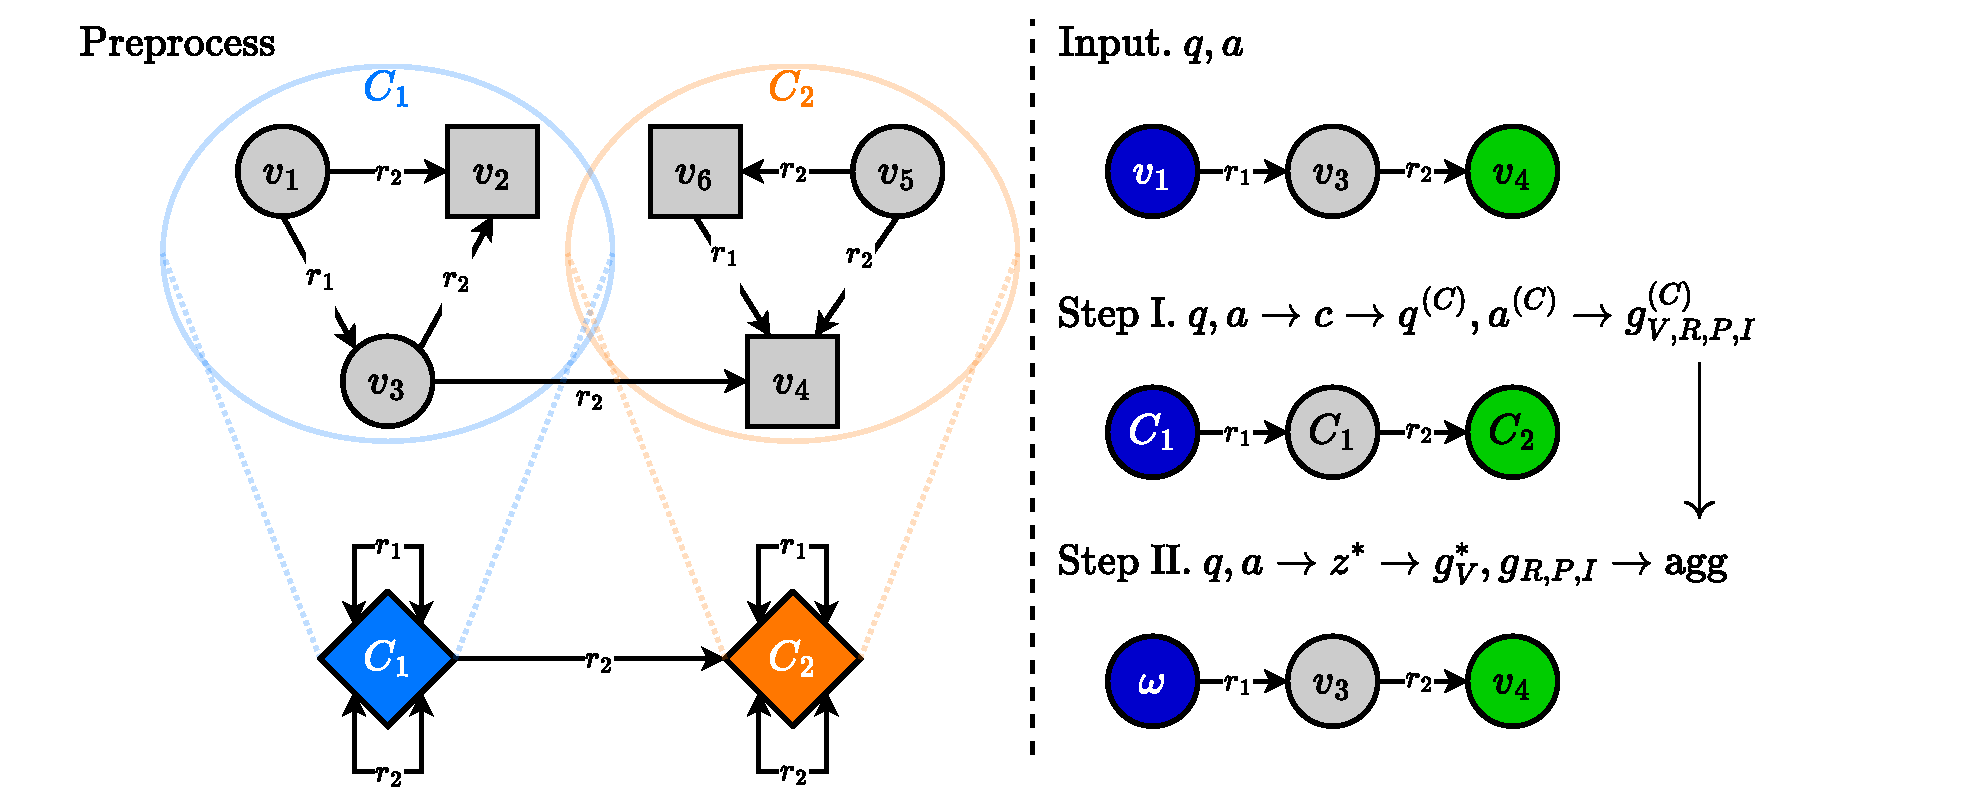
\includegraphics[width=0.75\textwidth]{figures/coins/coins.pdf}
    \caption[Example of a preprocessed knowledge graph and the COINs representation process on an example query.]{Left: example of a preprocessed knowledge graph, showing its transformation into a community-level graph, with $\abs{V}=6, \abs{E_R}=7, T=2, \abs{R}=2, K=2, \abs{V^*}=2$. Right: the COINs representation process on an example inter-community 2p-query of the graph.}
    \label{fig:community_preprocessing}
\end{figure}

Let $\mathcal{F}$ denote the class of knowledge graph embedding models whose scalability we wish to improve, and $\tilde{\mathcal{L}}: \mathcal{E} \times \mathcal{E} \times \offf{-1,1} \to \mathbb{R}$ be the per-sample contrastive loss term minimized during training such models (eq. \eqref{eq:contrastive_loss}). 

COINs requires the optimization of the following models sampled from $\mathcal{F}$:
\begin{itemize}
    \item {Community-level embedders}: $g_V^{\of{C}}: \mathcal{C} \to \mathcal{E}, g_R^{\of{C}}: R \to \mathcal{R}, g_P^{\of{C}}: \mathcal{E} \times \mathcal{R} \to \mathcal{E}, g_I^{\of{C}}: \mathcal{E}^{\mathbb{N}} \to \mathcal{E}$;
    \item {Intra-community entity embedders}: $g_V^{\of{k}}: C_k \to \mathcal{E}, \forall k \in \mathcal{C}$;
    \item {Inter-community entity embedder}: $g_V^{*}: V_{\omega}^* \to \mathcal{E}$. 
    \item {Node-level relation and query embedders}: $g_R: R \to \mathcal{R}, g_P: \mathcal{E} \times \mathcal{R} \to \mathcal{E}, g_I: \mathcal{E}^{\mathbb{N}} \to \mathcal{E}$
\end{itemize}

Additional parameters are: a {node feature embedding matrix} $\mathbf{W} \in \mathbb{R}^{D \times F}$ and {node/relation embedding aggregation weights} $\mathbf{w} \in \mathbb{R}^{3}, \mathbf{w}_R \in \mathbb{R}^{2}$.

Algorithm~\ref{algorithm:baseline} presents the baseline inference steps required, Algorithm~\ref{algorithm:coins} details the knowledge graph query representation steps for COINs, utilizing the constructed sub-models, while Figure~\ref{fig:community_preprocessing} provides a visualization of our community-based preprocessing and query representation on a small example. 

\begin{algorithm}%[H]
    \caption{Base knowledge graph representation}
    \label{algorithm:baseline}
    \begin{algorithmic}[1]
    \STATE{\textbf{input} $\of{q, a}$, $y \in \offf{-1,1}$}
    \STATE{$\mathbf{R}\gets\off{g_R\of{r}}_{r \in R}$}
    \STATE{$\mathbf{a} \gets g_V\of{a}, \mathbf{A}\gets\off{g_V\of{v}}_{v \in \mathcal{A}_{q}}$}
    \STATE{$\mathbf{q} \gets G_{q}\of{\mathbf{A};\of{\mathbf{R},g_P},g_I}$}
    \STATE{\textbf{return} $\tilde{\mathcal{L}}\of{\mathbf{q}, \mathbf{a}, y}$}
    \end{algorithmic}
\end{algorithm}
 
\begin{algorithm}%[H]
\caption{COINs knowledge graph representation}
\label{algorithm:coins}
\begin{algorithmic}[1]
\STATE{\textbf{input} $\of{q, a}$, $y \in \offf{-1,1}$, $c:V \to \mathcal{C}$, $z^*: V \to V_{\omega}^*$, $\alpha \in \of{0,1}$}
\STATE{$\mathbf{R}^{\of{C}} \gets \off{g^{\of{C}}_R\of{r}}_{r \in R}, \tilde{\mathbf{R}} \gets \off{g_R\of{r}}_{r \in R}$}
\STATE{$\mathbf{R} \gets \ang{ \mathrm{Softmax}\of{\mathbf{w}_R}, \off{\mathbf{R}^{\of{C}}, \tilde{\mathbf{R}}} }$}
\STATE{$q^{\of{C}} \gets \of{\off{c\of{v}}_{v \in \mathcal{A}_q},G_q}$}
\STATE{$\mathbf{a}^{\of{C}} \gets g^{\of{C}}_V\of{c\of{a}}, \mathbf{A}^{\of{C}} \gets \off{g^{\of{C}}_V\of{k}}_{k \in \mathcal{A}^{\of{C}}_{q}}$}
\STATE{$\mathbf{q}^{\of{C}} \gets G_{q}\of{\mathbf{A}^{\of{C}};\of{\mathbf{R}^{\of{C}},g_P^{\of{C}}},g_I^{\of{C}}}$}
\IF{$\forall v \in q, c\of{v}=c\of{a}$}
\STATE{$\tilde{\mathbf{a}} \gets g^{\of{c\of{a}}}_V\of{a}, \tilde{\mathbf{A}} \gets \off{g^{\of{c\of{a}}}_V\of{v}}_{v \in \mathcal{A}_{q}}$}
\ELSE
\STATE{$\tilde{\mathbf{a}} \gets g^{*}_V\of{z^*\of{a}}, \tilde{\mathbf{A}}\gets\off{g^{*}_V\of{z^*\of{v}}}_{v \in \mathcal{A}_{q}}$}
\ENDIF
\STATE{$\mathbf{a} \gets \ang{\mathrm{Softmax}\of{\mathbf{w}}, \off{\mathbf{W} \mathbf{x}_{a}, \mathbf{a}^{\of{C}}, \tilde{\mathbf{a}}}}, \mathbf{A} \gets \ang{ \mathrm{Softmax}\of{\mathbf{w}}, \off{\mathbf{W} \mathbf{x}_{v}}_{v \in \mathcal{A}_{q}}, \mathbf{A}^{\of{C}}, \tilde{\mathbf{A}} }$}
\STATE{$\mathbf{q}\gets G_{q}\of{\mathbf{A};\of{\mathbf{R},g_P},g_I}$}
\STATE{\textbf{return} $\tilde{\mathcal{L}}_{\text{COINs}}\of{\mathbf{q}, \mathbf{a}, y}=\of{1-\alpha} \tilde{\mathcal{L}}\of{\mathbf{q}^{\of{C}}, \mathbf{a}^{\of{C}}, y} + \alpha \tilde{\mathcal{L}}\of{\mathbf{q}, \mathbf{a}, y} $}
\end{algorithmic}
\end{algorithm} 
This new construction has several desirable properties, unlike the baseline: 
\begin{enumerate}
    \item Queries spanning multiple communities are treated differently, allowing for greater generalization; 
    \item $K + \max{\of{\max_{k=1}^{K}{\abs{C_k}},\abs{V^{*}} + 1}}$ will be the maximum number of entity embeddings to compute for each training iteration instead of the baseline $\abs{V}$, an overall lower time and memory cost;
    \item The community representation learning will be performed jointly with the node-level, due to the softmax-weighted embedding refinement linking them both, allowing for greater adaptivity;
\end{enumerate}

Observe that the total number of COINs node embeddings for a graph is 
\begin{equation}
    \abs{\boldsymbol{\theta}} = K + \sum_{k=1}^{K}{\abs{C_k}} + \abs{V^*} + 1 = K + \abs{V} + \abs{V^*} + 1,
\end{equation}
compared to just $\abs{V}$ node embeddings in the baseline. Thus, using a partitioning that keeps $\abs{V^*} \ll \abs{V}$ has benefits in limiting model size as well. 

Let now $S_C$ denote a learned scoring model for community-level query-answer pairs, obtained after extending the community-level COINs sub-models into a classifier, with $S_V$ the analog for the final node-level query answer scoring. Then, one can implement the proposed novel scalable query answering procedure via Algorithm~\ref{algorithm:scalable_query_answering}.

\begin{algorithm}[H]
\caption{COINs query answering evaluation}
\label{algorithm:scalable_query_answering}
\begin{algorithmic}[1]
\STATE{\textbf{input} test set $\mathcal{D}=\offf{\of{q_i, a_i}}_{i=1}^{N}$, scorers $S_C, S_V$}
\FOR{$i \gets 1$ to $N$}
\STATE{$q^{\of{C}}_i \gets \of{\off{c\of{v}}_{v \in \mathcal{A}_{q_i}},G_{q_i}}$}
\STATE{$s_C \gets \off{S_C\of{q^{\of{C}}_i, k}}_{k \in \mathcal{C}}$}
\STATE{$\rho^{\of{i}}_{C} \gets \mathrm{Rank}\of{c\of{a_i},s_C}$}
\STATE{$F_i \gets \sum_{1 \leq j < \rho^{\of{i}}_{C}}{\abs{C_{\mathrm{IndexRank}\of{j,s_C}}}}$}
\STATE{$s_V \gets \off{S_V\of{q_i, v}}_{v \in C_{c\of{a_i}}}$}
\STATE{$\tilde{\rho}^{\of{i}} \gets \mathrm{Rank}\of{a_i,s_V}$}
\STATE{$\rho^{\of{i}} \gets F_i + \tilde{\rho}^{\of{i}}$}
\ENDFOR
\STATE{\textbf{return} $\off{\rho^{\of{i}}}_{i=1}^{N}$}
\end{algorithmic}
\end{algorithm} 

\subsubsection{Tradeoff analysis}

The primary limitation of the COINs evaluation procedure is that incorrect community prediction can result in many nodes being returned as false positives (large $F_i$ term in Algorithm~\ref{algorithm:scalable_query_answering}). This conditional nature of the prediction is the main reason for expecting lower performance compared to the baseline. 

However, as community ranks approach 1, we can much more quickly obtain model predictions with fewer and fewer drawbacks for large graphs. Thus, we prove Proposition~\ref{proposition:condition_applicability}, which quantifies under which conditions the application of COINs is feasible, by theoretically analyzing the tradeoff between the possible scalability benefits and performance losses. 

The general takeaway is that one must \emph{per-community} consider the ratio between acceleration factors and relative error in performance metrics, with specific weight values for aggregating these comparisons to obtain a final conclusion through a simple inequality test.


\subsubsection{Distributed extension}

As previously mentioned, previous work mainly solves the problem of query answering scalability by distributing the knowledge graph embedding model across many compute units. Both data and model parallelism are almost fully achieved in this manner; however, the acceleration is always only at best linear with respect to the number of machines available. As such, to scale to very large knowledge graphs, a very large cluster of at least hundreds of machines is required. In this part of the thesis, I will suggest how to utilize available computational resources more efficiently by extending COINs to the distributed learning setting.

Namely, the COINs submodel structure naturally permits partial model parallelism in addition to the acceleration incurred from the two-step inference process. The intra-community and inter-community models used during step 2 of the process are, by design, independent. This is due to the fact that each of those models trains and predicts over a disjoint subset of the knowledge graph edges. As such, Step 2 can be completely parallelized across multiple machines by assigning to each intra-community or inter-community model a dedicated compute unit. The only unavoidable bottleneck is having to sequentially wait for the community prediction of Step 1 to finish, in order to have the information to which machine a data point needs to be communicated.

The distributed COINs architecture is proposed to be as follows. Let $U$ be a finite set of compute units available to the application, and let $\mathcal{M} \subset \mathcal{F}$ be the full set of COINs submodels. The assignment of COINs models to units will be represented through the mapping $u: \mathcal{M} \to U$. First, select a machine $u^* \in U$ to serve as the \emph{leader} node. The leader performs Step 1, sends and receives data between itself and the other machines to orchestrate Step 2, and performs the final aggregation steps. Formally, we fix these assignments:
\begin{equation}
u\of{g_V^{\of{C}}}=u\of{g_R^{\of{C}}}=u\of{g_P^{\of{C}}}=u\of{g_I^{\of{C}}}=u\of{g_R}=u\of{g_P}=u\of{g_I}=u\of{\mathbf{W}}=u\of{\mathbf{w}}=u\of{\mathbf{w}_R}=u^*.
\end{equation}
Then, with this setup, Algorithm~\ref{algorithm:coins_distributed} details the distributed version of Algorithms~\ref{algorithm:coins}. For easier comparison, I color-highlight the required changes for the distributed extension.

\begin{algorithm}[ht!]
\caption{Distributed COINs knowledge graph representation}
\label{algorithm:coins_distributed}
\begin{algorithmic}[1]
\STATE{\textcolor{blue}{\textbf{on} $u^*$:}}
\STATE{\textbf{input} $\of{q, a}$, $y \in \offf{-1,1}$, $c:V \to \mathcal{C}$, $z^*: V \to V_{\omega}^*$, $\alpha \in \of{0,1}$}
\STATE{$\mathbf{R}^{\of{C}} \gets \off{g^{\of{C}}_R\of{r}}_{r \in R}, \tilde{\mathbf{R}} \gets \off{g_R\of{r}}_{r \in R}$}
\STATE{$\mathbf{R} \gets \ang{ \mathrm{Softmax}\of{\mathbf{w}_R}, \off{\mathbf{R}^{\of{C}}, \tilde{\mathbf{R}}} }$}
\STATE{$q^{\of{C}} \gets \of{\off{c\of{v}}_{v \in \mathcal{A}_q},G_q}$}
\STATE{$\mathbf{a}^{\of{C}} \gets g^{\of{C}}_V\of{c\of{a}}, \mathbf{A}^{\of{C}} \gets \off{g^{\of{C}}_V\of{k}}_{k \in \mathcal{A}^{\of{C}}_{q}}$}
\STATE{$\mathbf{q}^{\of{C}} \gets G_{q}\of{\mathbf{A}^{\of{C}};\of{\mathbf{R}^{\of{C}},g_P^{\of{C}}},g_I^{\of{C}}}$}
\IF{$\forall v \in q, c\of{v}=c\of{a}$}
\STATE{\textcolor{blue}{\textbf{async send} $\of{\mathcal{A}_q, a} \to u\of{g_V^{c\of{a}}}$}}
\STATE{\textcolor{blue}{\textbf{on } $u\of{g_V^{c\of{a}}}$:}}
\STATE{$\tilde{\mathbf{a}}\gets g^{\of{c\of{a}}}_V\of{a}, \tilde{\mathbf{A}} \gets \off{g^{\of{c\of{a}}}_V\of{v}}_{v \in \mathcal{A}_{q}}$}
\STATE{\textcolor{blue}{\textbf{async send} $\of{\tilde{\mathbf{A}}, \tilde{\mathbf{a}}} \to u^*$}}
\ELSE
\STATE{\textcolor{blue}{\textbf{async send} $\of{\mathcal{A}_q, a} \to u\of{g_V^{*}}$}}
\STATE{\textcolor{blue}{\textbf{on } $u\of{g_V^{*}}$:}}
\STATE{$\tilde{\mathbf{a}} \gets g^{*}_V\of{z^*\of{a}}, \tilde{\mathbf{A}} \gets \off{g^{*}_V\of{z^*\of{v}}}_{v \in \mathcal{A}_{q}}$}
\STATE{\textcolor{blue}{\textbf{async send} $\of{\tilde{\mathbf{A}}, \tilde{\mathbf{a}}} \to u^*$}}
\ENDIF
\STATE{\textcolor{blue}{\textbf{on} $u^*$:}}
\STATE{\textcolor{blue}{\textbf{sync wait} $\of{\tilde{\mathbf{A}}, \tilde{\mathbf{a}}}$}}
\STATE{$\mathbf{a} \gets \ang{ \mathrm{Softmax}\of{\mathbf{w}}, \off{\mathbf{W} \mathbf{x}_{a}, \mathbf{a}^{\of{C}}, \tilde{\mathbf{a}}}}, \mathbf{A} \gets \ang{ \mathrm{Softmax}\of{\mathbf{w}}, \off{\mathbf{W} \mathbf{x}_{v}}_{v \in \mathcal{A}_{q}}, \mathbf{A}^{\of{C}}, \tilde{\mathbf{A}} }$}
\STATE{$\mathbf{q} \gets G_{q}\of{\mathbf{A};\of{\mathbf{R},g_P},g_I}$}
\STATE{\textbf{return} $\tilde{\mathcal{L}}_{\text{COINs}}\of{\mathbf{q}, \mathbf{a}, y}= \of{1-\alpha} \tilde{\mathcal{L}}\of{\mathbf{q}^{\of{C}}, \mathbf{a}^{\of{C}}, y} + \alpha \tilde{\mathcal{L}}\of{\mathbf{q}, \mathbf{a}, y} $}
\end{algorithmic}
\end{algorithm} 
The choice of which machine to assign to $g^*_V$ and each intra-community model is arbitrary; however, there exists an optimal assignment in order to achieve the best scalability benefits. Interestingly, by optimizing the model-to-machine distribution in conjunction with the community sizes, one can achieve a cubic instead of quadratic overall acceleration. Proposition~\ref{proposition:complexity_distributed} presents this new result, which extends Proposition~\ref{proposition:complexity} to the distributed setting and whose proof I provide in Appendix~\ref{sec:appendix_proofs}. The introduced changes to the single-machine computational complexity are highlighted for easier comparison.

\begin{proposition}
\label{proposition:complexity_distributed}
    Let $N_{k,k}=\abs{\offf{\of{q, a} \in \mathcal{D} \mid \forall v \in q, c\of{v}=c\of{a}=k}}$ denote the number of intra-community evaluation samples with query nodes and answers in node group $k$, and let $\delta_{k,l}=\mathbb{I}\of{u\of{g_V^k}=u_l},\delta_{*,l}=\mathbb{I}\of{u\of{g_V^*}=u_l}$. The largest number of query embedding vectors computed in parallel during distributed evaluation has the following form and bounds:
\begin{equation}
\label{eq:complexity_and_bounds_distributed}
\frac{3}{2} N \sqrt[\textcolor{blue}{3}]{2\abs{V}} \leq KN+\textcolor{blue}{\max_{l=1}^{\abs{U}}}{\of{\sum_{k=1}^{K}{\abs{C_k}\off{N_{k,k}\textcolor{blue}{\delta_{k,l}} + \of{N_k-N_{k,k}}\textcolor{blue}{\delta_{*,l}}}}}} \leq N \of{\abs{V} + 1} 
\end{equation}
\end{proposition}
The proof of the previous results explains that to achieve the best possible cost after parallelization of COINs, we must distribute equally the amount of work each machine will do for Step 2. With integer packet sizes, however, this is called the \emph{balanced partition} problem, a known NP-hard variant of the 0-1 Knapsack problem. 

In our case, we have an array of costs $\offf{p_k}_{k=1}^{K+1}=\offf{\abs{C_k}N_{k,k}}_{k=1}^{K}\cup\offf{\sum_{k=1}^{K}{\abs{C_k}\of{N_{k}-N_{k,k}}}}$ that have to be assigned to $\abs{U}$ knapsacks, such that the maximal total amount in one knapsack is minimal. A brute-force algorithm checking all possible assignments would have a worst-case cost of $O\of{\abs{U}^{K+1}}$, which is infeasible. 

There exists an alternative dynamic programming solution with the pseudo-polynomial complexity of $O\of{\of{K+1}S^{\abs{U}-1}}$, where $S$ is the number of unique subset sums in $\offf{p_k}_{k=1}^{K+1}$. However, in practice, it is also often infeasible to run for $\abs{U}\geq 3$. 

Thus, for this problem, an inexact greedy algorithm can be preferred, as by simply assigning one-by-one the biggest packet to the least-filled knapsack one very closely approximates the optimal solution, with the much lower computation cost of $O\of{\of{K+1}\log_2{\of{\abs{U}\of{K+1}}}}$. For completeness, in Appendix~\ref{sec:appendix_balanced_partition_algs} we provide the pseudocode for the two assignment algorithms.
\subsubsection{Experiment setup}
\paragraph{Integration with knowledge graph representation models}
Due to the universality of our COINs technique for scaling up knowledge graph model evaluation, we can integrate it with many established knowledge graph embedding models, described in Table~\ref{tab:algorithms} below. Each performs contrastive learning, i.e., minimization of equation \eqref{eq:contrastive_loss}. 
\begin{table}[H]
  \caption[Knowledge graph embedding model summary.]{Knowledge graph embedding model summary. Left to right: node \& relation embedding space, embedding parameter constraints, relation projection model, intersection model, score function.}
  \label{tab:algorithms}
  \centering
\begin{adjustbox}{width=\textwidth}
\begin{tabular}{lcccccc}
\toprule
Model & $\mathcal{E}$ & $\mathcal{R}$ & Constraints & $g_P\of{\mathbf{v}, \mathbf{r}}$ & $g_I\of{\off{\mathbf{v}}}$ & $f\of{\mathbf{q}, \mathbf{a}}$ \\
\midrule
\textbf{TransE}~\cite{bordes_translating_2013} & $\mathbb{R}^D$ & $\mathbb{R}^D$ & $\abs{\abs{\mathbf{v}}}=1$ & $\mathbf{v} + \mathbf{r}$ & \textemdash & $\gamma - \abs{\abs{\mathbf{q} - \mathbf{a}}}$ \\
\textbf{DistMult}~\cite{yang_embedding_2014} & $\mathbb{R}^D$ & $\mathbb{R}^D$ & $\abs{\abs{\mathbf{v}}}=1$ & $\mathbf{v} \odot \mathbf{r}$ & \textemdash & $\ang{ \mathbf{q}, \mathbf{a} }$ \\
\textbf{ComplEx}~\cite{trouillon_ComplEx_2016} & $\mathbb{C}^D$ & $\mathbb{C}^D$ & \textemdash & $\mathbf{v} \cdot \mathbf{r}$ & \textemdash & $\text{Re}{\of{\ang{ \mathbf{q}, \bar{\mathbf{a}} }}}$ \\
\textbf{RotatE}~\cite{sun_rotate_2019} & $\mathbb{C}^D$ & $\mathbb{C}^D$ & $\forall d, \abs{\mathbf{r}^{\of{d}}}=1$ & $\mathbf{v} \cdot \mathbf{r}$ & \textemdash & $\gamma - \abs{\abs{\mathbf{q} - \mathbf{a}}}$ \\
 \textbf{KBGAT}~\cite{nathani_learning_2019} & $\mathbb{R}^D$ & $\mathbb{R}^D$ & $\abs{\abs{\mathbf{v}}}=1$ & GAT$_r$~\cite{velickovic_graph_2018} & \textemdash & ConvKB~\cite{nguyen_novel_2018} \\
 \multirow{2}{*}{\textbf{Query2Box}~\cite{ren_query2box_2020}} & \multirow{2}{*}{$\mathbb{R}^{2D}$} & \multirow{2}{*}{$\mathbb{R}^{2D}$} & $\mathbf{v}=\off{\mathbf{v}^{\of{c}}, \mathbf{v}^{\of{o}}}$, & \multirow{2}{*}{$\mathbf{v} + \mathbf{r}$} & $\text{Att}\of{\off{\mathbf{v}^{\of{c}}}},$ & $\gamma - f_{\text{out}}\of{\mathbf{q},\mathbf{a}}  $\\
  &  &  & $\mathbf{v}^{\of{o}} \geq 0$ & & $\text{MinDS}\of{\off{\mathbf{v}^{\of{o}}}}$  & $-\beta f_{\text{in}}\of{\mathbf{q},\mathbf{a}}$  \\
\bottomrule
\end{tabular}
\end{adjustbox}
$\text{Att}\of{\off{\mathbf{v}^{\of{c}}}}=\ang{ \text{Softmax}\of{\text{MLP}\of{\off{\mathbf{v}}}}, \off{\mathbf{v}^{\of{c}}} }$, \\$\text{MinDS}\of{\off{\mathbf{v}^{\of{o}}}} = \min_{\mathbf{u}}{\off{\mathbf{u}^{\of{o}}}} \odot \sigma\of{\text{DeepSets}\of{\off{\mathbf{v}}}}$~\cite{zaheer_deep_2017,hamilton_embedding_2018}, \\
$f_{\text{out}}\of{\mathbf{q},\mathbf{a}} = \abs{\abs{\text{ReLU}\of{\mathbf{a}^{\of{c}} - \mathbf{q}^{\of{c}} - \mathbf{q}^{\of{o}}} + \text{ReLU}\of{\mathbf{q}^{\of{c}} - \mathbf{q}^{\of{o}} - \mathbf{a}^{\of{c}}}}}$,\\
$f_{\text{in}}\of{\mathbf{q},\mathbf{a}} = \abs{\abs{\mathbf{q}^{\of{c}} - \min\of{\mathbf{q}^{\of{c}} + \mathbf{q}^{\of{o}}, \max\of{\mathbf{q}^{\of{c}} - \mathbf{q}^{\of{o}},\mathbf{a}^{\of{c}}}}}}$
\end{table}

\paragraph{Data}

Our approach was tested on three knowledge graph datasets used classically for knowledge graph representation research:
\begin{itemize}
    \item \textbf{FB15k-237}~\cite{toutanova_observed_2015}: sample of the Freebase knowledge base;
    \item \textbf{WN18RR}~\cite{dettmers_convolutional_2018}: a subset of the WordNet ontology;
    \item \textbf{NELL-995}~\cite{xiong_deeppath_2017}: 995th iteration of the NELL knowledge reasoning system.
\end{itemize}

\paragraph{Training and evaluation}
We ran the COINs training and evaluation procedures on all combinations of knowledge graph datasets and embedding algorithms, starting from at least 3 random seeds. 

Query-answer pairs and negative examples are obtained online from the training graph to form mini-batches for both community and node representation, but for COINs training node-level negative examples must only come from the same community as the answer ($\offf{a'_i}_{i=1}^m \subseteq C_{c\of{a}}\setminus\offf{a}$ for Definition~\ref{def:contrastive_loss}). 

Fixed validation and testing datasets are built by obtaining queries such that to reach their answers, at least one non-training edge must be followed. Pre-selected sets of single-hop (1p-type) train-val-test queries are provided in each dataset; thus, we make sure not to bootstrap them. The efficient bi-directional rejection sampling algorithm of SMORE~\cite{ren_smore_2021} is applied for both the training and evaluation query sampling. 

The parameter optimization is performed via the Adam optimization algorithm~\cite{kingma_adam_2015}, with $\ell_2$ parameter regularization. Training loss reduction checks and a patience counter based on validation metrics are employed as early stopping criteria.

Binary classification evaluation metrics are utilized for the link prediction task. On the other hand, after obtaining the predicted ranks $\off{\rho^{\of{i}}}_{i=1}^{N}$ of the evaluation query-answer scores (in the \emph{filtered} setting to match baselines), one computes query answering aggregate metrics:
\begin{itemize}
    \item \textbf{Hits@k} $= \frac{1}{N}\sum_{i=1}^{N}{\mathbb{I}\of{\rho^{\of{i}} \leq k}}$;
    \item \textbf{MR} $= \bar{\rho} = \frac{1}{N}\sum_{i=1}^{N}{\rho^{\of{i}}}$, called the mean rank;
    \item \textbf{MRR} $= \frac{1}{N}\sum_{i=1}^{N}{\frac{1}{\rho^{\of{i}}}}$, called the mean reciprocal rank.
\end{itemize}

\subsection{Results \& discussion}
\label{sec:results}

\subsubsection{Communities \& Scalability}

Table~\ref{tab:datasets} summarizes the three knowledge graphs via their basic statistics, as well as those of the best-performing community partitioning that we obtained. We present the computational complexity improvements via the \emph{acceleration} factor: ratio of the number of query embeddings computed during evaluation between the baseline and COINs. On the other hand, the effects on model complexity were analyzed via the ratio of total node embeddings between COINs and baseline models, referenced as the \emph{overparametrization} factor. 

\begin{table}[H]
  \caption[Knowledge graph datasets summary.]{Knowledge graph datasets summary. Left to right: number of nodes, edges, node features, edge types, communities, inter-community nodes; acceleration factor (decrease in evaluation time complexity, higher is better), overparametrization factor (increase in memory complexity, lower is better).}
  \label{tab:datasets}
  \centering
  \begin{adjustbox}{width=\textwidth}
  \begin{tabular}{lccccrrrr}
    \toprule
    Dataset & $\abs{V}$ & $\abs{E_R}$ & $F$ & $\abs{R}$ & $K$ & $\abs{V^*}$ & Acceleration $\uparrow$ & Overparametr. $\downarrow$ \\ %& $\frac{N \abs{V}}{\sum_{k=1}^{K}{\of{K+\abs{C_k}}N_k}}$ & $\frac{\abs{V} + K + \abs{V^*} + 1}{\abs{V}}$ \\
    \midrule
    FB15k-237 & 14,541 & 310,116 & 1 & 237 & 1,025 & 13,407 & x 4.366 & x 1.993 \\
    WN18RR & 41,105 & 93,003 & 5 & 11 & 88 & 6,323 & x 4.583 & x 1.156 \\
    NELL-995 & 75,492 & 154,213 & 269 & 200 & 275 & 4,910 & x 10.289 & x 1.069 \\
    \bottomrule
  \end{tabular}
  \end{adjustbox}
\end{table}

We note the inability to bring down $K$ and $\abs{V^*}$ further for the FB15k-237 graph due to its higher edge density, yielding the worst scalability effects. Nevertheless, we provide evidence that through elementary validation of the resolution hyperparameter, one can optimize the scalability according to desired preferences, due to a surprisingly strong correlation of the factors with the resolution value. Figure~\ref{fig:scalability_resolution} illustrates this through a joint plot of both factors, and one can notice the common pattern across the datasets: there's a critical point for optimal acceleration, while overparametrization simply increases with the resolution.

\begin{figure}[H]
\begin{center}
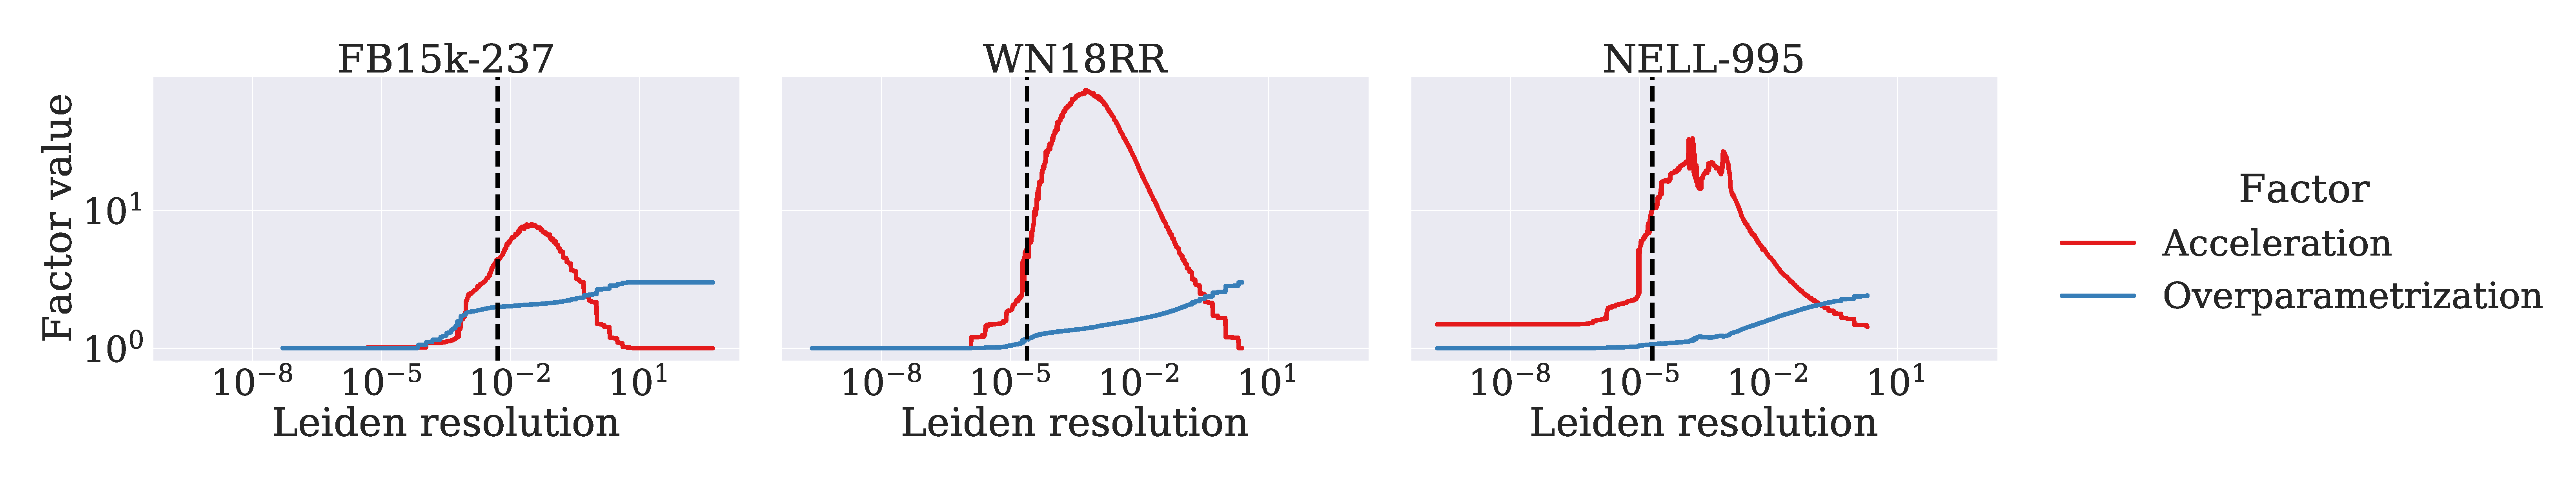
\includegraphics[width=\textwidth]{figures/coins/scalability_leiden_resolution}
\end{center}
\caption[Dependence of time and memory scalability on the value of the resolution hyperparameter of the Leiden community detection algorithm.]{Dependence of time and memory scalability (acceleration and overparametrization factors) on the value of the resolution hyperparameter of the Leiden community detection algorithm. Left to right: different datasets. Chosen hyperparameter values that yielded an optimal balance between scalability and performance for each dataset are annotated via vertical lines.}
\label{fig:scalability_resolution}
\end{figure}

\subsubsection{Performance \& Feasibility}

Tables~\ref{tab:performance_query_answering_mrr} and~\ref{tab:performance_query_answering_q2b} contain our MRR metric query answering results and the comparison with the baselines, where KBGAT baselines were retrieved from~\cite{nathani_learning_2019}, Query2Box metrics were obtained by integrating the base algorithm with our experiment code that has COINs integration deactivated, while for all other models, metrics were calculated by running the implementation provided with~\cite{sun_rotate_2019}\footnote{Available at \url{https://github.com/DeepGraphLearning/KnowledgeGraphEmbedding}}. 
One can observe that, on average, the relative error of the metric to the baseline decreases with the model complexity. This is to be expected, as more representation power means better embedding of the complicated community-node interactions. In a third of the single-hop cases and the majority of multi-hop ones, we even improve upon the baseline results. Refer to Tables~\ref{tab:performance_query_answering} and~\ref{tab:performance_query_answering_2} in Appendix~\ref{sec:appendix_results} for the full details on the query answering metrics. Here, we also provide a decomposition of the ranking scores separately for Step I and II of COINs.

\begin{table}[H]
  \caption[Computed MRR metric of single-hop query answering experiments.]{Computed MRR metric (higher is better) of single-hop query answering experiments for comparison of COINs results to baselines with equal hyperparameters. Values in bold indicate the superiority of COINs, while underlined values have a relative error lower than 10\%.}
  \label{tab:performance_query_answering_mrr}
  \centering
\begin{tabular}{lllllll}
\toprule
Dataset & \multicolumn{2}{l}{FB15k-237} & \multicolumn{2}{l}{WN18RR} & \multicolumn{2}{l}{NELL-995} \\
Value &                 Baseline &                              COINs &                Baseline &                           COINs &                 Baseline &                           COINs \\
Algorithm &                          &                                    &                         &                                 &                          &                                 \\
\midrule
TransE    &              ${{0.218}}$ &            ${{0.132}_{\pm 0.004}}$ &              ${{0.16}}$ &  $\mathbf{{0.278}_{\pm 0.008}}$ &              ${{0.312}}$ &         ${{0.218}_{\pm 0.009}}$ \\
DistMult  &              ${{0.344}}$ &            ${{0.068}_{\pm 0.009}}$ &             ${{0.433}}$ &         ${{0.261}_{\pm 0.071}}$ &              ${{0.395}}$ &         ${{0.127}_{\pm 0.022}}$ \\
ComplEx   &              ${{0.369}}$ &     $\mathbf{{0.431}_{\pm 0.006}}$ &             ${{0.462}}$ &         ${{0.358}_{\pm 0.018}}$ &              ${{0.466}}$ &  $\mathbf{{0.472}_{\pm 0.005}}$ \\
RotatE    &              ${{0.383}}$ &  $\underline{{0.381}_{\pm 0.003}}$ &             ${{0.476}}$ &  $\mathbf{{0.487}_{\pm 0.001}}$ &              ${{0.482}}$ &         ${{0.412}_{\pm 0.018}}$ \\
KBGAT     &              ${{0.518}}$ &            ${{0.245}_{\pm 0.015}}$ &              ${{0.44}}$ &         ${{0.359}_{\pm 0.003}}$ &               ${{0.53}}$ &  $\mathbf{{0.543}_{\pm 0.009}}$ \\
\bottomrule
\end{tabular}
\end{table}

\begin{table}[H]
  \caption[Computed per-query-structure MRR metric of Query2Box query answering experiments.]{Computed per-query-structure MRR metric (higher is better) of Query2Box query answering experiments to compare our results with COINs training and evaluation to baselines with equal hyperparameters. Values in bold indicate the superiority of COINs, while underlined values have a relative error lower than 10\%.}
  \label{tab:performance_query_answering_q2b}
  \centering
    \begin{adjustbox}{width=\textwidth}   
\begin{tabular}{lllllll}
\toprule
Dataset & \multicolumn{2}{l}{FB15k-237} & \multicolumn{2}{l}{WN18RR} & \multicolumn{2}{l}{NELL-995} \\
Value &                 Baseline &                           COINs &                 Baseline &                              COINs &                 Baseline &                             COINs \\
Query &                          &                                 &                          &                                    &                          &                                   \\
\midrule
1p    &  ${{0.176}_{\pm 0.004}}$ &  $\mathbf{{0.276}_{\pm 0.003}}$ &  ${{0.258}_{\pm 0.004}}$ &     $\mathbf{{0.336}_{\pm 0.004}}$ &  ${{0.397}_{\pm 0.005}}$ &    $\mathbf{{0.463}_{\pm 0.009}}$ \\
2p    &  ${{0.027}_{\pm 0.001}}$ &  $\mathbf{{0.124}_{\pm 0.004}}$ &  ${{0.194}_{\pm 0.016}}$ &  $\underline{{0.182}_{\pm 0.026}}$ &  ${{0.516}_{\pm 0.033}}$ &    $\mathbf{{0.524}_{\pm 0.008}}$ \\
3p    &   ${{0.02}_{\pm 0.001}}$ &  $\mathbf{{0.117}_{\pm 0.008}}$ &  ${{0.141}_{\pm 0.009}}$ &      $\mathbf{{0.15}_{\pm 0.044}}$ &  ${{0.086}_{\pm 0.017}}$ &    $\mathbf{{0.172}_{\pm 0.022}}$ \\
2i    &  ${{0.091}_{\pm 0.008}}$ &  $\mathbf{{0.259}_{\pm 0.005}}$ &  ${{0.533}_{\pm 0.016}}$ &     $\mathbf{{0.668}_{\pm 0.025}}$ &  ${{0.313}_{\pm 0.063}}$ &    $\mathbf{{0.315}_{\pm 0.003}}$ \\
3i    &  ${{0.135}_{\pm 0.015}}$ &   $\mathbf{{0.303}_{\pm 0.01}}$ &  ${{0.913}_{\pm 0.151}}$ &         $\mathbf{{1.0}_{\pm 0.0}}$ &  ${{0.421}_{\pm 0.058}}$ &           ${{0.357}_{\pm 0.007}}$ \\
ip    &  ${{0.046}_{\pm 0.005}}$ &  $\mathbf{{0.188}_{\pm 0.008}}$ &  ${{0.329}_{\pm 0.068}}$ &            ${{0.193}_{\pm 0.029}}$ &  ${{0.487}_{\pm 0.029}}$ &           ${{0.278}_{\pm 0.033}}$ \\
pi    &  ${{0.039}_{\pm 0.004}}$ &   $\mathbf{{0.24}_{\pm 0.003}}$ &  ${{0.549}_{\pm 0.008}}$ &     $\mathbf{{0.609}_{\pm 0.075}}$ &  ${{0.585}_{\pm 0.073}}$ &  $\underline{{0.528}_{\pm 0.05}}$ \\
\midrule
Average &  ${{0.154}_{\pm 0.004}}$ &     $\mathbf{{0.261}_{\pm 0.002}}$ &  ${{0.26}_{\pm 0.001}}$ &  $\mathbf{{0.323}_{\pm 0.007}}$ &  ${{0.382}_{\pm 0.004}}$ &  $\mathbf{{0.443}_{\pm 0.004}}$ \\
\bottomrule
\end{tabular}
\end{adjustbox}
\end{table}
To add further context to our obtained results, in Table~\ref{tab:performance_query_answering_related_work} we compared COINs-RotatE's performance to that reported by NodePiece~\cite{galkin_nodepiece_2022} and EARL~\cite{chen_entity-agnostic_2023}, the previously-mentioned related work that also provides scalable model-based solutions at the cost of some performance. From the table, we can infer that in all cases, our approach either beats the baseline or is the one that preserves the most of its strength.

\begin{table}[H]
  \caption[Comparison of Hits@10 and MRR values for query answering between the RotatE baseline, NodePiece, EARL, and COINs.]{Comparison of Hits@10 and MRR values (averaged across seeds) for RotatE query answering between the baseline results in~\cite{sun_rotate_2019}, previous results by the related work NodePiece and EARL provided in~\cite{chen_entity-agnostic_2023}, and this work. The top model is in bold, while the second best is underlined.}
  \label{tab:performance_query_answering_related_work}
  \centering
\begin{tabular}{lrrrr}
\toprule
{} & \multicolumn{2}{l}{Hits@10} & \multicolumn{2}{l}{MRR} \\
Dataset & FB15k-237 & WN18RR & FB15k-237 & WN18RR \\
Value     &           &        &           &        \\
\midrule
Baseline  &     \textbf{0.584} &  \underline{0.538} &  \textbf{0.383} &  \underline{0.476} \\
NodePiece &     0.420 &  0.515 &     0.256 &  0.403 \\
EARL      &     0.501 &  0.527 &     0.310 &  0.440 \\
COINs     &     \underline{0.552} &  \textbf{0.586} &     \underline{0.381} &  \textbf{0.487} \\
\bottomrule
\end{tabular}
% \begin{tabular}{lrrrrrr}
% \toprule
% {} & \multicolumn{2}{l}{MRR} & \multicolumn{2}{l}{Overparametrization} & \multicolumn{2}{l}{Ratio} \\
% Dataset & FB15k-237 & WN18RR &           FB15k-237 & WN18RR & FB15k-237 & WN18RR \\
% Value     &           &        &                     &        &           &        \\
% \midrule
% Baseline  &     0.383 &  0.476 &               1.000 &  1.000 &     0.383 &  0.476 \\
% NodePiece &     0.256 &  0.403 &               1.103 &  1.073 &     0.232 &  0.376 \\
% EARL      &     0.310 &  0.440 &               0.621 &  0.927 &     0.499 &  0.475 \\
% COINs     &     0.381 &  0.487 &               1.995 &  1.165 &     0.191 &  0.418 \\
% \bottomrule
% \end{tabular}
\end{table}

However, a relevant comparison to the baseline is difficult to perform without the aid of an additional scalability-dependent investigation of the applicability of our proposed approach. Unlike~\cite{chen_entity-agnostic_2023}, which only evaluated the ratio of absolute MRR to model size, we believe the more direct and robust scalability comparison is one between the relative error and speed-up. Thus, we plot our values for the relative error in MRR to the baseline against acceleration (reduction in computational complexity) in Figure~\ref{fig:feasibility}. 

\begin{figure}[H]
\begin{center}
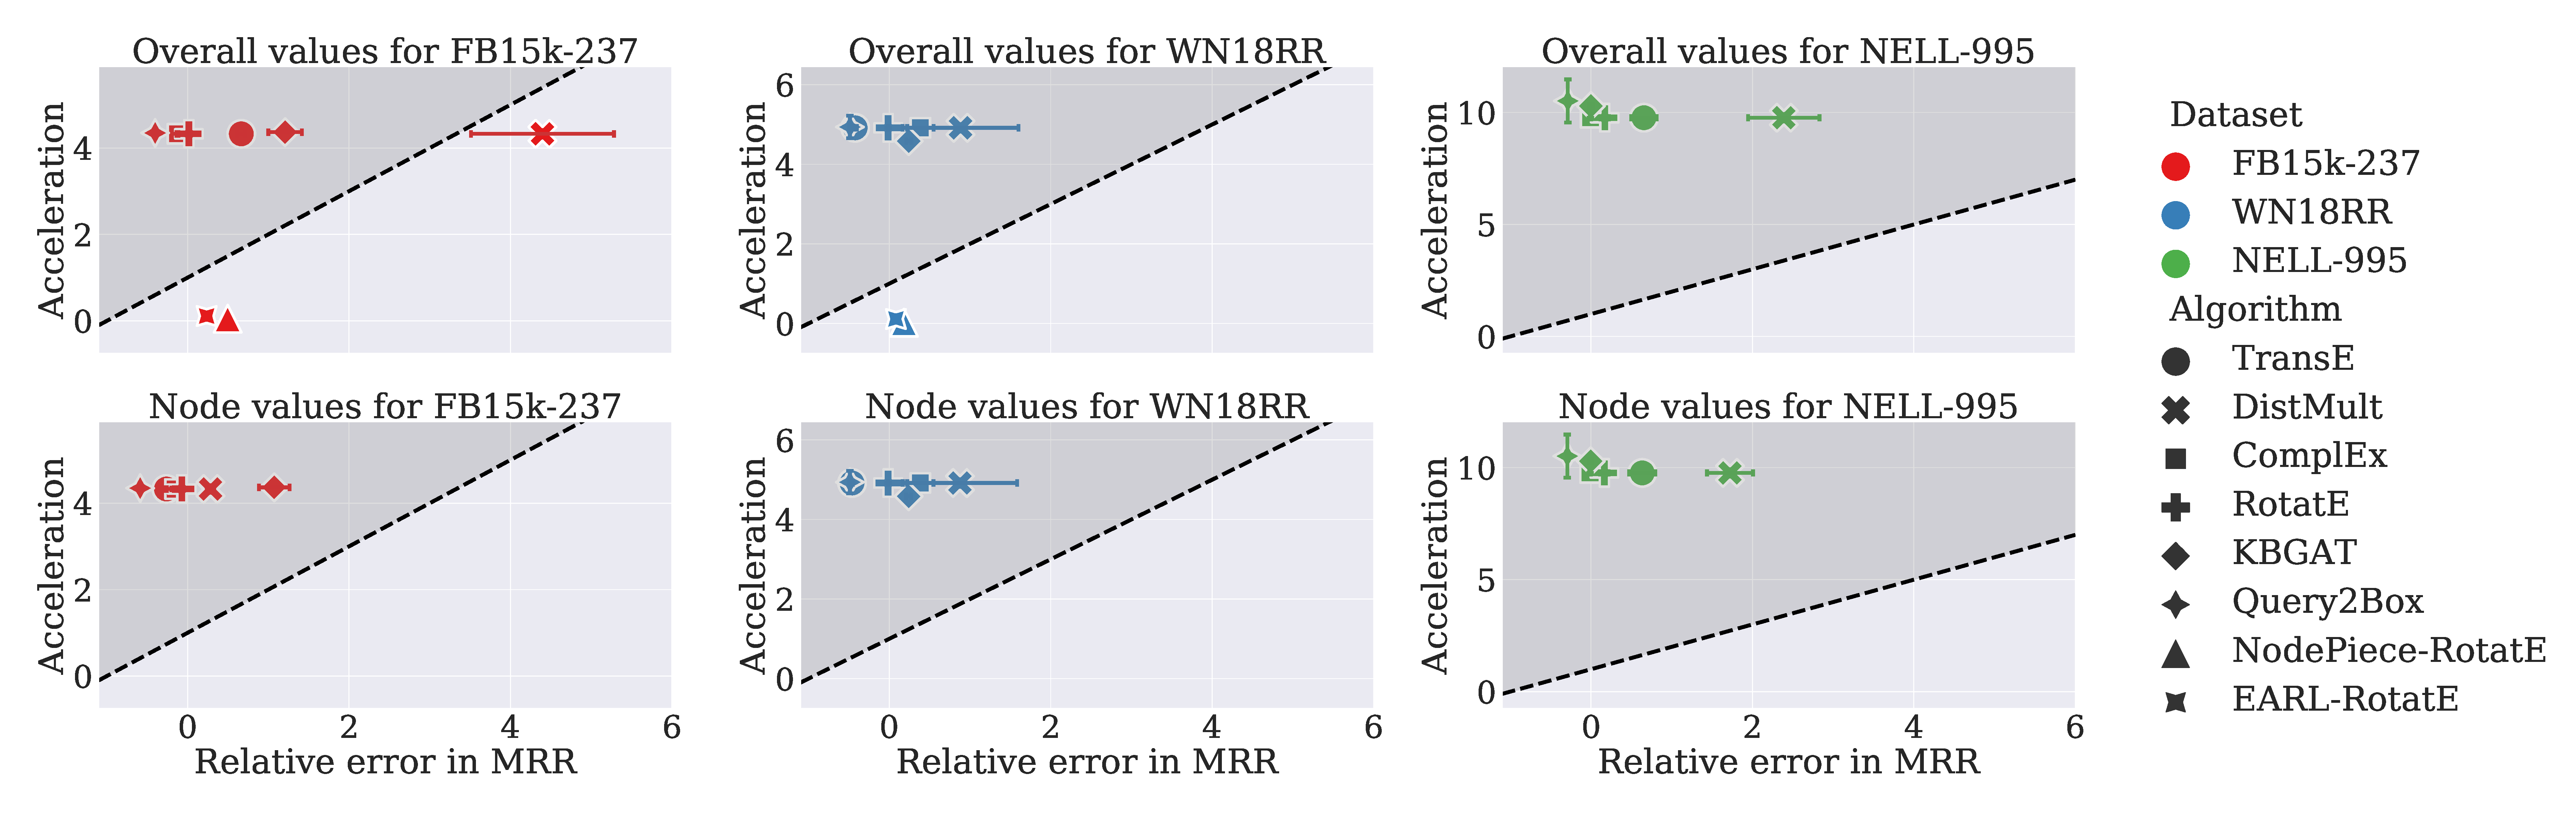
\includegraphics[width=\textwidth]{figures/coins/feasibility_2.pdf}
\end{center}
\caption[Plot of relative error in MRR against acceleration.]{Plot of relative error in MRR (lower is better) against acceleration (higher is better). The feasible region is the one shaded, where the speed-up is at least 100\% larger than the error. Top vs. bottom: values computed from ranks after both steps vs. just the second step of COINs. Removing the error in the ranks caused by the community prediction shows improvement and feasibility of all experiments, explaining the outliers, i.e., some models' inability to learn Freebase communities well. Left to right: different datasets.}
\label{fig:feasibility}
\end{figure}

From the top plots, one can observe that almost all COINs experiments lie deep in the feasible region, with the bottom plots explaining the reason for the few outliers. On the other hand, the NodePiece and EARL baselines are made infeasible by the time-memory trade-off of tokenization.

\subsection{Summary}

In this section, we introduced COINs, a method for accelerating link prediction and query answering models for knowledge graphs, to be applicable even in low computational resource settings. COINs featured a two-step prediction procedure: query answer prediction via community prediction and within-community localization. 
We theoretically and empirically elaborated that the quality of the community structure of the knowledge graph has a broad-reaching influence on the possible scalability improvements provided by our method, as well as its prediction performance compared to baselines. As such, one can conclude that before selecting COINs to accelerate the embedding of a knowledge graph, it is important to study and evaluate its community structure. 

The achieved impressive accuracy and acceleration benefits strongly motivate modeling and predicting over both the community-level coarsened version of a knowledge graph, in addition to the local structures, no matter the task. We would, in such a way, apply both holistic and reductionist techniques to solve a knowledge graph problem, perhaps otherwise computationally intractable.

As relevant future work in scalable knowledge graph reasoning, we propose attempting the integration of COINs with algorithms for general first-order logical knowledge graph query answering, like BetaE~\cite{ren_beta_2020}, and obtaining comparisons to baseline models on larger non-standard knowledge graphs.

\section{Real-world Application: the Monty Knowledge Base}
\label{sec: swisscom}

\subsection{Reporting your knowledge}

Knowledge graphs as a data structure have witnessed numerous applications in a diverse range: journalism, biomedicine, social networks, network security, and, recently, telecommunication. Thus, like many other companies, Swisscom (Switzerland) AG has started building and maintaining its knowledge graph for internal use in the last few years. The end goals include the possibility to analyse telecommunication infrastructure in detail, predict and diagnose possible communication defects that may arise, speed up retrieving customer support information, and many other applications.

Previous research work in the company presented an approach that addressed these prediction challenges; however, experiments showed weak generalization performance for other data sources. Thus, the goal of the study in this section was to present a detailed network-science-based analysis of the properties of this knowledge graph, and more importantly, in what manner they differ most from the properties of publicly available knowledge graph data that can be used for evaluating graph models. The completed results from this study allowed us to perfect the COINs model and apply it successfully to Swisscom's \enquote{Monty} knowledge base. 

Specifically, in this section, we will present a detailed descriptive and comparative knowledge graph analysis methodology that was applied to the company's data, though it is general and detailed so as to be operationalized for broader research purposes. We dissect a knowledge graph with five classes of network science measuring techniques and utilize one-sample goodness of fit and two-sample distribution comparison statistical tests to quantitatively analyze the obtained measures. Before concluding, we present the final link prediction and query answering results on the Monty data. We believe the methodology presented in the following pages has practical research value for constructing all knowledge graph reports. 

\subsection{Related work}
\label{sec:related_work}

As we introduced in Chapter~\ref{chp: background}, the field of \emph{network science} studies methods for analysing specific properties of graph-structured data in order to obtain insight that might be useful for building a predictive model of the target graph/network. 

The book by~\cite{barabasi_network_2016} is a very good introduction to this scientific field, and we adopt the definitions of most graph-related concepts and metrics from this source. Though more dedicated to a random graph theory view of networks,~\cite{lewis_network_2011} also details classical tools.

In~\cite{pinheiro_social_2011}, one can find recommended network science methods for the application of telecom graphs, viewed from the perspective of social networks between customers. On the other hand, we distinguish the experiments by~\cite{kostic_social_2020} as the only recent work found directly applying empirically estimated features from an (again customer-level) telecom network for the churn prediction problem. Though our data structure and task differ, the authors, alike~\cite{pinheiro_social_2011}, support the utility of network connectivity, network clustering, and node importance metrics for the telecom use case, techniques we also employ. We thus hope our study will also similarly empirically motivate and validate similar future work.

\subsection{Methodology}
\label{sec:methodology_swisscom}

As previously introduced, the goal of this project is to dissect and demystify an enormous knowledge graph by producing a detailed report of its properties represented through network features obtained from a thorough unsupervised analysis. Inspired by both classical network science theory and recently proposed methods, we compute 5 classes of network features to form the set of descriptors. For a statistical-test-based comparison between the features as the representation of a graph, we execute the same descriptive procedure for a set of selected public datasets as well. We elaborate on the computational process of the 5 feature classes and statistical comparison in the rest of this section.

\subsubsection{Heterogeneity}

Swisscom's internal knowledge graph is confirmed to be a directed AMHEN. Around 10-50 possible labels for both entities and relations are available. 
 
The presence of type labels for nodes and edges separates AMHENs from simple directed multiplex graphs. To quantify this heterogeneity in detail, we empirically measure the distribution of node types, the distribution of relation types, and the distribution of (head type, relation type, tail type) triplets through appearance frequencies. Note that although the first two distributions can be viewed as marginals of the third, they offer the option for the separation of label distribution comparison. 

To quantify heterogeneity while also acknowledging its dependence on graph structure,~\cite{newman_mixing_2003} proposes the \emph{nominal assortativity} scalar metric for node types. The value is alike a correlation coefficient, negative values indicate frequently changing node types across graph paths, positive values indicate that node types are instead more likely to be preserved across paths, while 0 would be obtained from a uniformly-random label assignment.

\subsubsection{Connectivity}

Quantifying global and local connectivity in relational models is one of the main goals of network science. Connectivity metrics attempt to measure the reachability and neighbourhood sizes of nodes, transitivity of relations, etc. For this work, we considered classically:
\begin{itemize}
    \item Edge density, defined as the ratio of the number of edges to the total possible edges;
    \item Node in-degree and out-degree distributions as value appearance frequencies;
    \item Average path length and graph diameter (maximum path length);
    \item Sizes of weak (undirected) and strong (directed) connected components;
    \item Clustering coefficient for each node, as well as average clustering.
\end{itemize}

Beyond this classical connectivity report, we also compute two scalar metrics quantifying the distribution of connectivity across the graph, used in state-of-the-art generative graph model research for evaluation through similar graph comparison~\cite{krawczuk_gg-gan_2020}. Namely, we implement \emph{degree assortativity proposed} by~\cite{newman_mixing_2003}, as well as the \emph{algebraic connectivity} metric, defined as the second-smallest eigenvalue of the graph Laplacian matrix~\cite{chung_spectral_1996}.

\subsubsection{Importance}

The field of network science also researches how to quantify important/influential entities in a network, by computing some measurable score for vertices according to an underlying theory.

The classical centrality measures are one such class of scores, and for this work, we utilize closeness and betweenness centralities, defining important nodes as those with high reachability or high utility in shortest paths, respectively.

Due to the extreme relevance of the node importance problem, more complex and very prominent algorithms exist, and for this work, we utilize the hub and authority scores of the HITS algorithm~\cite{kleinberg_authoritative_1999} as well as PageRank~\cite{brin_anatomy_1998}.

\subsubsection{Subgraphing}

Given the sheer scale of Swisscom's internal knowledge graph (millions of entities), there is a non-negligible probability of noise and irrelevant information in a graph of that size. Thus, unlike the public data sources, whose size permits a direct computation of metrics belonging to the above three introduced classes, it was decided to structure the analysis pipeline according to domain relevance and applicability. Specifically, we obtain a covering of Swisscom's internal graph through bootstrap sampling of subgraphs. 

The procedure is graphically summarized in Figure~\ref{fig:subgraphing}, while the details are as follows. The full knowledge graph is stored in the form of a Neo4j$\textsuperscript{\textregistered}$ graph-NoSQL database. Domain-relevant queries are first used to extract subgraphs describing part of the networking infrastructure that provides Swisscom services to a customer. When all of the extracted subgraphs (either rooted at customer organizations or customer sites) are merged with a simple union operation, the scale of the covering will at most be equal to the original scale of the graph, as we would prefer.

\begin{figure}[H]
\centering
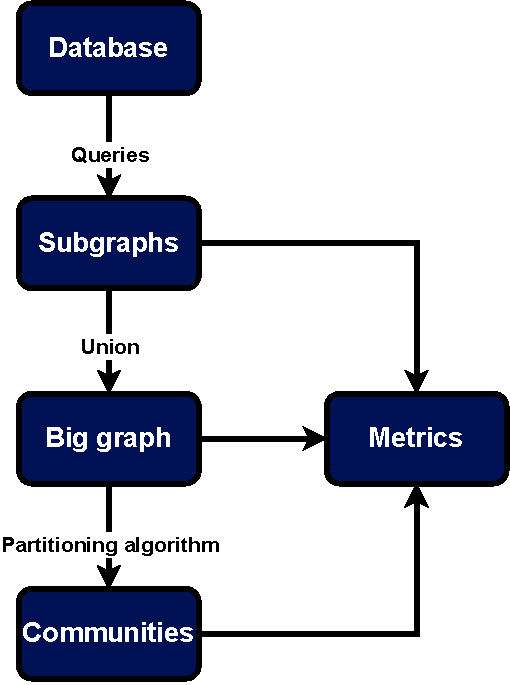
\includegraphics[width=0.35\columnwidth]{figures/swisscom/subgraphing.pdf}
\caption[Monty subgraphing pipeline.]{Monty subgraphing pipeline.}
\label{fig:subgraphing}
\end{figure}

To achieve scalability, the previously developed predictive model utilizes subgraph-based locality of entities and relations to reduce the underlying computational complexity. In order for this approach not to sacrifice prediction accuracy, the subgraphs ideally should be both \emph{representative} samples of the full data, while also sufficiently \emph{informative} such that the subgraph assignment has meaning itself. To help balance these two desirable properties, one can guide the design of the query-based subgraphing by comparing its result to that of a dedicated graph-structure-based partitioning algorithm from the field of community detection. For extracting disjoint communities from the aggregate graph, we employ the state-of-the-art Leiden algorithm~\cite{traag_louvain_2019} for Monty too, while EgoNetSplitter~\cite{epasto_ego-splitting_2017} can efficiently compute a community covering with overlaps.

Due to this design of our subgraphing analysis, we are able to analyze the data from both a macroscopic and microscopic level, by computing the metrics for the big graph, as well as for each subgraph, community, overlap between subgraphs, or overlap between EgoNetSplitter communities, yielding valuable diagnostic opportunities.

The community detection procedures yield useful metrics themselves; we focus on the community size distribution for both the disjoint and overlapping cases, the size distribution of overlapping regions, as well as the Leiden modularity measure of the disjoint partitioning.

Regarding analyzing the subgraph structure of a network, a popular approach is also to estimate the frequencies of all possible tiny non-isomorphic subgraphs, called \emph{motifs}. For this work, we enumerate all of the possible 3 and 4-node directed subgraphs to use as motifs and use the Efficient Sampling Algorithm (ESA), proposed by~\cite{kashtan_efficient_2004}, to estimate their frequency distribution.  

\subsubsection{Summarization}

The field of graph summarization~\cite{liu_graph_2019}, gaining traction in recent years, focuses on obtaining graph \emph{summaries} in order to reduce data volume and storage, speed up graph algorithms and queries, support interactive graph analysis, and eliminate noise. The notion of a graph summary is not well defined; summaries are application dependent and can be defined with respect to various goals, performing data compression in addition to preserving specific structural patterns, preserving answers to graph queries, or maintaining the distributions of graph properties. 

The KGist algorithm~\cite{belth_what_2020} was first considered for the purpose of this study. The method is based on bit-compression techniques, discovering the optimal set of association rules between labels that balance their total description length with the number of relations in the knowledge graph they explain. These metrics are also convenient for comparison of the summary to those of the public graphs.

As preserving query answers and obtaining a summary in the form of a knowledge graph is also desirable for our application, we additionally implement a labeled-graph variation of the graph de-densification algorithm by~\cite{maccioni_scalable_2016}. Using node degrees, the method discovers densely-connected pairs of node sets and rewires these locally-dense regions in a manner that would sparsify the graph while preserving the query result depending on those nodes. The final achieved compression ratio is a useful metric to report. 

Due to the query-relevant nature of our knowledge graphs, we deemed it also profitable to compare datasets w.r.t. their edge-importance-weighted spanning trees. With a simple tree iteration procedure, we compute the distribution of differently labeled paths in the spanning tree as an additional graph summary.

\subsubsection{Statistical Comparison}

\paragraph{Data} For our experiments, in order to serve as baselines for comparisons to our knowledge graph, we considered publicly-available datasets of both a random-graph and designed nature, from many different application domains: the \texttt{redditHyperlinks} dataset of Reddit post relationships from~\cite{kumar_community_2018}, the \texttt{HepPh} citation network of scientific papers in high energy physics and \texttt{cit-Patents} the U.S. patent citation network from~\cite{leskovec_graphs_2005}, the \texttt{ogbl-biokg} knowledge graph of biological entities from the Open Graph Benchmark (OGB) collection (\cite{hu_open_2021}), and finally the set of transport networks of 25 cities collected by~\cite{kujala_collection_2018}.

We also considered the 3 datasets classically used in academic work on knowledge graph reasoning: FB15k-237~\cite{toutanova_observed_2015}, WN18RR~\cite{dettmers_convolutional_2018}, and NELL-995~\cite{xiong_deeppath_2017}.

\paragraph{Tests} After obtaining the value of each metric for each of the public datasets, aggregated Swisscom graph, subgraph, and community, further post-processing of the results, in the form of statistical hypothesis testing, is performed to obtain some directly quantified insight.

First, the main property of each metric, defined as a distribution over nodes, labels, motifs etc., would be whether the distribution has a heavy tail. If the answer is yes, then this implies the full support set of the metric is sufficiently relevant for its value; however, otherwise, as is common for most graphs, the distribution has an exponential decay, implying one can focus on a very small subset of the support. We perform one-sample Kolmogorov-Smirnov tests for the Pareto distribution to investigate this property for every metric and data source.

As mentioned previously, subgraph assignments that yield subgraphs that are representative of the full network are more desirable. Thus, the second one-sample tests we perform are concerned with investigating which metrics are preserved across query-based subgraphs and communities. This is operationalized by running a $\chi^2$-test for the discrete uniform distribution over the metric histogram estimated from its values across the subgraphs. We also test the uniformity of subgraph and community overlaps.

The metric comparison between the Swisscom and other graphs is based on both a simple two-sample t-test and a version of the Maximum Mean Discrepancy (MMD) test as presented in~\cite{gretton_kernel_2012}. Unlike simple mean comparison, MMDs are a two-sample RBF-kernel-based test that is commonly used for graph metric distribution-agnostic comparison in modern research in generative graph models (\cite{you_graphrnn_2018, krawczuk_gg-gan_2020}). The MMD p-value is estimated through bootstrapping. We run the comparison tests between the metric values across subgraphs and communities (and respective overlapping regions) as well, to discover potential equivalence between the two assignments and guide future improvement of the handcrafted database queries.


\subsubsection{Implementation}
The experiments were executed using the Swisscom Big Data (SBD) cloud computing platform, offering access to a distributed file system and computing hardware. CPU execution was feasible, and memory and storage requirements did not exceed 64 GB.

The entire software implementation was performed in the Python 3 programming language. The Neo4j$\textsuperscript{\textregistered}$ Python driver~\cite{neo4j_inc_neo4j_2022} was utilized to run the queries on the database and extract the datasets. Pandas~\cite{mckinney_data_2010} was helpful with its efficient preprocessing operations on tabular data. iGraph~\cite{csardi_igraph_2005} was utilized for the implementation of most of the graph analysis pipeline, while scipy~\cite{virtanen_scipy_2020} implements required operations with sparse matrices and statistical tests. Karate Club~\cite{rozemberczki_karate_2020} yielded easy access to implementations of overlapping community detection algorithms. tensorflowX~\cite{huang_tensorboardx_2022} provided result visualization through an interactive dashboard.

\subsection{Results \& Discussion}
\label{sec:results_swisscom}

We begin by presenting an overall summary of the metric values computed on both the aggregate Swisscom graph and public data. To preserve corporate confidentiality, what follows will only be a textual summary of the relative comparison of the metrics. A global phenomenon we observed is that most of the insights we will report hold for when both organization and site-rooted subgraph queries are used, implying equal diagnostic utility despite unequal measures. 

\subsubsection{Heterogeneity} 
Swisscom, citation and transport graphs have label frequency distributions that are skewed towards at most two very prominent label triplets in the support. Due to the single possible node type in the citation and transport graphs, nominal assortativity is uninformative; however, curiously, it permits only a slightly positive value for our data, implying almost no clear correlation in label assignment, unlike all other public datasets with significantly positive values. We believe this is mainly due to the equal proportion of within-type and between-type relations, as the second most common node triplet is a dominating within-type one.

\subsubsection{Connectivity} 
The edge density in our graph proved to be the lowest out of all datasets, indicating a very sparse, tree-like structure. The patent citation network density is very similar w.r.t. to this metric, though. While no networks had dominated degree distributions, certain entity types in Swisscom's internal knowledge graph have shown to have a slightly higher probability for incoming connections, though this does not seem to hold for outgoing ones, indicating some effect of the schema. 

Both Swisscom and public graphs possess a giant weakly connected component including almost all nodes; however, strong connectivity is not present in the citation networks or Swisscom's graph. Indeed, this is confirmed to be by design, in order to ease specific database query design. This is also reflected in a much smaller average path length and diameter, and these insights motivate the importance of not disregarding the direction of relations for predictive modeling of our data. Another metric most likely influenced by the database design seems to be the average transitivity, which is a couple of orders of magnitude lower for our graph compared to all others. 

The degree assortativity metric also proved a strong discriminator. While it admits a significant negative value for Swisscom's graph and the academic datasets, it varies in the positive range for the citation and transport cases. The spectral algebraic connectivity measure proved uninformative.

\subsubsection{Importance} 
Node importance score distributions also proved to strongly differentiate Swisscom from public data. While transport networks are the only ones with clearly important hub nodes, HITS identified interestingly that authority score instead seems to flow strongly towards certain Swisscom entities, with the WordNet graph being the only other with this property. On the other hand, betweenness centralities and PageRank indicated a slightly less skewed distribution, though they identified common important entities, implying an underlying truth. Closeness centralities proved uninformative.

\subsubsection{Subgraphing} The Leiden algorithm identified a disjoint community structure with strong modularity for Swisscom's network, transport, and WordNet networks. In fact, the Monty KG has an extremely high modularity score of above 0.99, and this was the main motivation to apply a technique like COINs to this data. Though a set of non-trivial assignments was identified for all graphs, as indicated by the balanced community size distributions. EgoNetSplitter, on the other hand, identified a presence of prominent overlapping regions in the Swisscom, citation, and WordNet cases. However, we single out the estimated motif frequency distributions as the most discriminative metrics that seemed to profile all graphs well, as for all graphs, certain different 3 and 4-node structures seem to strongly dominate. 

Figure~\ref{fig:motifs} visualizes the most frequent motifs and their respective frequencies for our knowledge graph, and we observe that neighbourhoods, where a single node has only incoming links from multiple disconnected nodes, are overwhelmingly dominating, indicating an inverted-tree-like structure.

\begin{figure}[ht!]
    \centering
    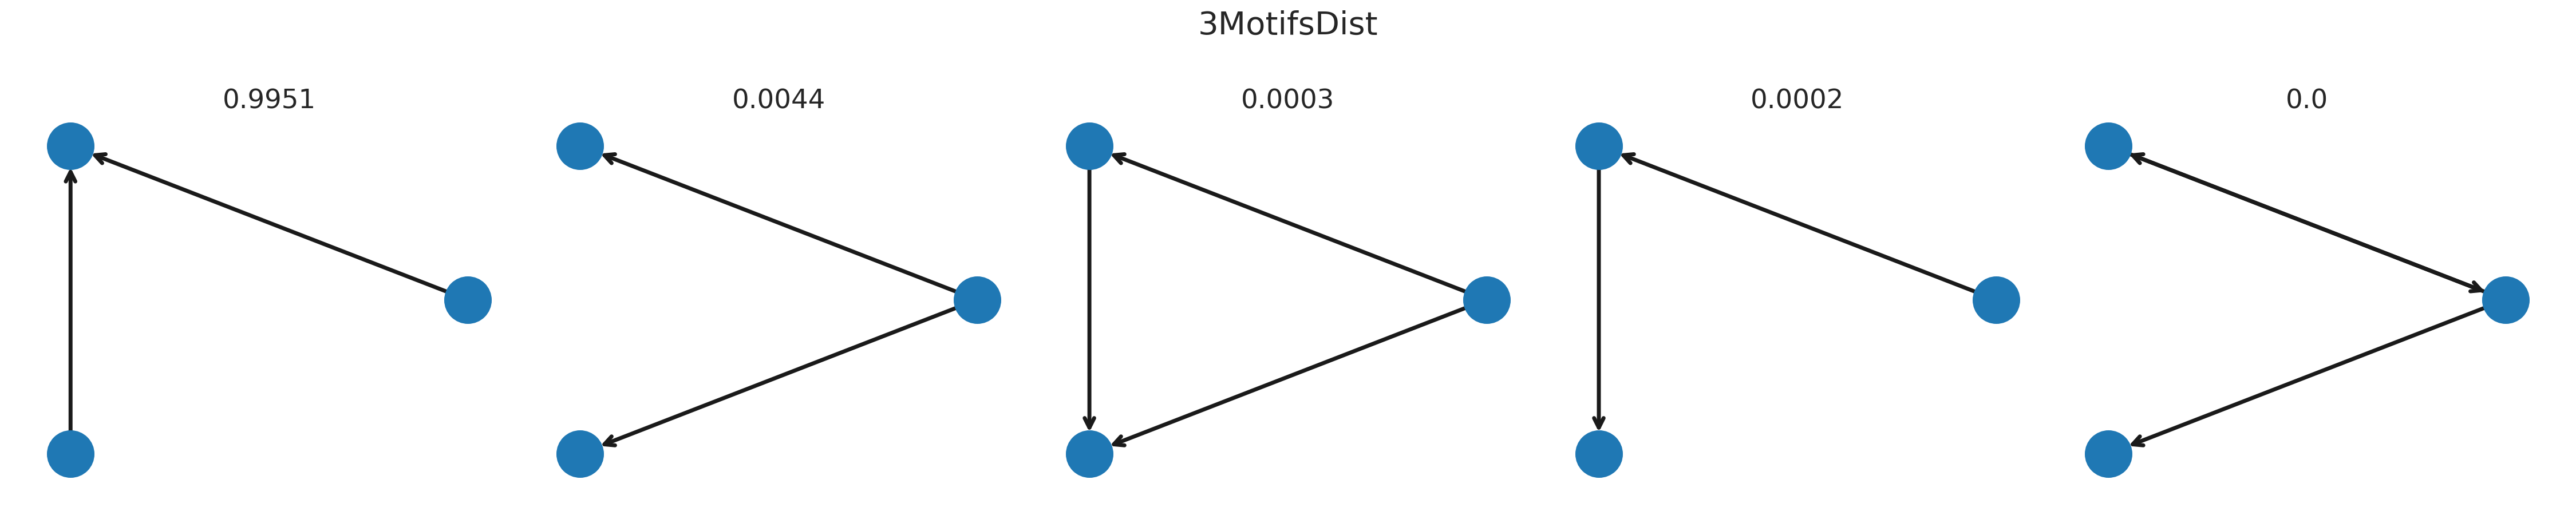
\includegraphics[width=\textwidth]{figures/swisscom/3motifs.png}
    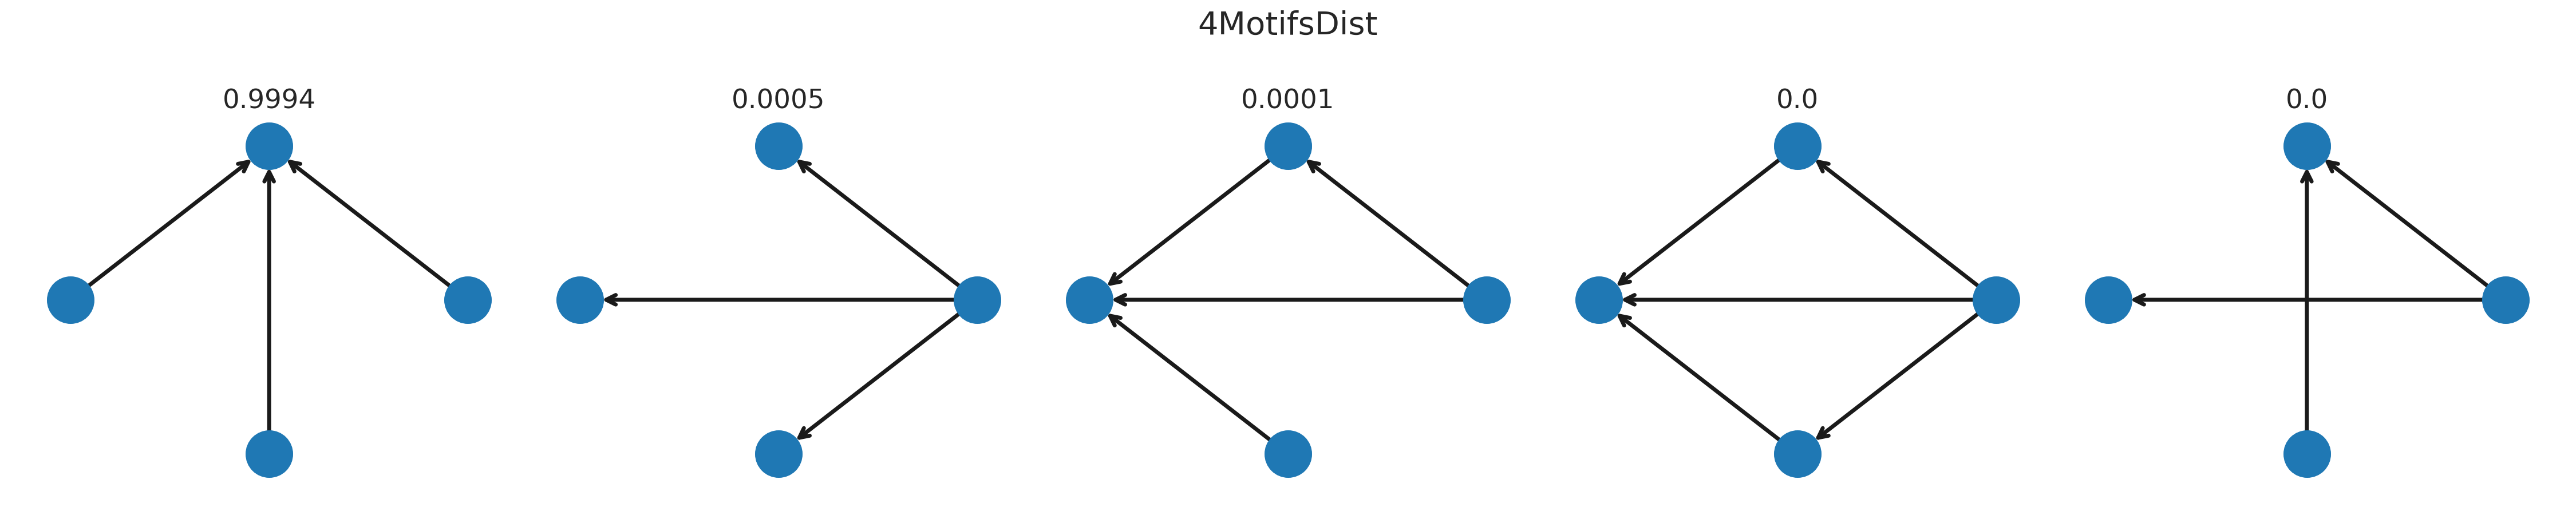
\includegraphics[width=\textwidth]{figures/swisscom/4motifs.png}
    \caption[Most common structural motifs in Swisscom's internal knowledge graph and their frequencies.]{Most common structural motifs in Swisscom's internal knowledge graph and their frequencies. Top vs bottom: 3- vs 4-node motifs. Frequencies decrease from left to right.}
    \label{fig:motifs}
\end{figure}

\subsubsection{Summarization}

The KGist method was able to discover a meaningful summary of our knowledge graph. 10 association rules were returned and achieved a bit compression ratio of 68.45\% while explaining 96.10\% of the edges in the case of organization-rooted subgraph queries, while 7 returned rules achieved a bit compression ratio of 77.14\% while explaining 60.54\% of the edges in the case of site-rooted subgraph queries. %Curiously, the method was not able to return a summary of any transport graph or the patent citation network. 

Unfortunately, the de-densification algorithm was not able to achieve substantial lossless compression, due to the already relatively low edge density of the Swisscom graph. Future work could consider a lossy version of the method or other potentially more powerful approaches. The spanning tree method identified prominent query paths for all graphs, where the distribution skewness for the Swisscom graph is in the medium range.

\subsubsection{Statistical tests}

We move on to presenting the results of our hypothesis testing. Table~\ref{tab:pareto} reports which metrics for which datasets had a statistically significant probability of having a heavy-tailed distribution. We observe that this was proven true for the label distributions in the case of almost all datasets. In addition, interestingly, only for the Swisscom, transport, and citation cases, the motif frequencies are also heavy-tailed. Connected component sizes for a few datasets are significantly Pareto as well, though the Swisscom data is not among these cases.

\begin{table}[hb!]
    \centering
\caption[Pareto goodness of fit tests with p-values above a 0.05 significance threshold for knowledge graph datasets.]{Pareto goodness of fit tests with p-values (4th column) above a 0.05 significance threshold for knowledge graph datasets. For these metric distributions, we also report the estimated value of the polynomial degree parameter of the Pareto distribution (3rd column). For the 25 transport graphs, only the city with the highest p-value w.r.t. a metric is included for brevity.}
\label{tab:pareto}
\begin{adjustbox}{width=0.75\columnwidth}
\begin{tabular}{llrr}
\toprule
             &                   &  $\alpha$ &  $p$ \\
Metric & Dataset &              &               \\
\midrule
WCC & transport-antofagasta &       0.0000 &        1.0000 \\
OverlappingRegionSizeDist & transport-bordeaux &       0.0000 &        1.0000 \\
RelationDist & redditHyperlinks &       0.0000 &        1.0000 \\
LabelInteractionDist & redditHyperlinks &       0.0000 &        1.0000 \\
NodeTypeDist & HepPh &       0.0000 &        1.0000 \\
RelationDist & HepPh &       0.0000 &        1.0000 \\
LabelInteractionDist & HepPh &       0.0000 &        1.0000 \\
NodeTypeDist & cit-Patents &       0.0000 &        1.0000 \\
RelationDist & cit-Patents &       0.0000 &        1.0000 \\
LabelInteractionDist & cit-Patents &       0.0000 &        1.0000 \\
             & transport-adelaide &       0.4572 &        1.0000 \\
NodeTypeDist & fb15k-237 &       0.0000 &        1.0000 \\
SCC & transport-palermo &       0.0000 &        1.0000 \\
RelationDist & transport-adelaide &       0.4572 &        1.0000 \\
NodeTypeDist & redditHyperlinks &       0.0000 &        1.0000 \\
             & transport-adelaide &       0.0000 &        1.0000 \\
             & ogbl-biokg &       2.2765 &        0.8730 \\
3MotifsDist & swisscom-big-orgs &       0.3522 &        0.7714 \\
             & swisscom-big-sites &       0.5061 &        0.7714 \\
             & transport-adelaide &       0.4454 &        0.7714 \\
WCC & fb15k-237 &       0.6184 &        0.4740 \\
             & ogbl-biokg &       0.5062 &        0.4740 \\
NodeTypeDist & wn18rr &       0.2397 &        0.3571 \\
3MotifsDist & cit-Patents &       0.6474 &        0.2286 \\
             & HepPh &       0.2362 &        0.0794 \\
NodeTypeDist & swisscom-big-sites &       0.2205 &        0.0530 \\
DisjointCommunitySizeDist & fb15k-237 &       0.8213 &        0.0314 \\
4MotifsDist & transport-belfast &       0.6811 &        0.0207 \\
NodeTypeDist & swisscom-big-orgs &       0.1042 &        0.0186 \\
\bottomrule
\end{tabular}
\end{adjustbox}
\end{table}

Regarding the tests for metric uniformity across subgraphs, communities, and respective overlaps of the Swisscom data, the result is extremely positive, as all metric histograms appeared uniform with high statistical significance. 

Table~\ref{tab:t} reports which metrics for which public datasets had a statistically significant probability of having equal distribution means with the metrics computed over Swisscom data. If for more than one public graph the p-value of the comparison was significant, we report the one with the largest p-value. 

Although for most metrics listed in this table, we discussed that for our graph, they are relatively different from what we observed for the public data, the t-test signals that there is at least no reason to reject the hypothesis of equal means. The negative sign of the statistic's values also supports our previous observations of commonly lower metric values for our graph. The results interestingly imply that at least some equivalence can be made between the Swisscom and public data w.r.t. the motif frequency, connected component size, or label distributions. The patent citation, WordNet, and transport networks stand out as examples.

On the other hand, Table~\ref{tab:mmd} reports which metrics had a statistically significant probability of having equal distributions according to the Maximum Mean Discrepancy test. These results disprove a couple of the previous similarity insights; however, the label distribution similarity significance prevails, and now we also obtain the insight that the Swisscom graph's motif distribution is actually more similar to the NELL and transport graphs. The MMD test is more strict, but also more accurate, so we will assign greater value to these results compared to the Student tests.

\begin{table}[ht!]
    \centering
    \caption[Two-sample t-tests for metric distribution mean comparison between Swisscom and public data.]{Two-sample t-tests for metric distribution mean comparison between Swisscom and public data with p-values (5th column) above a 0.01 significance threshold. For these metric distribution pairs, we also report the estimated value of the t statistic (4th column). Only the public dataset with the highest p-value w.r.t. a metric is included for brevity.}
    \label{tab:t}
\begin{adjustbox}{width=0.8\columnwidth}
\begin{tabular}{lllrr}
\toprule
                   &                   &          &   $t$ &  $p$ \\
Dataset \#1 & Dataset \#2 & Metric &         &              \\
\midrule
swisscom-big-orgs & cit-Patents & 3MotifsDist &  0.0000 &       1.0000 \\
                   &                   & SCC &  0.0000 &       1.0000 \\
swisscom-big-sites & cit-Patents & SCC &  0.0000 &       1.0000 \\
swisscom-big-orgs & transport-belfast & 4MotifsDist & -0.0000 &       1.0000 \\
swisscom-big-sites & cit-Patents & 3MotifsDist &  0.0000 &       1.0000 \\
                   & transport-dublin & 4MotifsDist &  0.0000 &       1.0000 \\
                   & redditHyperlinks & WCC &  0.0784 &       0.9375 \\
                   & ogbl-biokg & BetweennessCentrality & -0.1708 &       0.8644 \\
                   & fb15k-237 & AuthorityScore & -0.2311 &       0.8172 \\
                   & wn18rr & NodeTypeDist & -0.3648 &       0.7263 \\
swisscom-big-orgs & redditHyperlinks & DisjointCommunitySizeDist & -0.3668 &       0.7138 \\
                   & wn18rr & RelationDist & -0.4231 &       0.6761 \\
swisscom-big-sites & ogbl-biokg & OverlappingCommunitySizeDist &  0.4250 &       0.6708 \\
swisscom-big-orgs & wn18rr & NodeTypeDist & -0.4403 &       0.6706 \\
                   & redditHyperlinks & WCC & -0.4682 &       0.6397 \\
swisscom-big-sites & wn18rr & RelationDist & -0.4920 &       0.6285 \\
swisscom-big-orgs & transport-helsinki & LabelInteractionDist & -0.8000 &       0.4645 \\
swisscom-big-sites & transport-helsinki & LabelInteractionDist & -0.8104 &       0.4611 \\
                   & redditHyperlinks & DisjointCommunitySizeDist &  0.7935 &       0.4276 \\
swisscom-big-orgs & cit-Patents & AuthorityScore & -0.8501 &       0.3953 \\
                   &                   & HubScore & -0.8828 &       0.3773 \\
                   & wn18rr & SpanningTreePathDist & -1.0341 &       0.3011 \\
swisscom-big-sites & cit-Patents & SpanningTreePathDist &  1.4331 &       0.1519 \\
                   & transport-belfast & HubScore & -1.4705 &       0.1416 \\
\bottomrule
\end{tabular}
\end{adjustbox}
\end{table}

\begin{table}[ht!]
    \centering
        \caption[MMD tests for metric distribution comparison between Swisscom and public data.]{MMD tests for metric distribution comparison between Swisscom and public data with p-values (5th column) above a 0.01 significance threshold. For these metric distribution pairs, we also report the estimated value of the MMD statistic (4th column). Only the public dataset with the highest p-value w.r.t. a metric is included for brevity.}
    \label{tab:mmd}
\begin{adjustbox}{width=0.8\columnwidth}
\begin{tabular}{lllrr}
\toprule
                   &           &                           &    MMD &  $p$ \\
Dataset \#1 & Dataset \#2 & Metric &        &            \\
\midrule
swisscom-big-orgs & transport-palermo & SCC & 0.0000 &     1.0000 \\
swisscom-big-sites & transport-antofagasta & 3MotifsDist & 0.0911 &     1.0000 \\
                   & transport-palermo & SCC & 0.0000 &     1.0000 \\
                   & transport-sydney & RelationDist & 0.0890 &     0.9500 \\
                   &           & LabelInteractionDist & 0.0902 &     0.8600 \\
swisscom-big-orgs & wn18rr & LabelInteractionDist & 0.0411 &     0.5800 \\
                   &           & NodeTypeDist & 0.1872 &     0.5400 \\
                   & transport-canberra & RelationDist & 0.3026 &     0.5100 \\
                   & nell-995 & 3MotifsDist & 0.1687 &     0.4300 \\
swisscom-big-sites & transport-sydney & NodeTypeDist & 1.4733 &     0.3300 \\
                   &           & WCC & 0.0420 &     0.2500 \\
swisscom-big-orgs & ogbl-biokg & WCC & 0.1441 &     0.2400 \\
swisscom-big-sites & nell-995 & 4MotifsDist & 0.0494 &     0.2300 \\
swisscom-big-orgs & fb15k-237 & 4MotifsDist & 0.1081 &     0.0900 \\
swisscom-big-sites & fb15k-237 & DisjointCommunitySizeDist & 0.1601 &     0.0200 \\
\bottomrule
\end{tabular}
\end{adjustbox}
\end{table}

Finally, no metrics had a statistically significant probability of having equal histogram means or low MMD across both query-based subgraphs and communities. Interestingly, both the query-based subgraphs and communities yield a highly representative partitioning of the big graph, though each is of its own nature. 

Respective overlapping regions, on the other hand, curiously had significant Student and MMD p-values only in the customer-site case, w.r.t. connected component size and graph diameter.

\subsubsection{Reasoning experiments for Monty}

To finalize the result discussion, we provide in Table~\ref{tab:swisscom_coins} the achieved knowledge graph reasoning results after applying COINs to Monty data. Query answering experiments were focused on single-hop queries only, as a proof of concept. A train-validation-test data split of the Monty data was obtained through uniform stratified sampling, while COIN's hyperparameters were set to the same values as for the WN18RR dataset (this is supported by the previous discussion indicating the similarity between these two graphs). 

We observe how the Swisscom metrics are in about the same range as those achieved on the academic data, implying we have obtained an approach that successfully generalizes. In addition, when estimating the scalability benefits of COINs for Monty, we obtained that \emph{728.7} times fewer query embeddings were computed during evaluation, and \emph{228.36} times less training memory was used in comparison to the baseline, proving that COINs' benefits can indeed scale with graph size.

\begin{table}[!ht]
    \centering
    \caption[Link prediction and query answering metrics after applying COINs models to the Swisscom dataset.]{Link prediction and query answering metrics after applying COINs models to the Swisscom dataset (higher is better), with a comparison to top results of the same models on the academic knowledge graphs. The best value per metric is highlighted in bold.}
    \label{tab:swisscom_coins}
    % \begin{adjustbox}{width=0.75\columnwidth}
    \begin{tabular}{llrrrrrr}
    \toprule
         Dataset & Model & F1 & AP & Hits@1 & Hits@3 & Hits@10 & MRR \\
    \midrule
         FB15k-237 & COINs-Best & 0.938 & 0.900 & 0.333 & 0.477 & 0.626 & 0.431 \\
         WN18RR & COINs-Best & 0.917 & 0.871 & 0.436 & 0.510 & 0.586 & 0.487 \\
         NELL-995 & COINs-Best & 0.965 & 0.963 & 0.445 & 0.633 & 0.740 & 0.555 \\
         \midrule
         Monty & COINs-TransE & 0.875 & \textbf{0.749} & 0.048 & 0.159 & 0.334 & 0.138 \\
         Monty & COINs-DistMult & \textbf{0.893} & 0.740 & 0.165 & 0.241 & 0.343 & 0.223 \\
         Monty & COINs-ComplEx & 0.889 & 0.736 & \textbf{0.428} & \textbf{0.446} & \textbf{0.459} & \textbf{0.441} \\
         Monty & COINs-RotatE & 0.719 & 0.554 & \textbf{0.428} & 0.444 & 0.452 & 0.439 \\
    \bottomrule
    \end{tabular}
    % \end{adjustbox}
\end{table}

\subsection{Summary}
\label{sec:summary}

In this section, we have presented a detailed descriptive and comparative knowledge graph analysis methodology that was applied for data collected for diagnostic purposes in the telecommunications sector, though it is general and detailed so as to be operationalized for broader research purposes. 

We dissected a knowledge graph with five classes of network science measuring techniques and utilized one-sample goodness of fit and two-sample distribution comparison statistical tests to quantitatively analyze the obtained measures.

The obtained results yielded a plethora of non-trivial insights into our data source, from which the main conclusion one can extract is that the Swisscom data is more similar to knowledge graph datasets traditionally constructed for learning knowledge graph reasoning than to random graphs like citation networks. This paves the way for future research at the company in improving the current query answering model trained on this data. Before us is thus another instance of a mixture between holistic and reductionist views of a knowledge graph that could not provide the same value on their own.

\chapter{Scalable Graph Generation}
\label{chp: generation}

\section{Geometric Graph Generation with the Chinese Restaurant Process}
\label{sec: gggcrp}

The task of generative models is to learn from empirical observations how to model distributions and/or sample from them, and research into Generative Adversarial Networks (GANs) has yielded very successful solutions to the problem. Geometric graph generation is a way of representing graphs spatially, usually with node embeddings and assigning edges according to closeness w.r.t. a distance metric in embedding space. These techniques carry potential to transform a wide range of application domains, as with this approach, deep graph generative models are able to represent graphs in a more compact form. Research of this type is still ongoing to attempt to answer remaining questions posed by some experimental results. Namely, what is the best approach to further improve the scalability of the current state-of-the-art graph generation models, as the current best performance drops for larger graphs, while preserving their high expressive power and exchangeability?

In this section, we will present an approach to integrating permutation-invariant community-detection-based metrics into a Chinese Restaurant Process to perform exchangeable sequence modeling for graph generation. This approach, when integrated into the current-best graph GAN, yielded a new variation of the model, named GGG-CRP. Current results will be shown as comparable to the base model in the wake of strong resource reduction, demonstrating promise for improvement in immediate future work.

\subsection{Motivation}

The task of generative models is to learn from empirical observations how to
model distributions and/or sample from them. Research into Generative Adversarial Networks (GANs) has yielded very successful solutions to the problem, and results were already incredible and human-like with audio-visual data \cite{karras_analyzing_2020}. However, graphs are a challenging variant; they are \emph{discrete} structures with potential for highly complex relational structure. 
Earlier studies on GANs for graph generation (\cite{bojchevski_netgan_2018, de_cao_molgan_2018}) yielded models with relatively good performance, though they tended to memorize training data in the lack of domain-specific rewards or specific data properties. Therefore, to mitigate this issue of limited model applicability, more generalizable approaches started to gain popularity, such as geometric techniques.

\emph{Geometric} graph generation is a way of representing graphs spatially, usually with node embeddings and assigning edges according to closeness w.r.t. a distance metric in embedding space. With this approach, deep graph generative models represent graphs in a more manageable form and carry potential to transform a wide range of application domains: computational chemistry (novel drug discovery), electrical circuit modelling and design (complete automation of this process), computational biology (novel synthetic proteins), etc.

As noted by \cite{krawczuk_gg-gan_2020}, a graph generator $g$ should possess 4 desirable properties:
\begin{enumerate}[1.]
\item \emph{Expressive power} - $g$ should be able to model local and global dependencies between nodes and graph edges, going beyond simple degree statistics and learning structural features and motifs;
\item \emph{Scalability} - $g$ should have efficient computation, its tractability should be invariant to graph size;
\item \emph{Isomorphism consistency} - alike e.g., convolutional networks, $g$ should respect the permutation symmetry of its domain of graphs \cite{bronstein_geometric_2021}, i.e., assign isomorphic graphs the same probability, a property also referred to as exchangeability/permutation equivariance;
\item \emph{Novelty} - $g$ should produce non-isomorphic graphs that are similar to (but not necessarily in) the training set.
\end{enumerate}

To satisfy these properties, \cite{krawczuk_gg-gan_2020} proposed such an exchangeable geometric generator called GG-GAN. Surprisingly, classical geometric approaches have so far found limited adoption in the context of deep generative graph models. GG-GAN precisely bridges this gap, showing how deep geometric approaches can perform well. It sheds light on some basic limits and challenges of geometric graph generators and solves these problems with a novel latent state, while retaining consistency through equivariance.

This research is still ongoing, to attempt to answer remaining questions posed by some experiment results, namely: what is the best approach to further improve the scalability of the GG-GAN graph generation model, as the current best performance drops for larger graphs, while preserving its high expressive power and exchangeability. The work for this project consisted of focusing on the implementation of one of the proposed approaches: exchangeable sequence modeling with Chinese Restaurant Processes (CRPs), assisted by overlap-agnostic community detection, to incur the distribution modelling benefits of autoregressive models without sacrificing generation novelty and diversity. 

% In the following Section \ref{sec:background} we will present the properties of CRPs and graph community detection, as well as in short the GG-GAN model, in order to assist the later explanation of the changes by focusing only on the relevant targets. In Section \ref{sec:methodology} we will present our approach for permutation-equivariant community-agnostic graph modelling and generation. Section \ref{sec:results} discusses the first experimental results of the research, while the final Section \ref{sec:conclusion} gives a few concluding remarks.

\subsection{Background}
\label{sec:background_gggcrp}

\subsubsection{Preliminaries}

\begin{definition}
    Given a set of samples $\mathcal{D}=\{(\mathbf{X}_i)\}_{i=1}^{N}$, with $\mathbf{X}_i \in \mathbb{R}^F$, a \emph{generative model} $\mathcal{M}=\{f,g\}$ models sample likelihoods as $\mathbb{P}(\mathbf{X} \in \mathcal{D})=\sigma(f(\mathbf{X}))$ with $f: \mathbb{R}^F \times \to \mathbb{R}$, and generates new samples from the dataset as $\hat{\mathbf{X}}=g(Z)$, from sampled latent noise $Z\in\mathbb{R}^D$ with $g_n:\mathbb{R}^D \to \mathbb{R}^F$. The optimal sampler $g$ is found most commonly by minimizing the expected \emph{negative log-likelihood loss}:
    \begin{equation}
        g^*=\argmin_{g}{\mathbb{E}_{\mathcal{D},Z}[-\log{\mathbb{P}(g(Z) \in \mathcal{D})}]}=\argmin_{g}{\mathbb{E}_{\mathcal{D},Z}[-\log{\sigma(f(g(Z)))}]}
    \end{equation}
\end{definition}

Wasserstein GANs are one of the most powerful generative models.

\begin{definition}
   A Wasserstein Generative Adversarial Network (WGAN) \cite{arjovsky_wasserstein_2017} is a generative model $\mathcal{M}=\{d,g\}$, where both $d$ and $g$ are parametrized as neural networks whose parameters are optimized with min-max optimization of the \emph{Wasserstein distance}:
   $$g^*=\argmin_{g}\max_{\text{1-Lipschitz } d}{\mathbb{E}_{\mathbf{X}\in\mathcal{D},Z}[d(\mathbf{X})-d(g(Z))]},$$
   where the primal variable $g$ is referred to as the \emph{generator} and the dual variable $d$ as the \emph{discriminator}. The 1-Lipschitz constraint for the dual variable is enforced artificially through various empirical techniques.
\end{definition}

\begin{definition}
Given the dataset $\mathcal{D}=\{(n_i,\mathbf{X}_i,A_i,\mathbf{y}_i)\}_{i=1}^{N}$, where $n_i$ is the number of nodes in the $i$-th graph sample, $\mathbf{X}_i \in \mathbb{R}^{n_i \times F_V}$ is the matrix of node features, $A_i \in \{0,1,\dots,|R|\}^{n_i \times n_i}$ is the graph adjacency matrix enhanced with edge label information and $\mathbf{y}_i \in \mathbb{R}^{F_G}$ is the vector of global graph features, \emph{dense graph generation} involves learning a generative model $\mathcal{M}=\{f,g\}$ for this specific sample structure. Formally, $\mathcal{M}$ samples graph sizes $n$, models the likelihood as $\mathbb{P}((\mathbf{X},A,\mathbf{y}) \in \mathcal{D})=\sigma(f_n(\mathbf{X},A,\mathbf{y}))$ with $f_n: \mathbb{R}^{n \times F_V} \times \{0,1,\dots,|R|\}^{n \times n} \times \mathbb{R}^{F_G} \to \mathbb{R}$, and generates new samples from the dataset as $(\hat{\mathbf{X}},\hat{A},\hat{\mathbf{y}})=g_n(Z)$, from sampled latent noise $Z\in\mathbb{R}^D$ with $g_n:\mathbb{R}^D \to \mathbb{R}^{n \times F_V} \times \{0,1,\dots,|R|\}^{n \times n} \times \mathbb{R}^{F_G}$.
\end{definition}

\subsubsection{Geometric Graph Generation with GG-GAN}
Two main issues plague current top non-equivariant graph generators: 
\begin{itemize}
\item Even though they can approximate any distribution arbitrarily up to their constraints, they can \emph{waste a significant portion of capacity} modeling graphs that are isomorphic to each other - the isomorphism consistency property guaranteed by models like GG-GAN is a solution;
\item In general, they are not \emph{injective} functions; they have no guarantee that two random latent vectors will not be mapped to the same graph (\emph{collisions}) - GG-GAN's novel generator latent state helps to mitigate this problem, though not yet completely.  
\end{itemize}

GG-GAN \cite{krawczuk_gg-gan_2020} is an LP-penalty Wasserstein GAN \cite{gulrajani_improved_2017} with a permutation-equivariant generator and discriminator duo. GG-GAN's generator $g$ conceptually consists of three serially-connected parts; its architecture is visually represented in Figure \ref{fig:gg_gan_g}. The \emph{root} constructs the node latent state used as initialization from the generator. Here the novel alternative to the standard Gaussian latent state, $Z_i \in \mathbb{R}^{n_i \times D} \sim N(0,I)$, is the idea to leave $P<D$ of the latent dimensions as \emph{fixed}, while the remaining a part of a single random context vector $z \in \mathbb{R}^{D-P}$. This fixed point set $\Phi_i \in \mathbb{R}^{n_i \times P}$ could either be a fully-learnable parameter set or, e.g., chosen fixed points in a higher-dimensional binary or spherical embedding space. With this setup, the collision avoidance task is addressed together with the instability issues of GAN training at the same time. 

The \emph{trunk} is a permutation-equivariant function $t: \mathbb{R}^D \to \mathbb{R}^{F}$ that computes a further embedding of the node set, $X_i \in \mathbb{R}^{n_i \times F}$, which is given to the \emph{edge readout} function $r: \mathbb{R}^{n_i \times F} \to \mathbb{R}^{n_i \times n_i}$ to transform it into a probabilistic adjacency matrix. The final adjacency output $A_i$ is obtained by sampling the sigmoid-activated readout values as Bernoulli random variables. A \emph{node readout} function with a similar structure can generate node features $\mathbf{X}_i$ if required. To guarantee equivariance, both the trunk and readouts utilize provably-equivariant deep layers such as (multi-head) attention or point-wise MLPs. To allow the generator \emph{adaptability} to variable graph sizes $n_i$, this single graph meta-variable is modeled and sampled as a categorical random variable whose probability mass function and range are estimated from the dataset.

The discriminator $d$, represented in Figure \ref{fig:gg_gan_d}, passes each graph input to two heads, whose output features are concatenated before a MLP classifier: one is a known permutation-equivariant Message Passing Neural Network (MPNN) from previous work, while the other computes classical handcrafted graph features in a differentiable manner - to preserve both universality and exchangeability of the discriminator.

\begin{figure}
    \centering
    \begin{minipage}{0.475\textwidth}
    \centering
    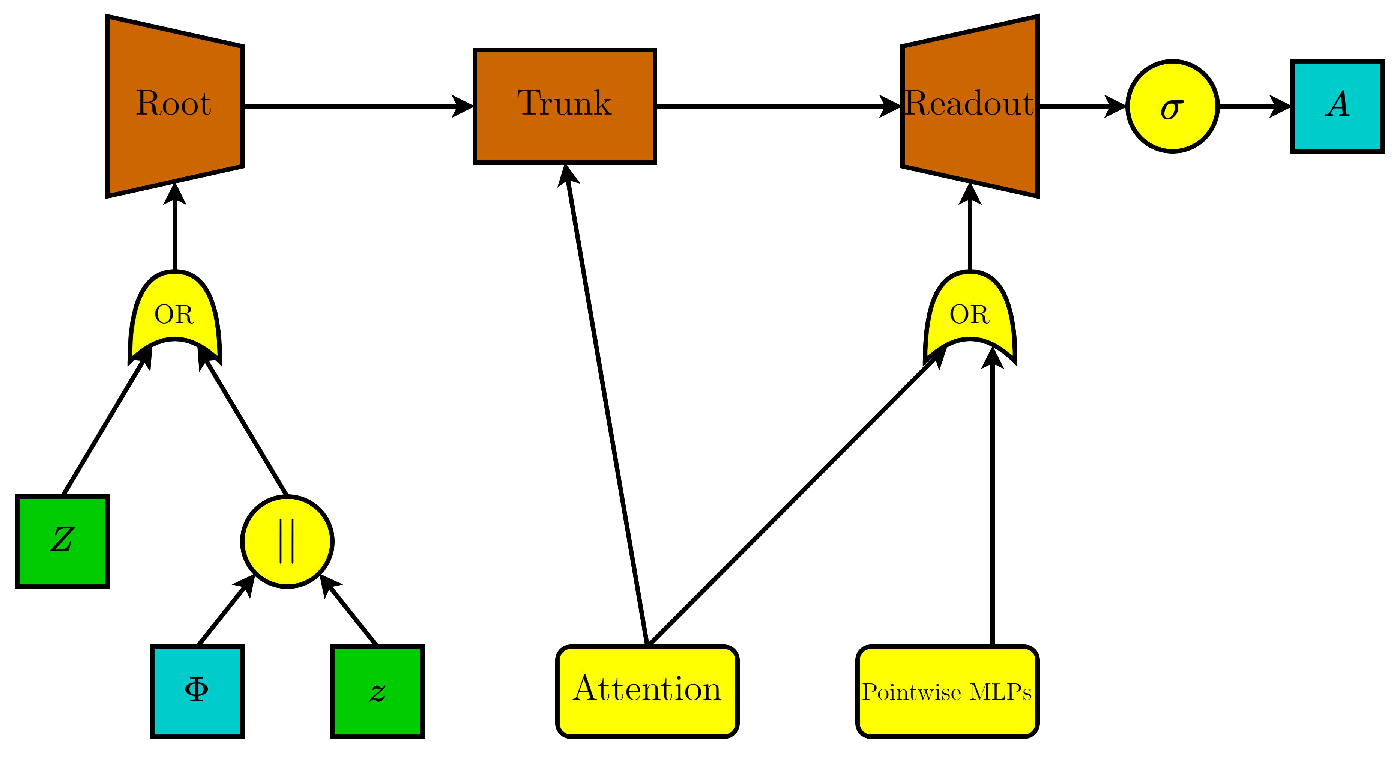
\includegraphics[width=\textwidth]{figures/gggcrp/gg_gan_g.pdf}
    \caption{GG-GAN generator architecture.}
    \label{fig:gg_gan_g}    
    \end{minipage}
    \hfill
    \begin{minipage}{0.475\textwidth}
    \centering
    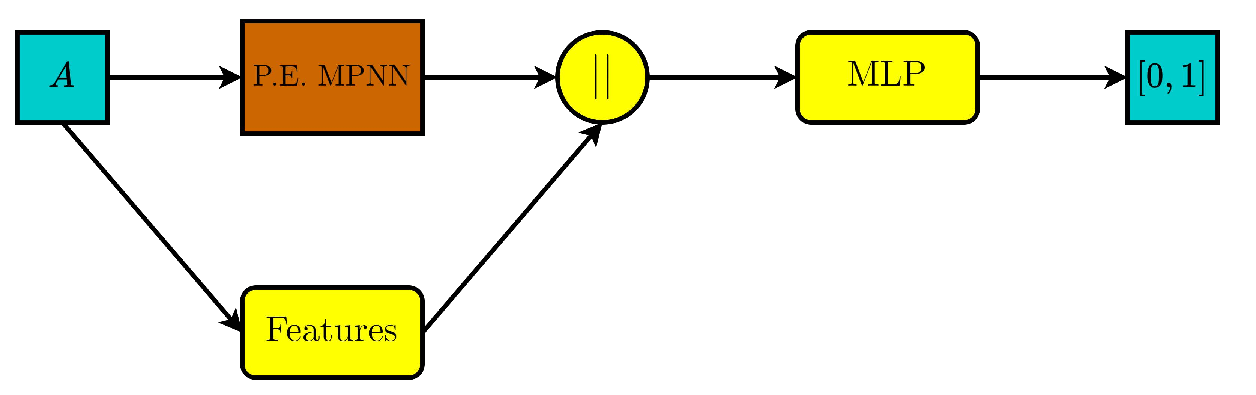
\includegraphics[width=\textwidth]{figures/gggcrp/gg_gan_d.pdf}
    \caption{GG-GAN discriminator architecture.}
    \label{fig:gg_gan_d}    
    \end{minipage}
\end{figure}

\subsubsection{Chinese Restaurant Processes}
In probability theory, the Chinese Restaurant Process (CRP) is a discrete-time stochastic process, analogous to a customer-table assignment sequence in a restaurant \cite{aldous_exchangeability_1985}. Imagine a restaurant with an infinite number of circular tables, each with infinite capacity. Each customer chooses to either sit at an occupied table with a probability proportional to the number of customers already there or at an unoccupied table. At time $n$, $n$ customers have been partitioned among $k \leq n$ tables (or \emph{blocks} of the partition).

\begin{definition}
    Formally, given $n \in \mathbb{N}$, at time $n$ the \emph{Chinese Restaurant Process} is the collection of random variables $\pmb{X}=\{X_i\}_{i=1}^{n}$ whose support is $\mathcal{P}_n$, the set of all integer partitions of the number $n$, i.e. $\sum_{i=1}^{n}{X_i}=n$. The CRP's probability transition function is given by: 
\begin{align*}
&\mathbb{P}\{\pmb{X}=\{x_i\}_{i=1}^{n}|\pmb{X}=\{y_i\}_{i=1}^{n-1}\} = \\
&= \begin{cases} 
\frac{y_k}{n}, & x_n=0, x_k = y_k+1 \wedge \forall j \neq k, x_j=y_j \\
\frac{1}{n}, & x_n = 1 \wedge \forall j \leq n-1, x_j=y_j \\
0, & \text{otherwise} \end{cases}
\end{align*}
\end{definition}

Based on this and using the ratio definition and chain rule of probability, it can be shown that the CRP's probability mass function can be given by: 
$$\mathbb{P}\{\pmb{X}=\{x_i\}_{i=1}^{n}\} = \frac{1}{n!}\prod_{i=1}^{n}{(x_i - 1)!}$$

So we observe the main benefit of the CRP, the realizations of this process are exchangeable, meaning the order in which the \enquote{customers sit} does not affect the probability of the final distribution, as due to the permutation-invariance of products, it only depends on the block size values and not their order. This is a very useful property, as it leads to the possibility of building an autoregressive variant of the GG-GAN generator that will remain exchangeable, by envisioning graph nodes as the \enquote{customers} and generalizing the CRP block (\enquote{table}) assignment to be agnostic to graph structure (instead of purely stochastic).

\subsubsection{Overlapping Community Detection}
Both historic and more recent overview studies (\cite{xie_overlapping_2013, li_deeper_2018, liu_deep_2020, vieira_comparative_2020}) suggest that matrix factorization, heuristic, and deep model approaches, all exhibit satisfactory overlapping community detection performance. These studies evaluate the different methods on known benchmark datasets for overlapping community detection, such as the LFR benchmark \cite{lancichinetti_benchmarks_2009} and dedicated appropriate scoring metrics.

Research into deep Graph Neural Network (GNN) overlapping community classifiers is known to be very limited, but the few published models already display excellent results \cite{jia_communitygan_2019, wang_unifying_2020}. However, their main downside is that they are classification models that need to be pre-trained with at least some known community labels for the dataset, i.e., all are semi-supervised approaches. In addition, recently \cite{huang_combining_2020} has pointed out that due to their message passing nature, community detection GNNs are not unlike the classic label propagation algorithm in terms of distributing and assigning labels, in this case, community membership, to nodes. Indeed, they show that with certain techniques, label propagation can achieve comparable results to GNNs.

The state-of-the-art algorithm for disjoint community detection remains the Leiden algorithm \cite{traag_louvain_2019}, as we discussed previously as well. An heuristic-based approach, it is an improvement of the classic Louvain algorithm. It provides very useful guarantees that Louvain was discovered to not: no detected community is formed from more than one connected component, and itself is not a disconnected component of the full graph. It has been proven to be the current best due to these properties and its excellent scalability to very large graphs. For overlap-agnostic heuristic algorithms, many proven options exist: EgoNetSplitter \cite{epasto_ego-splitting_2017}, LEMON \cite{li_local_2018}, LPANNI \cite{lu_lpanni_2019}, CPPR \cite{gao_overlapping_2021}, etc. The benefits of heuristic-based algorithms are their high efficiency and direct output of the communities, though detection accuracy is not always guaranteed.

Matrix factorization methods usually display higher accuracy and always support overlaps, though they suffer from higher computation costs, and since the partitioning is most often represented as a real-valued matrix, discretization is usually required to obtain the community membership. Best-performing models of this type are BigClam \cite{yang_overlapping_2013}, MNMF \cite{wang_community_2017}, DANMF \cite{ye_deep_2018}. To perform the discretization required for the output of these models, one can, e.g., employ the background edge probability threshold proposed in \cite{jia_communitygan_2019}. An interesting case is the DNMF method by \cite{ye_discrete_2019}, as it solves an additional optimization problem to find the optimal discretization of the original decomposed matrix output, therefore not requiring introduction of implicit bias through a separate discretization, though by doing so, incurring higher computational cost.

Interestingly, some authors have successfully employed reinforcement learning for this task. \cite{zhang_mixed_2017} and \cite{bello-orgaz_multi-objective_2018} have developed evolutionary algorithms for overlapping community detection, while \cite{wang_effective_2021} instead formulated the problem in a game theory setting. 

As hinted in the previous section, we require a CRP block assignment that will be agnostic to graph structure. As (overlapping) communities represent a natural \enquote{ground-truth} partitioning of a graph, we believe they are the most appropriate to be used as CRP blocks. After careful consideration of their properties and code availability, it was decided to validate only most of the heuristic- and matrix-factorization-based algorithms for this project. Credit to \cite{csardi_igraph_2006, rozemberczki_karate_2020, li_local_2018, janchevski_dnmf-python_2022} for the implementations.

\subsection{Methodology}
\label{sec:methodology_gggcrp}

In the following text, we will present our approach on how to integrate permutation-invariant community-based metrics into a CRP to perform exchangeable sequence modelling for graph generation. This approach, when integrated into GG-GAN, yields a new variation of the model, tentatively named GGG-CRP. 

\textbf{Notes on notation:} $\mathbb{N}_{m} = \{1,\dots,m\}$ will denote the set of the first $m$ natural numbers; the index $i$ will denote a batch sample (graph); $j$ will denote the \emph{cardinality} of an overlapping region, defined as the number of different communities that are overlapping to form the region; $k$ will denote a community and $l$ will denote a single node.

\subsubsection{Data augmentation}
The first step required for the new graph distribution modeling approach for GG-GAN is to run a selected overlapping community detection algorithm on each graph in the dataset. The dataset for GG-GAN is represented as the set $\mathcal{D} = \{(\mathbf{X}_i, A_i)\}_{i=1}^{N}$, where $x_i$ are the node feature vectors, $A_i$ are the graph adjacency matrices, i.e., we do not consider global graph features. We condense and represent the output of the graph partitioning algorithm through the matrix $M_i = \text{OCD}(A_i) \in \{0, 1\}^{n_i \times k_i}$, which from here on shall be referred to as the \emph{membership matrix}. $k_i \leq n_i$ is the number of detected communities and $M_{i,l,k}=1$ denotes that in graph $i$, node $l$ is a member of community $k$.

The membership matrix in the general case has two natural constraints: all communities must be non-empty, $\forall k \in \mathbb{N}_{k_i}, (M^T_i \cdot 1_{n_i})_k > 0$; all nodes must be assigned $\forall l \in \mathbb{N}_{n_i}, (M_i \cdot 1_{k_i})_l > 0$. In the special case of disjoint communities, this property is represented by $M_i$ satisfying additionally: $M_i \cdot 1_{k_i} = 1_{n_i}$.

During model training, as will also be evident from later explanations, the new generator would require only the membership matrix as additional input from the data. However, for graph sampling during evaluation, novel node permutation-invariant graph meta-statistics are required as a replacement for it. One is the \emph{overlapping region size matrix} $O_i \in (\mathbb{N}\cup\{0\})^{k_i \times k_i}$, where $O_{i,j,k}$ counts how many nodes of overlapping region cardinality $j$ are members of community $k$ for graph $i$. It can be computed directly from the membership matrix:
$$O_i = \text{OneHotEncode}(M_i \cdot 1_{k_i})^T \cdot M_i$$
The \emph{community size vector} $c_i \in \mathbb{N}^{k_i}$ counting the number of nodes assigned to each community can also easily be computed: $$c_i = M^T_i \cdot 1_{n_i} = O_i^T \cdot 1_{k_i}$$
In the special case of disjoint communities, we have only cardinality-1 nodes (each nodes belongs to only one community): $$O_{i,1}=c_i, O_{i,2}=\dots=O_{i,k_i}=0_{k_i}$$.
The final augmented dataset is thus the collection: $$\mathcal{D}^* = \{(\mathbf{X}_i, A_i, k_i, c_i, O_i, M_i)\}_{i=1}^{B}$$

\subsubsection{Modeling and sampling of permutation-invariant graph meta-variables}
Recall that in order for GG-GAN's generator to be robust to variation in graph size in a dataset, the graph size is estimated and sampled as a categorical random variable. We can now naturally improve the adaptability of the model by estimating and sampling the newly available community-related statistics as well.

\paragraph{Estimated distribution}

Instead of just the maximum graph size, the full list of estimated order statistics is now:
\begin{itemize}
\item Maximum graph size: $n_{\max}=\max_{i=1}^{N}{n_i}$
\item Maximum number of communities: $$k_{\max}=\max_{i=1}^{N}{k_i}$$
\item Maximum community size: $$c_{\max}=\max_{i=1}^{N}\max_{k=1}^{k_i}{c_{i,k}}$$
\item Maximum overlapping region size: $$o_{\max}=\max_{i=1}^{N}\max_{j=1}^{k_i}\max_{k=1}^{k_i}{O_{i,j,k}}$$
\end{itemize}

The full list of random variables and vectors that need to be modeled and sampled for GGG-CRP is:

\begin{itemize}
\item Number of nodes / graph size: $n \in \mathbb{N}_{n_{\max}}$
\item Number of overlapping region cardinalities: $$K^c \in \mathbb{N}_{k_{\max}}$$
\item Number of nodes per cardinality: $$N^c \in (\mathbb{N}_{n_{\max}} \cup \{0\})^{k_{\max}}$$
\item Number of communities per cardinality: $$K \in \mathbb{N}_{k_{\max}}^{k_{\max}}$$
\item Overlapping region size: $$O \in (\mathbb{N}_{o_{\max}} \cup \{0\})^{k_{\max} \times k_{\max}}$$
\end{itemize}

The collection of graph meta-variables is thus $(N, K^c, N^c, K, O)$ and to generalize GG-GAN's approach, is modeled with a jointly-categorical distribution $\mathcal{F}$ whose probabilities are estimated from the data as relative frequencies. In this manner, no independence assumptions are introduced, though for larger graphs, due to potential memory issues, a sparse implementation of the estimated probability tensors is recommended.

\paragraph{Graph meta-variable sampling}

The pseudocode of the full meta-variable sampling algorithm for GGG-CRP is given in Algorithm \ref{algorithm:graph_meta_sampling}. Note: a subscripted $\mathcal{F}$ in the pseudocode denotes a marginalized version of the joint meta-variable distribution.
\begin{algorithm}[t!]
\caption{Graph meta-variable sampling}
\label{algorithm:graph_meta_sampling}
\begin{algorithmic}
\STATE{\textbf{sample} number of nodes and cardinalities: $n_i, K^c_i \sim \hat{\mathcal{F}}_{N,K^c}$}
\STATE{\textbf{sample} partition of nodes across cardinalities: $N^c_i \sim \text{PartitionDistribution}(n_i, K^c_i, \hat{\mathcal{F}}_{n_i, K^c_i, N^c})$}
\FOR{cardinality $j \gets 1$ to $k_{\max}$}
\STATE{\textbf{sample} number of communities for cardinality: $K_{i,j} \sim \hat{\mathcal{F}}_{n_i, K^c_i, N^c_{i,j}, K_j}$}
\STATE{\textbf{sample} overlapping region sizes: $O_{i,j} \sim \text{PartitionDistribution}(j \cdot N^c_{i,j}, K_{i,j}, \hat{\mathcal{F}}_{n_i, K^c_i, N^c_{i,j}, K_{i,j}, O_j})$}
\STATE{\textbf{assign} nodes with cardinality: $\mathcal{N}_{i,j} = \left\{\sum_{k=1}^{j-1}{N^c_{i,k}},\dots,\sum_{k=1}^{j}{N^c_{i,k}}\right\} \subseteq \mathbb{N}_{n_{\max}}$}
\STATE{\textbf{sample} membership: $M_{i,\mathcal{N}_{i,j}} \sim \text{BipartiteGraphDistribution}(j \cdot 1_{N^c_{i,j}},O_{i,j})$}
\ENDFOR
\STATE{\textbf{compute} number of communities: $K_i = \max_{j=1}^{k_{\max}}{K_{i, j}}$}
\STATE{\textbf{compute} community sizes: $C_i = O^T_i \cdot 1_{k_{\max}}$}
\RETURN{$n_i, K_i, C_i, O_i, M_i$}
\end{algorithmic}
\end{algorithm} 

$\text{PartitionDistribution}(n,m,p)$ denotes the distribution over partitions of the integer $n$ into exactly $m$ parts, where $p$ is a probability distribution over the possible sizes of the parts in $\mathbb{N}_{n}$. \cite{fristedt_structure_1993} gives an algorithm that performs partition sampling, with the guarantee of the least amount of rejections and $\text{PartitionDistribution}(n,m,\text{Uniform}) \sim \text{Uniform}$, i.e., it is also provably unbiased in the case of uniform part size probabilities. Unfortunately, in the general scenario for our model, $p$ is not uniform if we wish to be robust to any region size distribution. Therefore, instead of this algorithm, we employed general rejection sampling. Further work might show how to extend Fristedt's guarantees to general part size distributions.
    
$\text{BipartiteGraphDistribution}(a,b)$ denotes the uniform distribution over all bipartite graphs with the two degree sequences $a$ and $b$. We can observe that each node-chunk membership matrix indeed can be viewed as a bipartite graph, where the other graph meta-variables represent its node and chunk degree sequences. The membership matrix of each graph has to be randomly sampled, as there are usually multiple valid solutions to the assignment problem. 
    
To sample a uniform random bipartite graph with degree constraints, one can employ methods such as the Configuration Model \cite{newman_structure_2003} or the Havel-Hakimi algorithm \cite{hakimi_realizability_1963, kleitman_algorithms_1973}. Another idea is to sample the assignment based on node-chunk distance in the root latent space. Formally, if the root's fixed latent point set is $\Phi_i \in \mathbb{R}^{n_i \times P}$, we can also assign a fixed latent representation for each community: $\Phi^c_i \in \mathbb{R}^{k_i \times P}$. If $\ell: \mathbb{R}^{P} \times \mathbb{R}^{P} \to \mathbb{R}$ is an appropriate distance metric for the latent space, then the assignment probabilities can be computed as: $$\mathbb{P}\{M_{i,l,k}=1\}=\frac{\ell(\Phi_{i,l},\Phi^c_{i,k})}{\sum_{k' \in \mathbb{N}_{k_{\max}}}{\ell(\Phi_{i,l},\Phi^c_{i,k'})}}$$

\subsubsection{Exchangeable graph generation agnostic to community structure}
As stated above, to utilize the benefits of exchangeable autoregressive models, instead of single-shot graph generation, we will employ a block-by-block CRP-inspired technique. The generation will thus take place in multiple \emph{rounds}, such that in each round the edges incident to the nodes in one block will be generated. In this manner, the generated graph sequentially grows to its target size.

The first crucial decision is thus how to perform the block assignment of nodes, and as also stated above, the computed overlapping communities will serve the role of CRP blocks. Formally, given graph meta-data $(n_i, K_i, C_i, O_i, M_i)$, computed from the dataset or sampled, we compute the community sets $\mathcal{C}_{i,1},\dots,\mathcal{C}_{i,K_i} \subseteq \mathbb{N}_{n_i}$ according to the given membership matrix: $$\forall k \in \mathbb{N}_{K_i},\mathcal{C}_{i,k}=\{l \in \mathbb{N}_{n_i}| M_{i,l,k} = 1\}$$

GGG-CRP's generator now computes the root for each block/round separately, by collecting the latent points according to the block assignment:
\begin{align*}
&\forall k \in \mathbb{N}_{k_{\max}}, \forall l \in \mathbb{N}_{c_{\max}}, \\
R_{i,l}^{(k)} &= \begin{cases} z_i||\Phi_{i,\mathcal{C}_{i,k,l}}, & l \leq C_{i,k} \\ 0, & \text{otherwise} \end{cases}
\end{align*}
The autoregressive architecture of GGG-CRP is facilitated through a new edge readout function $r'$, modified to accept the discriminator features of the current graph in addition to the trunk's output for the current block. 

With this setup in mind, GGG-CRP's generator pipeline design is given in Algorithm \ref{algorithm:crp_generator}. The main scalability benefits of autoregressive generation techniques for graphs lie in the reduction in memory complexity, as with this setup, only one CRP block of a graph is processed at a time.

\begin{algorithm}[H]
\caption{GGG-CRP graph generation}
\label{algorithm:crp_generator}
\begin{algorithmic}
\STATE{\textbf{initialize} first graph: $A_{i}^{(1)} = r(t(R_{i}^{(1)}))$}
\STATE{\textbf{initialize} prior: $X_{i}^{(1)} = R_{i}^{(1)}$}
\FOR{round $k \gets 2$ to $k_{\max}$}
\STATE{\textbf{update} graph: $A_{i}^{(k)} = r'(t(R_{i}^{(k)}),X_{i}^{(k-1)})$}
\STATE{\textbf{update} prior: $X_{i}^{(k)} = d_f(A_{i}^{(k)})$}
\ENDFOR
\RETURN{final generated graph $A_i = A_{i}^{(k_{\max})}$}
\end{algorithmic}
\end{algorithm} 

Regarding scaling up performance to larger graphs, observe that if there were overlapping nodes present, each would have been added in the generated graph with exactly as many copies as its number of communities. This is intentional and we believe natural, as nodes belonging to multiple communities should have their representation refined multiple times as well. Due to this decision, however, all but the last-added copy of these nodes needs to be pruned from the final readout output, as well as the non-trailing zero-padding entries.

In addition, to mitigate a discovered vanishing gradient issue with the CRP generator (expected due to the now recurrent architecture), a BatchNorm layer was added after the trunk output in each round, and the readout attention layers were configured to use ReLU activation instead of Softmax.

\subsubsection{Multi-level connectivity regularization}
With the computation of community-based metadata for the graphs, we obtain a unique opportunity to add a special type of regularization for the generator. Namely, one can compute a coarsening of each graph, the connectivity between communities as nodes themselves. The generator would be evaluated now with an additional Wasserstein score added to the discriminator loss, computed based on this higher-level connectivity, with a dedicated regularization parameter. 

Formally, let $(\mathbf{X}_i, A_i, k_i, c_i, O_i, M_i)$ be a graph sample from the augmented dataset or sampled from the generator. One can compute the community-level features $\mathbf{X}^C_i \in \mathbb{R}^{k_i \times F}$ and (multiplex) edges $A^C_i \in (\mathbb{N} \cup \{0\})^{k_i \times k_i}$ in the following manner: $$\mathbf{X}^C_i = (M^T_i \cdot \mathbf{X}_i) \oslash c_i, A^C_i = M^T_i \cdot A_i \cdot M_i$$
The coarser graph sample is thus the collection $(\mathbf{X}^C_i, A^c_i, k_i)$.

We stress that the proper validation of this score's regularization parameter is crucial, since if the discriminator weighs too strongly the coarser connectivity, it will underfit as the coarse-to-fine graph mapping is not injective, leaving the generator a chance to fool the discriminator. This can also be mitigated by enriching the coarse graph with further features as edge weights, to reduce collisions.

% This idea can be generalized through iteration of the community detection and connectivity recomputation to produce coarser and coarser graph representations in a hierarchical fashion, each level contributing a regularizer. We predict this modification of the loss function will improve the scalability of the model to very large graphs.

\subsubsection{Experiments}

To preserve the relevance of comparisons, the experimental setup for evaluating GGG-CRP was planned as identical to the one for the original GG-GAN.

The list of datasets chosen for evaluation consisted of: the QM9 dataset \cite{de_cao_molgan_2018}, the HouseFloorplan dataset \cite{nauata_house-gan_2020}, the Chordal9 dataset \cite{mckay_chordal_2020}, and the Community20 dataset \cite{niu_permutation_2020}.

Expressive power was evaluated by comparing real and generated graphs w.r.t. 5 desired graph metrics of increasing complexity: node degree distribution, clustering coefficient, cycle distribution, algebraic connectivity and degree assortativity. The comparison was performed through the Maximum Mean Discrepancy (MMD) scores of \cite{you_graphrnn_2018} computed between the generated and real metric distributions.

Generation novelty was evaluated by studying the number of different isomorphism classes generated, only considering those that differ from those in the training set.

\subsection{Results \& Discussion}
\label{sec:results_gggcrp}

Table \ref{tab:expressive_power} contains the MMD scores obtained by the current best-performing model configurations of each type. Unfortunately, we observe that even though GGG-CRP currently, for most metrics, can provide a comparable performance to GG-GAN for each dataset, a select few graph features prove difficult to train. A special case is perhaps the HouseFloorplan dataset, for which we obtain impressive performance with GGG-CRP, while GG-GAN could not scale to it at all.

\begin{table}[H]
\centering
\caption[Comparison of expressive power between GG-GAN and GGG-CRP.]{Comparison of expressive power between GG-GAN and GGG-CRP. Lower MMD scores denote better performance.}
\label{tab:expressive_power}
% \setlength{\arrayrulewidth}{0.5mm}
%\adjustbox{width=0.475\textwidth}{
\begin{tabular}{llrr}
\toprule
Dataset & Metric MMD & GG-GAN & GG-CRP \\
\midrule
QM9 & Degree & 0.0038 & 0.1079\\
QM9 & Cluster & 0.0341 & 0.0234 \\
QM9 & Cycle & 0.0248 & 0.2587 \\
QM9 & AC & 0.0206 & 0.9121 \\
QM9 & DA & 0.0252 & 0.0896 \\
Community20 & Degree & 0.0023 & 0.0110 \\
Community20 & Cluster & 0.4359 & 0.4061 \\
Community20 & Cycle & 6.7E-6 & 1.4186E-5 \\
Community20 & AC & 0.0785 & 0.0861 \\
Community20 & DA & 0.1312 & 0.4718 \\
Chordal9 & Degree & 0.0281 & 0.0203 \\
Chordal9 & Cluster & 0.0130 & 0.0360 \\
Chordal9 & Cycle & 0.0455 & 0.0092 \\
Chordal9 & AC & 0.0322 & 0.9223 \\
Chordal9 & DA & 0.0690 & 0.0733 \\
HouseFloorplan & Degree & / & 0.0033 \\
HouseFloorplan & Cluster & / & 0.0369 \\
HouseFloorplan & Cycle & / & 0.0129 \\
HouseFloorplan & AC & / & 7.3910E-6 \\
HouseFloorplan & DA & / & 0.0204 \\
\bottomrule
\end{tabular}
%}
\end{table}

We observe this visually as well: Figures \labelcref{fig:qm9,fig:community_20,fig:chordal9,fig:house} present visualizations of a set of sampled graphs from the CRP generator, as well as the real and fake degree and cycle distributions for each dataset. We observe that the HouseFloorplan distribution is learned well; however, a persistent lack of a few connecting edges can be observed for the other three datasets.

\begin{figure}
    \centering
    \begin{minipage}{0.475\textwidth}
    \centering
    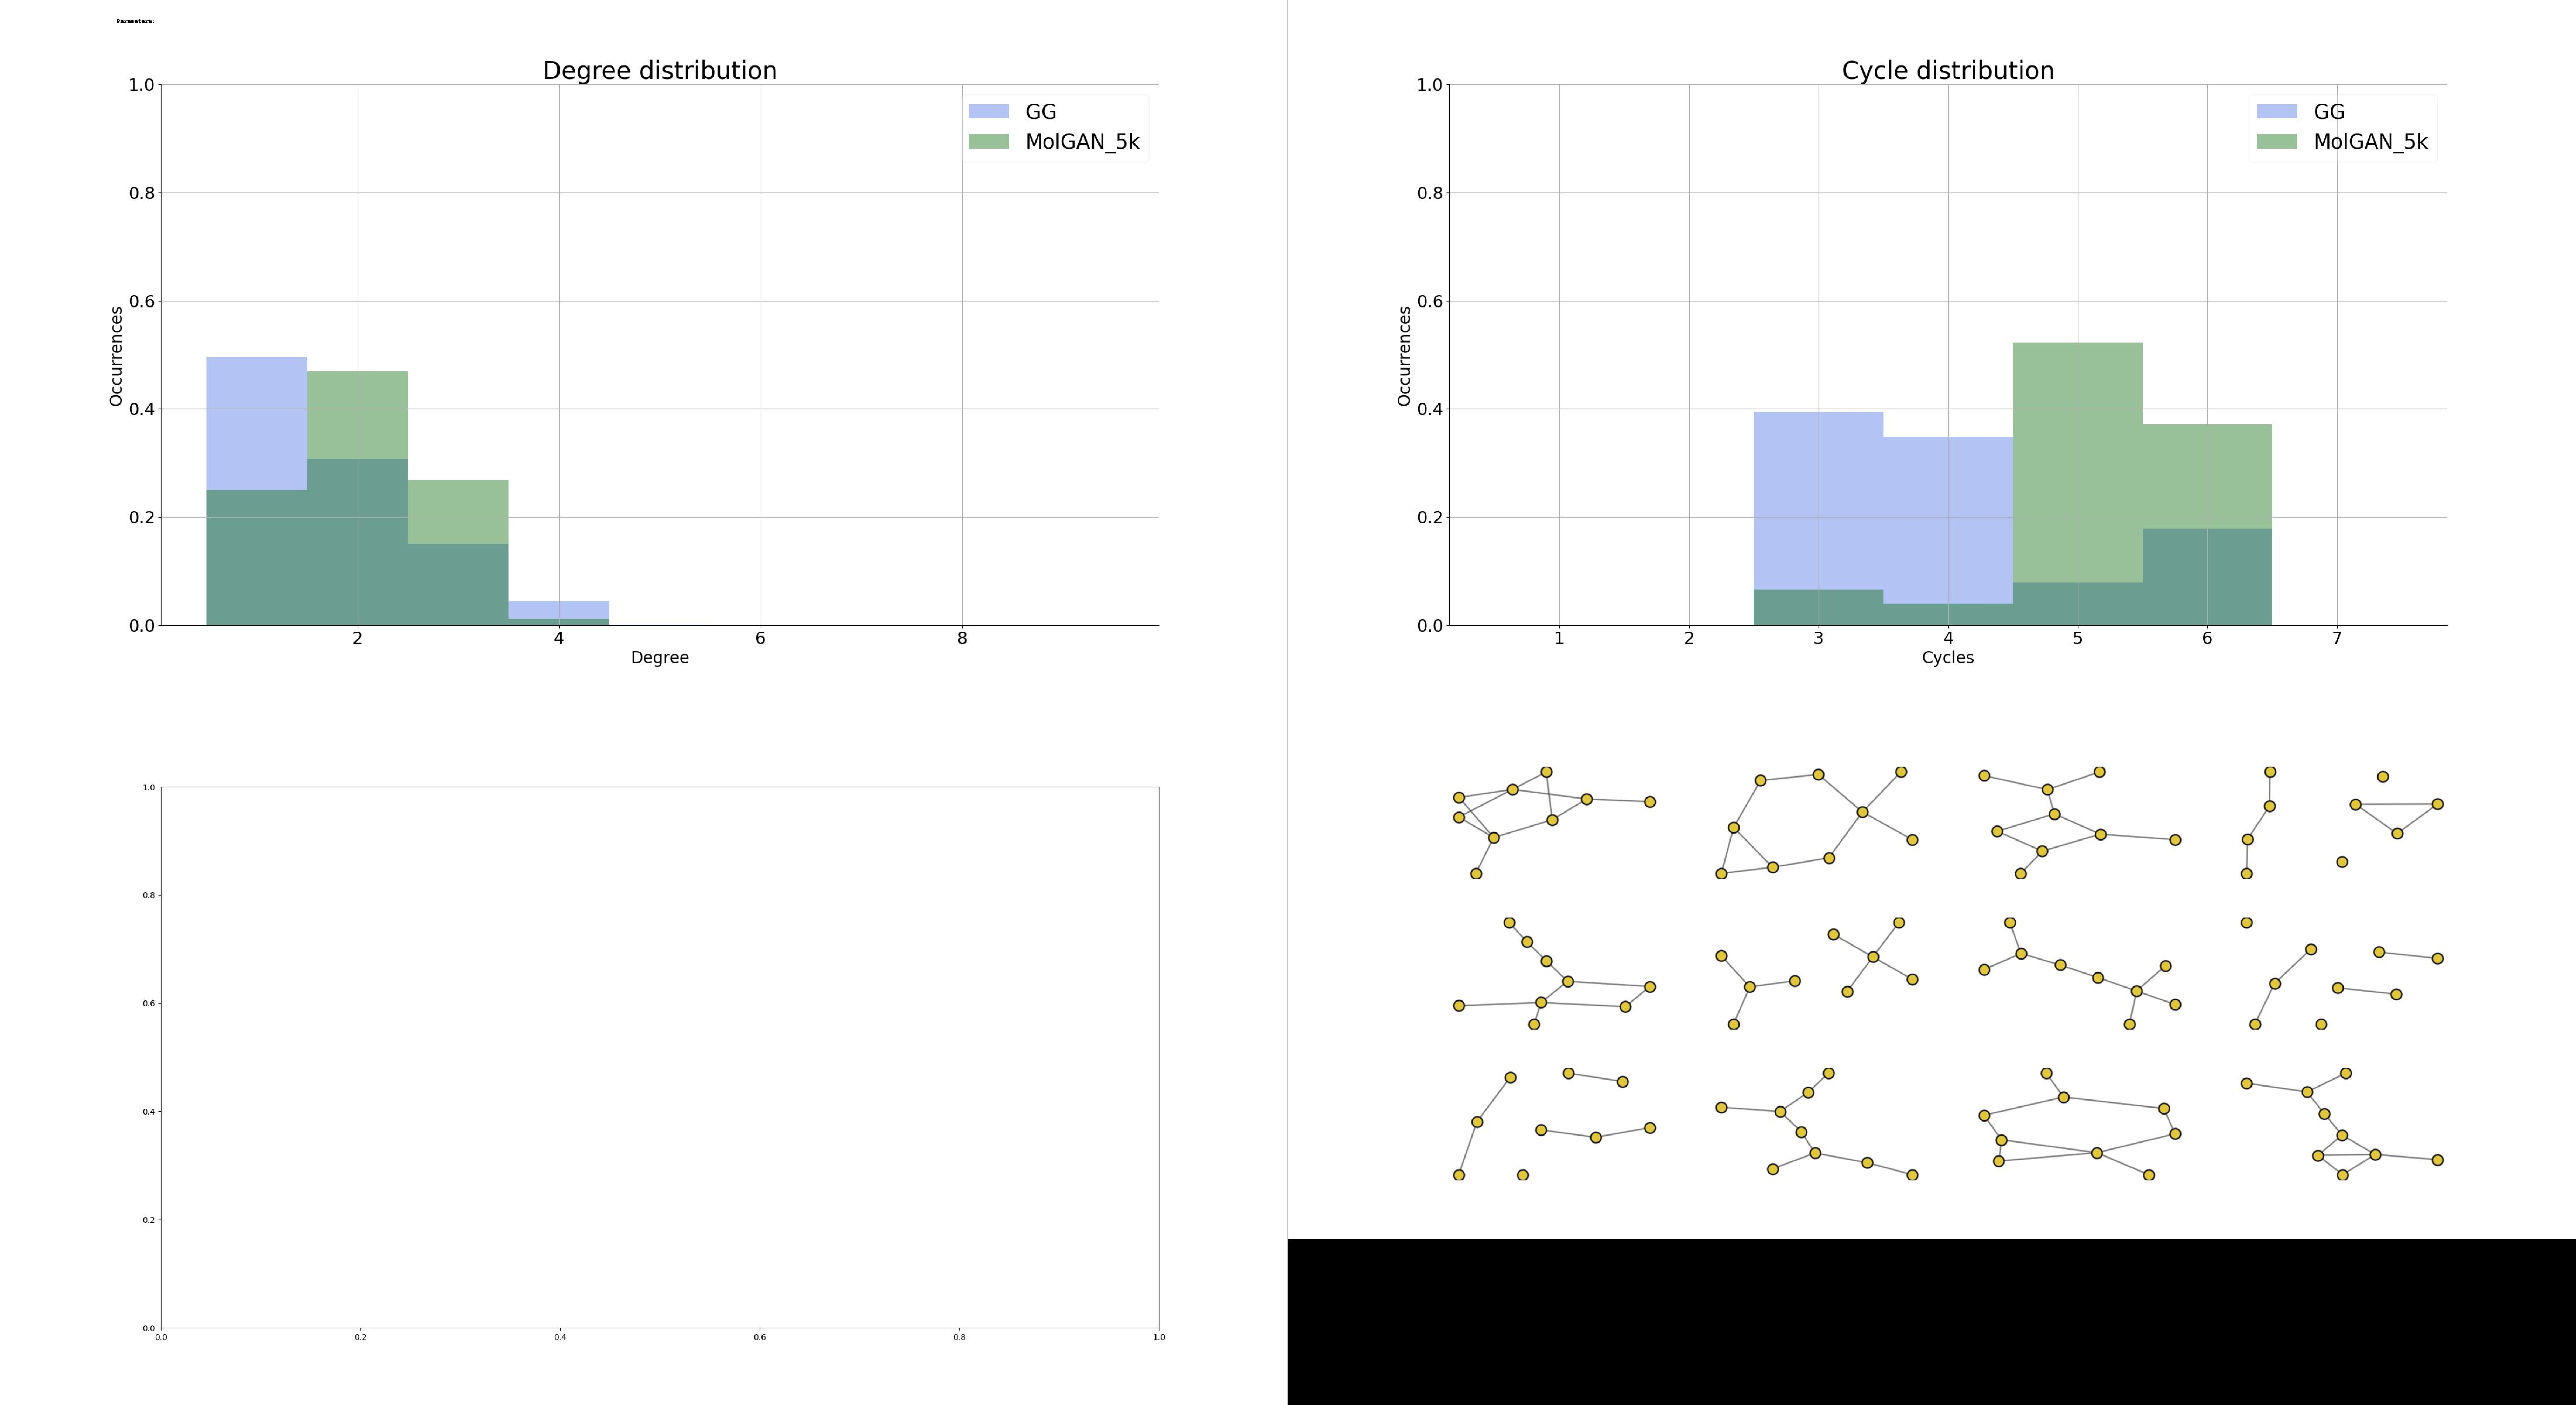
\includegraphics[width=\textwidth]{figures/gggcrp/QM9.pdf}
    \caption{GGG-CRP performance on QM9.}
    \label{fig:qm9}    
    \end{minipage}
    \hfill
    \begin{minipage}{0.475\textwidth}
    \centering
    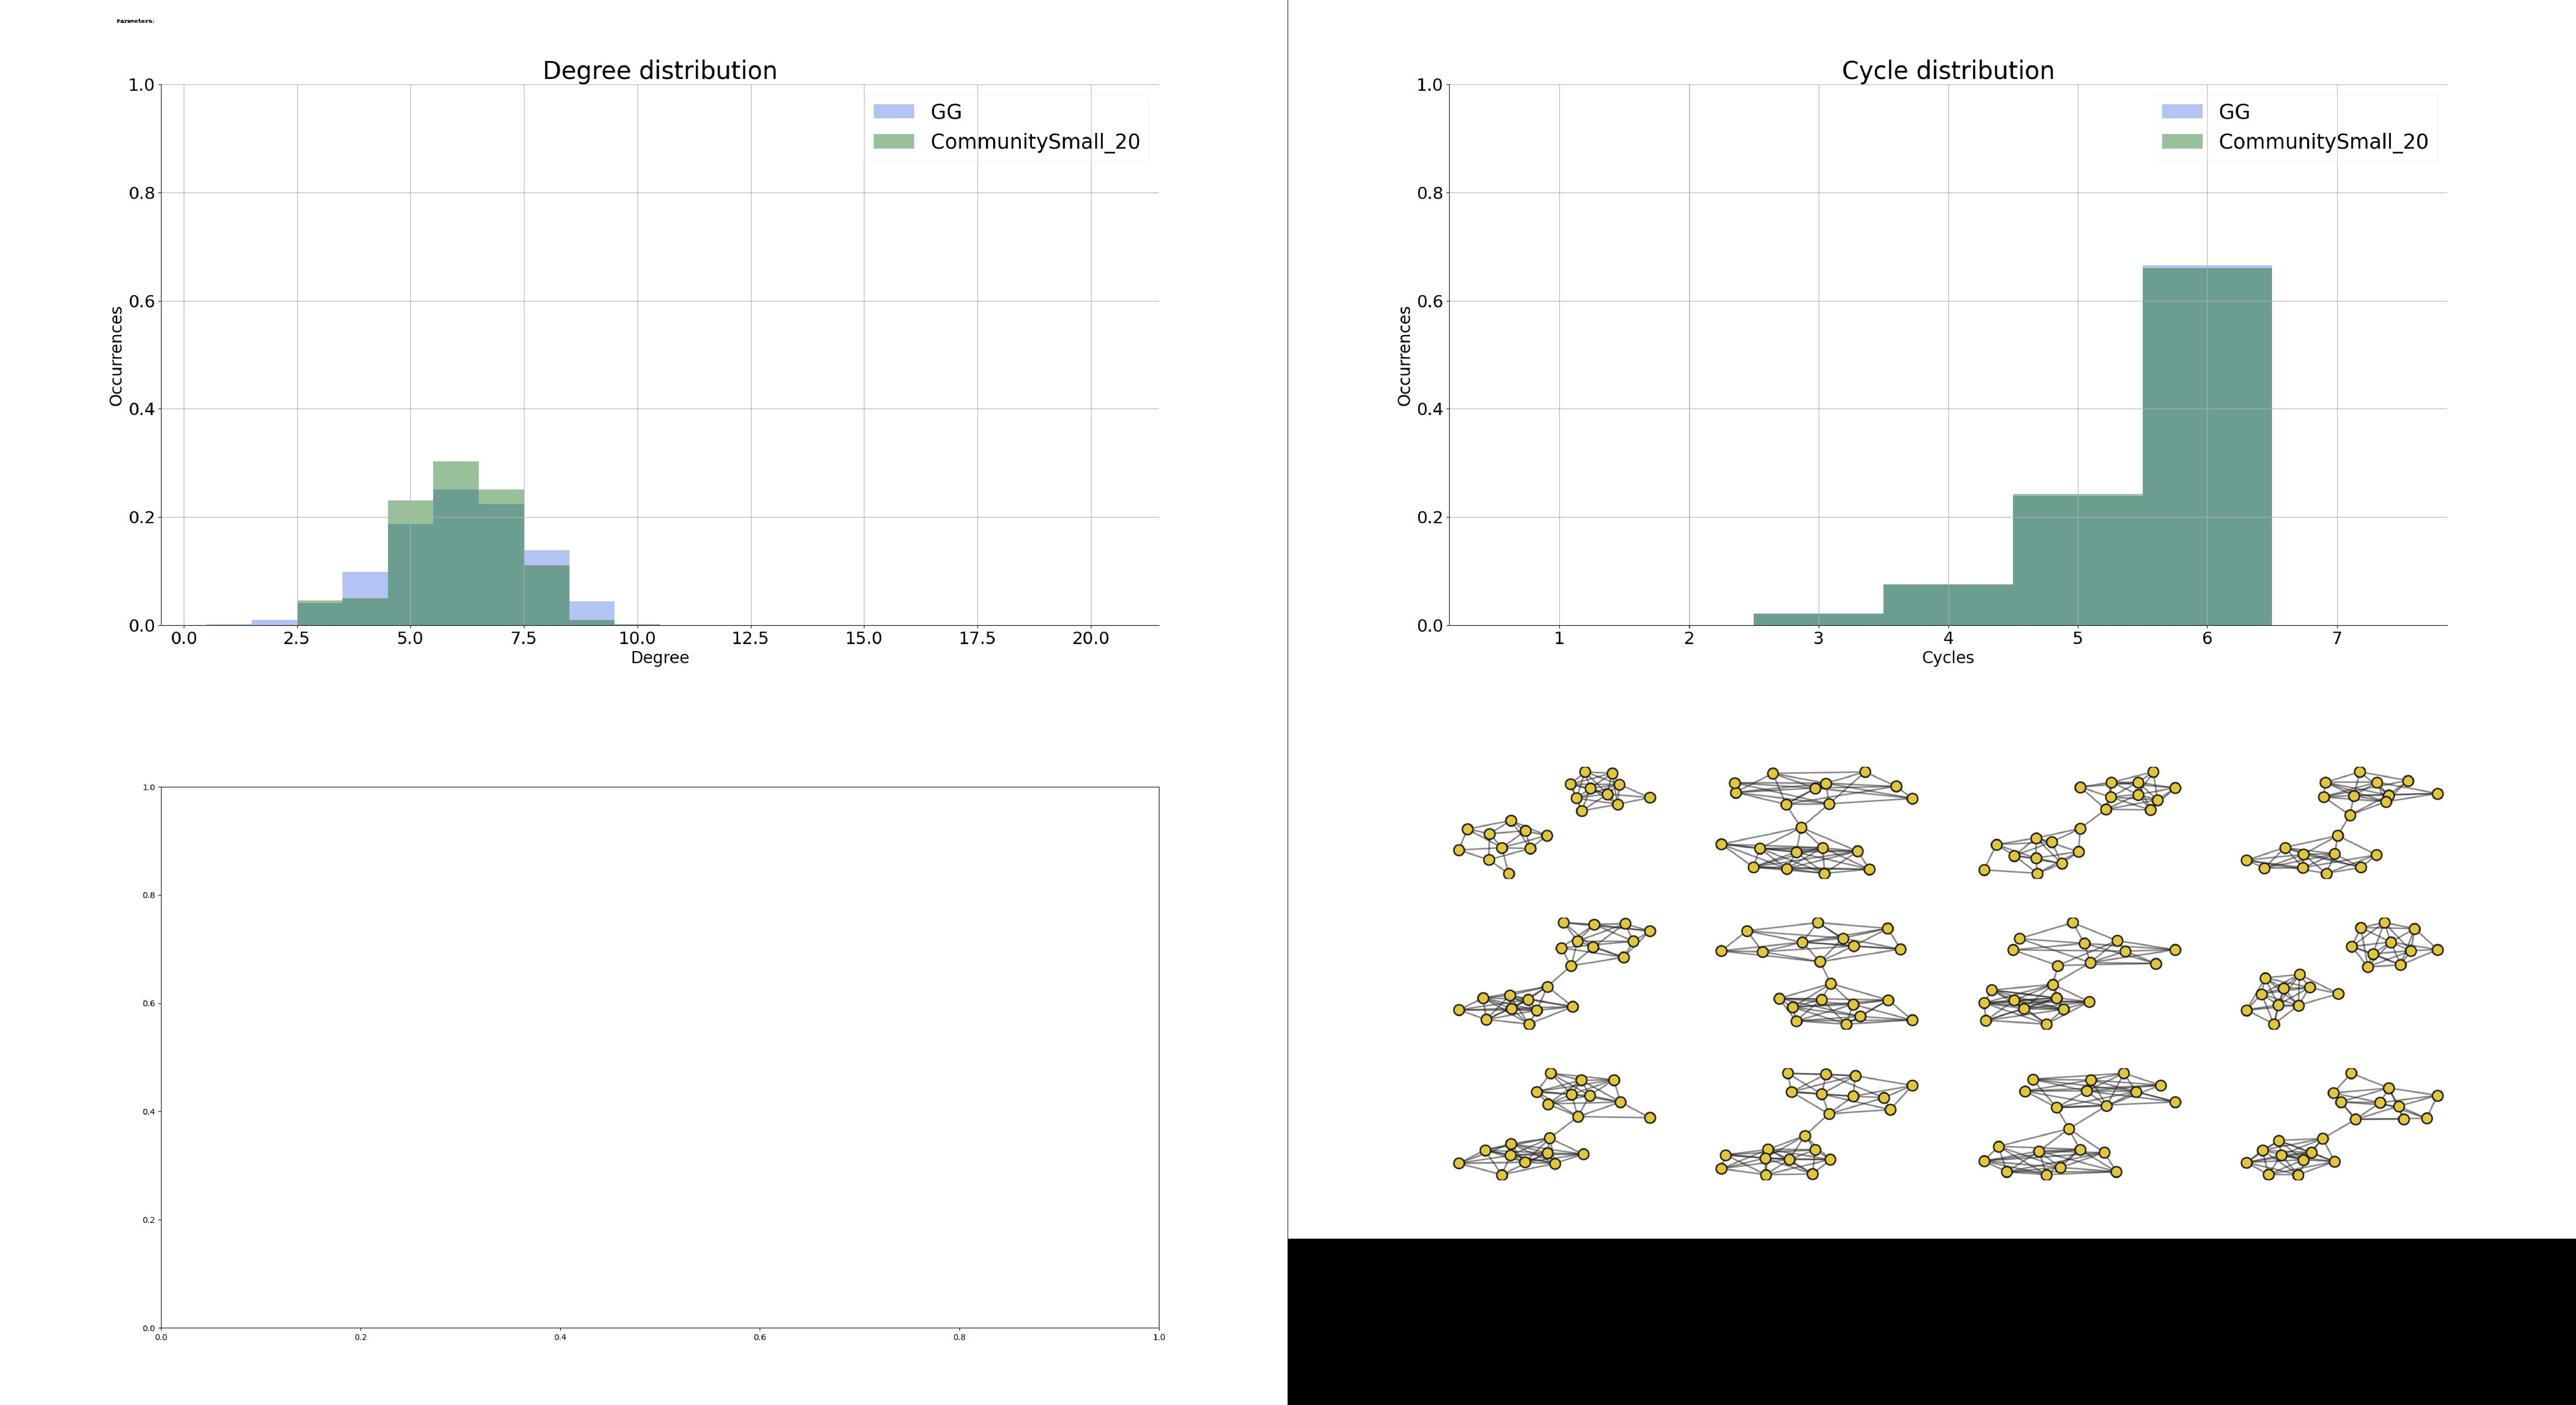
\includegraphics[width=\textwidth]{figures/gggcrp/CommunitySmall_20.pdf}
    \caption{GGG-CRP performance on Community20.}
    \label{fig:community_20}    
    \end{minipage}
    \begin{minipage}{0.475\textwidth}
    \centering
    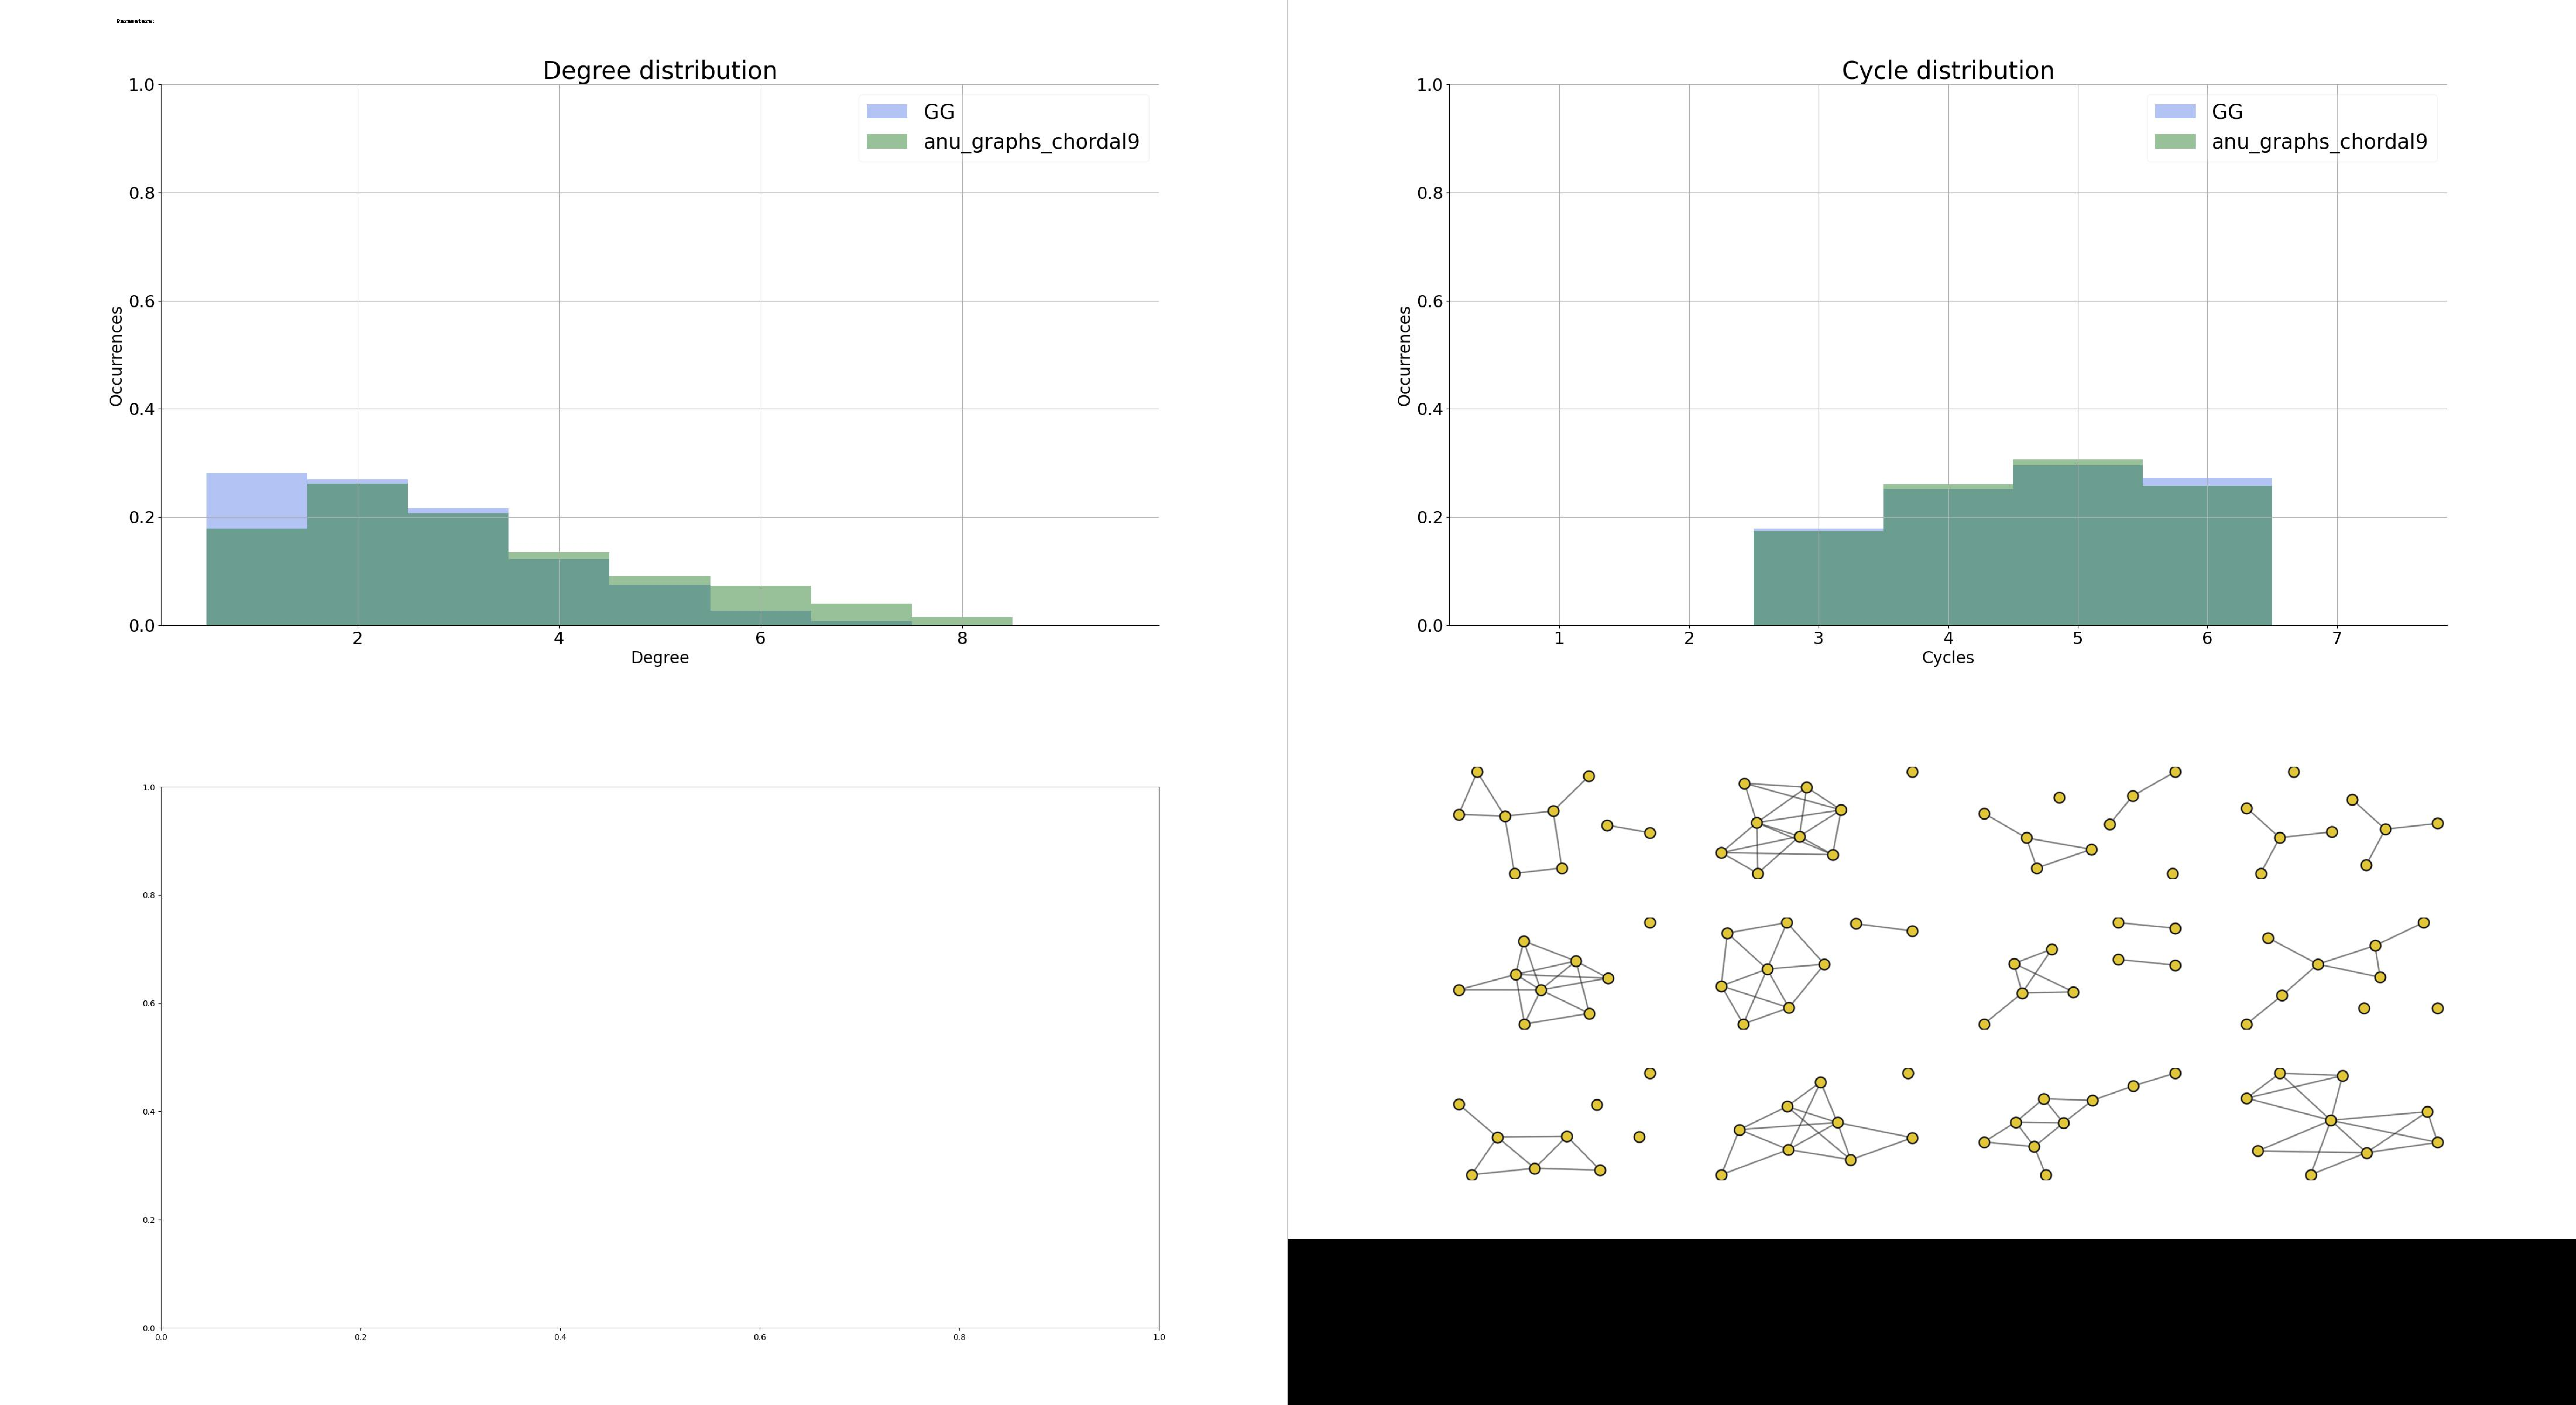
\includegraphics[width=\textwidth]{figures/gggcrp/Chordal9.pdf}
    \caption{GGG-CRP performance on Chordal9.}
    \label{fig:chordal9}    
    \end{minipage}
    \hfill
    \begin{minipage}{0.475\textwidth}
    \centering
    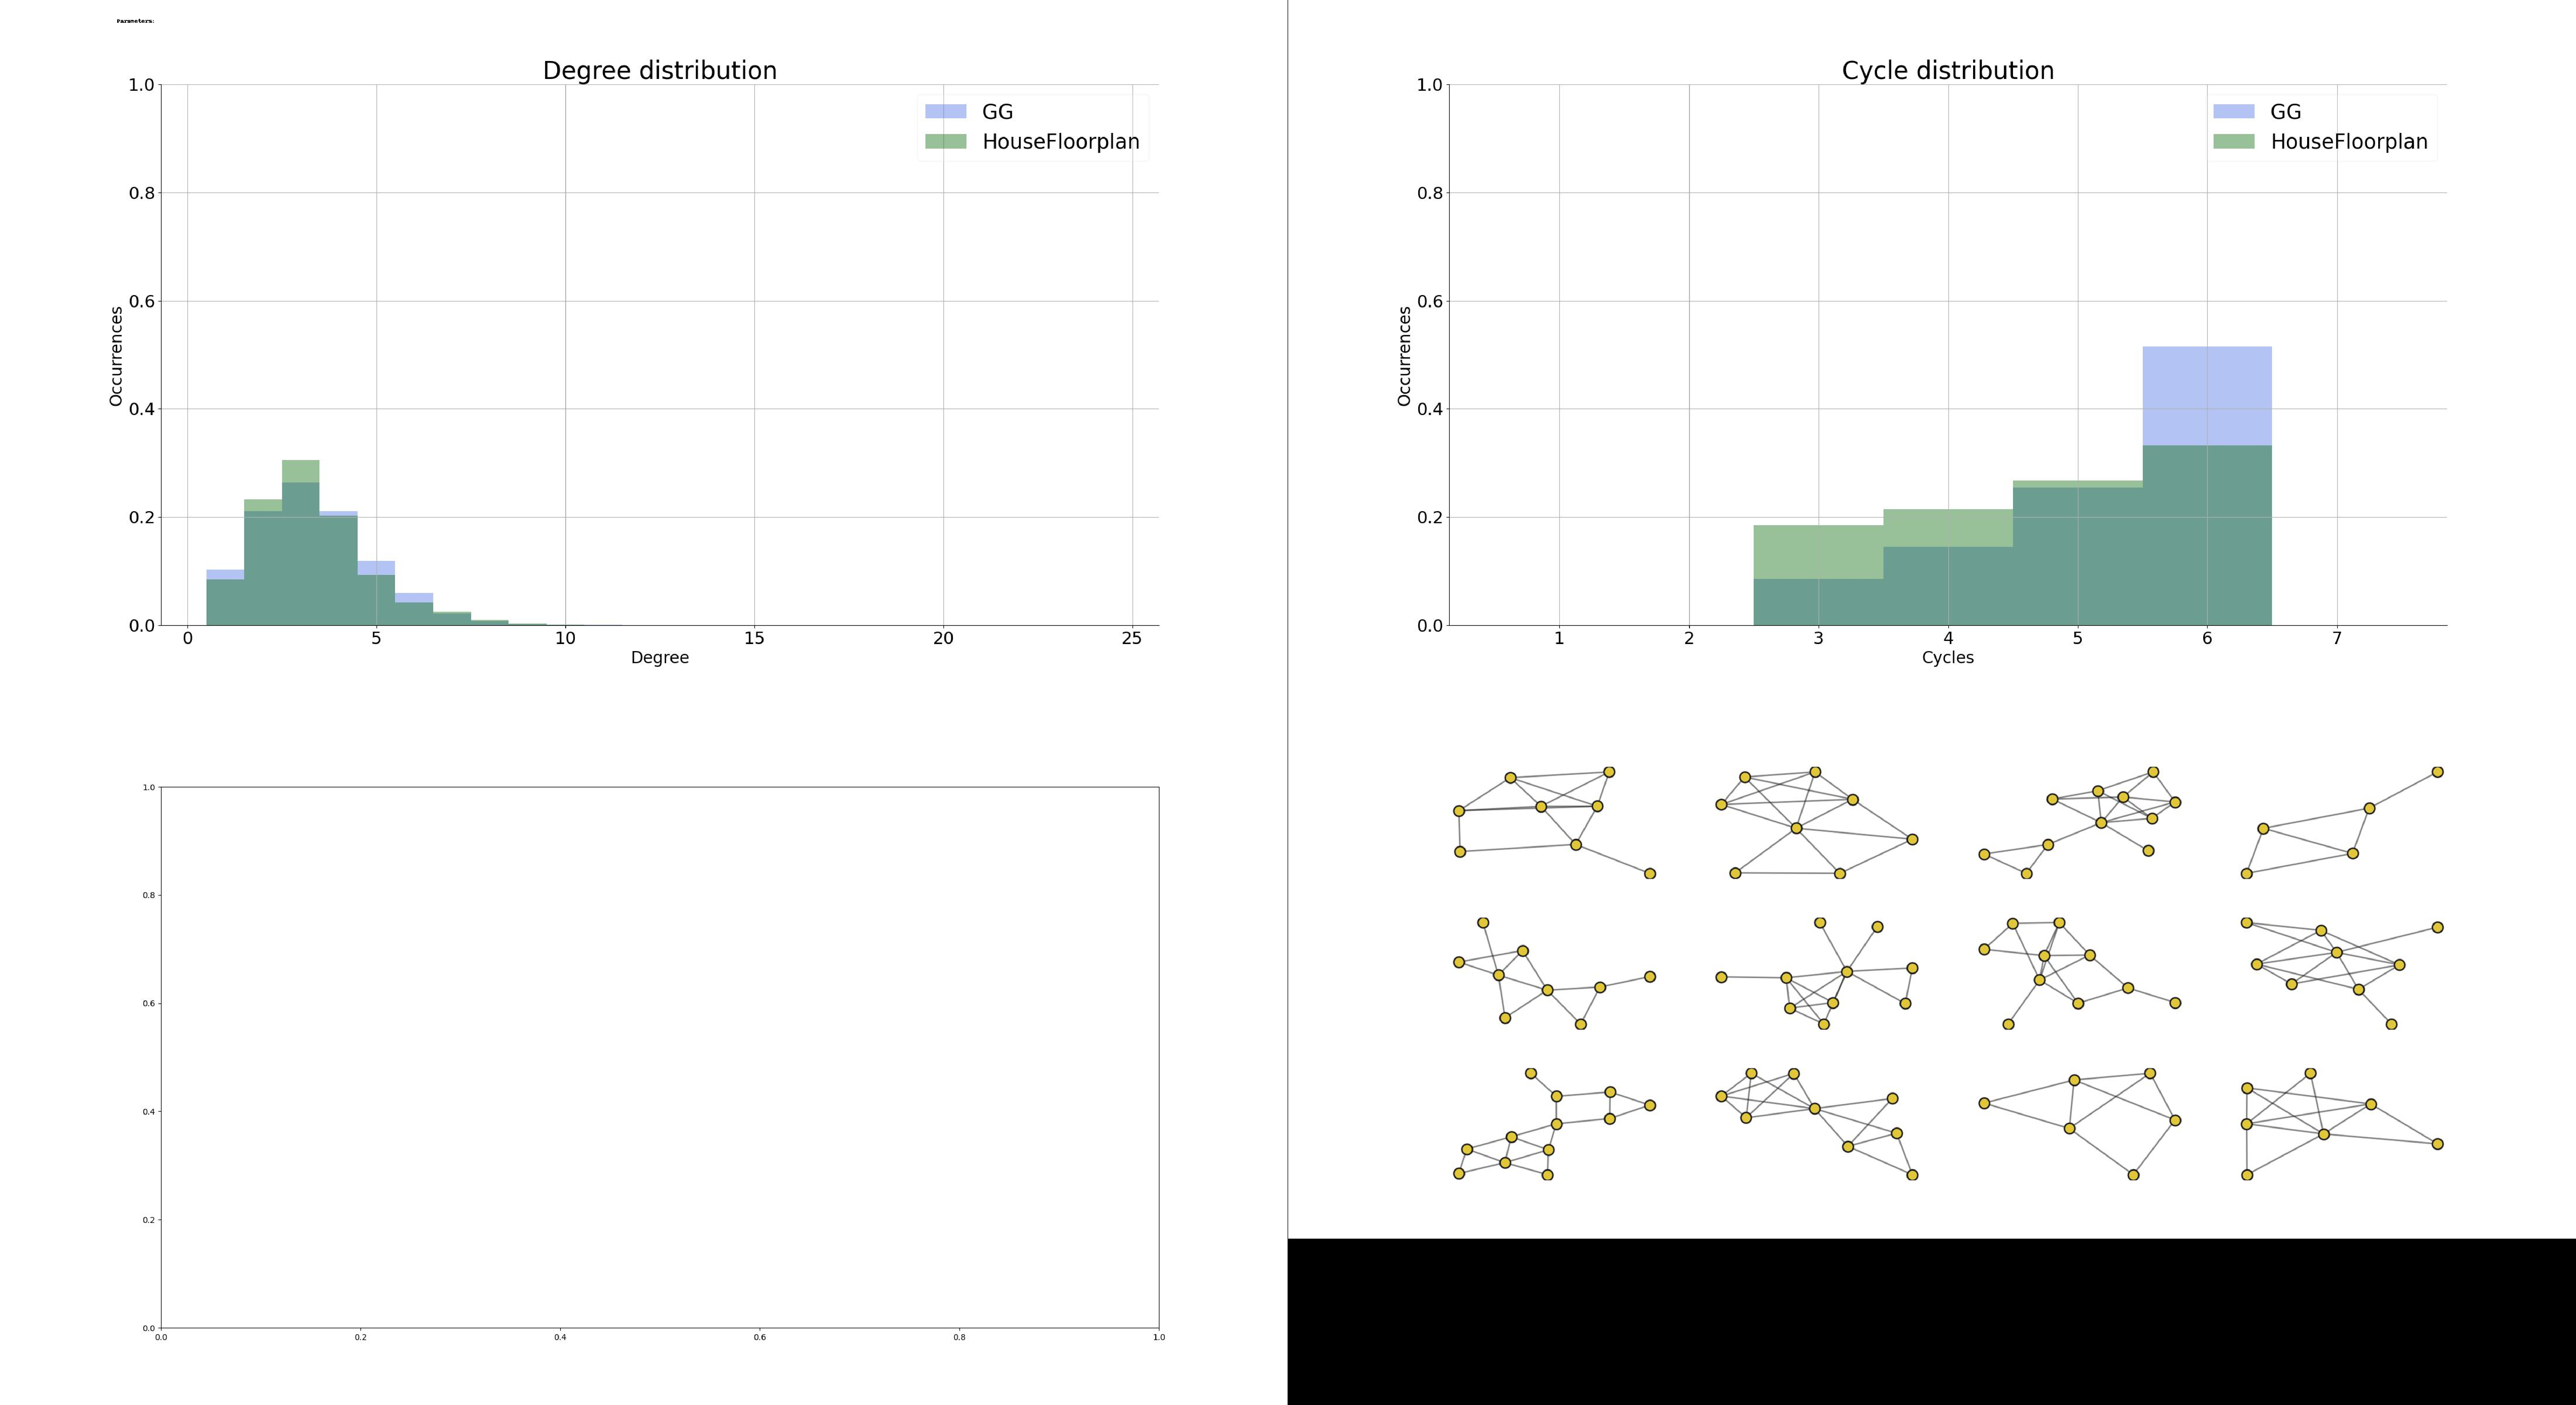
\includegraphics[width=\textwidth]{figures/gggcrp/Housefloorplan.pdf}
    \caption{GGG-CRP performance on HouseFloorplan.}
    \label{fig:house}    
    \end{minipage}
\end{figure}


Table \ref{tab:novelty} presents the number of isomorphism classes generated by each model during evaluation. Unfortunately, even though it seems that the new approach is consistently better, this comparison would only be valid if GGG-CRP had consistently high expressive power as well, since otherwise, less accurate generators naturally produce graphs not present in the dataset. Nevertheless, we are at least satisfied that GGG-CRP does not suffer from a lack of novelty, which is a common issue for other autoregressive models.

\begin{table}[H]
\centering
\caption[Comparison of novelty and diversity between GG-GAN and GGG-CRP.]{Comparison of novelty and diversity between GG-GAN and GGG-CRP. A higher number of isomorphism classes denotes better performance.}
\label{tab:novelty}
% \setlength{\arrayrulewidth}{0.5mm}
%\adjustbox{width=0.475\textwidth}{
\begin{tabular}{lrr}
\toprule
Dataset & GG-GAN & GGG-CRP \\
\midrule
QM9 & 604 & 688 \\
Community20 & 5000 & 5000 \\
Chordal9 & 408 & 2522 \\
HouseFloorplan & / & 3868 \\
\bottomrule
\end{tabular}
%}
\end{table}

We do note another positive behaviour of the GGG-CRP model observed during the training phase: for the Community20 graphs, which possess a very clear community structure, the convergence time compared to the base model was greatly decreased. Less than ten epochs yielded a stable Wasserstein score to obtain the displayed visual results. Autoregressive models in general are known to show greater performance when such graph structures are present, and we are pleased that these benefits are also obtained for our model.

% Due to time constraints, at the time of writing the parameter validation phase for the GG-CRP model unfortunately is in its infancy and the presented results reflect this. However, we believe these initial findings show potential for immediate improvement following extensive testing in future work.

\subsection{Summary}
\label{sec:conclusion}

In this section, we presented an approach on how to integrate permutation-invariant community-detection-based metrics into a Chinese Restaurant Process to perform exchangeable sequence modeling for graph generation. This approach, when integrated into the current best graph GAN model, GG-GAN, yielded a new variation of the model named GGG-CRP. Current results were shown to be comparable to the base model in the wake of strong resource reduction, demonstrating promise. 

\section{Hierarchical Generative Graph Diffusion}
\label{sec: higendiff}

\section{Multi-measurement Methods for Graph Diffusion Acceleration}
\label{sec: multiprox}

In the previous section, we discussed how HiGenDiff can reduce the number of edge probabilities to compute during graph generation and thus reduce time complexity, while preserving very strong generalization performance. However, the choice of employing diffusion models has a negative effect on scalability, as unlike most generative machines, they require $T$ inference steps to produce a sample instead of simple one-shot generation.

This part of the thesis will argue that it is possible to reduce the number of denoising steps required, while also preserving baseline performance. Multi-measurement sampling theory is the key knowledge we must apply to achieve those effects. The content presented in this section is published as \cite{dadi_improving_2025} and is also discussed in \cite{dadi_noisy_2025}.

\subsection{The One True Step}

As we have seen before, denoising diffusion models generate samples by first training a sequence of denoisers at various noise levels and cleverly chaining them to transform unstructured random noise into a sample from a target distribution \cite{ho_denoising_2020, dhariwal_diffusion_2021}. The different noise levels, the methods in which the denoisers are chained, and the balancing of the loss for different noise levels all require careful tuning \cite{karras_elucidating_2022}. So much so that one might ask why we must sample using different noise levels and not simply just one? Why is the annealing (i.e., the gradual decrease of noise) during the sampling stage necessary? 

The reason, as discussed in Section \ref{sec:background_multiprox}, is to break down a difficult sampling problem into a sequence of unimodal sampling problems. Indeed, distributions of interest such as natural images are often multi-modal. The denoising diffusion framework breaks down this sampling task into a sequence of unimodal distributions that are easily approximable by Gaussians. In this work, we show that this sequence of simpler distributions need not be at different noise levels. To propose our framework that operates at a single noise level, we build on ideas from log-concave sampling.

In particular, we build on the work of \cite{saremi_multimeasurement_2021} and earlier investigations in \cite{jain_journey_2022}, which propose a single noise level generative framework. Their sampling process involves sampling from a distribution that is not log-concave. To mitigate this, \cite{saremi_chain_2023} proposes a \emph{chain of log-concave} breakdowns of the task, but at the cost of requiring denoisers at several different noise scales. Moreover, their work merely guarantees that the distributions sampled in their framework are \emph{increasingly} log-concave. The following question remained unanswered
\begin{center}
    \emph{Is there an entirely log-concave single-noise level generative framework?}
\end{center}

In this work, we first study the case when the unnormalized log-density is known to propose the MultiProx sampler. Then, we conduct experiments to show that our framework still yields good results when using a score function from data on real datasets. 


% \begin{figure}
%     \centering
%     \includegraphics[width=0.23\linewidth]{figures/mog_samples.pdf}
%     \includegraphics[width=0.23\linewidth]{figures/mog_samples_second.pdf}
%     \includegraphics[width=0.23\linewidth]{figures/ffhq-small.png}
%     \includegraphics[width=0.23\linewidth]{figures/afhq-small.png}
%     \caption{The MultiProx Sampler on a mixture of Gaussians and on the FFHQ and AFHQ $64\times 64$ datasets. The samples above are generated using \emph{a single MCMC chain}: our sampler is able to traverse in-between modes effectively.}
%     \label{fig:introfig}
% \end{figure}

\subsection{Background}
\label{sec:background_multiprox}

In this preliminary section, we present the necessary background on the variance-preserving variant of Denoising Diffusion Probabilistic Models (DDPMs) \cite{ho_denoising_2020}. Our goal is to characterize the motivation for \emph{time annealing} in diffusion models and question its necessity. 

\subsubsection{DDPMs and the motivation behind annealing}

Recall that, for a data distribution $\mathbf{X}_0 \sim p_0$ over $\mathbb{R}^F$, DDPMs first learn how to denoise by generating noisy versions of $p_0$ (i.e., the forward process). Concretely, noisy measurements $\mathbf{X}_t$, with density denoted $p_t$, of the target distribution are generated as  
\begin{equation}
\mathbf{X}_t = \alpha_t \mathbf{X}_0 +\beta_t Z_t,
\label{eq:noising}
\end{equation}
where $Z_t \sim N\of{\mathbf{0}, \mathbf{I}_F}$ is an independently sampled standard Gaussian; and $\mathbf{X}_0$ is a sample from the data distribution $p_0$. Given these noisy measurements, a network $g_t:\mathbb{R}^F\to\mathbb{R}^F$ is trained to denoise $\mathbf{X}_t$ by learning to predict the noise $Z_t$ given $\mathbf{X}_t$. This boils down to approximating the rescaled score of $\mathbf{X}_t$ given by $-\beta_t \nabla \log p_t$. With simple algebra, we can show that the network is merely a reparametrized approximation to the conditional expectation of $\mathbf{X}_0|\mathbf{X}_t$. In other words, we can show that
\begin{equation}
\label{eq:reparam}
\frac{1}{\alpha_t}\off{X_t - \beta_t g_t\of{\mathbf{X}_t}} = \mathbb{E}\off{\mathbf{X}_0|\mathbf{X}_t}.
\end{equation}
Once the network is trained, diffusion models use this network to progressively denoise a standard Gaussian to generate new samples. The network has learned to compute conditional expectations, and the goal of the denoising process is to exploit these conditional expectations to output a new sample. If $T$ is the largest amount of noise added during training, the denoising process starts from an approximation $\tilde{\mathbf{X}}_T$ of $\mathbf{X}_T$, which is sampled from a standard Gaussian $N\of{\mathbf{0}, \mathbf{I}_F}$. The closer the distribution of $\tilde{\mathbf{X}}_T$ is to $p_T$, the better: the quality of the Gaussian initialization improves as $T$ increases since the larger $T$ is, the closer $p_T$ is to $N\of{\mathbf{0}, \mathbf{I}_F}$. After the initialization, the denoising is achieved by simulating the reverse process. A single step of the latter yields the following Gaussian approximation, 
\begin{equation}
\label{eq:revdiff}
    \mathbf{X}_0|\mathbf{X}_T \approx \mathbb{E}\off{\mathbf{X}_0|\mathbf{X}_T} + \sigma_T Z,
\end{equation}
where $Z \sim N\of{\mathbf{0}, \mathbf{I}_F}$. Unfortunately, this single-step estimation of $\mathbf{X}_0$ from $\mathbf{X}_T$ becomes increasingly poor as $T$ becomes large. This large discrepancy between $\mathbf{X}_0|\mathbf{X}_T$ and its Gaussian approximation $N\of{\mathbb{E}\off{\mathbf{X}_0|\mathbf{X}_T}, \sigma_T \mathbf{I}_F}$ is the \emph{central motivation for time-annealing}. One-step denoising does not work because $\mathbf{X}_0|\mathbf{X}_T$ is too multi-modal. Indeed, \emph{multi-modal distributions are not well approximated by their expectation}, so we must progressively denoise in smaller steps where multi-modality is not an issue and each individual step is well-approximated by a Gaussian distribution. 

To restate the trade-off: the one-step Gaussian approximation is increasingly worsened by large choices of $T$, yet we must choose $T$ to be large in order for the initialization at $\hat{\mathbf{X}}_T$ to be valid. Time annealing is precisely the design choice that allows diffusion models to balance these competing trade-offs. For any large $T$, we can define a discretization sequence $0 = t_0 < t_1 < \dots < t_N = T$ such that the Gaussian approximation $
\mathbf{X}_{t_{i-1}}|\mathbf{X}_{t_{i}} \approx \mathbb{E}\off{\mathbf{X}_{t_{i-1}}|\mathbf{X}_{t_{i}}} + \sigma_{t_{i-1}} Z_{t_{i-1}},$
where $Z_{t_{i-1}} \sim N\of{\mathbf{0}, \mathbf{I}_F}$ is valid. These Gaussian approximations using the conditional expectation correspond precisely to the exponential integration scheme with $N$ discretization points applied to \ref{eq:revdiff}. This is the reason why annealing is necessary: it breaks down the difficult multi-modal sampling step of going from $\mathbf{X}_T$ to $\mathbf{X}_0$ into a sequence of uni-modal sampling problems $\mathbf{X}_{t_{i-1}}|\mathbf{X}_{t_i}$. 

Diffusion models are a sequence of Gaussian approximations, and time annealing is what makes these Gaussian approximations valid by defining a sequence of steps over which Gaussian approximations using the learned conditional expectations are appropriate. This comes at a cost: a series of conditional expectations $\mathbb{E}\off{\mathbf{X}_{t_{i-1}}|\mathbf{X}_{t_{i}}}$ must be approximated, which requires denoisers at different noise scales.

\subsubsection{The disadvantages of time annealing}

Having expounded on the motivation for time-annealing, we now argue that time-annealing comes with critical drawbacks.

First, annealing is taxing to the denoising network. In practice, the most successful denoising networks are built on the ADM networks of \cite{dhariwal_diffusion_2021}, which have been carefully improved in \cite{karras_analyzing_2024}. There, a single network is trained to denoise samples at varying noise scales, where a separate component informs the network of the noise level.

The task of denoising varies greatly at different noise scales. At high-noise levels, the denoiser must learn how to introduce low-frequency elements in the samples; at low-noise levels, it must act solely on the high frequencies to introduce detail. Performing both these tasks using the same network requires careful balancing of the training loss. Indeed, as observed in \cite{karras_analyzing_2024}, a multi-task training approach is adopted to stabilize training. Denoising different noise levels can be so radically different that recent work \cite{balaji_ediff-i_2022} trains an ensemble of denoisers that separately focus on the high-noise and low-noise stages. In addition to the architectural difficulties, time annealing also introduces tuning difficulties: the training noise schedule was observed to be highly sensitive to the output resolution in \cite{chen_importance_2023}. Finally, taking inspiration from \cite{rissanen_generative_2022, dieleman_diffusion_2024}, we perform a frequency analysis on intermediate images generated during the denoising process of a standard diffusion model, EDM \cite{karras_elucidating_2022}.
 % Figure \ref{fig:wastednoise} illustrates the power spectrum throughout the denoising stages of EDM, which was trained on the FFHQ dataset. 
 We observed that the time-annealing schedule, despite requiring architectural modifications and meticulous tuning, results in a significant portion of the denoising process adding minimal structural detail to the samples. %Specifically, the bottom middle plot of Figure \ref{fig:wastednoise} demonstrates that 
 The spectrum remains flat, akin to white noise, for a substantial part of the process.

In summary, while time annealing is a pivotal component as discussed earlier in this section, it places a considerable demand on the design of denoising architectures and necessitates precise tuning that is both resolution and dataset-dependent. Yet, a significant part of this process is spent without contributing any meaningful structure to the samples. 

In the ensuing sections, we will introduce an alternative approach to decomposing the sampling task. This method does not require a time-embedding sub-network and alleviates the tuning burden by reducing the number of variables involved, offering a more streamlined and efficient framework.

% \begin{figure}[t]
%     \centering
%     \includegraphics[width=0.7\linewidth]{figures/rapsB.pdf}
%     \caption{A visualization of the average spectral power density throughout the denoising process of EDM \cite{karras2022elucidating} on FFHQ64: Observe that pure noise has a flat power spectrum (bottom left) and natural images have a linearly decreasing power spectrum on a log-log plot (bottom right) since lower frequencies dominate in natural images. We plot the power spectrum of the intermediate images in the denoising process (middle). Observe that the first half of the denoising acts on all frequencies by lowering the power spectrum \emph{but does not add structure}, it is only later in the process that the denoising starts acting on higher frequencies and adds structure in the images.}
%     \label{fig:wastednoise}
% \end{figure}

\subsection{Related work}

\paragraph{Diffusion Monte Carlo} Our work builds on previous schemes that mix ideas from log-concave sampling and denoising diffusions.
\cite{huang_reverse_2023} first introduces the idea of inner Langevin loops for sampling from potentials and provides a theoretical analysis. Similar ideas also appear in \cite{mcdonald_proposal_2022} and \cite{vargas_denoising_2023}, which incorporate score estimation for diffusive sampling, as do \cite{akhound-sadegh_iterated_2024}. \cite{chen_diffusive_2024} proposes DiGs, which corresponds exactly to the proximal sampler of \cite{shen_composite_2020} made practical with MALA as an approximation. They circumvent the difficulty of sampling from high-noise levels by initializing in a \enquote{clever way}, which, unlike our proposal, is only a heuristic. \cite{he_zeroth-order_2024} suggests a zeroth-order method to improve over the proximal sampler. \cite{phillips_particle_2024} also proposes a sequential Monte Carlo scheme based on diffusions. The work of \cite{chehab_practical_2024} reviews all recent tempering schemes. Crucially, the fundamental difficulty of the \emph{duality of log-concavity} which underlies sampling tasks is detailed in \cite{grenioux_stochastic_2024}. It is this difficulty that our scheme addresses.

% \paragraph{The Restricted Gaussian Oracle (RGO) in the literature:} Practical implementations of the RGO of \cite{shen2020composite} appears in earlier forms in \cite{gao2020learning} and \cite{xiao2021tackling}.

\paragraph{Multi-measurement process} Using multiple correlated measurements appears in \cite{saremi_multimeasurement_2021} and \cite{saremi_chain_2023}. More generally, multi-measurements correspond to linear observation as defined in \cite{montanari_posterior_2023} or posterior sampling in linear regression with fixed design.

\subsection{The MultiProx samplers}
In section \ref{sec:appendix_gibbs} of the appendix, we theoretically show how Gibbs multimeasurement is an entirely log-concave sampling framework. Each individual sampling step is also computationally tractable, and each sampling step in Algorithm \ref{alg:pipeline} can be implemented exactly. We derive from this result an implementation of our framework we call the MultiProx sampler, as Algorithm \ref{alg:multiprox}.

\begin{algorithm}[H]
    \caption{The MultiProx sampler}
    \label{alg:multiprox}
    \begin{algorithmic}
        \STATE{\textbf{input} number of stages $n$, Gibbs ensemble size $m$, sampling frequency $p<m$, fixed noise level $t<T$, diffusion model generators $\offf{g_u}_{u=1}^{T}$}
        \STATE{$\hat{\mathbf{Y}}_1, \dots, \hat{\mathbf{Y}}_m \sim N\of{\mathbf{0},\mathbf{I}_{m F}}$}
        \FOR{$i \gets 1$ to $n$}
        \FOR{$j \gets 1$ to $m$}
        \STATE{$\hat{\mathbf{X}}_j\gets\frac{1}{m}\sum_{k=1}^{m}{\hat{\mathbf{Y}}_k}$}
        \STATE{$\hat{\mathbf{X}}_j \gets g_t\of{\hat{\mathbf{X}}_j}$}
        \IF{$p \mid j$}
        \STATE{\textbf{yield} $\hat{\mathbf{X}}_j$}
        \ENDIF
        \STATE{$\hat{\mathbf{Y}}_j \gets \hat{\mathbf{X}}_j$}
        \ENDFOR
        \ENDFOR
    \end{algorithmic}
\end{algorithm}

Figure \ref{fig:multiprox} summarizes the MultiProx algorithm and its theoretical properties. Namely, note how with specific conditions on the number of multimeasurements $m$ and the fixed noise level $t$, Gibbs sampling provides us with a fully log-concave single-noise level denoising diffusion sampling framework. While the Gibbs sampling itself can easily be implemented with simple averaging and replacement of each multimeasurement one by one.

\begin{figure}[H]
    \centering
    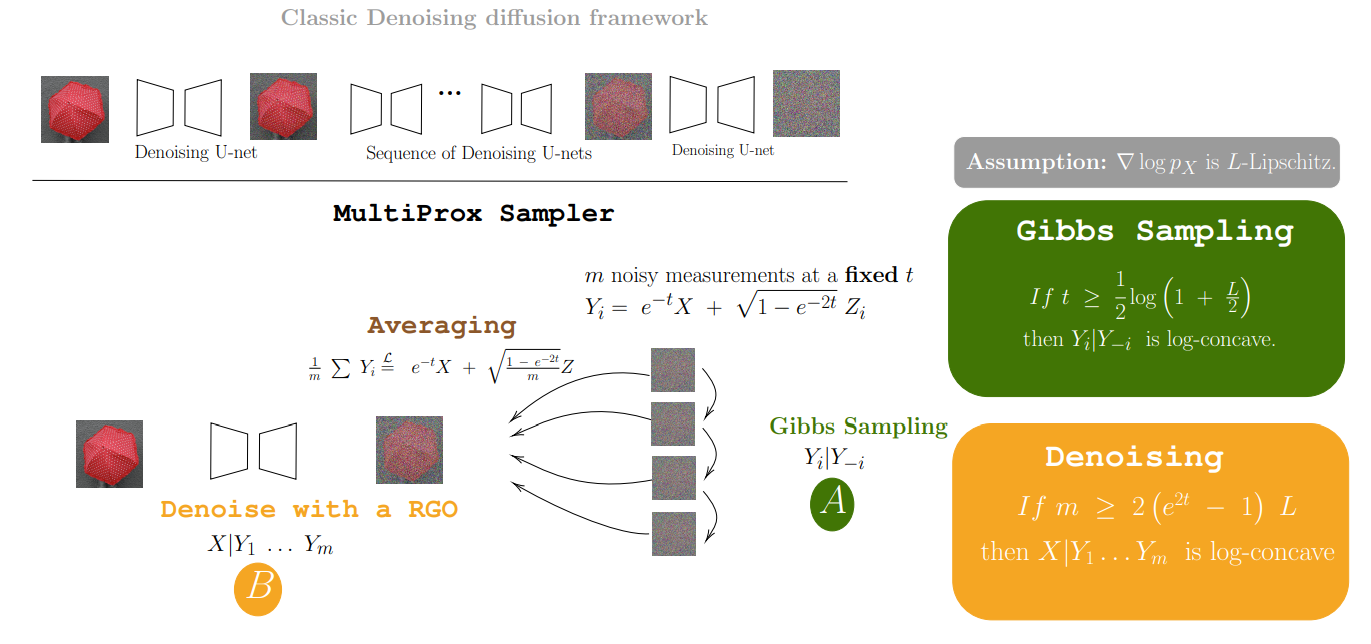
\includegraphics[width=\textwidth]{figures/multiprox/diagram.png}
    \caption[MultiProx diagram.]{Diagram of the operation of the MultiProx algorithm and the associated theoretical results, in comparison to the annealing baseline.}
    \label{fig:multiprox}
\end{figure}

Nevertheless, we did question the possibility that the assumption of Gaussian latent noise being appropriate for all non-modal distributions is invalid. In such a case, we hypothesize that sampling from a single noise level could be insufficient. We thus also consider allowing a few annealing steps to a second lower noise level $t' \leq t$ before outputting a sample and using it for Gibbs sampling. We refer to this modified sampling algorithm as MultiProxAn, whose pseudocode is given in Algorithm \ref{alg:multiproxan}.

\begin{algorithm}[H]
    \caption{The MultiProxAn sampler}
    \label{alg:multiproxan}
    \begin{algorithmic}
        \STATE{\textbf{input} number of stages $n$, Gibbs ensemble size $m$, sampling frequency $p<m$, fixed noise levels $t' \leq t<T$, diffusion model generators $\offf{g_u}_{u=1}^{T}$}
        \STATE{$\hat{\mathbf{Y}}_1, \dots, \hat{\mathbf{Y}}_m \sim N\of{\mathbf{0},\mathbf{I}_{m F}}$}
        \FOR{$i \gets 1$ to $n$}
        \FOR{$j \gets 1$ to $m$}
        \STATE{$\hat{\mathbf{X}}_j\gets\frac{1}{m}\sum_{k=1}^{m}{\hat{\mathbf{Y}}_k}$}
        \STATE{$\hat{\mathbf{X}}_j \gets \textcolor{blue}{\of{g_{t} \circ \dots \circ g_{t'}}}\of{\hat{\mathbf{X}}_j}$}
        \IF{$p \mid j$}
        \STATE{\textbf{yield} $\hat{\mathbf{X}}_j$}
        \ENDIF
        \STATE{$\hat{\mathbf{Y}}_j \gets \hat{\mathbf{X}}_j$}
        \ENDFOR
        \ENDFOR
    \end{algorithmic}
\end{algorithm}

\subsection{Experiments}

In this section, we present the results of a series of experiments conducted with MultiProx to confirm its effectiveness at sampling from multimodal distributions.

For most cases of interest, the log-density is not available and needs to be learnt from samples. In this case, exact Gibbs sampling techniques become too expensive to execute. For this reason alone, in the MultiProx pseudocode and in implementation, we approximate the true Restricted Gaussian Oracle (RGO) with the generator networks. Importantly, note that we do not retrain the diffusion models; we simply replace the annealing sampling strategy employed during evaluation with our own.

% \begin{figure}
%     \centering
%     \includegraphics[width=0.4\linewidth]{figures/GMM.pdf}
%     \caption{Visualization of 1000 samples from a single chain on a mixture of 40 Gaussians.}
%     \label{fig:gmm}
% \end{figure}

% \subsubsection{Mixture of 40 Gaussians}

% To begin, we consider a classic synthetic problem of a mixture of Gaussians with 40 components (see Figure \ref{fig:gmm}). We run our sampler with parameters $m = 4$ and $\sigma = 150 \sqrt{m}$. For the RGO, we need to find the optimum $x_y^\star$ defined in \ref{alg:rgo}. We use the BFGS optimizer with a maximum of 256 steps implemented in the optimistix package \footnote{https://github.com/patrick-kidger/optimistix}. We also measure the Wassertein distance between 1000 generated samples and 1000 ground truth samples and report the metrics in Table \ref{tab:perf_comparison_simple} under GMM-40. Our samples are generated from a single  1500 step chain, the first 500 steps being warm-up steps.

%\subsection{Multi-particle energy functions}

%We evaluate MultiProx on two energy functions for multi-particle systems. The Double-Well Potential (DW-4) computes the energy of 4 $2D$-particles. The sampling problem is thus an $ 8$-dimensional problem outputting the positions of the particles. Since the energy is rotation, translation and permutation invariant, we measure the pair-wise distance Wassertein metric, which measures the Wassertein distance between the distributions of pair-wise distances between the particles generated by MultiProx and the ground truth provided by \cite{akhound2024iterated}. The Lennard-Jones potential LJ-13 is a 13-particle system in $3D$. The problem is of dimension $39$. 

\subsubsection{Learnt score functions for images}
% \begin{table} % Float placement: here, top, bottom, page

% \centering % Center the table on the page

% \caption{Performance comparison of different methods on GMM-40. Values are reported as mean $\mathcal{W}_2$ distance $\pm$ standard deviation over 3 runs. Lower values indicate better performance.}

% \label{tab:perf_comparison_simple} % A descriptive label for cross-referencing

% \begin{tabular}{lc} % l: left-align (Method), c: center-align (numerical columns)

% \toprule

% Method          & GMM-40(d = 2)        \\

% \midrule

% FAB \cite{midgley2022flow}             & $12.0 \pm 5.73$            \\ % {---} produces an em-dash, good for N/A

% PIS \cite{zhang2021path}         & $7.65 \pm 0.92$ \\

% DDS \cite{vargas2023denoising}             & $9.32 \pm 0.82$ \\

% iDEM \cite{akhound2024iterated}           & $7.42 \pm 3.44$ \\

% \textbf{MultiProx}(Ours) & \textbf{$\mathbf{6.51 \pm 0.36}$}  \\

% \bottomrule

% \end{tabular}

% \end{table}
Figure \ref{fig:multiprox_images} displays Gibbs chains of samples from 3 image datasets: CIFAR10 \cite{krizhevsky_learning_2009}, AFHQ \cite{choi_stargan_2020} and FFHQ 64x64 \cite{karras_style-based_2019}. We observe how, after a few \enquote{warm-up} iterations, the chains smoothly interpolate between the complicated image modes.

\begin{figure}[H]
    \centering
    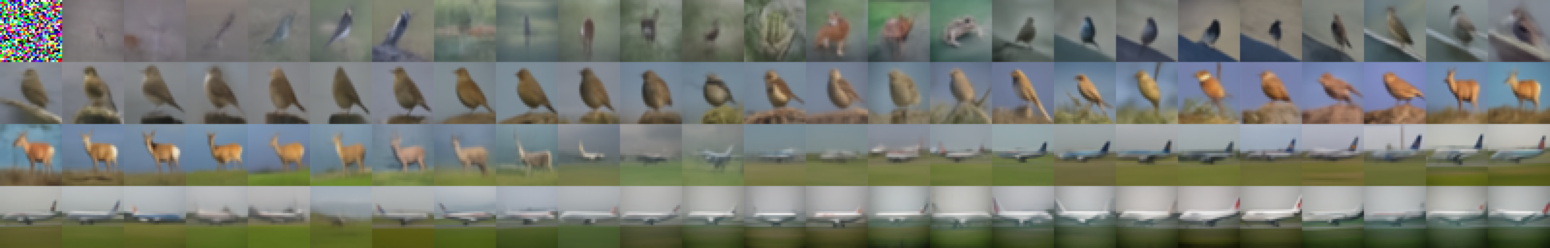
\includegraphics[width=0.49\linewidth]{figures/multiprox/cifar10.png}
    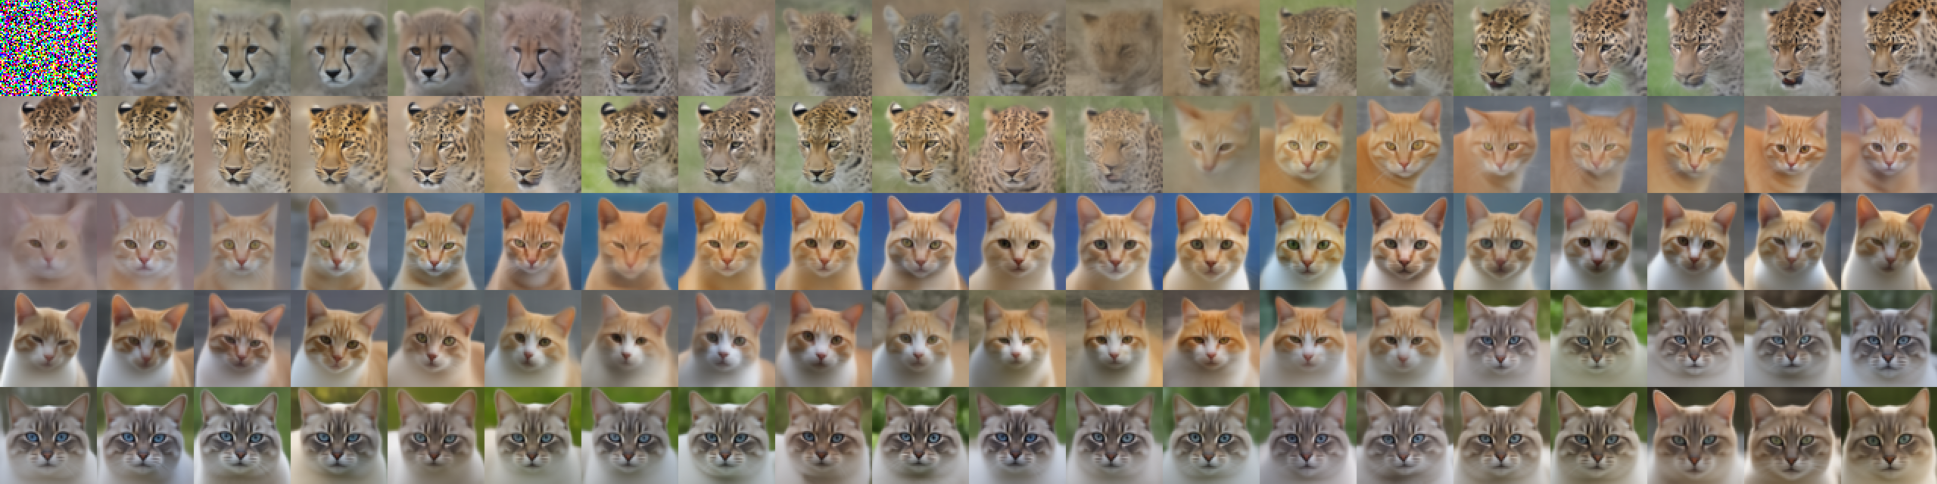
\includegraphics[width=0.49\linewidth]{figures/multiprox/afhq.png}
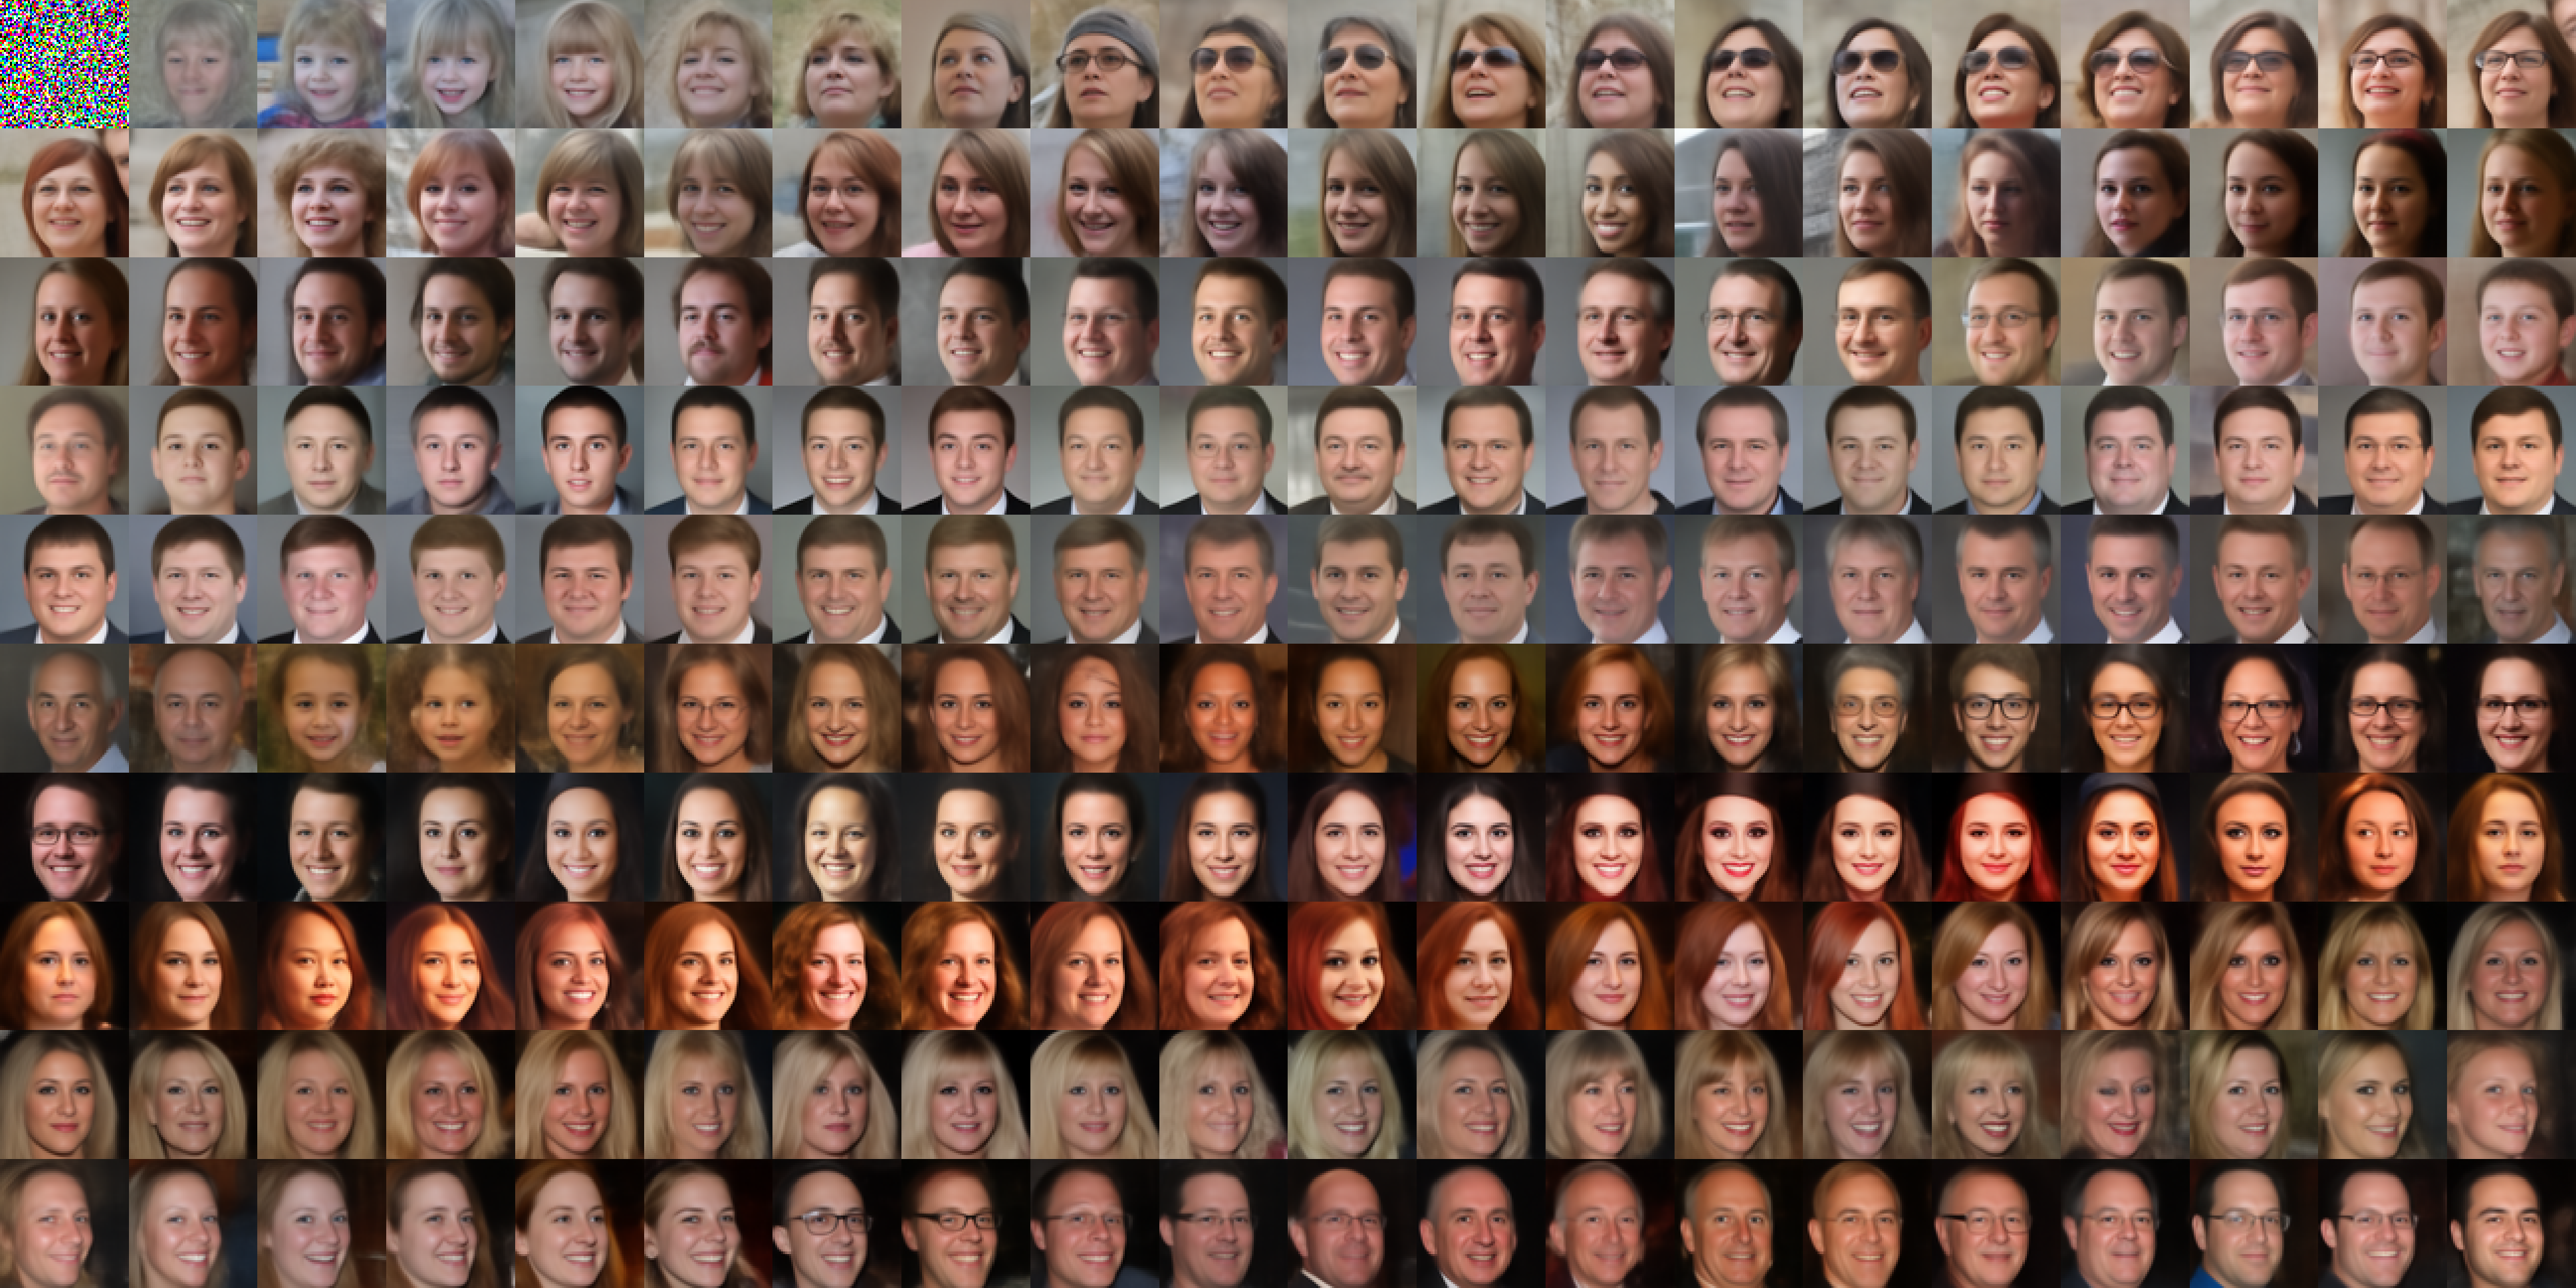
\includegraphics[width=0.75\linewidth]{figures/multiprox/ffhq.png}
    \caption{A single MultiProx chain of CIFAR10, AFHQ and FFHQ 64x64.}
    \label{fig:multiprox_images}

\end{figure} 
 %Figure \ref{fig:images_2} showcases the \texttt{MultiProx} framework applied to the denoising diffusion GAN models of \cite{xiao2022tackling}.

%\begin{figure}
%    \centering
%    \includegraphics[width=0.3\linewidth]{figures/cifar10_1.jpg}
%    \includegraphics[width=0.3\linewidth]{figures/cifar10_2.jpg}
%    \includegraphics[width=0.3\linewidth]{figures/cifar10_3.jpg}\\
%    \includegraphics[width=0.9\linewidth]{figures/celeba_256.jpg}
%    \caption{CIFAR10 (FID=7.03) and CelebA 256x256 (FID=10.54) with MultiProx for Denoising Diffusion GANs}
%    \label{fig:images_2}
%\end{figure}

%\blockcomment{
%\begin{figure}
    %\centering
    %\includegraphics[width=\linewidth]{figures/denoising.pdf}
    %\caption{The proximal sampler applied to a dataset of \emph{only} 5 images.}
%\end{figure}}


%\begin{figure}
%    \centering
    %\includegraphics[width=\linewidth]{figures/moreiterationsprox.pdf}
%    \caption{Proximal sampler on 3 examples}
%\end{figure}}

\subsubsection{Graphs}
In any case, the main experimental results that are relevant for this thesis work are those on discrete distributions. Modeling and sampling from discrete distributions such as graphs is a more complicated generative learning task. We thus focused on evaluating our sampling technique on two classical graph distribution learning tasks: learning to generate novel small molecular structures using the QM9 dataset of 9-node graphs with 4 atom (node) types and 5 bond (edge) types \cite{ruddigkeit_enumeration_2012, ramakrishnan_quantum_2014}, and Community20, a toy dataset of 100 2-block SBM-sampled random graphs. Evaluation metrics for molecules include measuring the sampling rates of valid, unique, and novel molecular structures. For the simpler Community20 dataset lacking graph interpretation, one can perform Maximum Mean Discrepancy (MMD) statistical tests for the difference between sampled and true distributions of various classical graph features as before \cite{gretton_kernel_2012, liao_efficient_2019}.

Graph diffusion model experiments differ from standard practice in that the noise process and denoising model act potentially on both continuous and discrete features, where discrete features are sampled through denoising the per-class log-probability and a final argmax over all logits to sample a graph node or edge type. DiGress \cite{vignac_digress_2022}, the state-of-the-art model that we re-evaluated with MultiProx, also introduced the discrete noise process with a categorical instead of a Gaussian distribution; however, we focused on the authors' ConGress version with Gaussian continuous-space noising for consistency with other experiments. Figure \ref{fig:multiprox_qm9} visualizes the molecule graphs in an example sampled Gibbs chain. Refer to Appendix \ref{sec:appendix_multiprox_experiments} for our results on the Community20 dataset. 

\begin{figure}[H]
    \centering
    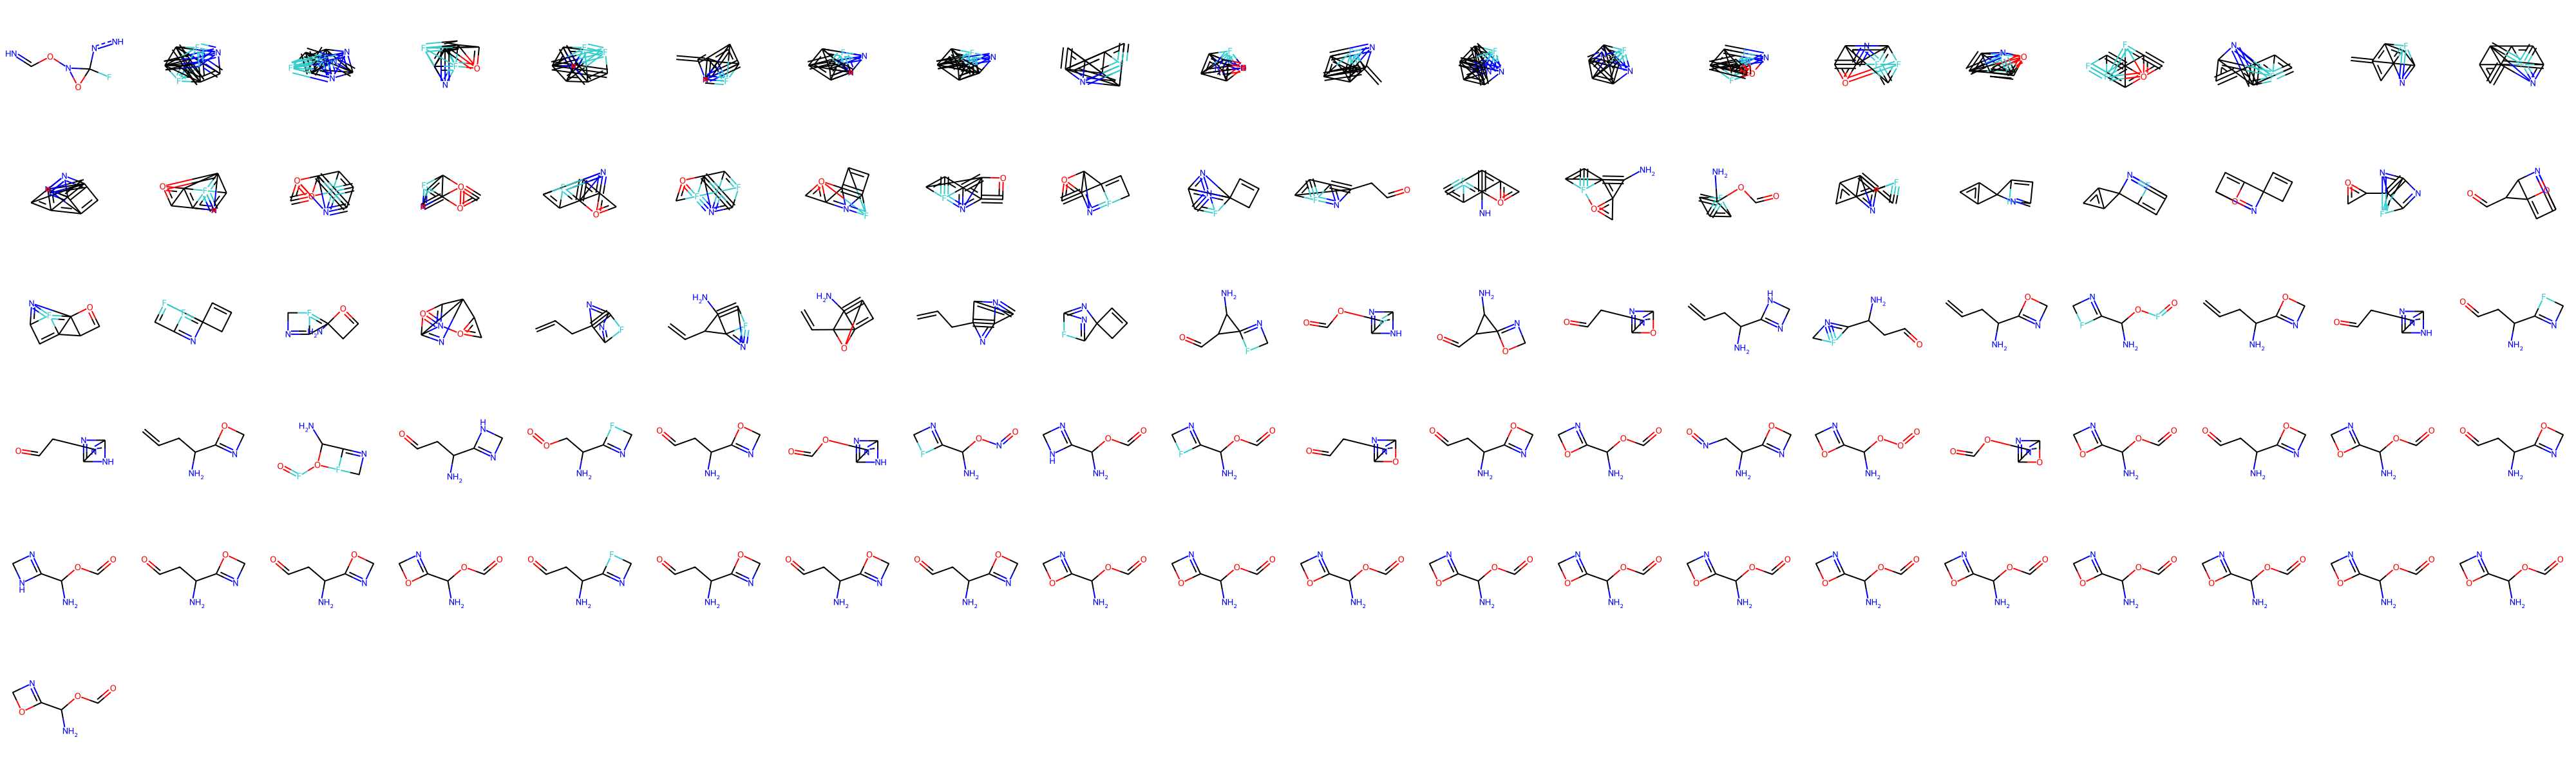
\includegraphics[width=\linewidth]{figures/multiprox/qm9_grid_image_single_noise.png}
    \caption[Best chain of molecule graphs obtained with MultiProx.]{Best chain of molecule graphs obtained with MultiProx and a ConGress denoiser. For this QM9 chain $n=10$, $m=100$, $t=50$ (10\% of $T$).
    }
    \label{fig:multiprox_qm9}
\end{figure}

From the figure, we can immediately discern issues not present in the image experiments. Namely, the warm-up phase for the molecules seems to last longer, and when it passes, the Gibbs chain seems to suffer from mode collapse relatively quickly.

Thus, when evaluating our MultiProx sampler on these discrete distributions, we observed that results could be greatly improved when adding in annealing steps before outputting the final graphs, i.e., employing the more general MultiProxAn sampler instead. The choice of moving the chain at a higher noise level $t$, then annealing to lower and lower $t'$ is empirically validated, as e.g., from Table \ref{tab:qm9_stats} one observes that this always results in more valid molecules, but nevertheless always with less compute cost when compared to the baseline. As shown by Figure \ref{fig:qm9_better}, the improvement in sample quality is also visually discernible. 

For an explanation, we hypothesize that the issue arises from the argmax projection of the Gaussian logits, which would require different guarantees on the modeling accuracy of its distribution. The higher noise level moves the Gibbs chain with a sufficiently high velocity so as to cover more modes, while the annealing steps to the lower noise level make sure there are fewer warm-up steps. We refer to the work by \cite{sahoo_diffusion_2025} for a potential solution on how to remain in the single-noise-level configuration even for complex discrete distributions. 

\begin{table}[H]
    \centering
    \caption[MultiProxAn sampling metrics for the QM9 dataset of molecule graphs.]{Sampling metrics for each noise level hyperparameter configuration we tested for the QM9 dataset of molecule graphs. Left to right: MultiProxAn fixed noise level $t$ and final output noise level $t' \leq t$ (as percentages of $T$), percentage of valid molecule graphs, percentage of unique valid molecules, percentage of novel unique valid molecules (not present in the dataset), and total execution time of sampling. Arrows indicate whether higher or lower values of a metric are better. Best values per metric are in bold, while second-best values are underlined.}
    % \resizebox{\textwidth}{!}{
    \begin{tabular}{llrrrr}
        \toprule
         $t$ & $t'$ & $\uparrow$ Valid [\%] & $\uparrow$ Unique [\%] & $\uparrow$ Novel [\%] & $\downarrow$ Wall time [s]  \\
         \midrule
         \multicolumn{2}{l}{Baseline} & \underline{96.52} & 78.34 & 54.92 & 6302 \\
         50\% & 50\% & 0.00 & 0.00 & 0.00 & \textbf{151} \\
         50\% & 25\% & 0.16 & \textbf{100.0} & \textbf{96.01} & 1655 \\
         50\% & 10\% & 74.61 & 87.74 & 66.28 & 2561 \\
         50\% & 0.4\% & \textbf{96.62} & 77.95 & 55.20 & 3137 \\
         25\% & 25\% & 0.00 & 0.00 & 0.00 & \textbf{151} \\
         25\% & 10\% & 66.62 & \underline{90.35} & 70.49 & 1056 \\
         25\% & 0.4\% & 95.29 & 77.53 & 56.10 & 1418 \\
         10\% & 10\% & 14.52 & 30.64 & \underline{95.32} & \textbf{151} \\
         10\% & 0.4\% & 64.70 & 43.38 & 85.29 & \underline{513} \\
         \bottomrule
    \end{tabular}
    % }
    \label{tab:qm9_stats}
\end{table}

\begin{figure}[H]
    \centering
    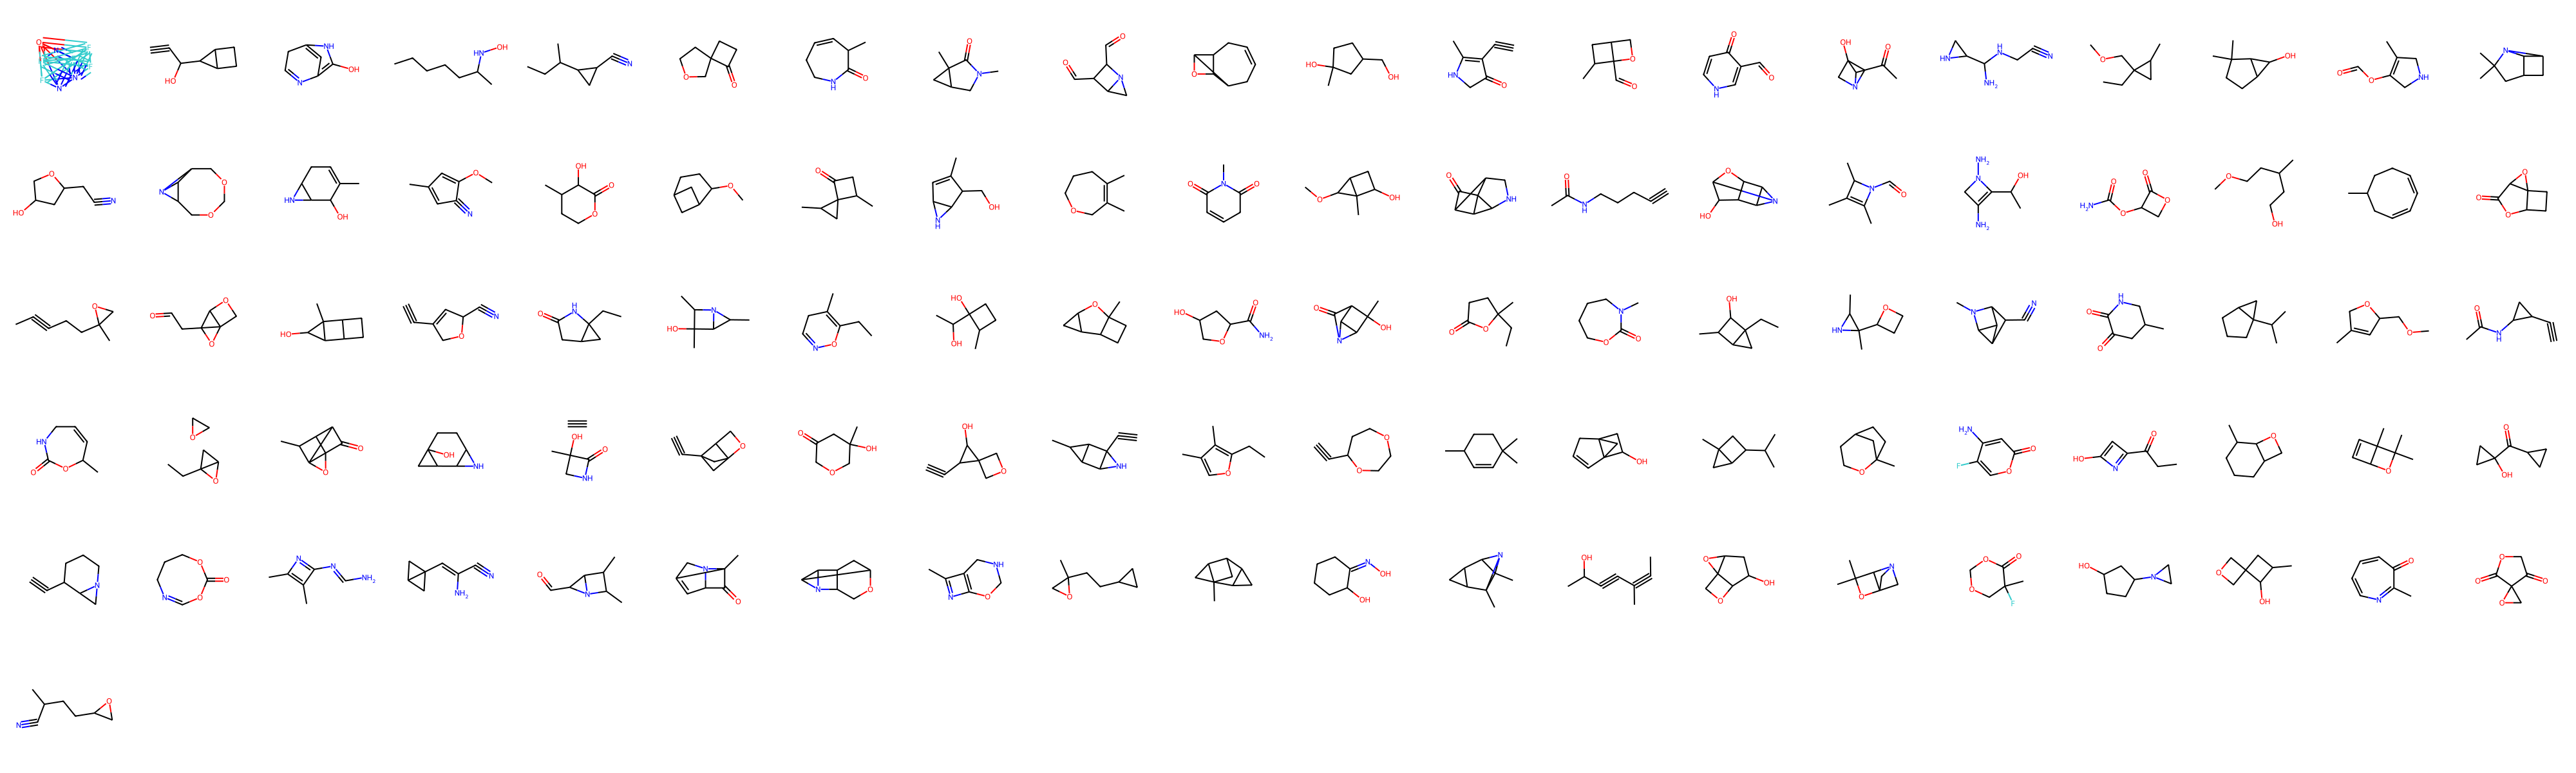
\includegraphics[width=\linewidth]{figures/multiprox/qm9_grid_image.png}
    \caption[Best chain of molecule graphs obtained with MultiProxAn.]{Best chain of molecule graphs obtained with MultiProxAn and a ConGress denoiser. For this QM9 chain $n=10$, $m=100$, $t=250$ and $t'=2$ (50\% and 0.4\% of $T$, respectively).
    }
    \label{fig:qm9_better}
\end{figure}

\subsection{Summary}

To conclude, we showed how by applying multimeasurement theory to denoising diffusion samplers, we can reproduce state-of-the-art performance metrics with much fewer denoising steps. Specifically, our MultiProxAn sampler can yield a speed-up factor of around $\frac{T}{t-t'+1}$, but experiments have shown that the values of the two fixed noise levels $t$ and $t'$ must be carefully validated. 

We again rise above purely reductionist and holistic approaches by taking a bit of each, this time to provide the best methods for sampling from multimodal distributions. We mix annealing approaches that assume it is enough to model noise step-by-step, and multimeasurement results that predict all relevant information lies in a single noise level. 

\section{Generative Knowledge Graph Anomaly Correction}
\label{sec: kg_generation}
\chapter{Conclusions \& Future Directions}
\label{chp: conclusion}

% \chapter{Introduction}


\addcontentsline{toc}{chapter}{Introduction}

\lipsum[1]
\newpage
\lipsum[5]
\newpage
\lipsum[5]
\newpage
\par
Foot note should be cited here %\footcite{REF:3}
% \chapter{Tables and Figures}
In this chapter we will see some examples of tables and figures.

\section{Tables}
Let's see how to make a well designed table.

\begin{table}[tb]
\caption[A floating table]{A floating table.}
\label{tab:esempio}
\centering
\begin{tabular}{ccc}
\toprule
name & weight & food \\ 
\midrule
mouse	& 10 g	& cheese \\
cat	& 1 kg	& mice \\
dog	& 10 kg	& cats \\
t-rex	& 10 Mg	& dogs \\
\bottomrule 
\end{tabular}
\end{table}

The table~\ref{tab:esempio} is a floating table and was obtained with the following code:
\begin{lstlisting}
\begin{table}[tb]
\caption[A floating table]{A floating table.}
\label{tab:example}
\centering
\begin{tabular}{ccc}
\toprule
	name 	& weight & food	  \\ 
\midrule
	mouse	& 10  g	 & cheese \\
	cat		&  1 kg	 & mice	  \\
	dog		& 10 kg	 & cats   \\
	t-rex	& 10 Mg	 & dogs	  \\
\bottomrule 
\end{tabular}
\end{table}
\end{lstlisting}

\lipsum[1-2]


\section{Figures}
Let's see now how to put one or several images in your text.


\begin{figure}[tb] 
\centering 
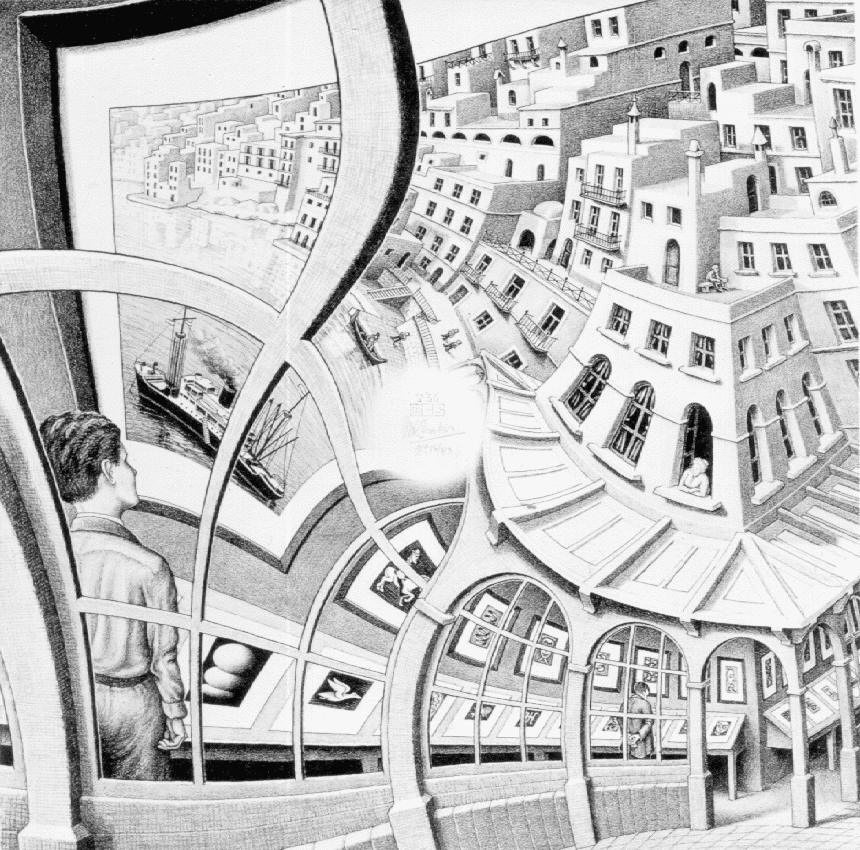
\includegraphics[width=0.5\columnwidth]{galleria_stampe} 
\caption[A floating figure]{A floating figure (the lithograph \emph{Galleria di stampe}, of M.~Escher, got from \url{http://www.mcescher.com/}).}
\label{fig:galleria} 
\end{figure}

\begin{figure}[tb] 
\centering 
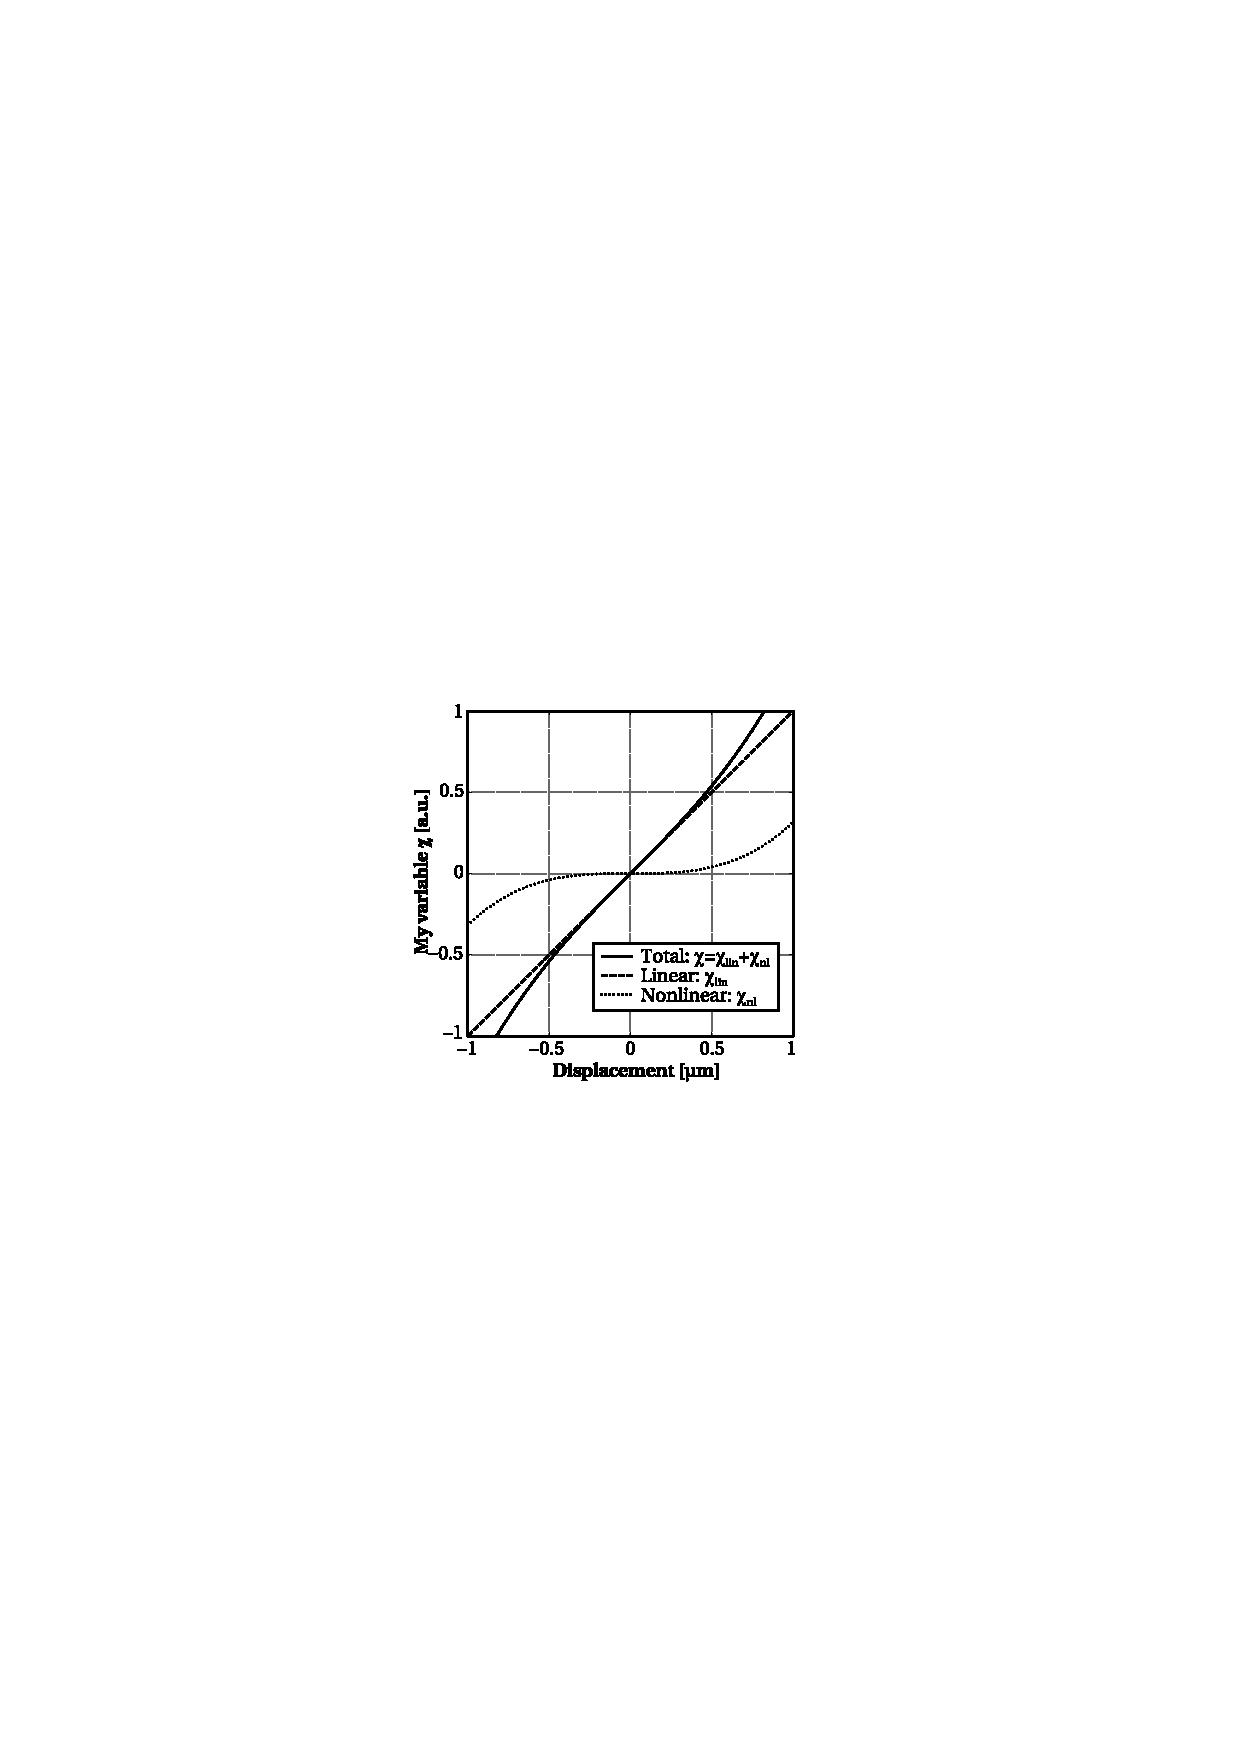
\includegraphics{some_vector_graphics.pdf} 
\caption[A floating figure]{A floating figure with text typeset in "Utopia Latex", a font provided in the template-folder for typesetting figures with greek characters. The text has been "outlined" for best compatibility with the repro during the printing.}
\label{fig:vector_graphics} 
\end{figure}


The figure~\ref{fig:galleria} is a floating figure and was obtained with the following code:
\begin{lstlisting}
\begin{figure}[tb] 
\centering 
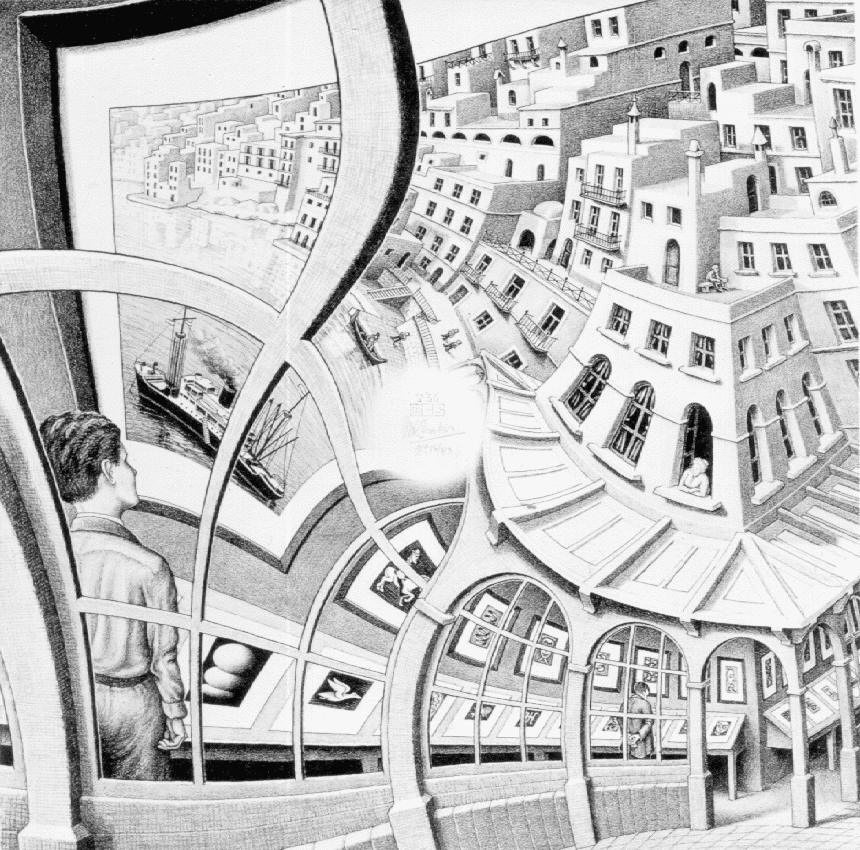
\includegraphics[width=0.5\columnwidth]{galleria_stampe} 
\caption[A floating figure]{A floating figure ... }
\label{fig:galleria} 
\end{figure}
\end{lstlisting}


\lipsum[1-2]

\begin{figure}[tb]
\centering

\subfloat[Asia personas duo.]
{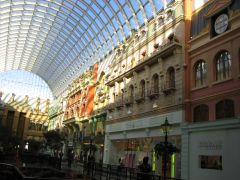
\includegraphics[width=.45\columnwidth]{lorem}} \quad
\subfloat[Pan ma signo.]
{\label{fig:ipsum}%
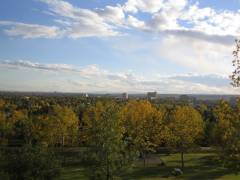
\includegraphics[width=.45\columnwidth]{ipsum}} \\
\subfloat[Methodicamente o uno.]
{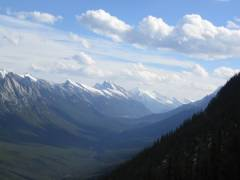
\includegraphics[width=.45\columnwidth]{dolor}} \quad
\subfloat[Titulo debitas.]
{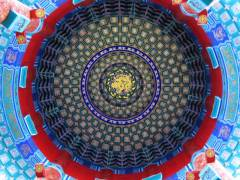
\includegraphics[width=.45\columnwidth]{sit}}
\caption[Tu duo titulo debitas latente]{Tu duo titulo debitas
latente.}
\label{fig:esempio}
\end{figure}

The figure~\ref{fig:esempio} is a floating figure and was obtained with the following code:
\begin{lstlisting}
\begin{figure}[tb]
\centering
\subfloat[Asia personas duo.]
{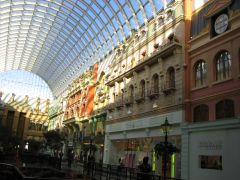
\includegraphics[width=.45\columnwidth]{lorem}} \quad
\subfloat[Pan ma signo.]
{\label{fig:ipsum}%
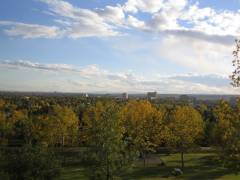
\includegraphics[width=.45\columnwidth]{ipsum}} \\
\subfloat[Methodicamente o uno.]
{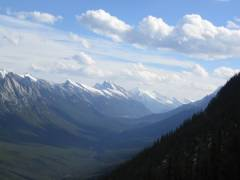
\includegraphics[width=.45\columnwidth]{dolor}} \quad
\subfloat[Titulo debitas.]
{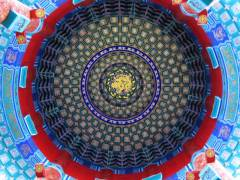
\includegraphics[width=.45\columnwidth]{sit}}
\caption[Tu duo titulo debitas latente]{Tu duo titulo debitas latente.}
\label{fig:esempio}
\end{figure}
\end{lstlisting}


\lipsum[3-8]

% \chapter{Mathematics}
In this chapter we will see some examples of mathematics.

\lipsum[1]

\section{Very important formulas}
\lipsum[2]

\begin{equation}\label{eqn:rate_eqns}
\frac{\textrm{d}}{\textrm{d}t}\left[
\begin{array}{l}
P_{\textit{0}} \\
P_{\textit{1}} \\
P_{\textit{T}}
\end{array}
\right] =
\left[
\begin{array}{l}
\frac{P_{\textit{1}}}{\tau_{\textit{10}}} + \frac{P_{\textit{T}}}{\tau_{\textit{T}}} - \frac{P_{\textit{0}}}{\tau_{\textit{ex}}} \\
- \frac{P_{\textit{1}}}{\tau_{\textit{10}}} - \frac{P_{\textit{1}}}{\tau_{isc}} + \frac{P_{\textit{0}}}{\tau_{\textit{ex}}} \\
\frac{P_{\textit{1}}}{\tau_{isc}} -  \frac{P_{\textit{T}}}{\tau_{\textit{T}}}
\end{array}
\right]
\end{equation}

\lipsum[3]


\begin{equation}\label{eqn:avgfluorescence}
\bar{I_{f}}(\vec{r})	 
	= \gamma(\vec{r}) \left(1 - \frac{\tau_{\textit{T}} P_{\textit{T}}^{{eq}}\left(1-\exp \left(-\frac{(T_p - t_p)}{\tau_{\textit{T}}}\right)\right)}{1-\exp\left(-\frac{(T_p - t_p)}{\tau_{\textit{T}}} + k_{\textit{2}} t_p\right)} \times \frac{\left(\exp\left(k_{\textit{2}} t_p\right)-1\right)}{t_p} \right) 
\end{equation}

\lipsum[3]

% \chapter{Yet another chapter}
Here you can see a citation: \cite{atc13}.

\newpage

bla bla bla bla
\newline~\newline
\lipsum[7]
\newpage
blaaa
% \chapter{The others (\textit{not the movie})}
\section{Useful stuff for citation}
\par
This is to cite stuff in-line \verb*|cite{bla-bla}| $\xrightarrow{}$ \cite{REF:3, REF:1}, but to put citations in brackets should appear something like dis \verb*|autocite{bla-bla}| $\xrightarrow{}$ \autocite{REF:3, REF:1}.
\par
Now for brief foot citations we do it like dis by using biblatex package \verb*|footcite{bla-bla}| $\xrightarrow{}$ look down\footcite{REF:1}; for fully-detailed citation we do it like dis \verb*|footfullcite{bla-bla}| $\xrightarrow{}$ look down\footfullcite{REF:1} and another one for fun\footfullcite{REF:3}.
\par
To cite the author only we do dis \verb*|citeauthor{bla-bla}| $\xrightarrow{}$ \citeauthor{REF:1}; the only year god only knows why we could use it but here we go \verb*|citeyear{bla-bla}| $\xrightarrow{}$ \citeyear{REF:1}.
\par
This is just a normal footnote \footnote{I'm just a normal footnote minding my own business}.

\section{Useful stuff chemical formulae}
\begin{itemize}
    \item The first style:\newline~\newline
\ce{Na2SO4 ->[H2O] Na+ + SO4^2-}
\ce{(2Na+,SO4^2- ) + (Ba^2+, 2Cl- ) -> BaSO4 v + 2NaCl}
~\newline~\newline
\item The second style:\newline~\newline
\begin{chemmath}
  Na_{2}SO_{4}
  \reactrarrow{0pt}{1.5cm}{\ChemForm{H_2O}}{}
  Na^{+} + SO_{4}^{2-}
\end{chemmath}
\begin{chemmath}
  (2 Na^{+},SO_{4}^{2-}) + (Ba^{2+},2 Cl^{-})
  \reactrarrow{0pt}{1cm}{}{}
  BaSO_{4} + 2 NaCl
\end{chemmath}
~\newline~\newline
\item The third style:\newline~\newline
\schemestart
\chemfig{Na_2SO_4}
\arrow{->[\footnotesize\chemfig{H_2O}]}
\chemfig{Na^+}\+\chemfig{SO_2^{-}}
\schemestop
\schemestart
(2\chemfig{Na^+}, \chemfig{SO_4^{2-}})
\+
(\chemfig{Ba^{2+}}, 2\chemfig{Cl^{-}})
\arrow(.mid east--.mid west)
\chemname[1pt]{\chemfig{BaSO_4}}{\chemfig{-[,0.75]-[5,.3,,,-stealth]}}\+2\chemfig{NaCl}
\schemestop

\end{itemize}

\newpage
just an empty page \dots

%%%%%%%%%%%%%%%%%%%%%%%%%%%%%%%%%%%%%%%%%%%%%%
%%%%% TAIL: Bibliography, Appendix, CV
%%%%%%%%%%%%%%%%%%%%%%%%%%%%%%%%%%%%%%%%%%%%%%
\appendix
\chapter{Appendix for COINs}

\section{Theory}
\label{sec:appendix_proofs}

\begin{proof}[Proposition~\ref{proposition:complexity}]
    The time complexity of the first node group prediction step of the new evaluation procedure, is proportional to the number of groups $K$, as this is the number of embeddings required. On the other hand, the second step requires as many model evaluations as the number of nodes in the group, $\abs{C_k}$. For each sample, the total is thus $K+\abs{C_k}$, while each node group is represented by $N_k^{\text{test}}$ samples in the test data. By summing over all groups $k$ one obtains the provided exact complexity.

    Regarding the expression $\sum_{k=1}^{K}{\of{K+\abs{C_k}}N_k^{\text{test}}}$, let us first assume that we have fixed the number of groups $K$ to some value in $\offf{1,\dots,\abs{V}}$ and we are aiming to optimize the distribution of nodes and evaluation samples across groups for this fixed $K$. Using the KKT theorem, one can prove that extremal configurations only occur when all groups are of equal size and/or all groups are represented with an equal amount of samples in the evaluation set. Lemma~\ref{lemma:kkt_evaluation_cost} gives the details. It is easier to strive towards $\abs{C_k} \approx \frac{\abs{V}}{K}$, however, in any case, the number of node embedding computations will then equal $N\of{K + \frac{\abs{V}}{K}}$. 
    
    To conclude, we prove that the value of $K$ is what decides whether the lower or upper bound stated above is achieved: $K=\sqrt{V}$ gives the motivating lower bound, while $K \in \offf{1, \abs{V}}$ produces the worst performance, which is in the same order as the baseline $N \abs{V}$. Lemma~\ref{lemma:min_max_evaluation_cost} gives the details.
\end{proof}

\begin{lemma}
    \label{lemma:kkt_evaluation_cost}
    Let $\offf{a_k}_{k=1}^{K}=\offf{\abs{C_k}}_{k=1}^{K}$ and $\offf{b_k}_{k=1}^{K}=\offf{N_k^{\text{test}}}_{k=1}^{K}$ denote the learnable parameters. Then with the constraints $$\sum_{k=1}^{K}{a_k}=\abs{V}, \sum_{k=1}^{K}{b_k}=N, \forall k, a_k > 0, b_k \geq 0,$$ the only extremal points of $g\of{\offf{a_k},\offf{b_k}}=\sum_{k=1}^{K}{\of{K + a_k}b_k}$ are $\forall k, a^*_k = \frac{\abs{V}}{K}$ and/or $\forall k, b^*_k = \frac{N}{K}$, with the extreme value of $g\of{\offf{a^*_k},\offf{b^*_k}}=N\of{K + \frac{\abs{V}}{K}}$.
\end{lemma}
    \begin{proof}
        The Lagrangian of the optimization problem is the following:
        \begin{align*}
             L\of{\offf{a_k},\offf{b_k}} &= \sum_{k=1}^{K}{\of{K + a_k}b_k} + \lambda_1 \of{\sum_{k=1}^{K}{a_k} - \abs{V}} + \lambda_2 \of{\sum_{k=1}^{K}{b_k} - N} \\
             &- \sum_{k=1}^{K}{\mu_k a_k} - \sum_{k=1}^{K}{\nu_k b_k}
        \end{align*}
        $$$$
    From the stationarity KKT conditions:
    \begin{align*}
        \forall k, \frac{\partial L}{\partial a_k} &= 0 \Leftrightarrow \forall k, b_k + \lambda_1 - \mu_k = 0 \Leftrightarrow  \forall k, b_k = \mu_k - \lambda_1 \\
        \forall k, \frac{\partial L}{\partial b_k} &= 0 \Leftrightarrow \forall k, a_k + K + \lambda_2 - \nu_k = 0, \Leftrightarrow \forall k, a_k = \nu_k - \lambda_2 - K
    \end{align*}
    Now, by the primal equality constraints:
    \begin{align*}
        \sum_{k=1}^{K}{a_k} &= \abs{V} \Leftrightarrow \sum_{k=1}^{K}{\of{\nu_k - \lambda_2 - K}} = \abs{V} \Leftrightarrow \lambda_2 = \frac{1}{K} \sum_{k=1}^{K}{\nu_k} - \frac{\abs{V}}{K} - K \\
        \Rightarrow \forall k, a_k &= \nu_k - \frac{1}{K} \sum_{j=1}^{K}{\nu_j} + \frac{\abs{V}}{K} \\
        \sum_{k=1}^{K}{b_k} &= N \Leftrightarrow \sum_{k=1}^{K}{\of{\mu_k - \lambda_1}} = N \Leftrightarrow \lambda_1 = \frac{1}{K} \sum_{k=1}^{K}{\mu_k} - \frac{N}{K} \\
        \Rightarrow \forall k, b_k &= \mu_k - \frac{1}{K} \sum_{j=1}^{K}{\mu_j} + \frac{N}{K}
    \end{align*}
    Finally, by the complementary slackness KKT conditions, primal inequality constraints, and dual feasibility KKT conditions:
    \begin{align*}
        \sum_{k=1}^{K}{\mu_k a_k} &= 0 \Leftrightarrow \forall k, \mu_k = 0 \Rightarrow \forall k, b^*_k=\frac{N}{K} & \text{ as $\forall k, a_k>0,\mu_k \geq 0$}\\
        \sum_{k=1}^{K}{\nu_k b_k} &= 0 \Leftarrow \forall k, \nu_k = 0 \Rightarrow \forall k, a^*_k = \frac{\abs{V}}{K} & \text{ as $\forall k, b_k \geq 0,\nu_k \geq 0$}
    \end{align*}
    \end{proof}

\begin{lemma}
    \label{lemma:min_max_evaluation_cost}
    By choosing $K=\sqrt{\abs{V}}$, one achieves the minimal evaluation cost $2 N \sqrt{\abs{V}}$, while with $K \in \offf{1, \abs{V}}$ one achieves the maximum $N\of{\abs{V} + 1}$.
\end{lemma}
\begin{proof}
    Let $f\of{K} = N\of{K + \frac{\abs{V}}{K}}$. Then note that $f'\of{K} = N - \frac{N \abs{V}}{K^2}$. From this, we find the only critical point of $f$ in $\of{1, \abs{V}}$: 
    
    $N - \frac{N \abs{V}}{K^2} = 0 \Leftrightarrow K^2 = \frac{N \abs{V}}{N} \Leftrightarrow K = \sqrt{\abs{V}}$. 
    
    Now $f''\of{K}=\frac{2 N \abs{V}}{K^3}$. As $\forall K \in \off{1, \abs{V}}, f''\of{K} > 0$, $f$ is a convex function for all values of $K$. Thus, $\sqrt{\abs{V}}$ will be both a local and global minimum, while the endpoints of the interval will be global maxima, as $\forall K \neq \sqrt{\abs{V}}, f'\of{K} > 0$, i.e., $f$ increases away from the minimum in both directions.
\end{proof}


\begin{proposition}
    \label{proposition:condition_applicability}
    Let $C \in \offf{1,\dots,K}$ be a r.v. storing from which community a sample belongs. Let $\forall k \in \offf{1,\dots,K}, H'_k \in \offf{1,\dots\,\abs{C_k}}$ be the r.v. counting how many samples need to be evaluated before a correct hit in community $k$ is achieved by COINs, with $\forall k, H_k$ counting the same for the baseline model. 
    
    Let $\forall k, T'_k=K+\abs{C_k}$ denote the number of embedding computations required for evaluating a sample in community $k$ (recall Proposition~\ref{proposition:complexity}), with $T_k=\abs{V}$ counting the same for the baseline model. 
    
    Let $\forall k, \bar{\rho}'_k$ be the evaluated mean rank for samples from community $k$ for COINs, with $\bar{\rho}$ denoting the baseline mean rank. 
    
    Finally, let $\forall k, \varepsilon_k = \frac{\bar{\rho}'_k - \bar{\rho}}{\bar{\rho}}$ denote the per-community relative error in mean rank incurred to the baseline after training and evaluating the model with COINs, while let $\forall k, A_k=\frac{T_k}{T'_k}=\frac{\abs{V}}{K+\abs{C_k}}$ denote the per-community acceleration achieved. 
    
    Then, if we assume that:
    \begin{itemize}
        \item $\forall k, \mathbb{P}\of{C=k}=\frac{N_k^{\text{test}}}{N}$, and
        \item $\forall j \in \offf{1,\dots\,\abs{C_k}}, \mathbb{P}\of{H_k \leq j}=\of{\text{Hits@j}}_k$,
    \end{itemize}
     the application of COINs is justified if:
    \begin{equation}
        \label{eq:condition_applicability}
        \sum_{k=1}^{K}{\frac{N_k^{\text{test}}}{N} \frac{1 + \varepsilon_k}{A_k}} < 1
    \end{equation}
\end{proposition}
\begin{proof}
The better model is deemed the one with lower overall expected cost up until a correct hit:
    \begin{align*}
        \mathbb{E}\off{T' H'} &< \mathbb{E}\off{T H} \\
        \Leftrightarrow \sum_{k=1}^{K}{\frac{N_k^{\text{test}}}{N} T'_k \bar{\rho}'_k} &< T \bar{\rho}, & \text{ by Lemma~\ref{lemma:expected_evaluations}} \\
        \Leftrightarrow \sum_{k=1}^{K}{\frac{N_k^{\text{test}}}{N} \frac{1 + \varepsilon_k}{A_k}} &< 1, & \text{ after dividing by RHS}
    \end{align*}
\end{proof}%

\begin{lemma}
    \label{lemma:expected_evaluations}
    Let $C \in \offf{1,\dots,K}$ be a r.v. storing from which community a sample belongs. Let $H$ be the r.v. counting how many queries were evaluated before a correct hit is achieved and let $F$ denote the r.v. counting the number of embedding computations required for evaluating a sample. Then:
    $$\mathbb{E}\off{T H} = \sum_{k=1}^{K}{\frac{N_k^{\text{test}}}{N} T_k \bar{\rho}_k}$$
\end{lemma}
\begin{proof}
    \begin{align*}
        &\mathbb{E}\off{T H} = \mathbb{E}_{C}\off{\mathbb{E}\off{T H \mid C}}%, & \text{ by the Law of Total Expectation} 
        %\\
        %&
        = \sum_{k=1}^{K}{\mathbb{E}\off{T H \mid C=k} \mathbb{P}\of{C=k}}%, & \text{ by definition and the LOTUS} 
        \\
        &= \sum_{k=1}^{K}{T_k \mathbb{E}\off{H_k} \mathbb{P}\of{C=k}}%, & \text{ by definition and linearity of exp.} 
        %\\
        %&
        = \sum_{k=1}^{K}{\mathbb{P}\of{C=k} T_k \sum_{j=1}^{\abs{C_k}}{j \mathbb{P}\of{H_k=j}}}%, & \text{ by definition} 
        \\
        &= \sum_{k=1}^{K}{\mathbb{P}\of{C=k} T_k \sum_{j=1}^{\abs{C_k}}{j \off{\mathbb{P}\of{H_k \leq j} - \mathbb{P}\of{H_k \leq j-1}}}}%, & \text{ since $H_k$'s are discrete r.v.s} 
        \\
        &= \sum_{k=1}^{K}{\mathbb{P}\of{C=k} T_k \off{\abs{C_k}- \sum_{j=1}^{\abs{C_k}-1}{\mathbb{P}\of{H_k \leq j}}}}%, & \text{ after cancelling out the telescoping} 
        \\
        &= \sum_{k=1}^{K}{\frac{N_k^{\text{test}}}{N} T_k \off{\abs{C_k}- \sum_{j=1}^{\abs{C_k}-1}{\of{\text{Hits@j}}_k}}}%, & \text{ by the assumptions} 
        \\
        &= \sum_{k=1}^{K}{\frac{N_k^{\text{test}}}{N} T_k \off{\abs{C_k}- \sum_{j=1}^{\abs{C_k}-1}{\frac{1}{N_k^{\text{test}}}\sum_{i \mid c\of{a_i}=k}{\mathbb{I}\of{\rho^{\of{i}} \leq j}}}}}%, & \text{ by definition} 
        \\
        &= \sum_{k=1}^{K}{\frac{N_k^{\text{test}}}{N} T_k \off{\abs{C_k}- \frac{1}{N_k^{\text{test}}}\sum_{i \mid c\of{a_i}=k}{\of{\abs{C_k}- \rho^{\of{i}}}}}}%, & \text{ after switching sum order} 
        \\
        &= \sum_{k=1}^{K}{\frac{N_k^{\text{test}}}{N} T_k \off{\abs{C_k}- \abs{C_k} + \frac{1}{N_k^{\text{test}}}\sum_{i \mid c\of{a_i}=k}{\rho^{\of{i}}}}}%, & \text{ after distributing} 
        \\
        % &= \sum_{k=1}^{K}{\frac{N_k^{\text{test}}}{N} T_k \off{\abs{C_k}- \abs{C_k} + \bar{\rho}_k }}, & \text{ by definition} \\
        &= \sum_{k=1}^{K}{\frac{N_k^{\text{test}}}{N} T_k \bar{\rho}_k}%, & \text{ by definition}
    \end{align*}
    If $\forall k, T_k = T$ like for the baseline models, then:
    \begin{align*}
        \mathbb{E}\off{T H} &= T \sum_{k=1}^{K}{\frac{N_k^{\text{test}}}{N} \bar{\rho}_k}%, & \text{ by linearity of expectation and everything before} 
        %\\ 
        %&
        = T \sum_{k=1}^{K}{\frac{N_k^{\text{test}}}{N} \frac{1}{N_k^{\text{test}}}\sum_{i \mid c\of{a_i}=k}{\rho^{\of{i}}}}%, & \text{ by definition} 
        \\
        &= T \frac{1}{N} \sum_{i=1}^{N}{\rho^{\of{i}}}%, & \text{ after cancelling and combining the sums} 
        %\\
        %&
        = T \bar{\rho}%, & \text{ by definition}
    \end{align*}
\end{proof}

\begin{proof}[Proposition \ref{proposition:complexity_distributed}]
    To explain the complexity, we note that in a parallel computing setting, where we assume equal computation power for each machine, the overall cost of Step 2 is equal to that of the machine who will do the most work (in this case the most node-level query-answer embeddings computed). The additional $KN$ term is the total cost of Step 1, which is not parallelized.

    The largest overall cost is naturally achieved when $\abs{U}=1$, i.e. we fall back to the single-machine setting without parallelization, thus the upper bound is the same as before.

    The lower bound requires a new argument based on calculus. To start, the obvious lower bound to the maximum cost across machines is the minimum cost. We would achieve this lower bound when the max and min are equal, i.e. only when each machine does the same amount of work. In our case, this quantity is $\textcolor{blue}{\frac{1}{\abs{U}}}\sum_{k=1}^{K}{\abs{C_k}N_k^{\text{test}}}$. If we keep $\abs{U}$ and $K$ fixed as constants, we can use the KKT result from the proof of Proposition \ref{proposition:complexity} and deduce that now the only extremal points will have the form $N\of{K+\frac{\abs{V}}{K\textcolor{blue}{\abs{U}}}}$. Note that we have the constraints $1 \leq K \leq \abs{V}$ and $1 \leq \abs{U} \leq K$ (having more machines than communities is useless).

    Let $f\of{K, \abs{U}}=N\of{K+\frac{\abs{V}}{K\abs{U}}}$. Then $\nabla f \of{K, \abs{U}}=\of{\frac{\partial f}{\partial K},\frac{\partial f}{\partial \abs{U}}}=\of{N\of{1-\frac{\abs{V}}{K^2\abs{U}}}, -N\frac{\abs{V}}{K\abs{U}^2}})$.

    Setting $\nabla f = \of{0, 0}$ yields that we must have $K^2\abs{U}=\abs{V}$ and $K\abs{U}^2 \to \infty$, which is impossible with the constraints. So the only critical points can be boundary points:
    \begin{itemize}
        \item The corners $\offf{\of{1, 1}, \of{\abs{V}, 1}, \of{\abs{V},\abs{V}}}$;
        \item On the line $\abs{U}=1$, we know $K=\sqrt{\abs{V}}$ is a local minimum;
        \item On the line $K=\abs{V}$, $f\of{K, \abs{U}}=N\of{\abs{V}+\frac{1}{\abs{U}}}$ simply monotonically decreases with $\abs{U}$, so there is no local minimum on this line;
        \item On the line $\abs{U}=K$, $f\of{K, \abs{U}}=N\of{K+\frac{\abs{V}}{K^2}}$. So $\frac{d f}{d K}=N\of{1-\frac{2\abs{V}}{K^3}}$. Setting $\frac{d f}{d K}=0$ yields the local minimum $K=\sqrt[3]{2\abs{V}}$ on this line.
    \end{itemize}
    So the full set of global minimum candidates is: $$\of{K^*, \abs{U}^*} \in \offf{\of{1, 1}, \of{\abs{V}, 1}, \of{\abs{V},\abs{V}}, \of{\sqrt{\abs{V}}, 1}, \of{\sqrt[3]{2\abs{V}}, \sqrt[3]{2\abs{V}}} }.$$ Out of all of them, using both $\sqrt[3]{2\abs{V}}$ communities and machines yields the minimal function value of $\frac{3}{2}N\sqrt[3]{2\abs{V}}$.
\end{proof}

\section{Balanced Partitioning for Distributed COINs}
\label{sec:appendix_balanced_partition_algs}

Algorithm \ref{algorithm:balanced_partition} details the optimal solution to the balanced partition problem using top-down dynamic programming, while Algorithm \ref{algorithm:balanced_partition_greedy} displays the scalable greedy method.

\begin{algorithm}[H]
\algsetup{linenosize=\tiny}
\scriptsize
\caption{Exact Balanced Partition}
\label{algorithm:balanced_partition}
\begin{algorithmic}[1]
\STATE{\textbf{input} $\offf{p_k}_{k=1}^{K+1}$, $U=\offf{u_1,u_2,\dots}$}
\STATE{$S \gets \sum_{k=1}^{K+1}{p_k}$}
\STATE{MEMO$\gets\offf{}$}
\STATE{\textbf{function} $\text{MinCost}\of{k,\offf{s_j}_{j=1}^{\abs{U}-1}}$:}
% \bindent
\IF{$\of{k,\offf{s_j}_{j=1}^{\abs{U}-1}}\notin$ MEMO}
% \bindent
\IF{$k=K+2$}
% \bindent
\STATE{$\mu\gets\max\of{\max_{j=1}^{\abs{U}-1}{s_j},S-\sum_{j=1}^{\abs{U}-1}{s_j}}$}
% \eindent
\ELSE
% \bindent
\STATE{$\mu\gets\text{MinCost}\of{k+1,\offf{s_j}_{j=1}^{\abs{U}-1}}$}
\FOR{$i \leftarrow 1$ to $\abs{U}-1$}
% \bindent
\STATE{$\mu\gets\min\of{\mu, \text{MinCost}\of{k+1,\offf{s_j}_{j=1}^{i-1}\cup\offf{s_i+p_k}\cup\offf{s_j}_{j=i+1}^{\abs{U}-1}}}$}
% \eindent
\ENDFOR
% \eindent
\ENDIF
% \eindent
\STATE{MEMO$\off{\of{k,\offf{s_j}_{j=1}^{\abs{U}-1}}}\gets\mu$}
\ENDIF
\RETURN{MEMO$\off{\of{k,\offf{s_j}_{j=1}^{\abs{U}-1}}}$}
% \eindent
\STATE{\textbf{end} MinCost}
\STATE{$\mu^*\gets$MinCost$\of{1, \offf{0}_{j=1}^{\abs{U}-1}}$}
\STATE{$\offf{s^*_j}_{j=1}^{\abs{U}-1}\gets\offf{0}_{j=1}^{\abs{U}-1}$}
\FOR{$k \leftarrow 1$ to $K+1$}
\STATE{$i^*\gets\abs{U}$}
\FOR{$i \leftarrow 1$ to $\abs{U}-1$}
\IF{MEMO$\off{\of{k+1, \offf{s^*_j}_{j=1}^{i-1}\cup\offf{s^*_j+p_k}\cup\offf{s^*_j}_{j=i+1}^{\abs{U}-1}}}=\mu^*$}
\STATE{$i^*\gets i$}
\ENDIF
\ENDFOR
\STATE{$s_{i^*}^*\gets s_{i^*}^*+p_k$}
\IF{$k=K+1$}
\STATE{$u\of{g_V^*}\gets u_{i^*}$}
\ELSE
\STATE{$u\of{g_V^k}\gets u_{i^*}$}
\ENDIF
\ENDFOR
\end{algorithmic}
\end{algorithm}

\begin{algorithm}[H]
% \algsetup{linenosize=\tiny}
% \scriptsize
\caption{Greedy Balanced Partition}
\label{algorithm:balanced_partition_greedy}
\begin{algorithmic}[1]
\STATE{\textbf{input} $\offf{p_k}_{k=1}^{K+1}$, $U=\offf{u_1,u_2,\dots}$}
\STATE{$h_C\gets\text{MaxHeap}\of{\offf{\of{p_k,k}}_{k=1}^{K+1}}$}
\STATE{$h_U\gets\text{MinHeap}\of{\offf{\of{0,j}}_{j=1}^{\abs{U}}}$}
\FOR{$l \leftarrow 1$ to $K+1$}
\STATE{$\of{p_k^*,k^*}\gets\text{HeapPop}\of{h_C}$}
\STATE{$\of{s_i^*,i^*}\gets\text{HeapPop}\of{h_U}$}
\IF{$k^*=K+1$}
\STATE{$u\of{g_V^*}\gets u_{i^*}$}
\ELSE
\STATE{$u\of{g_V^{k^*}}\gets u_{i^*}$}
\ENDIF
\STATE{$\text{HeapPush}\of{h_U,\of{s_i^*+p_k^*,i^*}}$}
\ENDFOR
\end{algorithmic}
\end{algorithm}


\section{Hyperparameters}
\label{sec:appendix_hpars}

Table~\ref{tab:hyperparameters} lists the chosen values of the main hyperparameters influencing community detection, model architecture and optimization.

\begin{table}[ht!]
  \caption[COINs hyperparameter configurations.]{COINs hyperparameter configurations. Left to right: Leiden resolution, embedding dimension, contrastive loss margin, COINs loss weight, mini-batch size, number of negative samples per positive, total number of training epochs, learning rate, and regularization weight.}
  \label{tab:hyperparameters}
  \centering
  \begin{tabular}{llccccccccc}
    \toprule
    Dataset & Model & resolution & $D$ & $\gamma$ & $\alpha$ & $B$ & $m$ & ep. & l.r. & $\lambda$ \\
    \midrule
\multirow{6}{*}{FB15k-237} & TransE & $5 \cdot 10^{-3}$ & 100 & 1.0 & 0.5 & 256 & 128 & 5 & $10^{-3}$ & $10^{-6}$ \\
 & DistMult & $5 \cdot 10^{-3}$ & 100 & \textemdash & 0.5 & 256 & 128 & 50 & $10^{-3}$ & $10^{-6}$ \\
 & ComplEx & $5 \cdot 10^{-3}$ & 100 & \textemdash & 0.5 & 256 & 128 & 50 & $10^{-3}$ & $10^{-6}$ \\
 & RotatE & $5 \cdot 10^{-3}$ & 100 & 9.0 & 0.5 & 256 & 128 & 5 & $10^{-3}$ & $10^{-6}$ \\
 & KBGAT & $5 \cdot 10^{-3}$ & 100 & 9.0 & 0.5 & 256 & 128 & 50 & $10^{-3}$ & $10^{-6}$ \\
  & Query2Box & $5 \cdot 10^{-3}$ & 400 & 24.0 & 0.5 & 256 & 128 & 35 & $10^{-4}$ & $10^{-6}$ \\
\midrule
\multirow{6}{*}{WN18RR} & TransE & $2.4 \cdot 10^{-5}$ & 100 & 1.0 & 0.5 & 256 & 128 & 20 & $10^{-3}$ & $10^{-6}$ \\
 & DistMult & $2.4 \cdot 10^{-5}$ & 100 & \textemdash & 0.5 & 256 & 128 & 200 & $10^{-3}$ & $10^{-6}$ \\
 & ComplEx & $2.4 \cdot 10^{-5}$ & 100 & \textemdash & 0.5 & 256 & 128 & 200 & $10^{-3}$ & $10^{-6}$ \\
 & RotatE & $2.4 \cdot 10^{-5}$ & 100 & 6.0 & 0.5 & 256 & 128 & 20 & $10^{-3}$ & $10^{-6}$ \\
 & KBGAT & $2.4 \cdot 10^{-5}$ & 100 & 6.0 & 0.5 & 256 & 128 & 200 & $10^{-3}$ & $10^{-6}$ \\
& Query2Box & $2.4 \cdot 10^{-5}$ & 400 & 24.0 & 0.5 & 256 & 128 & 140 & $10^{-4}$ & $10^{-6}$ \\
\midrule
\multirow{6}{*}{NELL-995} & TransE & $2 \cdot 10^{-5}$ & 100 & 1.0 & 0.5 & 256 & 128 & 10 & $10^{-3}$ & $10^{-6}$ \\
 & DistMult & $2 \cdot 10^{-5}$ & 100 & \textemdash & 0.5 & 256 & 128 & 100 & $10^{-3}$ & $10^{-6}$ \\
 & ComplEx & $2 \cdot 10^{-5}$ & 100 & \textemdash & 0.5 & 256 & 128 & 100 & $10^{-3}$ & $10^{-6}$ \\
 & RotatE & $2 \cdot 10^{-5}$ & 100 & 6.0 & 0.5 & 256 & 128 & 10 & $10^{-3}$ & $10^{-6}$ \\
  & KBGAT & $2 \cdot 10^{-5}$ & 100 & 6.0 & 0.5 & 256 & 128 & 100 & $10^{-3}$ & $10^{-6}$ \\
 & Query2Box & $2 \cdot 10^{-5}$ & 400 & 24.0 & 0.5 & 256 & 128 & 70 & $10^{-4}$ & $10^{-6}$ \\ 
\bottomrule
  \end{tabular}
\end{table}

\section{Additional results}
\label{sec:appendix_results}

\subsection{Communities \& Scalability}

Figure~\ref{fig:scalability_cut_size} illustrates an alternative method to optimize the scalability factors, through optimization of the cut size (number of inter-community edges) heuristic utilized by the METIS algorithm.

For Leiden, one observes smooth curves with similar properties as in Figure~\ref{fig:scalability_resolution}, where we had the resolution parameter as the independent variable. For optimal acceleration, there seems to be a critical cut size, while having more inter-community edges implied more parameters for $g^{*}_V$. 

Curiously, we observed the METIS algorithm to yield a non-minimal cut size, and there are a lot of Leiden resolution values that achieve lower cut sizes. METIS clearly favors too large of an increase in parameter number. The distribution of the metrics over a batch of 100 random uniform community assignments yielded extremal values: the best acceleration, however the largest cut size and most parameters.

\begin{figure}[H]
\begin{center}
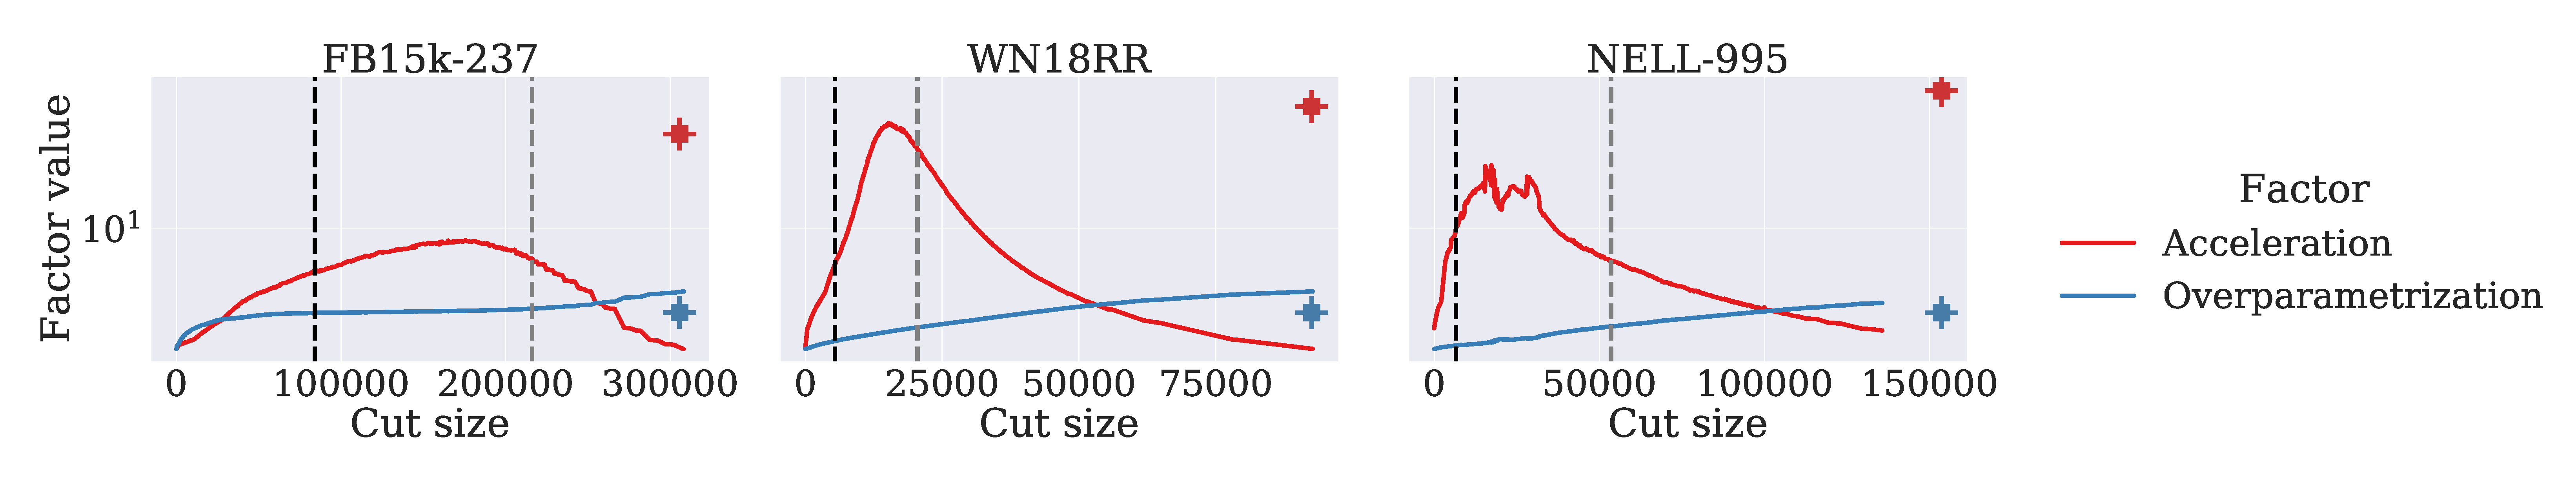
\includegraphics[width=\textwidth]{figures/coins/scalability_leiden_cut_size}
\end{center}
\caption[Dependence of time and memory scalability on the cut size of community partitions obtained by varying the resolution hyperparameter of the Leiden community detection algorithm.]{Dependence of time and memory scalability (acceleration and overparametrization factors) on the cut size (number of inter-community edges) of community partitions obtained by varying the resolution hyperparameter of the Leiden community detection algorithm. Left to right: different datasets. Cut values that yielded optimal balance between scalability and performance for each dataset annotated via black vertical lines. Gray vertical lines denote the cut size values obtained by the METIS algorithm, while the boxes with error bars denote the results from a batch of 100 random uniform community assignments.}
\label{fig:scalability_cut_size}
\end{figure}

Figure~\ref{fig:scalability_modularity} illustrates yet another alternative method to optimize the scalability factors, through optimization of the modularity heuristic utilized by the Leiden algorithm. 

In general, for Leiden, one observes both more acceleration and less overparametrization as modularity increases, however, as the plots display, we found this method to be more unstable than simply traversing the resolution hyperparameter space as before in Figure~\ref{fig:scalability_resolution}. We also note that the METIS algorithm produced slightly higher modularity only for the WN18RR dataset. Random community assignments again, naturally, yield extremal values.

\begin{figure}[H]
\begin{center}
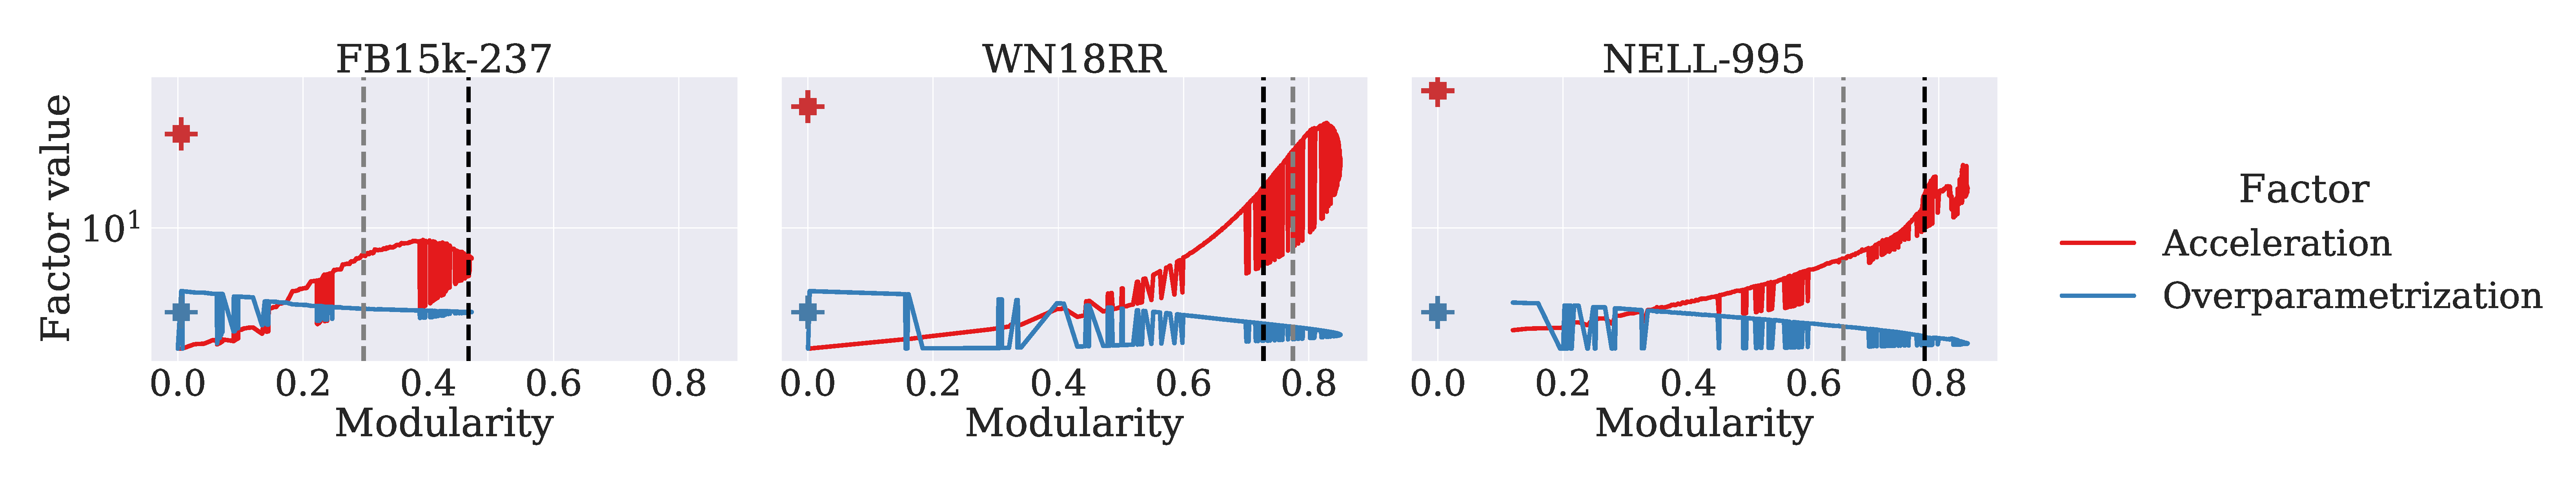
\includegraphics[width=\textwidth]{figures/coins/scalability_leiden_modularity}
\end{center}
\caption[Dependence of time and memory scalability on the value of the modularity heuristic of the Leiden community detection algorithm.]{Dependence of time and memory scalability (acceleration and overparametrization factors) on the value of the modularity heuristic of the Leiden community detection algorithm. Left to right: different datasets. Modularity values that yielded optimal balance between scalability and performance for each dataset annotated via black vertical lines. Gray vertical lines denote the modularity values obtained by the METIS algorithm, while the boxes with error bars denote the results from a batch of 100 random uniform community assignments.}
\label{fig:scalability_modularity}
\end{figure}

\subsection{Performance \& Feasibility}

Table~\ref{tab:performance_query_answering} contains our full query answering metric comparison with the baselines, while Table~\ref{tab:performance_query_answering_2} provides further insight into our query answering performance, after analyzing separately the metrics for each of the two prediction steps. We can observe how well the community Hits@1 score captures the influence of the accuracy in the community prediction on the overall performance. 

Namely, with some quick calculations, one can interestingly note that the overall COINs metric values can be closely approximated as the product of the community Hits@1 and respective scores for the within-community node prediction.

\begin{table}[!ht]
  \caption[All computed query answering metrics.]{All computed query answering metrics (higher is better): comparison of our results with COINs training and evaluation to baselines with equal hyperparameters. Values in bold indicate the superiority of COINs, while underlined values have a relative error lower than 10\%.}
  \label{tab:performance_query_answering}
  \centering
  \begin{adjustbox}{width=\textwidth}   
\begin{tabular}{llllllll}
\toprule
         &           &       &                ComHits@1 &                             Hits@1 &                             Hits@3 &                            Hits@10 &                                MRR \\
Dataset & Algorithm & Value &                          &                                    &                                    &                                    &                                    \\
\midrule
FB15k-237 & TransE & Baseline &                          &                        ${{0.142}}$ &                         ${{0.24}}$ &                        ${{0.369}}$ &                        ${{0.218}}$ \\
         &           & COINs &    ${{0.676}_{\pm 0.0}}$ &            ${{0.078}_{\pm 0.003}}$ &            ${{0.136}_{\pm 0.005}}$ &            ${{0.245}_{\pm 0.007}}$ &            ${{0.132}_{\pm 0.004}}$ \\
         & DistMult & Baseline &                          &                        ${{0.254}}$ &                        ${{0.377}}$ &                        ${{0.527}}$ &                        ${{0.344}}$ \\
         &           & COINs &  ${{0.291}_{\pm 0.045}}$ &            ${{0.038}_{\pm 0.007}}$ &            ${{0.074}_{\pm 0.012}}$ &            ${{0.132}_{\pm 0.012}}$ &            ${{0.068}_{\pm 0.009}}$ \\
         & ComplEx & Baseline &                          &                        ${{0.278}}$ &                        ${{0.404}}$ &                        ${{0.552}}$ &                        ${{0.369}}$ \\
         &           & COINs &  ${{0.975}_{\pm 0.007}}$ &     $\mathbf{{0.333}_{\pm 0.007}}$ &     $\mathbf{{0.477}_{\pm 0.007}}$ &     $\mathbf{{0.626}_{\pm 0.007}}$ &     $\mathbf{{0.431}_{\pm 0.006}}$ \\
         & RotatE & Baseline &                          &                        ${{0.282}}$ &                         ${{0.43}}$ &                        ${{0.584}}$ &                        ${{0.383}}$ \\
         &           & COINs &  ${{0.944}_{\pm 0.001}}$ &     $\mathbf{{0.295}_{\pm 0.003}}$ &  $\underline{{0.416}_{\pm 0.004}}$ &  $\underline{{0.552}_{\pm 0.004}}$ &  $\underline{{0.381}_{\pm 0.003}}$ \\
         & KBGAT & Baseline &                          &                         ${{0.46}}$ &                         ${{0.54}}$ &                        ${{0.626}}$ &                        ${{0.518}}$ \\
         &           & COINs &  ${{0.954}_{\pm 0.005}}$ &            ${{0.163}_{\pm 0.013}}$ &              ${{0.27}_{\pm 0.02}}$ &            ${{0.412}_{\pm 0.024}}$ &            ${{0.245}_{\pm 0.015}}$ \\
         & Query2Box & Baseline &                          &            ${{0.129}_{\pm 0.005}}$ &            ${{0.168}_{\pm 0.002}}$ &              ${{0.2}_{\pm 0.002}}$ &            ${{0.154}_{\pm 0.004}}$ \\
         &           & COINs &  ${{0.721}_{\pm 0.006}}$ &     $\mathbf{{0.186}_{\pm 0.002}}$ &     $\mathbf{{0.289}_{\pm 0.003}}$ &     $\mathbf{{0.402}_{\pm 0.005}}$ &     $\mathbf{{0.261}_{\pm 0.002}}$ \\
\midrule
WN18RR & TransE & Baseline &                          &                        ${{0.019}}$ &                        ${{0.241}}$ &                        ${{0.416}}$ &                         ${{0.16}}$ \\
         &           & COINs &  ${{0.941}_{\pm 0.007}}$ &     $\mathbf{{0.199}_{\pm 0.006}}$ &     $\mathbf{{0.311}_{\pm 0.008}}$ &     $\mathbf{{0.436}_{\pm 0.012}}$ &     $\mathbf{{0.278}_{\pm 0.008}}$ \\
         & DistMult & Baseline &                          &                        ${{0.399}}$ &                        ${{0.452}}$ &                        ${{0.489}}$ &                        ${{0.433}}$ \\
         &           & COINs &  ${{0.997}_{\pm 0.001}}$ &            ${{0.176}_{\pm 0.063}}$ &            ${{0.305}_{\pm 0.086}}$ &            ${{0.423}_{\pm 0.077}}$ &            ${{0.261}_{\pm 0.071}}$ \\
         & ComplEx & Baseline &                          &                        ${{0.426}}$ &                        ${{0.479}}$ &                        ${{0.526}}$ &                        ${{0.462}}$ \\
         &           & COINs &    ${{0.999}_{\pm 0.0}}$ &             ${{0.297}_{\pm 0.02}}$ &            ${{0.394}_{\pm 0.017}}$ &             ${{0.466}_{\pm 0.01}}$ &            ${{0.358}_{\pm 0.018}}$ \\
         & RotatE & Baseline &                          &                        ${{0.442}}$ &                        ${{0.491}}$ &                        ${{0.538}}$ &                        ${{0.476}}$ \\
         &           & COINs &    ${{0.998}_{\pm 0.0}}$ &  $\underline{{0.436}_{\pm 0.001}}$ &      $\mathbf{{0.51}_{\pm 0.003}}$ &     $\mathbf{{0.586}_{\pm 0.004}}$ &     $\mathbf{{0.487}_{\pm 0.001}}$ \\
         & KBGAT & Baseline &                          &                        ${{0.361}}$ &                        ${{0.483}}$ &                        ${{0.581}}$ &                         ${{0.44}}$ \\
         &           & COINs &    ${{0.998}_{\pm 0.0}}$ &            ${{0.274}_{\pm 0.005}}$ &            ${{0.404}_{\pm 0.006}}$ &             ${{0.52}_{\pm 0.006}}$ &            ${{0.359}_{\pm 0.003}}$ \\
         & Query2Box & Baseline &                          &            ${{0.187}_{\pm 0.004}}$ &            ${{0.308}_{\pm 0.001}}$ &            ${{0.385}_{\pm 0.001}}$ &             ${{0.26}_{\pm 0.001}}$ \\
         &           & COINs &  ${{0.958}_{\pm 0.018}}$ &     $\mathbf{{0.218}_{\pm 0.008}}$ &     $\mathbf{{0.382}_{\pm 0.007}}$ &     $\mathbf{{0.524}_{\pm 0.005}}$ &     $\mathbf{{0.323}_{\pm 0.007}}$ \\
\midrule
NELL-995 & TransE & Baseline &                          &                         ${{0.23}}$ &                        ${{0.368}}$ &                        ${{0.448}}$ &                        ${{0.312}}$ \\
         &           & COINs &    ${{0.971}_{\pm 0.0}}$ &             ${{0.15}_{\pm 0.011}}$ &            ${{0.244}_{\pm 0.012}}$ &            ${{0.356}_{\pm 0.019}}$ &            ${{0.218}_{\pm 0.009}}$ \\
         & DistMult & Baseline &                          &                        ${{0.315}}$ &                        ${{0.434}}$ &                        ${{0.555}}$ &                        ${{0.395}}$ \\
         &           & COINs &  ${{0.906}_{\pm 0.033}}$ &            ${{0.062}_{\pm 0.018}}$ &            ${{0.129}_{\pm 0.025}}$ &            ${{0.333}_{\pm 0.013}}$ &            ${{0.127}_{\pm 0.022}}$ \\
         & ComplEx & Baseline &                          &                        ${{0.362}}$ &                        ${{0.538}}$ &                        ${{0.635}}$ &                        ${{0.466}}$ \\
         &           & COINs &  ${{0.996}_{\pm 0.001}}$ &     $\mathbf{{0.364}_{\pm 0.004}}$ &     $\mathbf{{0.548}_{\pm 0.009}}$ &      $\mathbf{{0.66}_{\pm 0.006}}$ &     $\mathbf{{0.472}_{\pm 0.005}}$ \\
         & RotatE & Baseline &                          &                        ${{0.433}}$ &                         ${{0.52}}$ &                        ${{0.562}}$ &                        ${{0.482}}$ \\
         &           & COINs &    ${{0.996}_{\pm 0.0}}$ &            ${{0.304}_{\pm 0.015}}$ &  $\underline{{0.491}_{\pm 0.023}}$ &     $\mathbf{{0.604}_{\pm 0.016}}$ &            ${{0.412}_{\pm 0.018}}$ \\
         & KBGAT & Baseline &                          &                        ${{0.447}}$ &                        ${{0.564}}$ &                        ${{0.695}}$ &                         ${{0.53}}$ \\
         &           & COINs &    ${{0.997}_{\pm 0.0}}$ &  $\underline{{0.436}_{\pm 0.009}}$ &     $\mathbf{{0.617}_{\pm 0.011}}$ &      $\mathbf{{0.73}_{\pm 0.009}}$ &     $\mathbf{{0.543}_{\pm 0.009}}$ \\
         & Query2Box & Baseline &                          &            ${{0.317}_{\pm 0.006}}$ &            ${{0.432}_{\pm 0.002}}$ &             ${{0.49}_{\pm 0.005}}$ &            ${{0.382}_{\pm 0.004}}$ \\
         &           & COINs &  ${{0.967}_{\pm 0.005}}$ &     $\mathbf{{0.348}_{\pm 0.007}}$ &     $\mathbf{{0.499}_{\pm 0.002}}$ &     $\mathbf{{0.602}_{\pm 0.004}}$ &     $\mathbf{{0.443}_{\pm 0.004}}$ \\
\bottomrule
\end{tabular}
  \end{adjustbox}
\end{table}

% \setlength{\LTcapwidth}{\textwidth}
% \begin{longtable}[ht!]{cccccccc}
\begin{table}[!ht]
  \caption[Decomposition of COINs metrics into the overall values and metrics for the second prediction step separately.]{Decomposition of COINs metrics into the overall values shown before and metrics for the second prediction step separately. Values in bold indicate the superiority of COINs compared to the baselines, while underlined values have a relative error lower than 10\%.}
  \label{tab:performance_query_answering_2}%\tabularnewline
  \centering
  \begin{adjustbox}{width=\textwidth}%{totalheight=\textheight-2.6\baselineskip}
\begin{tabular}{llllllll}
\toprule
         &           &      &                ComHits@1 &                             Hits@1 &                             Hits@3 &                            Hits@10 &                                MRR \\
Dataset & Algorithm & Value &                          &                                    &                                    &                                    &                                    \\
\midrule
FB15k-237 & TransE & Overall &    ${{0.676}_{\pm 0.0}}$ &            ${{0.078}_{\pm 0.003}}$ &            ${{0.136}_{\pm 0.005}}$ &            ${{0.245}_{\pm 0.007}}$ &            ${{0.132}_{\pm 0.004}}$ \\
         &           & Node &                          &     $\mathbf{{0.202}_{\pm 0.002}}$ &     $\mathbf{{0.321}_{\pm 0.003}}$ &      $\mathbf{{0.49}_{\pm 0.005}}$ &     $\mathbf{{0.296}_{\pm 0.002}}$ \\
         & DistMult & Overall &  ${{0.291}_{\pm 0.045}}$ &            ${{0.038}_{\pm 0.007}}$ &            ${{0.074}_{\pm 0.012}}$ &            ${{0.132}_{\pm 0.012}}$ &            ${{0.068}_{\pm 0.009}}$ \\
         &           & Node &                          &            ${{0.162}_{\pm 0.009}}$ &            ${{0.301}_{\pm 0.011}}$ &  $\underline{{0.518}_{\pm 0.011}}$ &            ${{0.272}_{\pm 0.009}}$ \\
         & ComplEx & Overall &  ${{0.975}_{\pm 0.007}}$ &     $\mathbf{{0.333}_{\pm 0.007}}$ &     $\mathbf{{0.477}_{\pm 0.007}}$ &     $\mathbf{{0.626}_{\pm 0.007}}$ &     $\mathbf{{0.431}_{\pm 0.006}}$ \\
         &           & Node &                          &     $\mathbf{{0.344}_{\pm 0.008}}$ &     $\mathbf{{0.493}_{\pm 0.009}}$ &      $\mathbf{{0.645}_{\pm 0.01}}$ &     $\mathbf{{0.445}_{\pm 0.008}}$ \\
         & RotatE & Overall &  ${{0.944}_{\pm 0.001}}$ &     $\mathbf{{0.295}_{\pm 0.003}}$ &  $\underline{{0.416}_{\pm 0.004}}$ &  $\underline{{0.552}_{\pm 0.004}}$ &  $\underline{{0.381}_{\pm 0.003}}$ \\
         &           & Node &                          &     $\mathbf{{0.323}_{\pm 0.001}}$ &     $\mathbf{{0.453}_{\pm 0.003}}$ &     $\mathbf{{0.593}_{\pm 0.004}}$ &     $\mathbf{{0.414}_{\pm 0.002}}$ \\
         & KBGAT & Overall &  ${{0.954}_{\pm 0.005}}$ &            ${{0.163}_{\pm 0.013}}$ &              ${{0.27}_{\pm 0.02}}$ &            ${{0.412}_{\pm 0.024}}$ &            ${{0.245}_{\pm 0.015}}$ \\
         &           & Node &                          &            ${{0.173}_{\pm 0.013}}$ &            ${{0.286}_{\pm 0.021}}$ &            ${{0.437}_{\pm 0.024}}$ &             ${{0.26}_{\pm 0.016}}$ \\
         & Query2Box & Overall &  ${{0.721}_{\pm 0.006}}$ &     $\mathbf{{0.186}_{\pm 0.002}}$ &     $\mathbf{{0.289}_{\pm 0.003}}$ &     $\mathbf{{0.402}_{\pm 0.005}}$ &     $\mathbf{{0.261}_{\pm 0.002}}$ \\
         &           & Node &                          &     $\mathbf{{0.283}_{\pm 0.004}}$ &     $\mathbf{{0.411}_{\pm 0.003}}$ &     $\mathbf{{0.547}_{\pm 0.002}}$ &     $\mathbf{{0.373}_{\pm 0.003}}$ \\
\midrule
WN18RR & TransE & Overall &  ${{0.941}_{\pm 0.007}}$ &     $\mathbf{{0.199}_{\pm 0.006}}$ &     $\mathbf{{0.311}_{\pm 0.008}}$ &     $\mathbf{{0.436}_{\pm 0.012}}$ &     $\mathbf{{0.278}_{\pm 0.008}}$ \\
         &           & Node &                          &     $\mathbf{{0.212}_{\pm 0.004}}$ &     $\mathbf{{0.336}_{\pm 0.003}}$ &     $\mathbf{{0.477}_{\pm 0.003}}$ &     $\mathbf{{0.299}_{\pm 0.002}}$ \\
         & DistMult & Overall &  ${{0.997}_{\pm 0.001}}$ &            ${{0.176}_{\pm 0.063}}$ &            ${{0.305}_{\pm 0.086}}$ &            ${{0.423}_{\pm 0.077}}$ &            ${{0.261}_{\pm 0.071}}$ \\
         &           & Node &                          &            ${{0.176}_{\pm 0.063}}$ &            ${{0.305}_{\pm 0.086}}$ &            ${{0.424}_{\pm 0.076}}$ &            ${{0.261}_{\pm 0.071}}$ \\
         & ComplEx & Overall &    ${{0.999}_{\pm 0.0}}$ &             ${{0.297}_{\pm 0.02}}$ &            ${{0.394}_{\pm 0.017}}$ &             ${{0.466}_{\pm 0.01}}$ &            ${{0.358}_{\pm 0.018}}$ \\
         &           & Node &                          &             ${{0.297}_{\pm 0.02}}$ &            ${{0.394}_{\pm 0.017}}$ &             ${{0.467}_{\pm 0.01}}$ &            ${{0.358}_{\pm 0.018}}$ \\
         & RotatE & Overall &    ${{0.998}_{\pm 0.0}}$ &  $\underline{{0.436}_{\pm 0.001}}$ &      $\mathbf{{0.51}_{\pm 0.003}}$ &     $\mathbf{{0.586}_{\pm 0.004}}$ &     $\mathbf{{0.487}_{\pm 0.001}}$ \\
         &           & Node &                          &  $\underline{{0.436}_{\pm 0.001}}$ &      $\mathbf{{0.51}_{\pm 0.003}}$ &     $\mathbf{{0.586}_{\pm 0.004}}$ &     $\mathbf{{0.487}_{\pm 0.001}}$ \\
         & KBGAT & Overall &    ${{0.998}_{\pm 0.0}}$ &            ${{0.274}_{\pm 0.005}}$ &            ${{0.404}_{\pm 0.006}}$ &             ${{0.52}_{\pm 0.006}}$ &            ${{0.359}_{\pm 0.003}}$ \\
         &           & Node &                          &            ${{0.274}_{\pm 0.005}}$ &            ${{0.405}_{\pm 0.006}}$ &             ${{0.52}_{\pm 0.006}}$ &            ${{0.359}_{\pm 0.003}}$ \\
         & Query2Box & Overall &  ${{0.958}_{\pm 0.018}}$ &     $\mathbf{{0.218}_{\pm 0.008}}$ &     $\mathbf{{0.382}_{\pm 0.007}}$ &     $\mathbf{{0.524}_{\pm 0.005}}$ &     $\mathbf{{0.323}_{\pm 0.007}}$ \\
         &           & Node &                          &     $\mathbf{{0.218}_{\pm 0.008}}$ &     $\mathbf{{0.382}_{\pm 0.007}}$ &     $\mathbf{{0.524}_{\pm 0.005}}$ &     $\mathbf{{0.323}_{\pm 0.007}}$ \\
\midrule
NELL-995 & TransE & Overall &    ${{0.971}_{\pm 0.0}}$ &             ${{0.15}_{\pm 0.011}}$ &            ${{0.244}_{\pm 0.012}}$ &            ${{0.356}_{\pm 0.019}}$ &            ${{0.218}_{\pm 0.009}}$ \\
         &           & Node &                          &            ${{0.151}_{\pm 0.011}}$ &            ${{0.247}_{\pm 0.011}}$ &            ${{0.364}_{\pm 0.018}}$ &            ${{0.221}_{\pm 0.009}}$ \\
         & DistMult & Overall &  ${{0.906}_{\pm 0.033}}$ &            ${{0.062}_{\pm 0.018}}$ &            ${{0.129}_{\pm 0.025}}$ &            ${{0.333}_{\pm 0.013}}$ &            ${{0.127}_{\pm 0.022}}$ \\
         &           & Node &                          &            ${{0.077}_{\pm 0.023}}$ &            ${{0.169}_{\pm 0.029}}$ &            ${{0.387}_{\pm 0.008}}$ &            ${{0.159}_{\pm 0.021}}$ \\
         & ComplEx & Overall &  ${{0.996}_{\pm 0.001}}$ &     $\mathbf{{0.364}_{\pm 0.004}}$ &     $\mathbf{{0.548}_{\pm 0.009}}$ &      $\mathbf{{0.66}_{\pm 0.006}}$ &     $\mathbf{{0.472}_{\pm 0.005}}$ \\
         &           & Node &                          &     $\mathbf{{0.367}_{\pm 0.004}}$ &     $\mathbf{{0.551}_{\pm 0.009}}$ &     $\mathbf{{0.664}_{\pm 0.006}}$ &     $\mathbf{{0.475}_{\pm 0.005}}$ \\
         & RotatE & Overall &    ${{0.996}_{\pm 0.0}}$ &            ${{0.304}_{\pm 0.015}}$ &  $\underline{{0.491}_{\pm 0.023}}$ &     $\mathbf{{0.604}_{\pm 0.016}}$ &            ${{0.412}_{\pm 0.018}}$ \\
         &           & Node &                          &            ${{0.305}_{\pm 0.015}}$ &  $\underline{{0.493}_{\pm 0.023}}$ &     $\mathbf{{0.607}_{\pm 0.016}}$ &            ${{0.414}_{\pm 0.018}}$ \\
         & KBGAT & Overall &    ${{0.997}_{\pm 0.0}}$ &  $\underline{{0.436}_{\pm 0.009}}$ &     $\mathbf{{0.617}_{\pm 0.011}}$ &      $\mathbf{{0.73}_{\pm 0.009}}$ &     $\mathbf{{0.543}_{\pm 0.009}}$ \\
         &           & Node &                          &  $\underline{{0.436}_{\pm 0.009}}$ &     $\mathbf{{0.618}_{\pm 0.011}}$ &     $\mathbf{{0.731}_{\pm 0.009}}$ &     $\mathbf{{0.544}_{\pm 0.009}}$ \\
         & Query2Box & Overall &  ${{0.967}_{\pm 0.005}}$ &     $\mathbf{{0.348}_{\pm 0.007}}$ &     $\mathbf{{0.499}_{\pm 0.002}}$ &     $\mathbf{{0.602}_{\pm 0.004}}$ &     $\mathbf{{0.443}_{\pm 0.004}}$ \\
         &           & Node &                          &     $\mathbf{{0.351}_{\pm 0.006}}$ &       $\mathbf{{0.503}_{\pm 0.0}}$ &     $\mathbf{{0.607}_{\pm 0.004}}$ &     $\mathbf{{0.447}_{\pm 0.003}}$ \\
\bottomrule
\end{tabular}
    \end{adjustbox}
% \end{longtable}%
\end{table}%

Figure~\ref{fig:feasibility_statistic} proposes a manner for visually verifying the satisfaction of the condition from Proposition~\ref{proposition:condition_applicability}. In the left plot, we observe how the per-community acceleration and relative error in mean rank metrics influence different values across both algorithms and datasets. We observe that most values lie in the feasibility region, except for the weak performance of COINs-TransE and COINs-DistMult on the FB15k-237 graph. However, as shown in the right plot, where we remove the impact of the community prediction performance and only focus on node MR, we observe that the inequality is now satisfied even for these hardest scenarios.

\begin{figure}[H]
\begin{center}
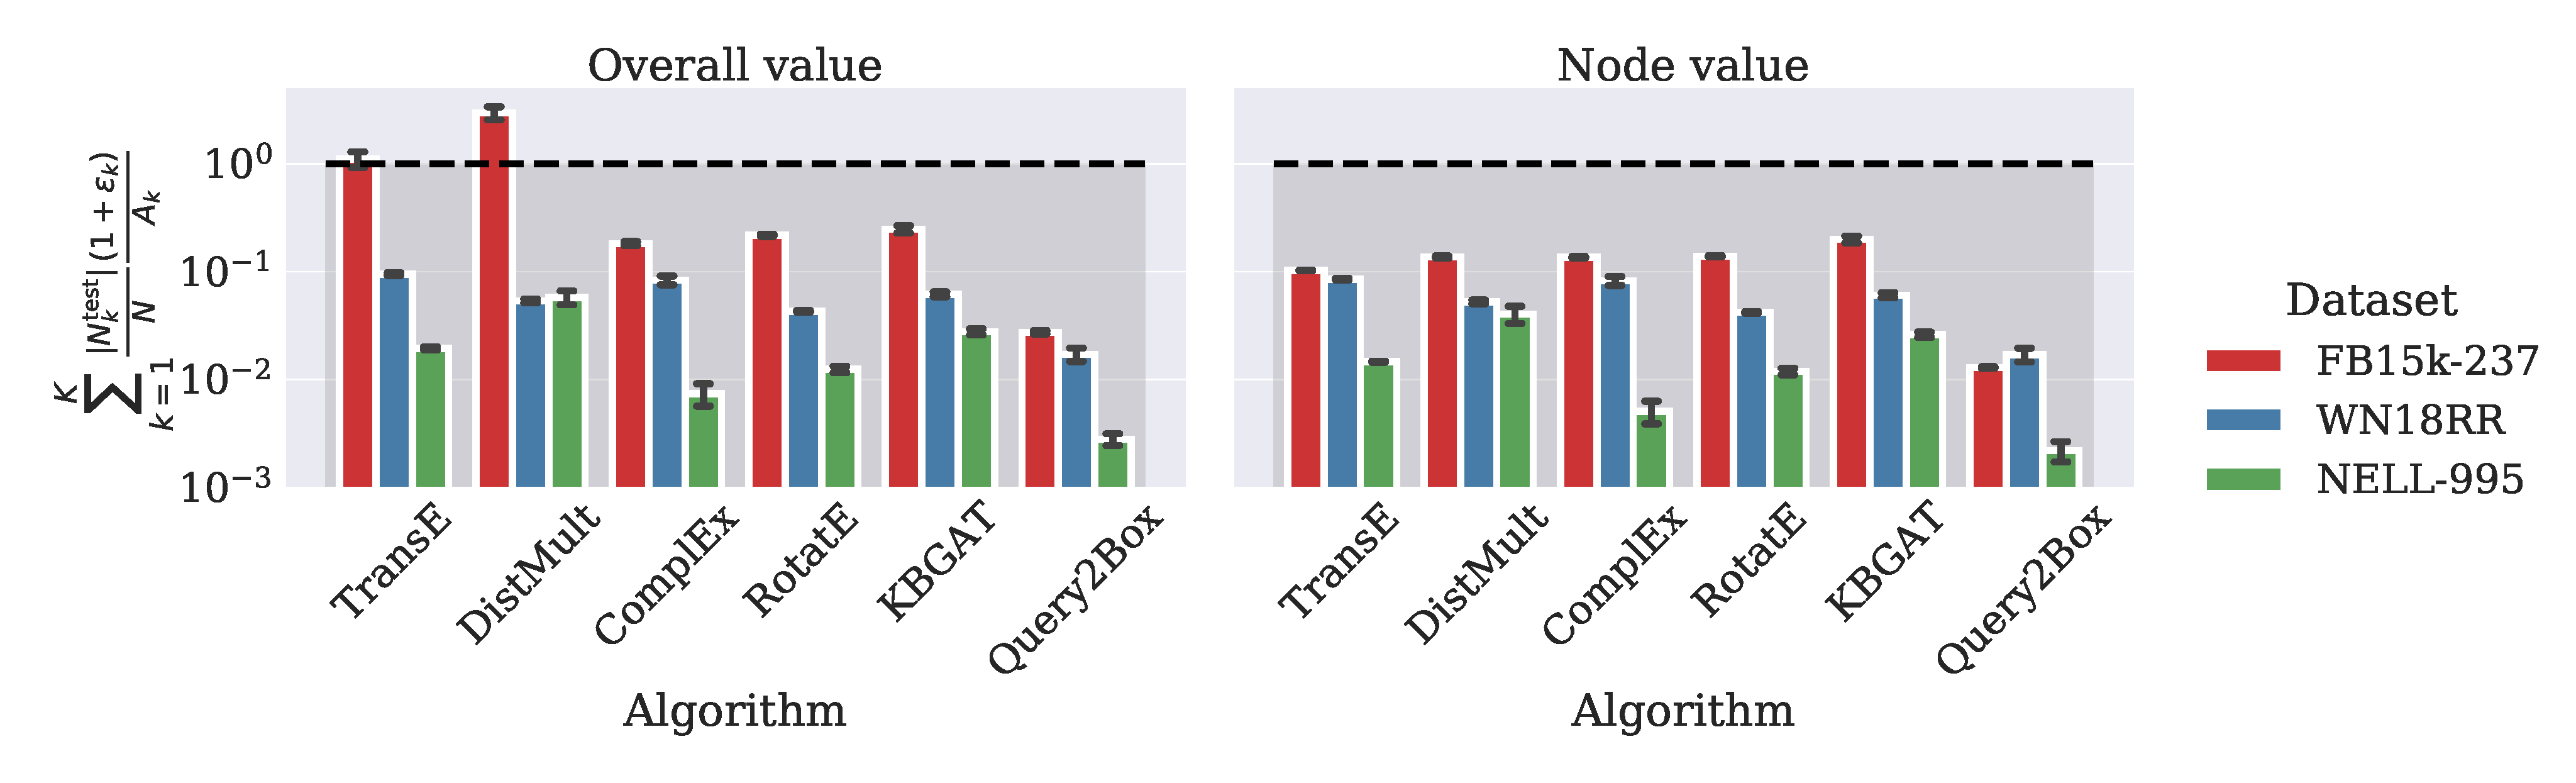
\includegraphics[width=\linewidth]{figures/coins/feasibility_statistic}
\end{center}
\caption[Plot of the values of the COINs feasibility statistic.]{Plot of values of the statistic from Proposition~\ref{proposition:condition_applicability} (lower is better). The feasible region is the one shaded. Left vs. right: statistic values computed from mean ranks after both steps vs. just the second step of COINs.}
\label{fig:feasibility_statistic}
\end{figure}

% \newpage

Figure~\ref{fig:feasibility_trajectories} aims to integrate community assignment validation with model feasibility analysis to explore the tradeoff between achieved community quality (measured by cut size, the count of inter-community edges affecting overparametrization), and the Proposition~\ref{proposition:condition_applicability} statistic (influenced by relative performance error and acceleration). 

To facilitate this tradeoff analysis, we conducted end-to-end training and evaluation for the COINs-RotatE combination on each dataset using various sources of community assignments. Specifically, we varied the Leiden resolution hyperparameter value, considered METIS for another case, and finally, communities assigned uniformly at random.

\begin{figure}[!ht]
\begin{center}
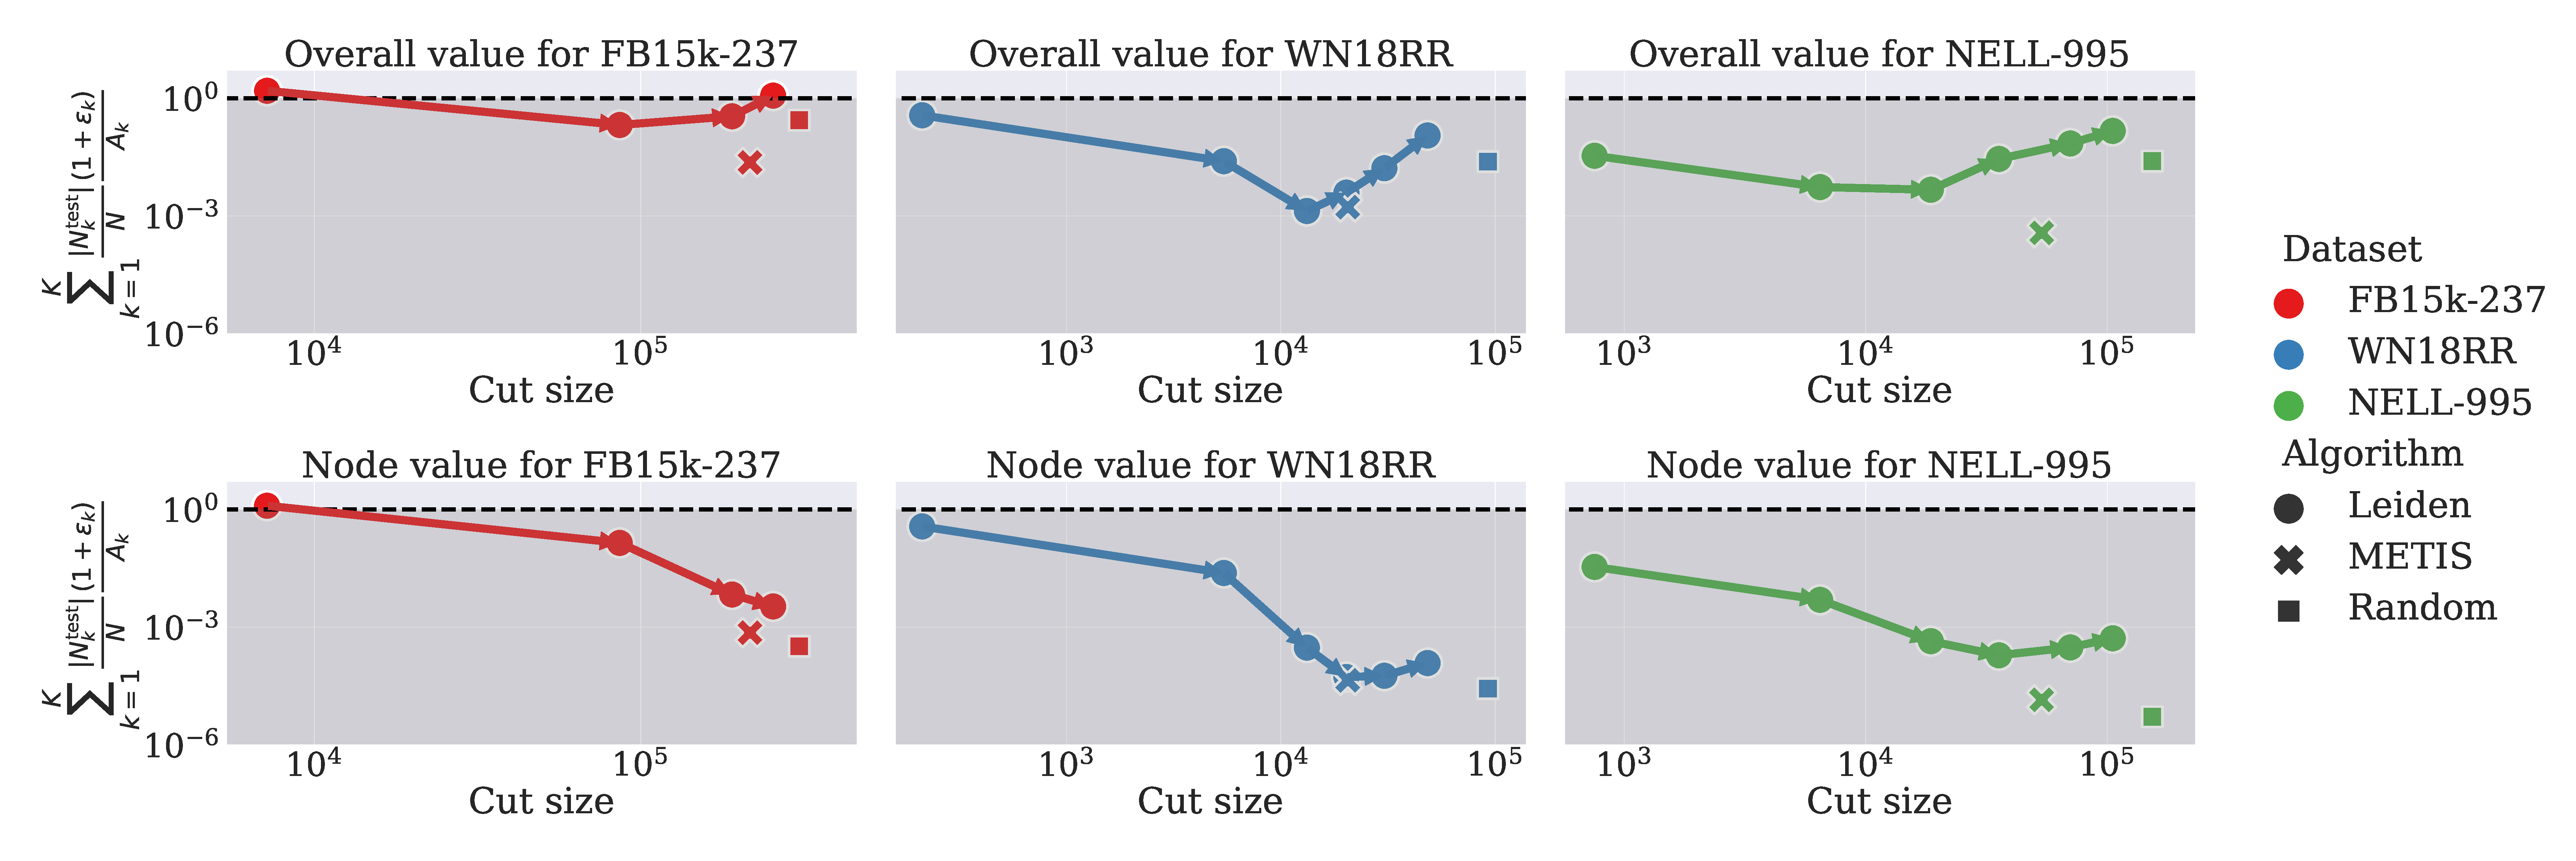
\includegraphics[width=\linewidth]{figures/coins/feasibility_extra}
\end{center}
\caption[Plot of trajectories in the performance-scalability space, for the RotatE algorithm trained and evaluated with different community assignments.]{Plot of trajectories in the performance-scalability space, for the RotatE algorithm trained and evaluated with different community assignments. It is better to have lower cut sizes and lower values of the statistic. The Leiden paths are obtained by varying the resolution hyperparameter, the direction of the arrows indicates an increase of resolution. The feasible region for the statistic from Proposition~\ref{proposition:condition_applicability} is the one shaded. Top vs. bottom: statistic values computed from mean ranks after both steps vs. just the second step of COINs. Left to right: different datasets.}
\label{fig:feasibility_trajectories}
\end{figure}

Leiden trajectories for all datasets possess a critical point in the statistic, revealing the existence of an optimal trade-off between relative error and acceleration. Cut sizes, however, exhibit a simple increase as Leiden resolution increases. For FB15k-237, we cross the feasibility boundary of Proposition~\ref{proposition:condition_applicability} by adjusting the resolution. 

When focusing solely on performance in the second prediction step, relative error improves more rapidly with Leiden resolution, resulting in lower values for the statistic. It is noteworthy that this is anticipated, as higher Leiden resolution implies smaller communities, leading to fewer possible query answers. 

Finally, we affirm that although METIS and random communities may yield higher speed-ups, numerous Leiden community assignments achieve comparable performance with equally significant speed-ups but considerably smaller cut sizes, thereby reducing the number of model parameters.

Table~\ref{tab:performance_link_prediction} contains all of our results on the link prediction task. We do not possess baselines for these results due to the limited scope of the related work, which focuses only on an evaluation of the query answering task. Thus, we cannot perform a similar comparison as before. Regardless, the relative ordering of the metric values across settings is consistent with the query answering performance discussed previously.

\begin{table}[ht!]
  \caption[All computed link prediction metrics.]{All computed link prediction metrics (higher is better), with community prediction metrics also given separately.}
  \label{tab:performance_link_prediction}
  \centering
    \begin{adjustbox}{width=\textwidth}%{totalheight=\textheight-2.6\baselineskip}
\begin{tabular}{lllllll}
\toprule
         &           &         &                 Accuracy &                       F1 &                  ROC-AUC &                       AP \\
Dataset & Algorithm & Value &                          &                          &                          &                          \\
\midrule
FB15k-237 & TransE & Community &    ${{0.946}_{\pm 0.0}}$ &    ${{0.941}_{\pm 0.0}}$ &    ${{0.964}_{\pm 0.0}}$ &  ${{0.812}_{\pm 0.005}}$ \\
         &           & Overall &  ${{0.895}_{\pm 0.001}}$ &  ${{0.896}_{\pm 0.001}}$ &     ${{0.94}_{\pm 0.0}}$ &  ${{0.727}_{\pm 0.003}}$ \\
         & DistMult & Community &  ${{0.864}_{\pm 0.007}}$ &  ${{0.877}_{\pm 0.006}}$ &   ${{0.97}_{\pm 0.004}}$ &  ${{0.861}_{\pm 0.016}}$ \\
         &           & Overall &  ${{0.908}_{\pm 0.002}}$ &  ${{0.912}_{\pm 0.001}}$ &   ${{0.95}_{\pm 0.001}}$ &  ${{0.841}_{\pm 0.005}}$ \\
         & ComplEx & Community &    ${{0.997}_{\pm 0.0}}$ &    ${{0.997}_{\pm 0.0}}$ &    ${{0.998}_{\pm 0.0}}$ &    ${{0.996}_{\pm 0.0}}$ \\
         &           & Overall &  ${{0.938}_{\pm 0.004}}$ &  ${{0.938}_{\pm 0.003}}$ &    ${{0.968}_{\pm 0.0}}$ &    ${{0.9}_{\pm 0.002}}$ \\
         & RotatE & Community &  ${{0.988}_{\pm 0.001}}$ &  ${{0.989}_{\pm 0.001}}$ &    ${{0.998}_{\pm 0.0}}$ &    ${{0.995}_{\pm 0.0}}$ \\
         &           & Overall &  ${{0.925}_{\pm 0.001}}$ &  ${{0.922}_{\pm 0.001}}$ &   ${{0.96}_{\pm 0.001}}$ &  ${{0.853}_{\pm 0.003}}$ \\
         & KBGAT & Community &    ${{0.995}_{\pm 0.0}}$ &    ${{0.995}_{\pm 0.0}}$ &    ${{0.999}_{\pm 0.0}}$ &    ${{0.998}_{\pm 0.0}}$ \\
         &           & Overall &  ${{0.884}_{\pm 0.005}}$ &  ${{0.858}_{\pm 0.008}}$ &  ${{0.935}_{\pm 0.007}}$ &  ${{0.789}_{\pm 0.019}}$ \\
         & Query2Box & Community &  ${{0.835}_{\pm 0.003}}$ &  ${{0.762}_{\pm 0.007}}$ &    ${{0.992}_{\pm 0.0}}$ &    ${{0.977}_{\pm 0.0}}$ \\
         &           & Overall &    ${{0.833}_{\pm 0.0}}$ &    ${{0.758}_{\pm 0.0}}$ &  ${{0.918}_{\pm 0.001}}$ &  ${{0.747}_{\pm 0.004}}$ \\
\midrule
WN18RR & TransE & Community &    ${{0.989}_{\pm 0.0}}$ &    ${{0.989}_{\pm 0.0}}$ &    ${{0.986}_{\pm 0.0}}$ &  ${{0.963}_{\pm 0.006}}$ \\
         &           & Overall &  ${{0.905}_{\pm 0.002}}$ &  ${{0.904}_{\pm 0.001}}$ &  ${{0.923}_{\pm 0.001}}$ &  ${{0.798}_{\pm 0.005}}$ \\
         & DistMult & Community &  ${{0.882}_{\pm 0.003}}$ &  ${{0.893}_{\pm 0.002}}$ &    ${{0.999}_{\pm 0.0}}$ &    ${{0.998}_{\pm 0.0}}$ \\
         &           & Overall &   ${{0.92}_{\pm 0.002}}$ &  ${{0.913}_{\pm 0.002}}$ &   ${{0.86}_{\pm 0.003}}$ &  ${{0.752}_{\pm 0.005}}$ \\
         & ComplEx & Community &      ${{1.0}_{\pm 0.0}}$ &      ${{1.0}_{\pm 0.0}}$ &      ${{1.0}_{\pm 0.0}}$ &      ${{1.0}_{\pm 0.0}}$ \\
         &           & Overall &  ${{0.925}_{\pm 0.001}}$ &  ${{0.917}_{\pm 0.001}}$ &  ${{0.912}_{\pm 0.001}}$ &  ${{0.814}_{\pm 0.001}}$ \\
         & RotatE & Community &    ${{0.997}_{\pm 0.0}}$ &    ${{0.997}_{\pm 0.0}}$ &    ${{0.999}_{\pm 0.0}}$ &    ${{0.999}_{\pm 0.0}}$ \\
         &           & Overall &    ${{0.912}_{\pm 0.0}}$ &      ${{0.9}_{\pm 0.0}}$ &  ${{0.949}_{\pm 0.001}}$ &  ${{0.871}_{\pm 0.001}}$ \\
         & KBGAT & Community &    ${{0.999}_{\pm 0.0}}$ &    ${{0.999}_{\pm 0.0}}$ &      ${{1.0}_{\pm 0.0}}$ &    ${{0.999}_{\pm 0.0}}$ \\
         &           & Overall &  ${{0.917}_{\pm 0.002}}$ &  ${{0.906}_{\pm 0.003}}$ &  ${{0.936}_{\pm 0.003}}$ &   ${{0.86}_{\pm 0.003}}$ \\
         & Query2Box & Community &  ${{0.837}_{\pm 0.003}}$ &  ${{0.766}_{\pm 0.007}}$ &    ${{0.999}_{\pm 0.0}}$ &    ${{0.999}_{\pm 0.0}}$ \\
         &           & Overall &    ${{0.833}_{\pm 0.0}}$ &    ${{0.758}_{\pm 0.0}}$ &  ${{0.888}_{\pm 0.003}}$ &   ${{0.68}_{\pm 0.008}}$ \\
\midrule
NELL-995 & TransE & Community &    ${{0.995}_{\pm 0.0}}$ &    ${{0.995}_{\pm 0.0}}$ &  ${{0.992}_{\pm 0.002}}$ &  ${{0.982}_{\pm 0.002}}$ \\
         &           & Overall &  ${{0.932}_{\pm 0.001}}$ &  ${{0.933}_{\pm 0.001}}$ &  ${{0.963}_{\pm 0.001}}$ &  ${{0.818}_{\pm 0.009}}$ \\
         & DistMult & Community &   ${{0.95}_{\pm 0.003}}$ &  ${{0.952}_{\pm 0.003}}$ &  ${{0.996}_{\pm 0.001}}$ &  ${{0.978}_{\pm 0.007}}$ \\
         &           & Overall &  ${{0.943}_{\pm 0.002}}$ &  ${{0.943}_{\pm 0.002}}$ &  ${{0.931}_{\pm 0.002}}$ &  ${{0.836}_{\pm 0.006}}$ \\
         & ComplEx & Community &    ${{0.999}_{\pm 0.0}}$ &    ${{0.999}_{\pm 0.0}}$ &    ${{0.999}_{\pm 0.0}}$ &    ${{0.999}_{\pm 0.0}}$ \\
         &           & Overall &  ${{0.968}_{\pm 0.001}}$ &  ${{0.968}_{\pm 0.001}}$ &     ${{0.99}_{\pm 0.0}}$ &  ${{0.961}_{\pm 0.002}}$ \\
         & RotatE & Community &  ${{0.993}_{\pm 0.001}}$ &  ${{0.993}_{\pm 0.001}}$ &      ${{1.0}_{\pm 0.0}}$ &    ${{0.999}_{\pm 0.0}}$ \\
         &           & Overall &  ${{0.947}_{\pm 0.004}}$ &  ${{0.945}_{\pm 0.004}}$ &  ${{0.977}_{\pm 0.001}}$ &  ${{0.885}_{\pm 0.009}}$ \\
         & KBGAT & Community &    ${{0.999}_{\pm 0.0}}$ &    ${{0.999}_{\pm 0.0}}$ &      ${{1.0}_{\pm 0.0}}$ &      ${{1.0}_{\pm 0.0}}$ \\
         &           & Overall &  ${{0.944}_{\pm 0.005}}$ &  ${{0.939}_{\pm 0.006}}$ &  ${{0.985}_{\pm 0.001}}$ &  ${{0.957}_{\pm 0.002}}$ \\
         & Query2Box & Community &  ${{0.834}_{\pm 0.001}}$ &  ${{0.759}_{\pm 0.002}}$ &    ${{0.999}_{\pm 0.0}}$ &  ${{0.998}_{\pm 0.001}}$ \\
         &           & Overall &    ${{0.833}_{\pm 0.0}}$ &    ${{0.758}_{\pm 0.0}}$ &  ${{0.963}_{\pm 0.002}}$ &  ${{0.882}_{\pm 0.005}}$ \\
\bottomrule
\end{tabular}
  \end{adjustbox}
\end{table}%

% Figure~\ref{fig:feasibility_trajectories} is our most detailed experiment, with the goal of merging together the validation of community assignments with the analysis of model feasibility, to investigate the tradeoff between achieved community quality, relative error in performance and acceleration/overparametrization. To facilitate this, for each dataset we end-to-end trained and evaluated the COINs-RotatE combination (as our most successful) with different sources of community assignments. Namely, we searched the region around the optimal value for the Leiden resolution hyperparameter to obtain worse communities, replaced Leiden with METIS for another case, and for a final run picked one random uniform community assignment.

% As in Figures~\ref{fig:scalability_resolution} and~\ref{fig:scalability_cut_size}, we observe that the Leiden trajectories for all datasets have a critical point with an optimal trade-off between relative error and acceleration. We note that overall relative error, although unstable w.r.t. Leiden resolution, does not vary greatly and the main differences seem to lie in the acceleration values (although for FB15k-237 we manage to enter and exit the feasibility region by changing resolution). On the other hand, when considering only the performance in the second prediction step, relative error improves with Leiden resolution much faster. Note that, however, this is to be expected, as greater Leiden resolution implies smaller communities and thus, fewer possible answers to queries. We confirm again that overparametrization simply increases with greater resolution values and dominates the trajectory direction in the overall performance case. Thus, we confirm again that although the METIS and random communities might yield higher speed-ups, there are a lot of Leiden community assignments resulting in similar performance, and equally significant speed-ups but with significantly fewer parameters. 

% \begin{figure}[ht!]
% \begin{center}
% \includegraphics[width=\textwidth]{figures/feasibility_rebuttals}
% \includegraphics[width=\textwidth]{figures/feasibility_rebuttals_2}
% \end{center}
% \caption{Plot of trajectories in the performance-scalability space, for the RotatE algorithm trained and evaluated with different community assignments. The Leiden paths are obtained by varying the resolution hyperparameter, the direction of the arrows indicates an increase of resolution. The feasible region for acceleration (Proposition~\ref{proposition:condition_applicability}) is the one shaded. Odd vs. even rows: COINs metric values after both steps vs. just the second step. Top two vs. bottom two rows: acceleration vs. overparametrization space.}
% \label{fig:feasibility_trajectories}
% \end{figure}



\subsection{Stability \& Convergence}

The convergence plots in Figure~\ref{fig:convergence} support our decision to model the final aggregate COINs loss value as the linear combination of the community and node terms. From the convergence lines, one can observe that the community and node iterates seem to converge at equal rates in both training and validation data. As such, the aggregate COINs loss function can be a simple average of the two terms without affecting convergence.

\begin{figure}[!ht]
\begin{center}
\includegraphics[width=\textwidth]{figures/coins/convergence}
\end{center}
\caption[Plots of contrastive loss convergence over time.]{Plots of contrastive loss convergence over time, with the decomposition of the final COINs loss into the two constituent community and node loss terms. Top vs. bottom: training vs. validation loss. Left to right: the different COINs-integrated algorithms. Error bands show standard deviation across datasets.}
\label{fig:convergence}
\end{figure}

% \clearpage

\section{Practical speed-ups}
All of the discussion on the acceleration benefits of COINs so far only concerned the reduction in computational complexity, i.e. how much fewer embedding operations are performed during evaluation. For completeness, we also estimated the speed-up one would observe in practice, i.e. the reduction in total CPU seconds of the evaluation process compared to the baseline. 

From the visualization of these results in Figure~\ref{fig:acceleration_wall} we can deduce that even w.r.t. wall time COINs always provides at least around 2 times speed-up, while the time-memory trade-off employed by NodePiece and EARL is also evident. The slow-down factors incurred by these methods are too great to justify the comparatively smaller memory-usage reduction factors. However, due to high variance in the experiment conditions during measurement, as well as differences in the practical complexity of the embedding algorithm implementations, these acceleration numerics are inconsistent across different settings and with large error bars. For such reasons, we relied mainly on the more reliable measurements of computation steps.

\begin{figure}[ht!]
\begin{center}
\includegraphics[width=\textwidth]{figures/coins/acceleration_wall}
\end{center}
\caption[CPU time speed-up thanks to COINs.]{Per-algorithm evaluation CPU time speed-up thanks to COINs, averaged across multiple seeds. Left to right: different datasets.}
\label{fig:acceleration_wall}
\end{figure}

\section{Implementation details}
\label{sec:appendix_implementation}

The entire implementation was performed in the Python 3.6 programming language. The Pandas library~\cite{mckinney_data_2010} was helpful with its efficient preprocessing operations on tabular data. The iGraph library~\cite{csardi_igraph_2005} was utilized for the implementation of most of the graph analysis and preprocessing steps, including executing the Leiden algorithm. For METIS, the official software implementation~\cite{karypis_metis_1997} was invoked through a Python wrapper. 

The entire model architecture (along with integration code for the publicly available implementations of the external embedders), training, and evaluation, were implemented using the PyTorch deep learning framework~\cite{paszke_pytorch_2019} and the extension framework for graph neural network learning PyTorch Geometric~\cite{fey_fast_2019}. 

All code was executed on a single machine with the following specifications:
\begin{itemize}
    % \item Intel\textsuperscript{\textregistered} Xeon\textsuperscript{\textregistered} Gold 5118 12-core CPU @ 2.30GHz;
    % \item NVIDIA Tesla P100-PCIE-16GB GPU;
    % \item 64GB RAM.
    \item AMD EPYC\textsuperscript{\texttrademark} 7742 64-core CPU @ 2.25GHz;
    \item NVIDIA A100-SXM4-40GB GPU;
    \item 1.0TB RAM. 
\end{itemize}

% To facilitate reproducibility, our full code implementation is available at: \\
% \url{https://github.com/LIONS-EPFL/coins-ict-innovations-2025}.

% \section{Appendix}
% Any possible appendices should be placed after bibliographies.
% If your paper has appendices, please submit the appendices together with the main body of the paper.
% There will be no separate supplementary material submission.
% The main text should be self-contained; reviewers are not obliged to look at the appendices when writing their review comments.


% \section{First Section}
% \subsection{A Subsection Sample}
% Please note that the first paragraph of a section or subsection is
% not indented. The first paragraph that follows a table, figure,
% equation etc. does not need an indent, either.

% Subsequent paragraphs, however, are indented.

% \subsubsection{Sample Heading (Third Level)} Only two levels of
% headings should be numbered. Lower level headings remain unnumbered;
% they are formatted as run-in headings.

% \paragraph{Sample Heading (Fourth Level)}
% The contribution should contain no more than four levels of
% headings. Table~\ref{tab1} gives a summary of all heading levels.

% \begin{table}
% \caption{Table captions should be placed above the
% tables.}\label{tab1}
% \begin{tabular}{lll}
% \hline
% Heading level &  Example & Font size and style\\
% \hline
% Title (centered) &  {\Large\bfseries Lecture Notes} & 14 point, bold\\
% 1st-level heading &  {\large\bfseries 1 Introduction} & 12 point, bold\\
% 2nd-level heading & {\bfseries 2.1 Printing Area} & 10 point, bold\\
% 3rd-level heading & {\bfseries Run-in Heading in Bold.} Text follows & 10 point, bold\\
% 4th-level heading & {\itshape Lowest Level Heading.} Text follows & 10 point, italic\\
% \hline
% \end{tabular}
% \end{table}


% \noindent Displayed equations are centered and set on a separate
% line.
% \begin{equation}
% x + y = z
% \end{equation}
% Please try to avoid rasterized images for line-art diagrams and
% schemas. Whenever possible, use vector graphics instead (see
% Fig.~\ref{fig1}).

% \begin{figure}
% \includegraphics[width=\textwidth]{fig1.eps}
% \caption{A figure caption is always placed below the illustration.
% Please note that short captions are centered, while long ones are
% justified by the macro package automatically.} \label{fig1}
% \end{figure}

% \begin{theorem}
% This is a sample theorem. The run-in heading is set in bold, while
% the following text appears in italics. Definitions, lemmas,
% propositions, and corollaries are styled the same way.
% \end{theorem}
% %
% % the environments 'definition', 'lemma', 'proposition', 'corollary',
% % 'remark', and 'example' are defined in the LLNCS documentclass as well.
% %
% \begin{proof}
% Proofs, examples, and remarks have the initial word in italics,
% while the following text appears in normal font.
% \end{proof}
% For citations of references, we prefer the use of square brackets
% and consecutive numbers. Citations using labels or the author/year
% convention are also acceptable. The following bibliography provides
% a sample reference list with entries for journal
% articles~\cite{ref_article1}, an LNCS chapter~\cite{ref_lncs1}, a
% book~\cite{ref_book1}, proceedings without editors~\cite{ref_proc1},
% and a homepage~\cite{ref_url1}. Multiple citations are grouped
% \cite{ref_article1,ref_lncs1,ref_book1},
% \cite{ref_article1,ref_book1,ref_proc1,ref_url1}.

\chapter{Appendix for HiGenDiff}

\section{Proofs}
\label{sec:appendix_higendiff_theory}

\begin{proof}[Proposition~\ref{proposition:complexity_higendiff}]
Let $\offf{c^{\of{L}}_k}_{k=1}^{n^{\of{L+1}}}$ be the sizes of the communities imposed by $M^{\of{L}}$, i.e., $\forall k, c^{\of{L}}_k=\sum_{i=1}^{n^{\of{L}}}{M^{\of{L}}_{k,i}}$. Then the worst-case cost of one diffusion step of HiGenDiff for a given adjacency matrix $A^{\of{L}}$ will be thus ${n^{\of{L+1}}}^2 + \sum_{j=1}^{n^{\of{L+1}}}\sum_{k=1}^{n^{\of{L+1}}}{c^{\of{L}}_j c^{\of{L}}_k \bar{A}_{j,k}^{\of{L+1}}}$. This is because we need to sample all the edges of the parent graph and then sample all communities and the bipartites that should exist, according to the parent level's adjacency. Since all the above quantities are random variables, under the i.i.d. Bernoulli assumption the expectation yields:
\begin{align}
    \begin{split}
        \mathbb{E}\off{{n^{\of{L+1}}}^2 + \sum_{j=1}^{n^{\of{L+1}}}\sum_{k=1}^{n^{\of{L+1}}}{c^{\of{L}}_j c^{\of{L}}_k \bar{A}_{j,k}^{\of{L+1}}}} 
        &= \mathbb{E}\off{{n^{\of{L+1}}}^2}+\sum_{j=1}^{n^{\of{L+1}}}\sum_{k=1}^{n^{\of{L+1}}}{\mathbb{E}\off{c^{\of{L}}_j c^{\of{L}}_k} \mathbb{E}\off{\bar{A}_{j,k}^{\of{L+1}}}} \\
        &= \mathbb{E}\off{{n^{\of{L+1}}}^2}+p\sum_{j=1}^{n^{\of{L+1}}}\sum_{k=1}^{n^{\of{L+1}}}{\of{\mathrm{Cov}\off{c^{\of{L}}_j,c^{\of{L}}_k}+\mathbb{E}\off{c^{\of{L}}_j}\mathbb{E}\off{c^{\of{L}}_k}}} \\
        &= \mathbb{E}\off{{n^{\of{L+1}}}^2}+p\of{\mathrm{Cov}\off{\sum_{j=1}^{n^{\of{L+1}}}{c^{\of{L}}_j},\sum_{k=1}^{n^{\of{L+1}}}{c^{\of{L}}_k}}+\mathbb{E}\off{\sum_{k=1}^{n^{\of{L+1}}}{c^{\of{L}}_k}}^2}\\
         &= \mathbb{E}\off{{n^{\of{L+1}}}^2} +p \of{\mathbb{V}\off{n^{\of{L}}}+\mathbb{E}\off{n^{\of{L}}}^2} \\
          &= \mathbb{E}\off{{n^{\of{L+1}}}^2} + p\mathbb{E}\off{{n^{\of{L}}}^2}
    \end{split}
\end{align}
For the upper bound, note that always $p \leq 1$ and $n^{\of{L+1}} \leq n^{\of{L}}$.

For the lower bound, we know that $p \geq \frac{1}{n^{\of{L+1}}}$, as in the best case, there will not be a single bipartite to generate, but we always have to sample the communities (the self-loops in the parent). Thus taking the expectation of $p$ w.r.t. $n^{\of{L}}$ implies: $\mathbb{E}\off{{n^{\of{L+1}}}^2} +p\mathbb{E}\off{{n^{\of{L}}}^2} \geq \mathbb{E}\off{{n^{\of{L+1}}}^2 + \frac{{n^{\of{L}}}^2}{n^{\of{L+1}}}}$. Similar to the proof of Proposition \ref{proposition:complexity_distributed}, we find that the minimum of the function $f\of{K}=K^2+\frac{\abs{V}}{K}$ is $\frac{3}{2}\sqrt[3]{2\abs{V}^2}$ and is achieved when $K=\frac{1}{2}\sqrt[3]{4\abs{V}}$. Plugging in $\abs{V}={n^{\of{L}}}^2$ and $K=n^{\of{L+1}}$ yields the result.
\end{proof}

\section{Detailed results}
\label{sec:appendix_higendiff_results}

\begin{table}[H]
    \centering
\caption[All MMD metrics for HiGenDiff.]{All MMD metrics (lower is better) for HiGenDiff of the model ablation experiments for each dataset.}
\label{tab:higendiff_full}
\begin{adjustbox}{width=\textwidth}
    \begin{tabular}{lllrrrr}
\toprule
 &  &  & Degree MMD & Cluster MMD & Orbit MMD & Spectral MMD \\
Dataset & Model & Bucketized &  &  &  &  \\
\midrule
\multirow[t]{5}{*}{enzyme} & Simple & No & 0.002 & 0.018 & 0.046 & 0.008 \\
% \cline{2-7}
 & \multirow[t]{2}{*}{Integer} & No & 0.007 & 0.019 & 0.048 & 0.01 \\
 &  & Yes & 0.004 & 0.016 & 0.025 & 0.005 \\
% \cline{2-7}
 & \multirow[t]{2}{*}{Ordinal} & No & 0.007 & 0.018 & 0.034 & 0.007 \\
 &  & Yes & 0.004 & 0.019 & 0.043 & 0.008 \\
% \cline{1-7} \cline{2-7}
\midrule
\multirow[t]{5}{*}{SBM} & Simple & No & 0.002 & 0.03 & 0.044 & 0.004 \\
% \cline{2-7}
 & \multirow[t]{2}{*}{Integer} & No & 0.001 & 0.028 & 0.047 & 0.004 \\
 &  & Yes & 0.001 & 0.027 & 0.04 & 0.004 \\
% \cline{2-7}
 & \multirow[t]{2}{*}{Ordinal} & No & 0.001 & 0.029 & 0.046 & 0.004 \\
 &  & Yes & 0.001 & 0.03 & 0.068 & 0.005 \\
% \cline{1-7} \cline{2-7}
\midrule
\multirow[t]{5}{*}{Ego2} & Simple & No & 0.002 & 0.06 & 0.036 & 0.005 \\
% \cline{2-7}
 & \multirow[t]{2}{*}{Integer} & No & 0.002 & 0.065 & 0.033 & 0.003 \\
 &  & Yes & 0.002 & 0.055 & 0.053 & 0.007 \\
% \cline{2-7}
 & \multirow[t]{2}{*}{Ordinal} & No & 0.011 & 0.064 & 0.035 & 0.02 \\
 &  & Yes & 0.002 & 0.059 & 0.042 & 0.004 \\
% \cline{1-7} \cline{2-7}
\midrule
\multirow[t]{5}{*}{DD2} & Simple & No & 0.004 & 0.08 & 0.024 & 0.005 \\
% \cline{2-7}
 & \multirow[t]{2}{*}{Integer} & No & 0.009 & 0.092 & 0.05 & 0.007 \\
 &  & Yes & 0.013 & 0.109 & 0.035 & 0.008 \\
% \cline{2-7}
 & \multirow[t]{2}{*}{Ordinal} & No & 0.002 & 0.072 & 0.112 & 0.007 \\
 &  & Yes & 0.008 & 0.09 & 0.031 & 0.007 \\
% \cline{1-7} \cline{2-7}
\midrule
\multirow[t]{5}{*}{RoC} & Simple & No & 0.003 & 0.218 & 0.002 & 0.027 \\
% \cline{2-7}
 & \multirow[t]{2}{*}{Integer} & No & 0.013 & 0.312 & 0.014 & 0.044 \\
 &  & Yes & 0.008 & 0.266 & 0.018 & 0.039 \\
% \cline{2-7}
 & \multirow[t]{2}{*}{Ordinal} & No & 0.015 & 0.297 & 0.029 & 0.044 \\
 &  & Yes & 0.01 & 0.298 & 0.019 & 0.041 \\
% \cline{1-7} \cline{2-7}
\midrule
\multirow[t]{5}{*}{LFR} & Simple & No & 0.022 & 0.214 & 0.12 & 0.004 \\
% \cline{2-7}
 & \multirow[t]{2}{*}{Integer} & No & 0.103 & 0.309 & 0.448 & 0.055 \\
 &  & Yes & 0.037 & 0.05 & 0.162 & 0.012 \\
% \cline{2-7}
 & \multirow[t]{2}{*}{Ordinal} & No & 0.086 & 0.202 & 0.364 & 0.042 \\
 &  & Yes & 0.023 & 0.33 & 0.184 & 0.009 \\
% \cline{1-7} \cline{2-7}
\bottomrule
\end{tabular}
\end{adjustbox}
\end{table}

\chapter{Appendix for MultiProx}

\section{A principled multi-measurement sampling framework}
\label{sec:appendix_gibbs}
\subsection{Multi-measurement model}
Let $\mathbf{X}_0 \sim p_0$. Let $t>0$ be a fixed noise level. We define $m$, correlated, noisy measurements $\of{\mathbf{Y}_1, \dots, \mathbf{Y}_m}$ of $X$, at noise level $t >0$, as
\begin{equation}
\mathbf{Y}_i = e^{-t} \mathbf{X} + \sqrt{1 - e^{-2t}} Z_i
\label{eq:multimeasure}
\end{equation}
where $Z_1, \dots, Z_m$ are independent $N\of{\mathbf{0}, \mathbf{I}_F}$ variables. These $m$ measurements are correlated through $\mathbf{X}$. Our method builds on the observation from \cite{saremi_multimeasurement_2021} that denoising from an entire set of correlated noisy measurements $\of{\mathbf{Y}_1, \dots, \mathbf{Y}_m}$ is easier than denoising from a single noisy measurement. The multimeasurement sampling framework we analyze in this section consists of generating $\mathbf{X}_0$ by denoising from the $m$ fixed-noise level measurements $\of{\mathbf{Y}_1, \dots, \mathbf{Y}_m}$. Unlike DDPMs, this framework does not progressively denoise following an annealing schedule. It consists of two components: a denoising component that produces a sample $\mathbf{X}_0$ from the noisy measurements and an initialization component that generates the noisy measurements $\of{\mathbf{Y}_1, \dots, \mathbf{Y}_m}$ to denoise from. We summarize the framework in Algorithm \ref{alg:pipeline} and explain its soundness in detail in what follows.

\begin{algorithm}[H]
\caption{Gibbs Multi-measurement Sampling Framework}
\label{alg:pipeline}
\begin{algorithmic}
\STATE{\textbf{input} $m,t\geq0$}
\STATE{$\of{\mathbf{Y}_1, \dots, \mathbf{Y}_m} \sim N\of{\mathbf{0}, \mathbf{I}_{m F}}$}
\FOR{$i \gets 1 \text{ to } m$}
\STATE{$\mathbf{Y}_i \sim \mathbf{Y}_i|\mathbf{Y}_{-i}$}
\ENDFOR
\RETURN{$\mathbf{X} \sim \mathbf{X}|\mathbf{Y}_{1,\dots,m}$}
\end{algorithmic}
\end{algorithm}

\subsection{Denoising from multiple measurements}
We first consider the denoising component: the process generating $\mathbf{X}_0$ from $\of{\mathbf{Y}_1, \dots, \mathbf{Y}_m}$. This can be achieved by sampling from the conditional distribution $\mathbf{X}_0|\of{\mathbf{Y}_1, \dots, \mathbf{Y}_m}$. Fortunately, for any noise level $t$, the denoising distribution $\mathbf{X}_0|\of{\mathbf{Y}_1, \dots, \mathbf{Y}_m}$ can be made to be unimodal by accumulating enough measurements, i.e., by choosing $m$ large enough. This follows from the simple observation that the average of the $m$ measurements yields
\begin{equation}
\frac{1}{m}\sum_{i=1}^m \mathbf{Y}_i \overset{\mathcal{L}}{=}  e^{-t} \mathbf{X} + \sqrt{\frac{1 - e^{-2t}}{m}}Z
\label{eq:noisereduction}
\end{equation}
where $Z \sim N\of{\mathbf{0}, \mathbf{I}_F}$, which reduces the amount of noise by a factor $\sqrt{m}$. The parameter $m$ can thus be set to compensate for a large choice of $t$. Indeed, as discussed in section \ref{sec:background_multiprox}, a large choice of $t$ is necessary in order to be able to initialize $\of{\mathbf{Y}_1, \dots, \mathbf{Y}_m}$ before denoising, but the denoising becomes increasingly difficult as multi-modality increases with $t$. With the parameter $m$, we can act on this trade-off to ensure that the denoising stays a unimodal sampling problem. We formally show this in the following theorem. 

\begin{theorem}
\label{thm:unimodality}
    Under the assumption that the score $\nabla \log p_0$ is $L$-Lipschitz, for any $t$ and $\mathbf{Y}_1, \dots, \mathbf{Y}_m$ defined as in \eqref{eq:multimeasure}, the Hessian of the conditional distribution $\mathbf{X}|\mathbf{Y}_1, \dots, \mathbf{Y}_m$ satisfies
    \begin{equation}
    \nabla ^2 \log p(x|y_1, \dots, y_m) \preceq \off{L - m\frac{e^{-2t}}{1 - e^{-2t}}}\mathbf{I}_F.
    \label{eq:concave}
    \end{equation}
\end{theorem}

According to \eqref{eq:concave}, as long as $m > \of{e^{2t} - 1} L$, the denoising distribution $\mathbf{X}_0|\of{\mathbf{Y}_1, \dots, \mathbf{Y}_m}$ is strongly-log-concave, i.e, unimodal, making the denoising tractable. Consequently, as long as a sample from $\of{\mathbf{Y}_1, \dots, \mathbf{Y}_m}$ can be obtained, a sample of $\mathbf{X}_0$ can obtained through sampling from a strongly log-concave distribution.

% \begin{remark}
%     Our result holds for log-smooth distributions (Assumption \ref{ass:log-smooth}), this assumption is standard in the analysis of denoising diffusions \cite{chen2022sampling, benton2023linear}. A alternative way of obtaining a log-smooth distribution is through Gaussian convolution of a bounded distribution: if $X$ is bounded, then $X + \sqrt{\delta}Z$, with $Z\sim \sN\br{0, I}$ is log-smooth. This convolution trick to obtain log-smooth distributions corresponds to the \emph{early-stopping} criterion assumption in convergence proofs of diffusion samplers.
% \end{remark}

\subsection{Sampling the noisy measurements}
We turn our attention to the initialization problem of obtaining a sample from  $\of{\mathbf{Y}_1, \dots, \mathbf{Y}_m}$. If $t$ is large, each $\mathbf{Y}_i$ approaches a standard Gaussian according to \eqref{eq:multimeasure}. The individual coordinates approximate standard Gaussians, but they must be appropriately correlated in order to accurately approximate $\of{\mathbf{Y}_1, \dots, \mathbf{Y}_m}$. Indeed, the benefit of multiple measurements follows from the correlation of the measurements and is a crucial component as the noise reduction in \eqref{eq:noisereduction} depends on it. 

Instead of sampling each coordinate by sequentially increasing the conditioning as in \cite{saremi_chain_2023}, we propose a Gibbs sampling strategy \cite{casella_explaining_1992, roberts_updating_1997}. Gibbs sampling consists of iteratively sampling each component $\mathbf{Y}_i$ conditioned on all the other $m-1$ measurements, denoted $\mathbf{Y}_{-i}$. Gibbs sampling is guaranteed to converge to the joint distribution \cite{rosenthal_minorization_1995} and is a well-studied strategy for sampling when each conditioned marginal is easy to sample from \cite{koller_probabilistic_2009}. The following theorem will help show that there exists a choice of $t$ such that each conditional marginal $\mathbf{Y}_i|\mathbf{Y}_{-i}$ is easy to sample from. 

\begin{theorem}
\label{thm:unimodality_conditional}
    Under the log-smoothness assumption again, for any, $t>0$ and $\mathbf{Y}_1, \dots, \mathbf{Y}_m$ as in \eqref{eq:multimeasure}, we have that for any  $i \in \off{m}$, the hessian of $\log p\of{y_i|y_{-i}}$ is given by
    \begin{align}
    \begin{split}
    \nabla^2_{y_i} \log p\of{y_i|y_{-i}} &= \mathbb{V}_{\mathbf{X}|\mathbf{Y}_1, \dots, \mathbf{Y}_m = (y_1, \dots, y_m)}\off{\frac{e^{-t} \mathbf{X} - y_i}{1 - e^{-2t}}} - \frac{1}{1-e^{-2t}}\mathbf{I}_F \\
    &= \of{\frac{e^{-t}}{1 - e^{-2t}}}^2\mathbb{V}_{\mathbf{X}|\mathbf{Y}_1, \dots, \mathbf{Y}_m =(y_1, \dots, y_m)}\off{\mathbf{X}} - \frac{1}{1-e^{-2t}}\mathbf{I}_F.
    \end{split}
    \end{align}
    \label{eq:conditionalunimodal}
\end{theorem}
In order to use the theorem above to show that the distributions are log-concave, we need to control the variance term in \eqref{eq:conditionalunimodal}. We can upper-bound this variance term using Bakry-Emery's result showing that strongly log-concave measures verify the Poincaré inequality.

\begin{theorem}
\label{thm:variance}
    Let $\mathbf{X}$ be an $L$-smooth density, if $m$ is such that $m \geq 2\of{e^{2t} - 1}L$, then it holds that
    \begin{equation}
       \mathbb{V}_{\mathbf{X}|\mathbf{Y}_1, \dots, \mathbf{Y}_m =(y_1, \dots, y_m)}\off{\mathbf{X}} \leq \frac{L}{2}.
    \end{equation}
\end{theorem}

Equipped with the result above, we can show that, in order for \eqref{eq:conditionalunimodal} to be negative, the noise level should be set such that
\begin{equation}
t \geq \frac{1}{2}\log\of{1 + \frac{L}{2}}.
\end{equation}

With the above conditions, we can show that our sampling framework, detailed in Algorithm \ref{alg:pipeline}, is a fully unimodal sampling pipeline. This was achieved not with annealing but with multiple measurements. Indeed, combining the previous theorems, we have that the following theorem holds for the Gibbs multi-measurement sampler.

\begin{theorem}
    \label{thm:logconcavepipe}
    Under the log-smoothness assumption, for $t> \frac{1}{2}\log\of{1 + \frac{L}{2}}$ and $m \geq 2\of{e^{2t} - 1}L$, we have that the framework of Algorithm \ref{alg:pipeline} is a fully log-concave pipeline, where each step only samples from a unimodal distribution.
\end{theorem}

\section{Additional experiments}
\label{sec:appendix_multiprox_experiments}

\begin{figure}[H]
    \centering
    \includegraphics[width=\linewidth]{figures/multiprox/comm20_grid_image_single_noise.png}
    \includegraphics[width=\linewidth]{figures/multiprox/comm20_grid_image.png}
    \caption[Best sample chains obtained with MultiProx and MultiProxAn employing a ConGress denoiser trained on Community20.]{Best sample chains obtained with MultiProx and MultiProxAn employing a ConGress denoiser trained on Community20. We set for these chains $n=10$, $m=100$, $t=75$ (15\% of $T$) for MultiProx and $t=200, t'=50$ (40\% and 10\% of $T$) for MultiProxAn.}
    \label{fig:comm20_extra}
\end{figure}

\begin{table}[H]
    \centering
    \caption[Sampling metrics for each MultiProxAn noise level hyperparameter configuration tested for the Community20 dataset.]{Sampling metrics for each noise level hyperparameter configuration we tested for the Community20 dataset. Left to right: MultiProxAn fixed noise level $t$ and final output noise level $t' \leq t$ (as percentages of $T$), Maximum Mean Discrepancy (MMD) metrics for node degrees, per-node clustering coefficients, node orbits, and node eigenvalues between sampled and dataset graph distributions, and total execution time of sampling. Arrows indicate whether higher or lower values of a metric are better. Best values per metric are in bold, while second-best values are underlined.}
    \label{tab:comm20_stats}
    \resizebox{\columnwidth}{!}{
    \begin{tabular}{llrrrrr}
        \toprule
         $t$ & $t'$ & $\downarrow$ Degree MMD & $\downarrow$ Cluster MMD & $\downarrow$ Orbit MMD & $\downarrow$ Spectral MMD & $\downarrow$ Wall time [s]  \\
         \midrule
         \multicolumn{2}{l}{Baseline} & 0.0064 & \textbf{0.0725} & \underline{0.0214} & \textbf{0.0232} & 846 \\
         40\% & 40\% & 0.1630 & 0.1230 & 0.6954 & 0.0718 & \textbf{139} \\
         40\% & 20\% & \textbf{0.0022} & 0.1148 & 0.0666 & 0.0633 & 305 \\
         40\% & 10\% & 0.0037 & 0.0864 & \textbf{0.0051} & 0.1219 & 388 \\
         40\% & 0.2\% & 0.0150 & \underline{0.0833} & 0.0376 & 0.1965 & 467 \\
         20\% & 20\% & 0.0527 & 0.1230 & 0.6039 & 0.0456 & \textbf{139} \\
         20\% & 10\% & 0.0067 & 0.1188 & 0.3760 & 0.0422 & 223 \\
         20\% & 0.2\% & \underline{0.0023} & 0.1152 & 0.2743 & \underline{0.0394} & 306 \\
         10\% & 10\% & 0.0734 & 0.1272 & 0.6653 & 0.0752 & \textbf{138} \\
         10\% & 0.2\% & 0.0699 & 0.1266 & 0.7000 & 0.0458 & \underline{222} \\
         \bottomrule
    \end{tabular}}
\end{table}

\section{Implementation}

For the molecule generation experiments, we extend the implementation of \cite{vignac_digress_2022} (available at \url{https://github.com/cvignac/DiGress}) with code for our novel specific sampling method tailored to the architecture of DiGress. Our experiment code implementation is fully available at \url{https://github.com/ResearchWeasel/multi-prox-diffusion-nips-2025} to facilitate reproducibility.

All code was executed on a single machine with the following specifications:
\begin{itemize}
    \item AMD EPYC\textsuperscript{\texttrademark} 7742 64-core CPU @ 2.25GHz;
    \item NVIDIA A100-SXM4-40GB GPU;
    \item 1.0TB RAM. 
\end{itemize}
\backmatter
\addcontentsline{toc}{chapter}{Bibliography}
\cleardoublepage
\phantomsection
% ************* The working stuff *************
% Print the bibliography just here

\printbibliography


% Add your glossary here
% Add your index here
% Photographic credits (list of pictures&images that have been used with names of the person holding the copyright for them)
\cleardoublepage
\thispagestyle{empty}
\phantomsection
\addcontentsline{toc}{chapter}{Curriculum Vitae}

% NOTE: If you want to make your life hard and write your CV in Latex keep the following lines as they are. If you desire to upload a pre-made PDF CV please uncomment the next line and comment the line just after it.
\includepdf[pagecommand=\thispagestyle{addpagenumbersforpdfimports},pages=-,noautoscale = true,width=\linewidth]{tail/cv/cv.pdf} % To upload a PDF CV directly
% \subfile{tail/cv/cv_main.tex} % To do cv with LaTeX

\end{document}
